%\documentclass[3p,times,procedia,number]{elsarticle}
\documentclass[3p,times,number,review]{elsarticle}
\usepackage{lineno}
\modulolinenumbers[5]

\flushbottom

%% The `ecrc' package must be called to make the CRC functionality available
\usepackage{ecrc}
\usepackage{amsmath}
\usepackage{cases}
\usepackage{amssymb}
\usepackage{mathtools}
\usepackage{bm}
\usepackage{verbatim}
%\usepackage[fleqn]{amsmath}
\usepackage{caption}
\usepackage{ulem}
\usepackage[colorlinks,linkcolor=blue,citecolor=blue,urlcolor=blue]{hyperref}
\usepackage{graphicx} 
\usepackage[subfigure]{graphfig}
\setcounter{totalnumber}{4}
\renewcommand{\textfraction}{0.15}
\renewcommand{\topfraction}{0.85}
\renewcommand{\bottomfraction}{0.65}
\renewcommand{\floatpagefraction}{0.60}
\newcommand{\figref}[1]{\figurename~\ref{#1}}
\usepackage{titlesec}
\titleformat{\chapter}[display]
{\normalfont\Large\bfseries}{\thechapter}{11pt}{\Large}
\titleformat{\section}
{\normalfont\large\bfseries}{\thesection}{11pt}{\large}
\titlespacing*{\chapter}{0pt}{0pt}{15pt} %left, beforesep, aftersep, right
\titlespacing*{\section}{0pt}{3.5ex plus 1ex minus .2ex}{2.3ex plus .2ex}
\usepackage[titletoc]{appendix}
\usepackage{listings}
\makeatletter
\newcommand{\rmnum}[1]{\romannumeral #1}
\newcommand{\Rmnum}[1]{\expandafter\@slowromancap\romannumeral #1@}
\makeatother
\newcommand{\HRule}{\rule{\linewidth}{0.5mm}}
\usepackage{xltxtra}
%\usepackage[francais]{babel}
\usepackage{listings}
\lstset{language=Matlab}%code language matlab
\lstset{breaklines}% long code break line
\lstset{extendedchars=false}
%\usepackage[framed,numbered,autolinebreaks,useliterate]{mcode}
\usepackage[table,xcdraw]{xcolor}
\usepackage{datetime}
\usepackage{multirow,tabularx}
\usepackage{bbm}
\usepackage{amsmath}
\DeclareMathOperator{\Tr}{Tr}
%% The ecrc package defines commands needed for running heads and logos.
%% For running heads, you can set the journal name, the volume, the starting page and the authors

%% set the volume if you know. Otherwise `00'
\volume{00}

%% set the starting page if not 1
\firstpage{1}

%% Give the name of the journal
\journalname{International Journal of Fatigue}

%% Give the author list to appear in the running head
%% Example \runauth{C.V. Radhakrishnan et al.}
\runauth{Ma Zepeng et al.}

%% The choice of journal logo is determined by the \jid and \jnltitlelogo commands.
%% A user-supplied logo with the name <\jid>logo.pdf will be inserted if present.
%% e.g. if \jid{yspmi} the system will look for a file yspmilogo.pdf
%% Otherwise the content of \jnltitlelogo will be set between horizontal lines as a default logo

%% Give the abbreviation of the Journal.
\jid{proeng}

%% Give a short journal name for the dummy logo (if needed)
%\jnltitlelogo{Procedia Engineering}

%% Hereafter the template follows `elsarticle'.
%% For more details see the existing template files elsarticle-template-harv.tex and elsarticle-template-num.tex.

%% Elsevier CRC generally uses a numbered reference style
%% For this, the conventions of elsarticle-template-num.tex should be followed (included below)
%% If using BibTeX, use the style file elsarticle-num.bst

%% End of ecrc-specific commands
%%%%%%%%%%%%%%%%%%%%%%%%%%%%%%%%%%%%%%%%%%%%%%%%%%%%%%%%%%%%%%%%%%%%%%%%%%

%% The amssymb package provides various useful mathematical syméls

\usepackage{amssymb}
%% The amsthm package provides extended theorem environments
%% \usepackage{amsthm}

%% The lineno packages adds line numbers. Start line numbering with
%% \begin{linenumbers}, end it with \end{linenumbers}. Or switch it on
%% for the whole article with \linenumbers after \end{frontmatter}.
%% \usepackage{lineno}

%% natbib.sty is loaded by default. However, natbib options can be
%% provided with \biboptions{...} command. Following options are
%% valid:

%%   round  -  round parentheses are used (default)
%%   square -  square brackets are used   [option]
%%   curly  -  curly braces are used      {option}
%%   angle  -  angle brackets are used    <option>
%%   semicolon  -  multiple citations separated by semi-colon
%%   colon  - same as semicolon, an earlier confusion
%%   comma  -  separated by comma
%%   numbers-  selects numerical citations
%%   super  -  numerical citations as superscripts
%%   sort   -  sorts multiple citations according to order in ref. list
%%   sort&compress   -  like sort, but also compresses numerical citations
%%   compress - compresses without sorting
%%
%\biboptions{authoryear}
\bibliographystyle{elsarticle-num}
 \biboptions{sort&compress}

% if you have landscape tables
\usepackage[figuresright]{rotating}
%\usepackage{harvard}
% put your own definitions here:x
%   \newcommand{\cZ}{\cal{Z}}
%   \newtheorem{def}{Definition}[section]
%   ...

% add words to TeX's hyphenation exception list
%\hyphenation{author another created financial paper re-commend-ed Post-Script}

% declarations for front matter

\begin{document}

\begin{frontmatter}

%% Title, authors and addresses

%% use the tnoteref command within \title for footnotes;
%% use the tnotetext command for the associated footnote;
%% use the fnref command within \author or \address for footnotes;
%% use the fntext command for the associated footnote;
%% use the corref command within \author for corresponding author footnotes;
%% use the cortext command for the associated footnote;
%% use the ead command for the email address,
%% and the form \ead[url] for the home page:
%%
%% \title{Title\tnoteref{label1}}
%% \tnotetext[label1]{}
%% \author{Name\corref{cor1}\fnref{label2}}
%% \ead{email address}
%% \ead[url]{home page}
%% \fntext[label2]{}
%% \cortext[cor1]{}
%% \address{Address\fnref{label3}}
%% \fntext[label3]{}
%\dochead{International Conference on Fatigue Damage of Structural Materials XI}
%\dochead{1st year PhD research result}
%% Use \dochead if there is an article header, e.g. \dochead{Short communication}
%% \dochead can also be used to include a conference title, if directed by the editors
%% e.g. \dochead{17th International Conference on Dynamical Processes in Excited States of Solids}

\title{A new strategy for fatigue analysis in presence of general multiaxial time varying loadings}

%% use optional labels to link authors explicitly to addresses:
%% \author[label1,label2]{<author name>}
%% \address[label1]{<address>}
%% \address[label2]{<address>}



\author[a]{Ma Zepeng\corref{cor1}}
\author[b]{Patrick Le Tallec}
\author[c]{Habibou Maitournam}

\address[a]{Laboratory of Solid Mechanics, Ecole Polytechnique, 91128 Palaiseau Cedex, France}
\address[b]{Laboratory of Solid Mechanics, Ecole Polytechnique, 91128 Palaiseau Cedex, France}
\address[c]{IMSIA, ENSTA ParisTech, CNRS, CEA, EDF, Université Paris-Saclay, 828 bd des Maréchaux, 91762 Palaiseau cedex France}

\begin{abstract}
%% Text of abstract
The object of this paper is to propose an energy based fatigue approach which handles multidimensional time varying loading histories.

Our fundamental thought is to assume that the energy dissipated at small scales governs fatigue at failure. The basis of our model is to consider a plastic behavior at the mesoscopic scale with a dependence of the yield function not only on the deviatoric part of the stress but also on the hydrostatic part. A kinematic hardening under the assumption of associative plasticity is also considered. We also follow the Dang Van paradigm at macro scale. The structure is elastic at the macroscopic scale. At each material points, there is a stochastic distribution of weak points which will undergo strong plastic yielding, which contribute to energy dissipation without affecting the overall macroscopic stress.

Instead of using the number of cycles, we use the concept of loading history. To accommodate real life loading history more accurately, mean stress effect is taken into account in mesoscopic yield function and non-linear damage accumulation law are also considered in our model. Fatigue will then be determined from the plastic shakedown cycle and from a phenomenological fatigue law linking lifetime and accumulated mesoscopic plastic dissipation.
 
\end{abstract}

\begin{keyword}
Fatigue; Energy; High cycle; Plasticity; Mean stress

%% keywords here, in the form: keyword \sep keyword

%% PACS codes here, in the form: \PACS code \sep code

%% MSC codes here, in the form: \MSC code \sep code
%% or \MSC[2008] code \sep code (2000 is the default)

\end{keyword}

\cortext[cor1]{Corresponding author. Email address: zepeng.ma@polytechnique.edu }

\end{frontmatter}

\clearpage
\begin{flushleft}
	\textbf{Nomenclature}
	\vspace{6pt}
	\begin{table}[h]
		\begin{tabular}{lllll}
			$S_{max}$ & maximum deviatoric stress during the loading cycles &  &  &  \\
		    $\sigma_{-1}$ & fatigue limit for fully reversed condition  &  &  &  \\
			$b$ & back stress  &  &  &  \\
			$\dot{w}$ & energy dissipation rate at a certain scale &  &  &  \\
			$\dot{W}$ & energy dissipation rate at all scales &  &  &  \\
			$W$ & dissipated energy at all scales per unit time&  &  &  \\
			$W_{cyc}$ & dissipated energy at all scales per cycle &  &  &  \\
			$N$& current number of cycles &  &  &  \\
			$N_F$& number of cycles to failure &  &  &  \\
			 $ \dot{\varepsilon}_p$ & rate of effective plastic strain &  &  &  \\
			$W_0$ & reference density of damage energy &  &  &  \\
			$E$ & Young's modulus &  &  &  \\
			$k=500\sim800MPa$ & hardening parameter &  &  &  \\
			$\beta=1\sim50$ & weakening scales distribution exponent  &  &  &  \\
			$\gamma=0\sim50$ & material parameter from Chaboche law  &  &  &  \\
			$\alpha=1 - a\left\langle \dfrac{\dfrac{1}{2}J_2(t)-\sigma_{-1}\left(1-3c\sigma_{H,max}(t) \right) }{\sigma_{u} -J_2(t)}\right\rangle$ & characterizes non-linearity of damage accumulation(c is constant) &  &  &  \\
			$J_2$ & The second principal invariant of the stress deviatoric tensor &  &  &  \\
			$a$ & material parameter from Chaboche law &  &  &  \\
			$M_0 $ & material parameter in Chaboche law &  &  &  \\
			$\sigma_{y}$ & macroscopic yield stress(normal or shear) &  &  &  \\
			$\lambda=0\sim5$& hydrostatic pressure sensitivity &  &  &  \\
			$\uline{\uline{S}}=dev\dot{\uline{\uline{\Sigma}}}$ & deviatoric part of the stress tensor &  &  &  \\
			$\Sigma_H$& macroscopic hydrostatic pressure &  &  &  \\
			$A_{\uppercase\expandafter{\romannumeral2}}=\tau_{oct,a}=\sqrt{\dfrac{1}{6}J_{2}}$& the amplitude of octahedral shear stress &  &  &  \\
			$\sigma_{VM}=\sqrt{3J_{2}}$& Von Mises stress &  &  &  \\
			$s_{-1}$& tensile fatigue limit for $R=-1$  &  &  &  \\
			$\langle$ $\rangle$& Macaulay bracket symbol.$\langle$ $\rangle$ is defined as $\langle m\rangle=0$ if $m\leqslant0$
	\end{tabular}
	\end{table}
\end{flushleft}

\clearpage

\section{Weakening scales and yield function}
\subsection{The concept of weakening scales} 

We follow the Dang Van paradigm. The structure is elastic at the macroscopic scale. At each material points, there is a stochastic distribution of weak points which will undergo strong plastic yielding, without contributing to the overall macroscopic stress. From a microscopic point of view, there is a distribution of weakening scales, namely $s\in[1,\infty)$. Let $S_{max}$ be the macroscopic stress intensity at present time. Let $\sigma_y$ be the yield limit before weakening. Then we imagine that for a given scale $s$:

\vspace{6pt}
\noindent
$\bullet$ either $1\leqslant s\leqslant \sigma_y/S_{max}$, then $S_{max}\leqslant \sigma_y/s$, the material stays in the elastic regime and there is no energy dissipation at this scale.

\vspace{6pt}
\noindent
$\bullet$ or $\sigma_y/S_{max}\leqslant s\leqslant \infty$, then $S_{max}\geqslant \sigma_y/s$, the material is in the plastic regime and there is dissipated energy at scale $s$, contributing to the fatigue limit, which evolve through kinematic hardening.

In more details, at each scale $s$ of a plastic evolution process there is a weakened yield limit $\sigma_y/s$, zero initial plastic strain $\uuline{\varepsilon}_p$ and zero initial backstress $\uuline{b}$ at initial time $t_0$.


\vspace{6pt}

\subsection{Distribution of weakening scales}

We assume the weakening scales have a  probability distribution function of power law:
$$P(s) = Hs^{-\beta},$$

where $\beta$ is a material constant and $H$ is hardening constant. 
The choice of a power law has two reasons: on one hand, this type of distribution corresponds to a scale invariant process, on the other hand it leads in cyclic loading to a prediction of a number of cycles to life limit as a power law function of the stress intensity. More general laws can also be proposed.

The integrated probability ranging from macroscopic to microscopic stress  is unity. From this we can conclude:
$$\int_{1}^{\infty}P(s)ds=\left[ \frac{Hs^{1-\beta}}{1-\beta}\right] _{1}^{\infty}=0-\frac{H}{1-\beta}=1.$$


Then we know $H=\beta-1$, so the distribution is given by:
$$P(s) = Hs^{-\beta}=(\beta-1)s^{-\beta}$$
The probability of weakening scales is shown in \figref{ps1} and \figref{ps2}. We can see smaller $\beta$ has larger probability of weakening.
\begin{figure}[!h]
	\centering
	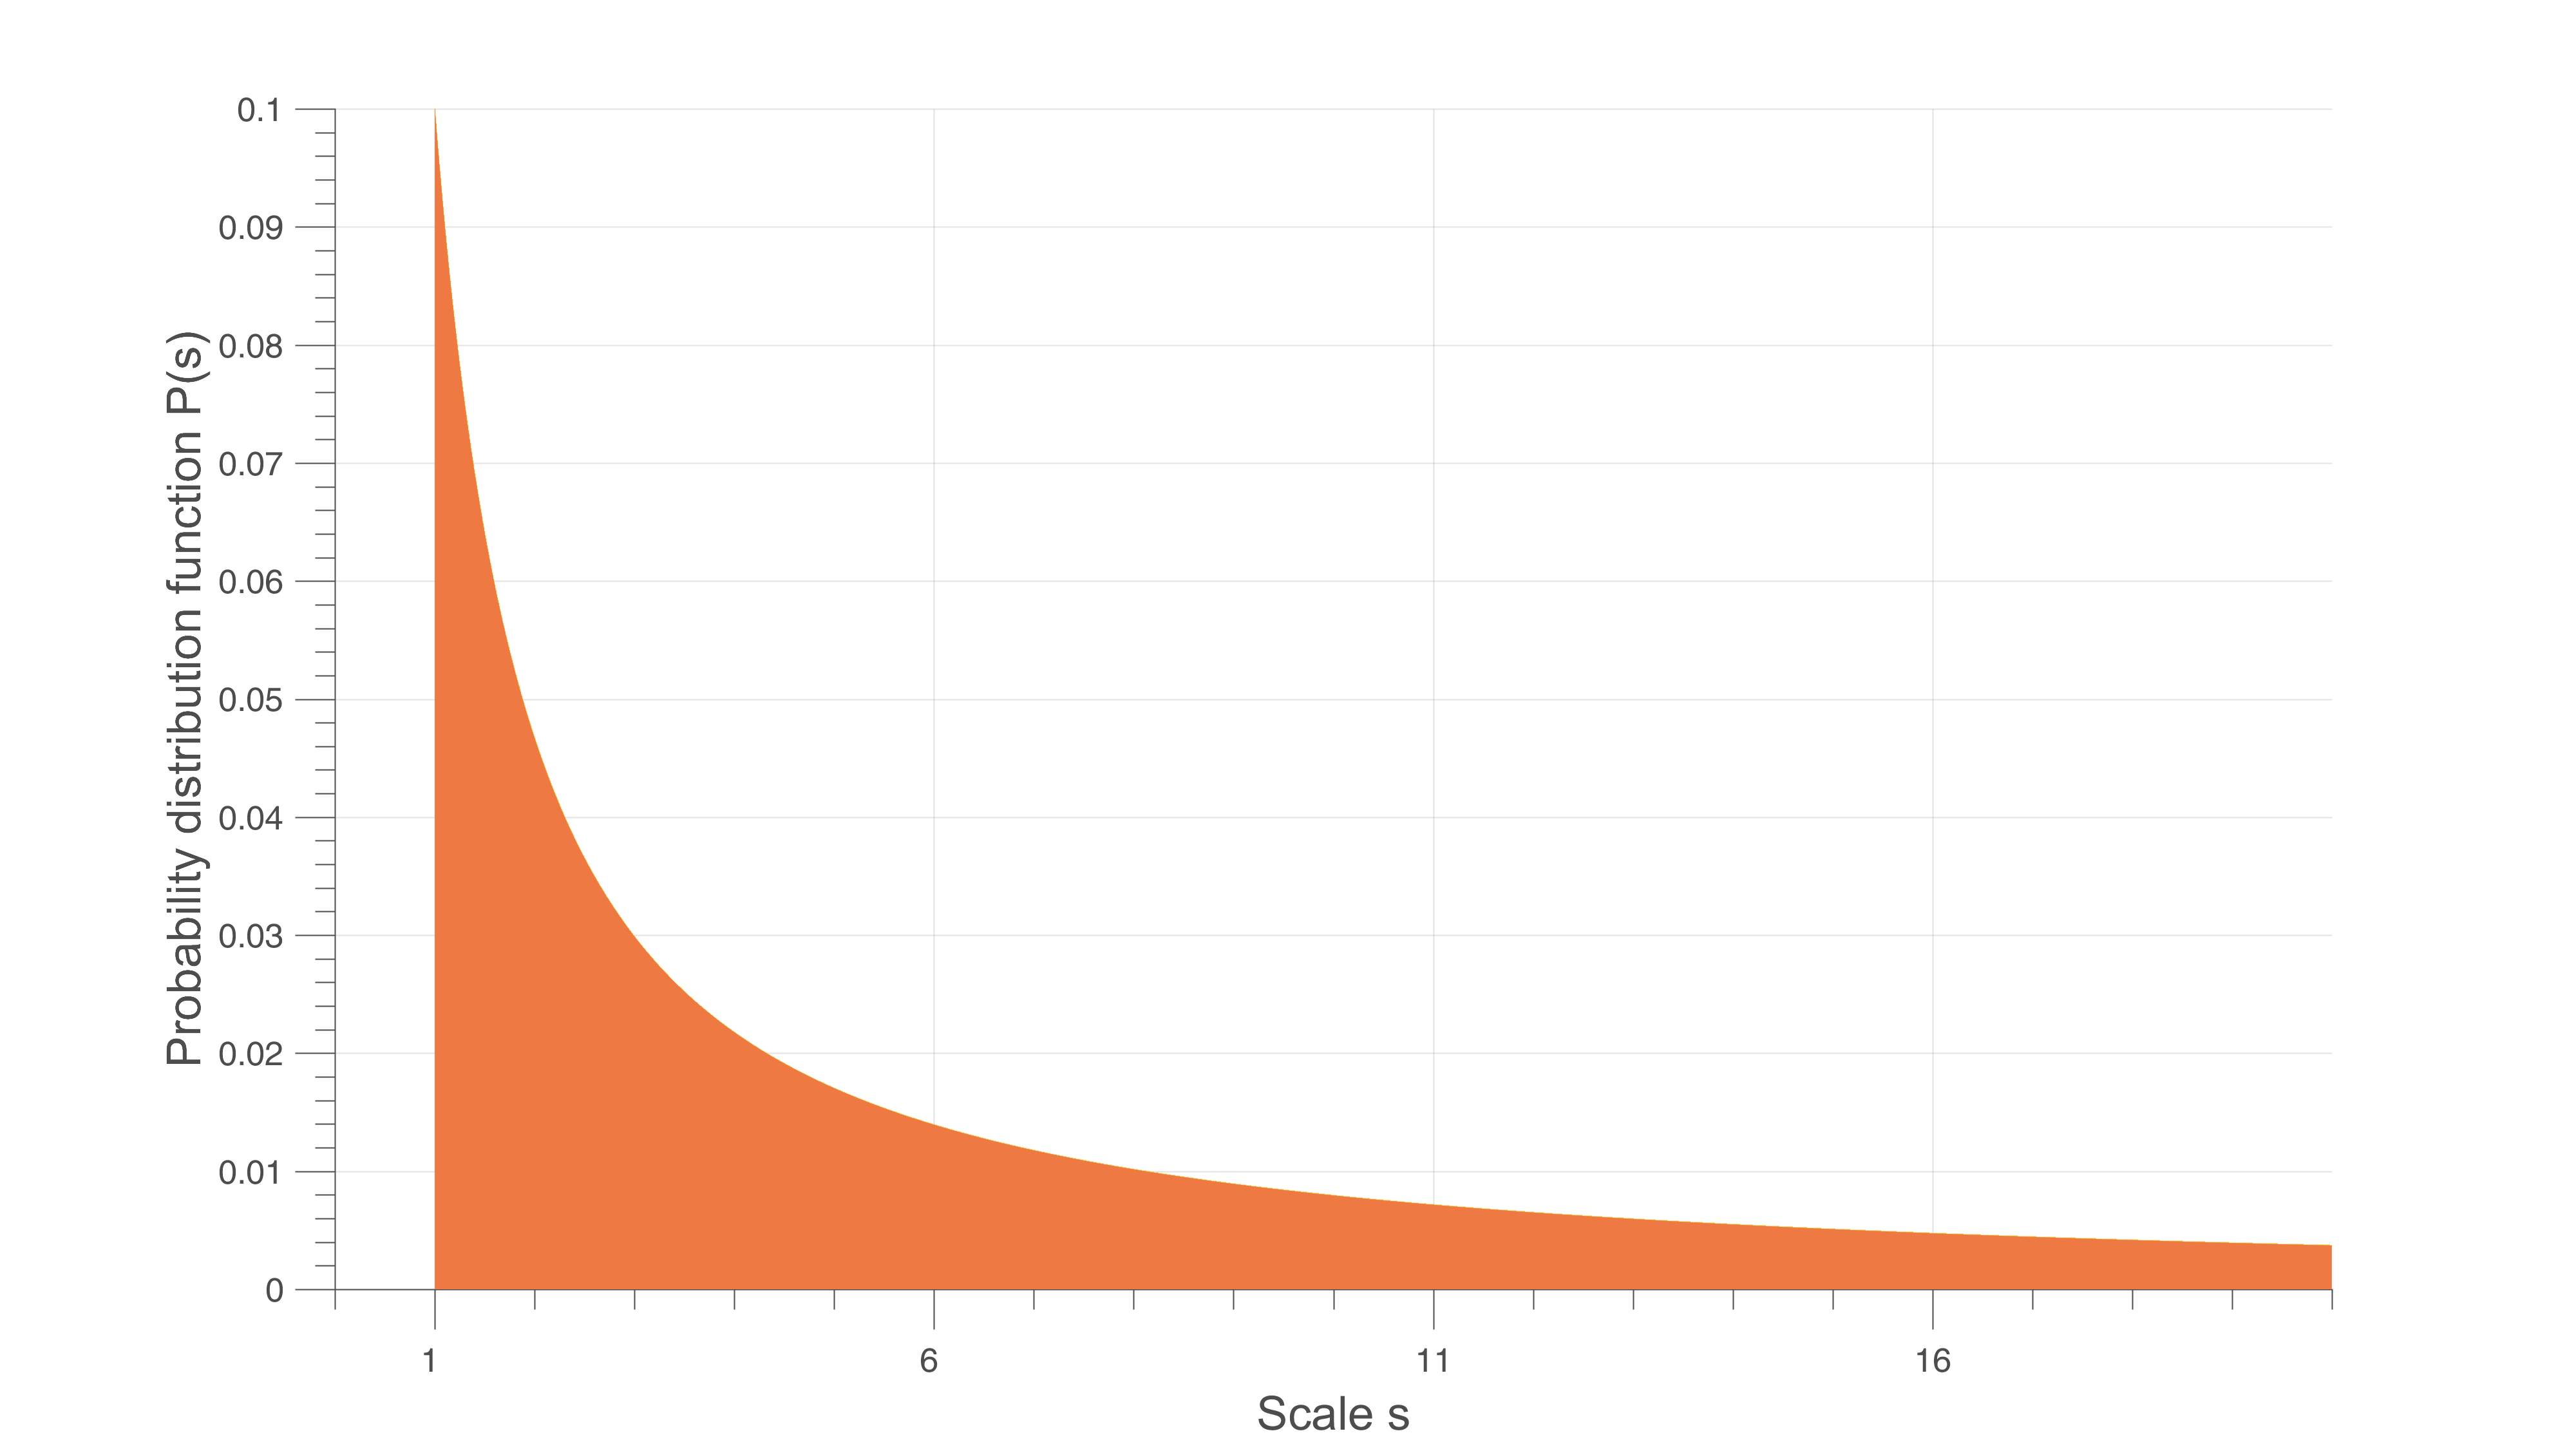
\includegraphics[width=0.9\textwidth]{figures//ps1.png} 
	\caption{Weakening scales $s$ probability distribution curve when $\beta=1.5$ }
	\label{ps1}
\end{figure}
\begin{figure}[!h]
	\centering
	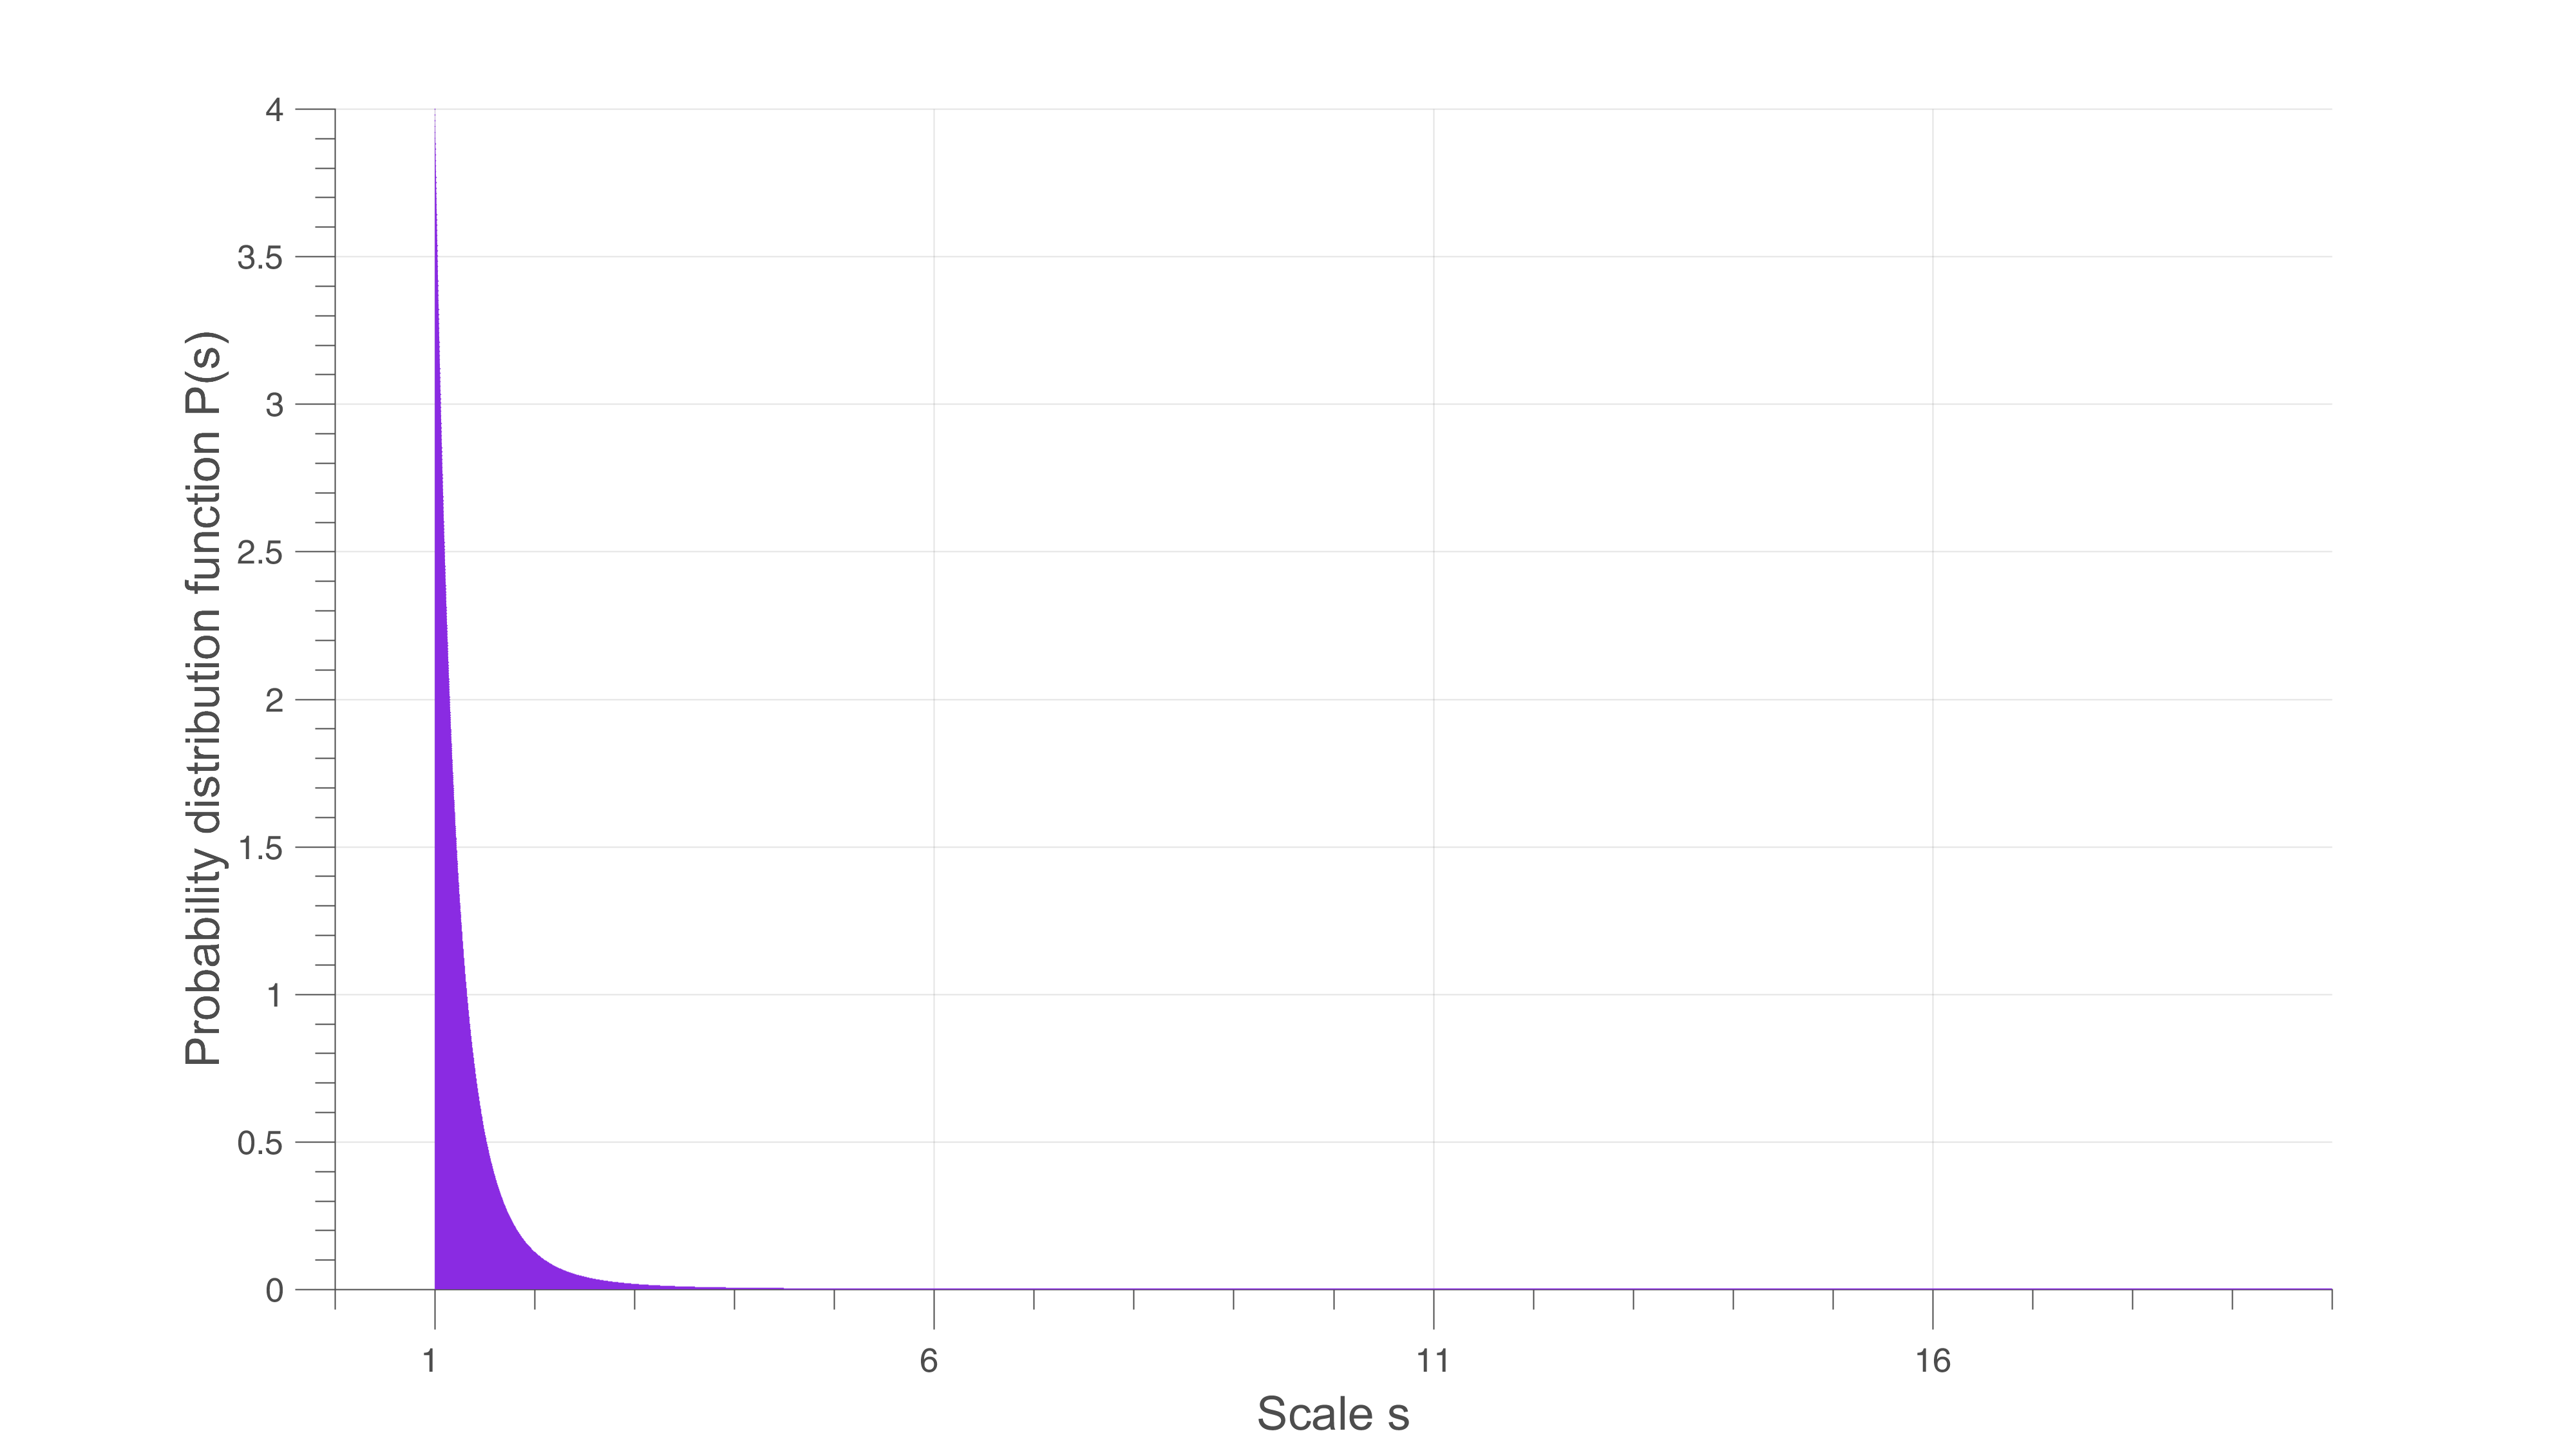
\includegraphics[width=0.9\textwidth]{figures//ps2.png} 
	\caption{Weakening scales $s$ probability distribution curve when $\beta=5$ }
	\label{ps2}
\end{figure}

\subsection{Yield function with mean stress effect}

Positive mean stress clearly reduces the fatigue life of the material. In design evaluation of multiaxial fatigue with mean stress, a simplified, conservative relation between mean stress and equivalent alternating stress is necessary. We can improve the model by modifying the yield function $\sigma_y$ and the localization tensor.

The idea is to consider as in Maitournam and Krebs\cite{Maitournam2011232} that the yield limit $\sigma_y$ can be reduced in presence of positive mean stress. The mesoscopic yield function can therefore be written as:
\begin{equation}
f\left(s\right)=||\uline{\uline{S}}(s)-\uline{\uline{b}}(s)||+\left( \lambda \Sigma_H-\sigma_y\right) /s\leqslant 0
\label{yieldfun}
\end{equation}
with $\uline{\uline{S}}$ denoting the deviatoric part of the stress tensor at microscale, and $\uline{\uline{b}}(s)$ the corresponding backstress at the same scale. The material remain in elastic regime when $f<0$ and in plastic regime when $f=0$.

\subsection{Local plastic model}
First we should describe the mesoscopic stress state.  The model considers a plastic 
behavior at the mesoscopic scale. The mesoscopic stress evolution equations are thus:

% \begin{numcases}{}
% 	\dot{\uline{\uline{S}}}(s,M,t)=dev\dot{\uline{\uline{\Sigma}}}(M,t)-\dfrac{E}{1+\nu}\dot{\uline{\uline{\varepsilon}}}^p(s,M,t), & Taylor-Lin scale transition model with unit localization tensor\cite{Bosia201239}.\\
% 	\dot{\uline{\uline{b}}}(s,M,t)=\dfrac{kE}{E-k} \dot{\uline{\uline{\varepsilon}}}^p(s,M,t) , & kinematic hardening model.\\
% 	\dot{\uline{\uline{\varepsilon}}}^p(s,M,t)=\gamma\dfrac{\partial f(s,M,t)}{\partial \uline{\uline{S}}}, & plastic flow rule assuming $\gamma=0$ when $f<0$ and  $\gamma\geqslant0$ when $f=0$.
% \end{numcases}
 
	\begin{equation}
    \dot{\uline{\uline{S}}}(s,M,t)=dev\dot{\uline{\uline{\Sigma}}}(M,t)-\dfrac{E}{1+\nu}\dot{\uline{\uline{\varepsilon}}}^p(s,M,t), 
	\end{equation}
     which defines a Taylor-Lin scale transition model with unit localization tensor\cite{Bosia201239}.
		\begin{equation}
		\dot{\uline{\uline{b}}}(s,M,t)=\dfrac{kE}{E-k} \dot{\uline{\uline{\varepsilon}}}^p(s,M,t), 
		\end{equation}
		which is our kinematic hardening model.
		\begin{equation}
		\dot{\uline{\uline{\varepsilon}}}^p(s,M,t)=C\dfrac{\partial f(s,M,t)}{\partial \uline{\uline{S}}}, 
		\end{equation}
		which is the associated plastic flow rule assuming $C=0$ when $f<0$ and  $C\geqslant0$ when $f=0$.

Here E denotes the Young's modulus and k the hardening parameter. The local dissipated energy rate per volume at weakening scales $s$  is given by the local entropy dissipation:
\begin{equation}
	\dot{w}(s,M,t)=(\uuline{S}-\uuline{b})(s,M,t):\uuline{\dot{\varepsilon}}^p(s,M,t).
	\label{dissipated}
\end{equation}

\section{Construction of an energy based fatigue approach}

In a preliminary step, we will consider a simple macroscopic loading history $\uuline{\Sigma}(M, t)$ which is uniaxial
and time periodic of deviatoric amplitude $S_{max}$, and a Von Mises flow rule to see if we get a prediction of local failure for a number of cycles $N_F$ varying as $\Sigma^{-\beta}.$


\noindent
In uniaxial cyclic loading, there will be 3 kinds of loading patterns, as is shown in \figref{backstress}:

\vspace{6pt}
\begin{enumerate}
	
	\item	Elastic regime, in phase 2 and 4,where $\dot{\uline{\uline{\varepsilon}}}^p(s,M,t)=0$ ,  and $|\uline{\uline{S}}-\uline{\uline{b}}|< \left( \sigma_y-\lambda \Sigma_H\right)/s. $ 
	\vspace{6pt}
	
	\item Plastic regime according to plastic flow rule, with increasing plastic deformation, in phase 5 and 1, where	$\dot{\uline{\uline{\varepsilon}}}^p(s,M,t)=C\dfrac{\uline{\uline{S}}(s)-\uline{\uline{b}}(s)}{||\uline{\uline{S}}(s)-\uline{\uline{b}}(s)||}> 0$ with  $C= dev\dot{\uline{\uline{\Sigma}}}\left(\dfrac{kE}{E-k}+\dfrac{E}{1+\nu} \right) ^{-1}$ ,  with $\uline{\uline{S}}-\uline{\uline{b}}= \left(\sigma_y-\lambda \Sigma_H\right)/s$ and $\dot{\uline{\uline{S}}}-\dot{\uline{\uline{b}}}=0.$ 
	\vspace{6pt}
	
	\item Plastic regime in the other direction, in phase 3, there is	$\dot{\uline{\uline{\varepsilon}}}^p(s,M,t)<0$,  then $\uline{\uline{S}}-\uline{\uline{b}}=- \left(\sigma_y-\lambda \Sigma_H\right)/s$ and $\dot{\uline{\uline{S}}}-\dot{\uline{\uline{b}}}=0$ 
	
\end{enumerate}	

\begin{figure}[!h]
	\centering
	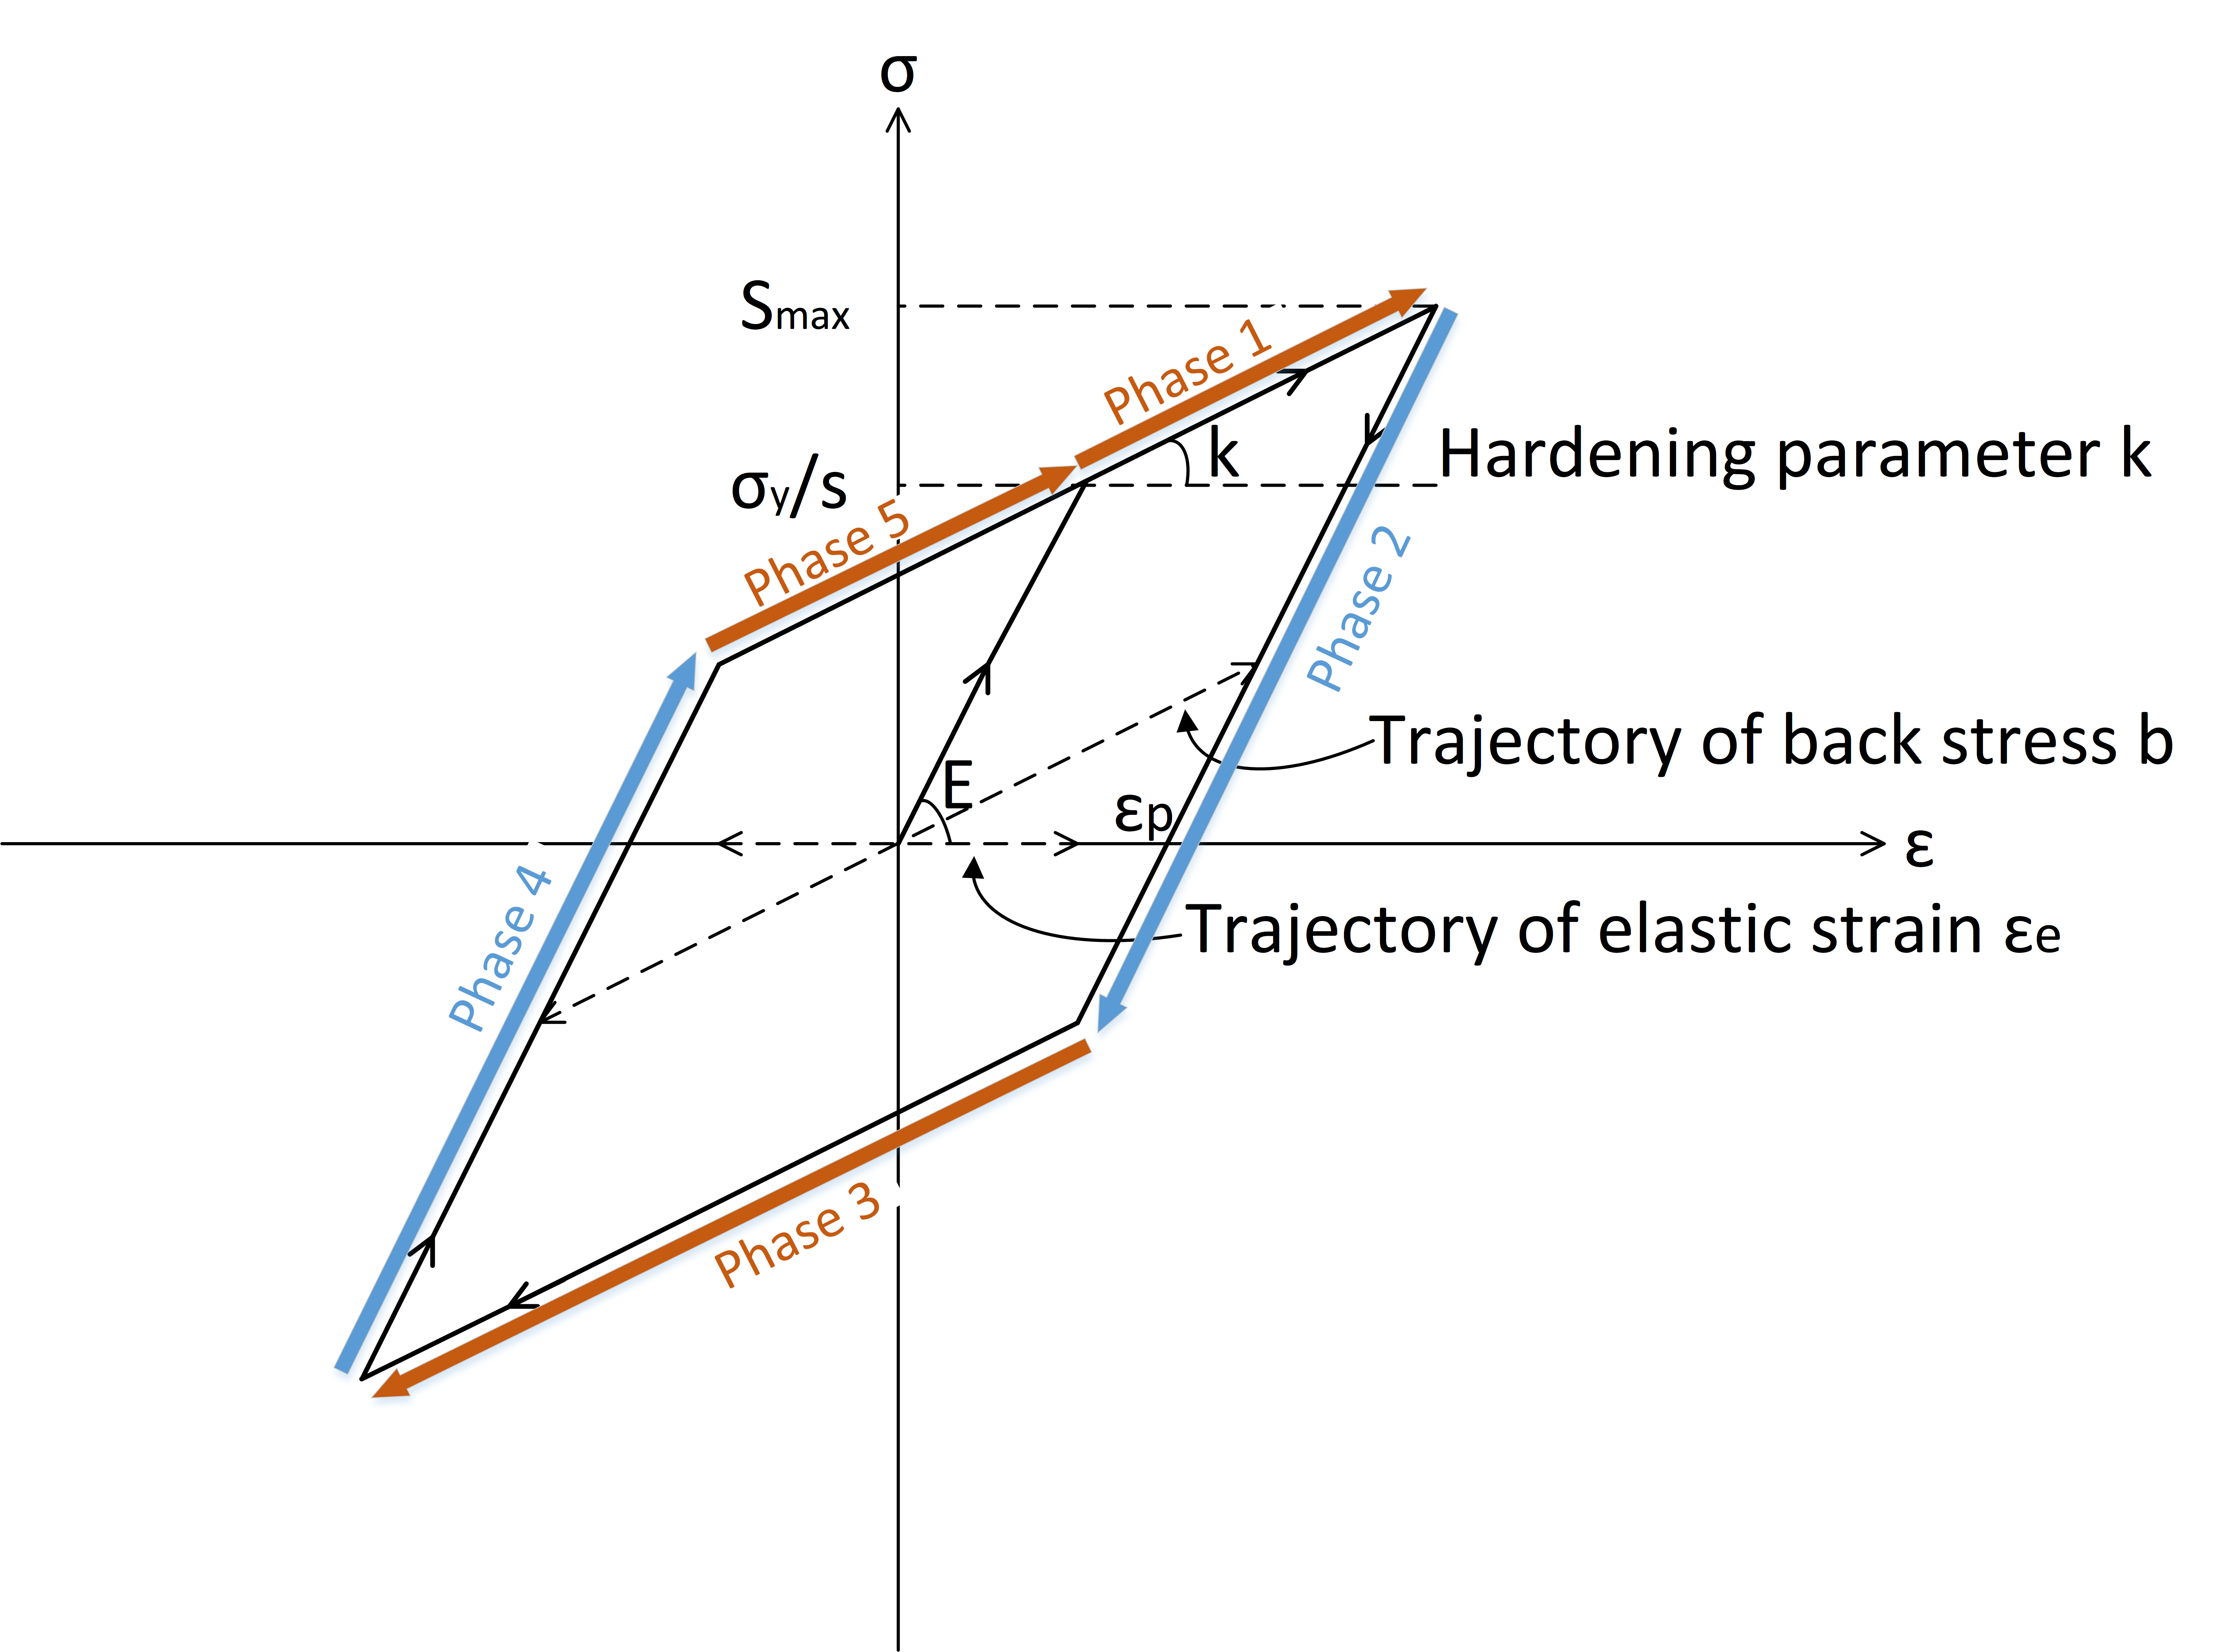
\includegraphics[width=0.9\textwidth]{figures//backstress.png} 
	\caption{Uniaxial load with plastic dissipation}
	\label{backstress}
\end{figure}

In phase 1, a direct analysis yields the energy dissipation at scale $s$:
\begin{equation}dW=(S-b)d\varepsilon^p=\dfrac{(E-k)(1+\nu) }{E(E+k\nu)}\dfrac{ \left(\sigma_y-\lambda \Sigma_H\right)}{s}\left(S_{max}-\dfrac{ \left(\sigma_y-\lambda \Sigma_H\right)}{s}\right)
\label{dw}
\end{equation}

A similar analysis yields $$dW(phase 1)=dW(phase 5)=\dfrac{1}{2}dW(phase 3).$$

We can then calculate  the local dissipated energy $W$  at point $M$ during one cycle by cumulating the input of all sub-scales which result in plastic regime with their probabilities \cite{zepeng}.
\begin{equation}
\begin{split}
W_{cyc}&=4\int_{ \left(\sigma_y-\lambda \Sigma_H\right) /S_{max}}^{\infty}dW(s,M,t)P(s)ds
\\&=4\int_{ \left(\sigma_y-\lambda \Sigma_H\right) /S_{max}}^{\infty}\dfrac{(E-k)(1+\nu) }{E(E+k\nu)}\dfrac{ \left(\sigma_y-\lambda \Sigma_H\right)}{s}\left(S_{max}-\dfrac{ \left(\sigma_y-\lambda \Sigma_H\right)}{s}\right)\left( \beta-1\right) s^{-\beta}ds
\\&=\dfrac{4(E-k)(1+\nu)\left( \beta-1\right) }{ E(E+k\nu)\beta\left( \beta+1\right) }\dfrac{S_{max}^{\beta+1}}{ \left(\sigma_y-\lambda \Sigma_H\right)^{\beta-1}}.
\end{split}
\label{eq:w}
\end{equation}

So we have a power law relationship between stress intensity and the dissipated energy per cycle as Eq.\eqref{eq.wcyc}.
\begin{equation}
W_{cyc}=C_1S_{max}^{\beta+1},
\label{eq.wcyc}
\end{equation}
with 
$$C_1=f(\lambda,\beta)=\dfrac{4(E-k)(1+\nu)\left( \beta-1\right) }{ E(E+k\nu)\beta\left( \beta+1\right)\left(\sigma_y-\lambda \Sigma_H\right)^{\beta-1} }.$$
 If the dissipated energy accumulates linearly until a failure value $W_0$, we can get directly the number of cycles to failure from Eq.\eqref{eq.NFcyc}:
\begin{equation}
N_{F}=\dfrac{W_0}{W_{cyc}}=\dfrac{W_0}{C_1}S_{max}^{-\beta-1}.
\label{eq.NFcyc}
\end{equation}
As for the time to failure in cyclic loading, there is:
$$T_{F}=N_{F}t_{cyc}.$$
From Eq.\eqref{eq:w}, we then obtain that the model predicts as expected a power law dependence in function of $S_{max}$.
However, experiments shows that the damage or the energy accumulation of a material evolves non-linearly in time. We should introduce below a method to handle such a nonlinearity.

\section{Nonlinearity of damage accumulation}
\subsection{Energy approach with Chaboche law}
The Chaboche law\cite{lemaitre1990mechanics} is essentially a damage incremental law for cyclic loading of stress intensity $\sigma$ with a deviatoric part ${A}_{\uppercase\expandafter{\romannumeral2}}$ and hydrostatic part $\Sigma_H$, defining the damage increase by:

 \begin{equation}\delta D = \left( 1 -(1-D)^{\gamma+1}\right)^\alpha \left(\frac{{A}_{\uppercase\expandafter{\romannumeral2}} }{M(\sigma_H)\left( 1-D\right)}\right)^\gamma \delta N
 \label{chabochemulti}
 \end{equation} 
 
With ${A}_{\uppercase\expandafter{\romannumeral2}}^*={A}_{\uppercase\expandafter{\romannumeral2}}/\left( 1-D\right) $ evolving with damage $D$. And the mean stress effect is in both exponential $\alpha$ and denominator $M(\sigma_H)$.
$$\alpha=1 - a\left\langle \dfrac{\dfrac{1}{2}J_2(t)-\sigma_{-1}M(\sigma_H) }{\sigma_{u} -J_2(t)}\right\rangle,$$
$$M(\sigma_H) =M_0 \left(1-3c\sigma_{H,max}(t) \right).$$
 
Eq.\eqref{chabochemulti} writes equivalently as Eq.\eqref{integration}:
   \begin{equation}\delta [1-(1-D)^{\gamma+1}]^{1-\alpha}=(1-\alpha)(\gamma+1)\left(\dfrac{{A}_{\uppercase\expandafter{\romannumeral2}} }{M(\Sigma_H)}\right)^\gamma \delta N=\dfrac{1}{N_F(\sigma)}\delta N.
   \label{integration}
   \end{equation}
Here $N_F(\sigma)$ denotes the number of cycles at intensity $\sigma$ to failure as obtained by integration of Eq.\eqref{integration} from $D=0$ to $D=1$. In our model, in case of a simple uniaxial cyclic loading, we propose to replace $\dfrac{1}{N_F(\Sigma)}$ which is the relative unit increment of energy by $\dfrac{W_{cyc}(\Sigma)}{W_0}$.



The nonlinear damage incremental law using energy dissipation:
\begin{equation}
\begin{split}
  \delta D &=\dfrac{\left( 1 -(1-D)^{\gamma+1}\right)^\alpha}{\left(1-D \right)^\gamma} \delta W
  \\&= \dfrac{\left( 1 -(1-D)^{\gamma+1}\right)^\alpha}{\left(1-D \right)^\gamma} \dfrac{W_{cyc}\delta N}{W_0}
  \\&= \dfrac{\left( 1 -(1-D)^{\gamma+1}\right)^\alpha}{\left(1-D \right)^\gamma} \dfrac{4(E-k)(1+\nu)\left( \beta-1\right) }{ E(E+k\nu)\beta\left( \beta+1\right) }\dfrac{S_{max}^{\beta+1}}{\left(\sigma_y-\lambda \Sigma_H\right)^{\beta-1}}\dfrac{\delta N}{W_0}.
\end{split}
\label{recoverchaboche}
\end{equation} 

We compare Eq.\eqref{chabochemulti} and Eq.\eqref{recoverchaboche}, in Chaboche model there is:
$$\beta+1=\gamma. $$

Similar to Eq.\eqref{integration}, we define here the ``equivalent damage'' $\tilde{D}$ in Eq.\eqref{eq.Dhat}:

\begin{equation}
\tilde{D}=1-(1-D)^{\gamma+1},
\label{eq.Dhat}
\end{equation}
with $D$ the damage variable introduced by Chaboche in its model to scale the stress intensity:
$${A}_{\uppercase\expandafter{\romannumeral2}} \longrightarrow \dfrac{{A}_{\uppercase\expandafter{\romannumeral2}}}{1-D}.$$

We have 

$\bullet$ $\tilde{D}=0$ when $D=0$(undamaged material),

$\bullet$ $\tilde{D}=1$ when $D=1$(failure of material),	

and a nonlinear relation in between as in \figref{fig.Dhat}:
$$\delta\tilde{D}=\left(\gamma+1 \right)\left( 1-D\right)^\gamma \delta D.$$	
\begin{figure}
	\centering
	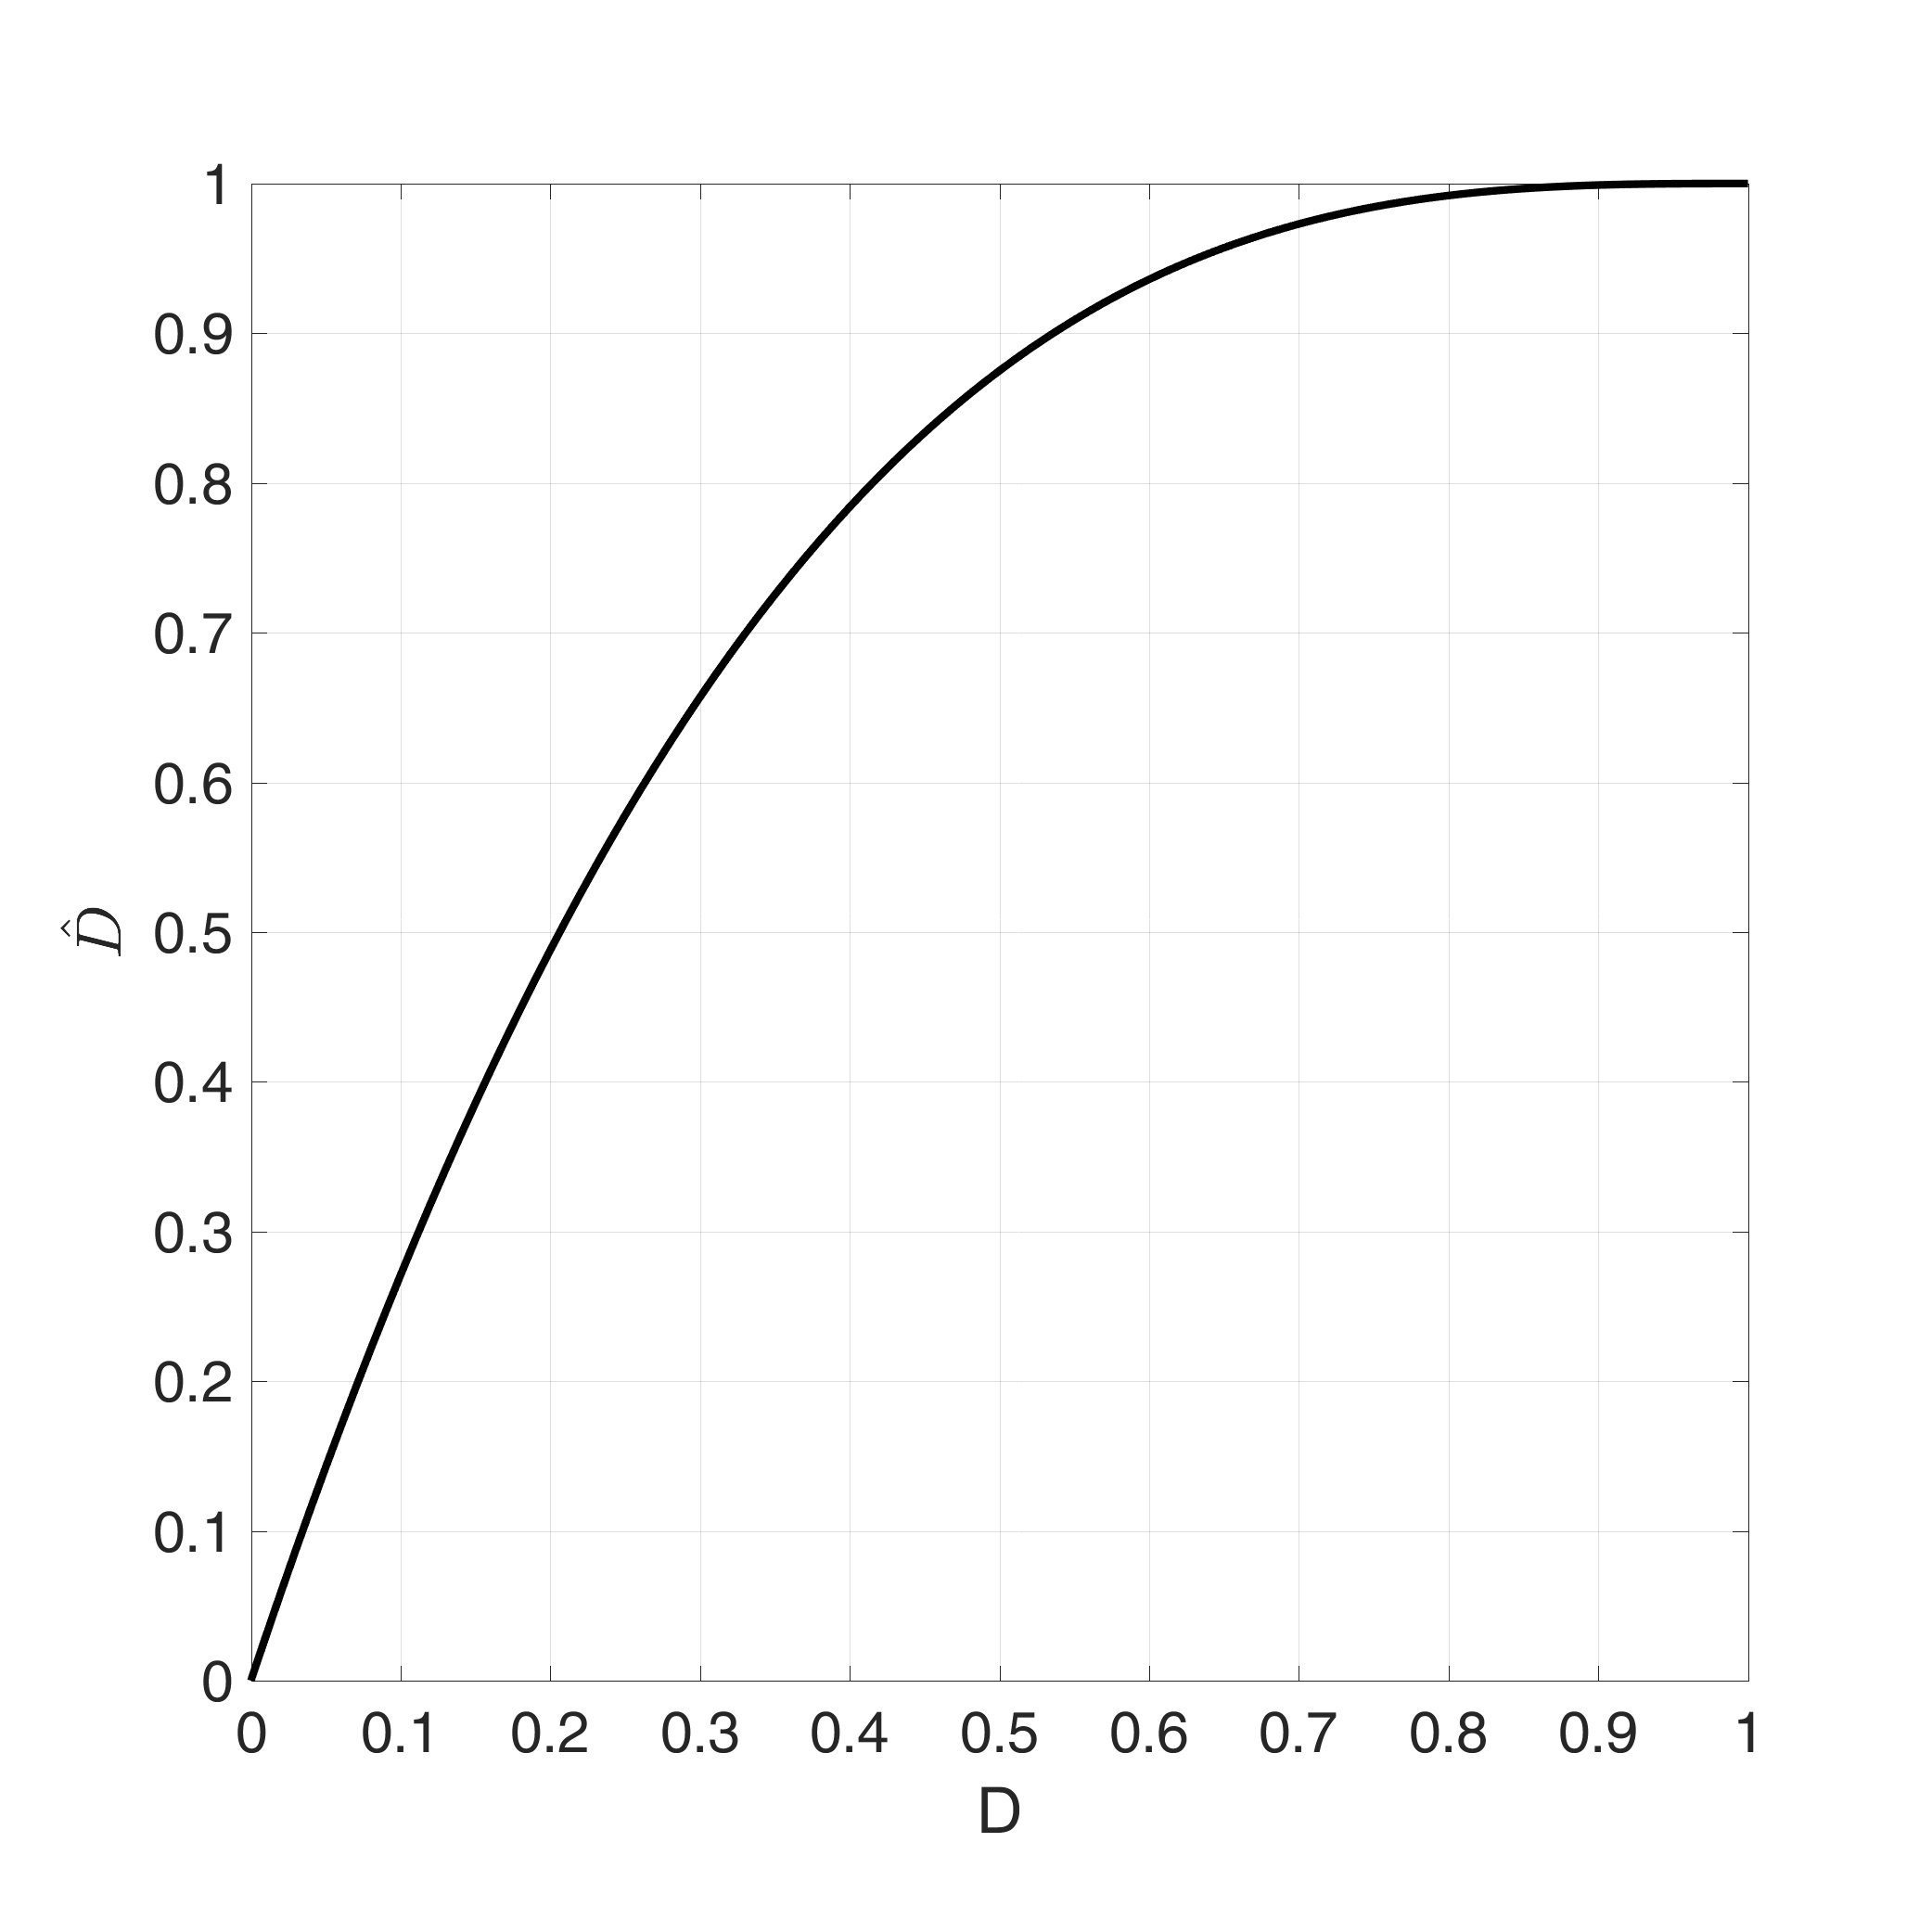
\includegraphics[width=0.5\textwidth]{figures//Dhat.png} 
	\caption{The relation between $\tilde{D}$ and $D$ when $\gamma=2$}
	\label{fig.Dhat}
\end{figure}

Change of damage measure $\tilde{D} = 1 - (1-D)^{\gamma+1}$ makes the law explicit. The differential equation
$
\dfrac{d\tilde{D}}{dN} = c_D {\tilde{D}}^\alpha J_2^\gamma
$
predicts a number of cycles to fatigue at constant load is given by
$$
N_F =c_N \frac{1}{1-\alpha} J_2^\gamma.
$$

This method requires cycle counting witch is difficult and technical for complex load histories. In addition, it has limited influence of multiaxiality.


Now in our model we use the same growth rule as in Chaboche in cyclic load regime, but replace stress intensity by multiscale dissipated energy (no cycle counting) in Eq.\eqref{eq.DWcyc}.

$$
\dfrac{d\tilde{D}}{dN} =c_D {\tilde{D}}^\alpha J_2^\gamma \to \dfrac{d\tilde{D}}{dt} ={\tilde{D}}^\alpha \dot{W}/W_0.
$$

\begin{equation}
\delta \tilde{D}=\tilde{D}^\alpha\dfrac{\delta W}{W_0}=\tilde{D}^\alpha\dfrac{W_{cyc}\delta N}{W_0}.
\label{eq.DWcyc}
\end{equation}

The number of cycles to failure in constant loading case, obtained by integrating $D$ from 0 to 1 is:
\begin{equation}
N_F=\dfrac{W_0}{\left( 1-\alpha\right)W_{cyc} }=\dfrac{W_0}{\left( 1-\alpha\right)C_1}S_{max}^{-\beta-1}.
\label{eq.NFWcyc}
\end{equation}
 
From Eq.\eqref{eq.NFWcyc}, we see $(-\beta-1)$ is related to the slop in S-N curve and $\dfrac{W_0}{C_1}$ defines the number of cycles to failure.
 
 
\subsection{Generalized damage accumulation}
Eq.\eqref{integration} is a general accumulation law which can be applied for any cyclic loading sequence provided that we can identify the multiscale value of the dissipated energy per cycle. 

But the notion of cycle itself may be hard to identify for general loadings. The idea is then to replace the relative increment of dissipated energy per cycle by the relative increment of dissipated energy per unit time, yielding Eq.\eqref{eq.DW}:
\begin{equation}
\delta\tilde{D}= \tilde{D}^\alpha \dfrac{W}{W_0} = \tilde{D}^\alpha \dfrac{\dot{W}\delta t}{W_0}
\label{eq.DW}
\end{equation}
giving equivalent differential form of damage accumulation:
\begin{equation}
\label{eq.DW2}
\end{equation}
The time to failure, obtained by integrating $\tilde{D}$ from 0 to 1 is:
\begin{equation}
T_F = \frac{1}{1-\alpha}\dfrac{W_0}{\dot{W}}.
\label{eq.tf}
\end{equation}

In differential form, the relation \eqref{eq.diffform} writes from Eq.\eqref{eq.DW} and Eq.\eqref{eq.tf}:
\begin{equation}
\delta \tilde{D}^{1-\alpha}=\frac{\delta t}{T_F}.
\label{eq.diffform}
\end{equation}

When we integrate Eq.\eqref{eq.DW} from $0$ to $\tilde{D}$ at constant loading conditions. The damage, expressed as a function of $t/T_F$ is:
\begin{equation}
\tilde{D}=\left( \frac{t}{T_F}\right) ^{\frac{1}{1-\alpha}}.
\label{eqD}
\end{equation}
This expression is in good agreement with experimental results\cite{lemaitre1990mechanics}. 

In a general loading case, $\dot{W}$ is the microscopic energy dissipation rate of unit defect and $W_0$ is the energy threshold of unit defect. By integrating Eq.\eqref{dissipated} over all microscales, we get:
\begin{equation}\dot{W}(M,t)=\int_{s=1}^{\infty}\dot{w}(s,M,t)P(s)ds=\int_{s=1}^{\infty}\left(\uuline{S}-\uuline{b} \right) (s,M,t):\uuline{\dot{\varepsilon}^p}(s,M,t)P(s)ds.\label{Wdot}
\end{equation}
The evolution of $\uuline{S}$, $\uuline{b}$ and $\uuline{\dot{\varepsilon}}^p$ are given previously. Eq.\eqref{eq.DW} and \eqref{Wdot} are therefore our proposed damage incremental law with energy dissipation.

This is a nonlinear law with a constant $\alpha$, there will be no sequence effect. In other words,
when applying two successive cycles of different intensities, the failure will occur at the same number of cycles whatever the order of the loading(high then low versus low then high). In numerical implementation of complex loading case, to take into account the load sequence effect, $\alpha$ changes at every time step.

We introduce $s_{min}$, which is the minimum scale that causes energy loss:
\begin{equation}
s_{min}=\dfrac{\left(\sigma_y-\lambda \Sigma_H\right)}{S_{max}}.
\label{eq.smin}
\end{equation}
To take into account the sequence effect, the parameter $\alpha$ should change with $S_{max}$ in order to handle change of cycle intensity and the influence on fatigue life.

\subsection{Sequence effect}

Experiments show fatigue tests started with high stress then change to low stress has less fatigue life than the combination of high stress life proportion plus the low one. This phenomenon of sequence effect is load history dependent, so we need a stress induced parameter to describe it. 

This is done in Chaboche  with three ingredients:

\begin{enumerate} 
	\vspace{6pt}
	\item Notion of damage sensitive effective stress: 
	$$\sigma_D^{eff} = J_2(\uline{\uline{\Sigma}})/(1-D)$$.
	
	\vspace{6pt}
	
	\item $(\sigma_D^{eff})^\gamma$ controlled  law for damage growth
	$$
	\dfrac{dD}{dN} =c_\gamma {\tilde{D}}^\alpha (\sigma_D^{eff})^\gamma.
	$$
	
	\vspace{6pt}
	
	\item  Load dependence of exponent $\alpha$ (from $1$ at zero load to $0$ at large loads).
\end{enumerate}

Many fatigue damage accumulation models are based on the two level loading experiments which is one of the basic random loading analysis. To facilitate our verification of the law we use two-stress level loading, the specimen is firstly loaded at stress $\Sigma_1$ for $T_1$ cycles and then at stress $\Sigma_2$ for $T_2$ cycles until failure. We can then observe if the experimental results are satisfactory.

In Chaboche model, the proposition of $\alpha$ is:

\begin{equation}
\alpha = 1 - a\left\langle \frac{ \sigma_{eq}-\sigma_{fatigue}}{ \sigma_{u} - \sigma_{eq}}\right\rangle.
\end{equation}

We propose a load dependent $\alpha$ through $s_{min}$ (= the smallest scale experiencing plastic dissipation). Possible choice
 of $\alpha$ is expressed as Eq.\eqref{eq.alpha}:
\begin{equation}
\alpha=1-a\left( \dfrac{\frac{1}{s_{min}}}{1-\frac{1}{s_{min}}} \right) .
\label{eq.alpha}
\end{equation}

There is no notion of fatigue limit in our model, $\sigma_{faigue}=0$. The intensity of loading
 $$\frac{ \sigma_{eq}-\sigma_{fatigue}}{ \sigma_{u} - \sigma_{eq}}= \frac{ 1}{\frac{\sigma_{u}}{\sigma_{eq}} -1}$$
 is measured by 
$$\left( \dfrac{\frac{1}{s_{min}}}{1-\frac{1}{s_{min}}}\right) =\left(s_{min}-1 \right) ^{-1}.$$
This means that we measure the distance of load to ultimate failure by local variable $s_{min}$ through 

$$\frac{\sigma_{u}}{\sigma_{eq}} -1 \longrightarrow \left( s_{min}-1\right)  $$


We have $T_F$ expressed in Eq.\eqref{eq.tf} and differential form of damage accumulation in Eq.\eqref{eq.DW2}. Now we are able ot chain two cycles $i=1$ and $i=2$  (at  rate $\dot{W}_i$ associated to exponent $\alpha_i$). Firstly after loading time $T_1$, we  cycle  from $\tilde{D}=0$ to $\tilde{D}= \tilde{D}_1$ by integrating Eq.\eqref{eq.diffform}:
\begin{equation}
\left( 1-\tilde{D}_1\right) ^{1-\alpha_1}=\dfrac{T_1}{T_{F1}}
\label{23a}
\end{equation}

then we cycle from  ${\tilde D}={\tilde D}_1$ to failure ${\tilde D}=1$:
\begin{equation}
1-\left( 1-\tilde{D}_1\right)^{1-\alpha_2}=\dfrac{T_2}{T_{F2}}
\label{23b}
\end{equation}

From Eq.\eqref{23a} and Eq.\eqref{23b}, after elimination of $\left( 1-D_1\right)$ we get:
\begin{equation} 
\dfrac{T_2}{T_{F2}} =1-\left( \dfrac{T_1}{T_{F1}}\right) ^\eta,
\end{equation}
with
\begin{equation}
\eta=\dfrac{1-\alpha_2}{1-\alpha_1}.
\label{eq.eta}
\end{equation}

In the case of high-low loading sequence there is $\Sigma_1>\Sigma_2$, meaning $S_{max1}>S_{max2}$, which gives $\alpha_1<\alpha_2$, so we have:
$$\eta=\frac{1-\alpha_2}{1-\alpha_1}<1 \implies
 \frac{T_2}{T_{F2}}=1-\left( \frac{T_1}{T_{F1}}\right) ^\eta<1-\frac{T_1}{T_{F1}} \implies
\frac{T_1}{T_{F1}}+\frac{T_2}{T_{F2}}<1.$$

We can see from \figref{fig.sequence} that cycling $1$ for fifty percent of its failure time leaves a reserve before failure to cycle $2$ much less than fifty percent. To conclude, the cumulative damage under high-low loading sequence, as we deduced, has the addition of partial lives less than unit. Similarly, the cumulative damage under low-high loading sequence has addition of partial lives more than 1.
$$\frac{T_1}{T_{F1}}+\frac{T_2}{T_{F2}}>1$$
 The curve is depicted in \figref{fig.sequence}.
\begin{figure}[!h]
	\centering
	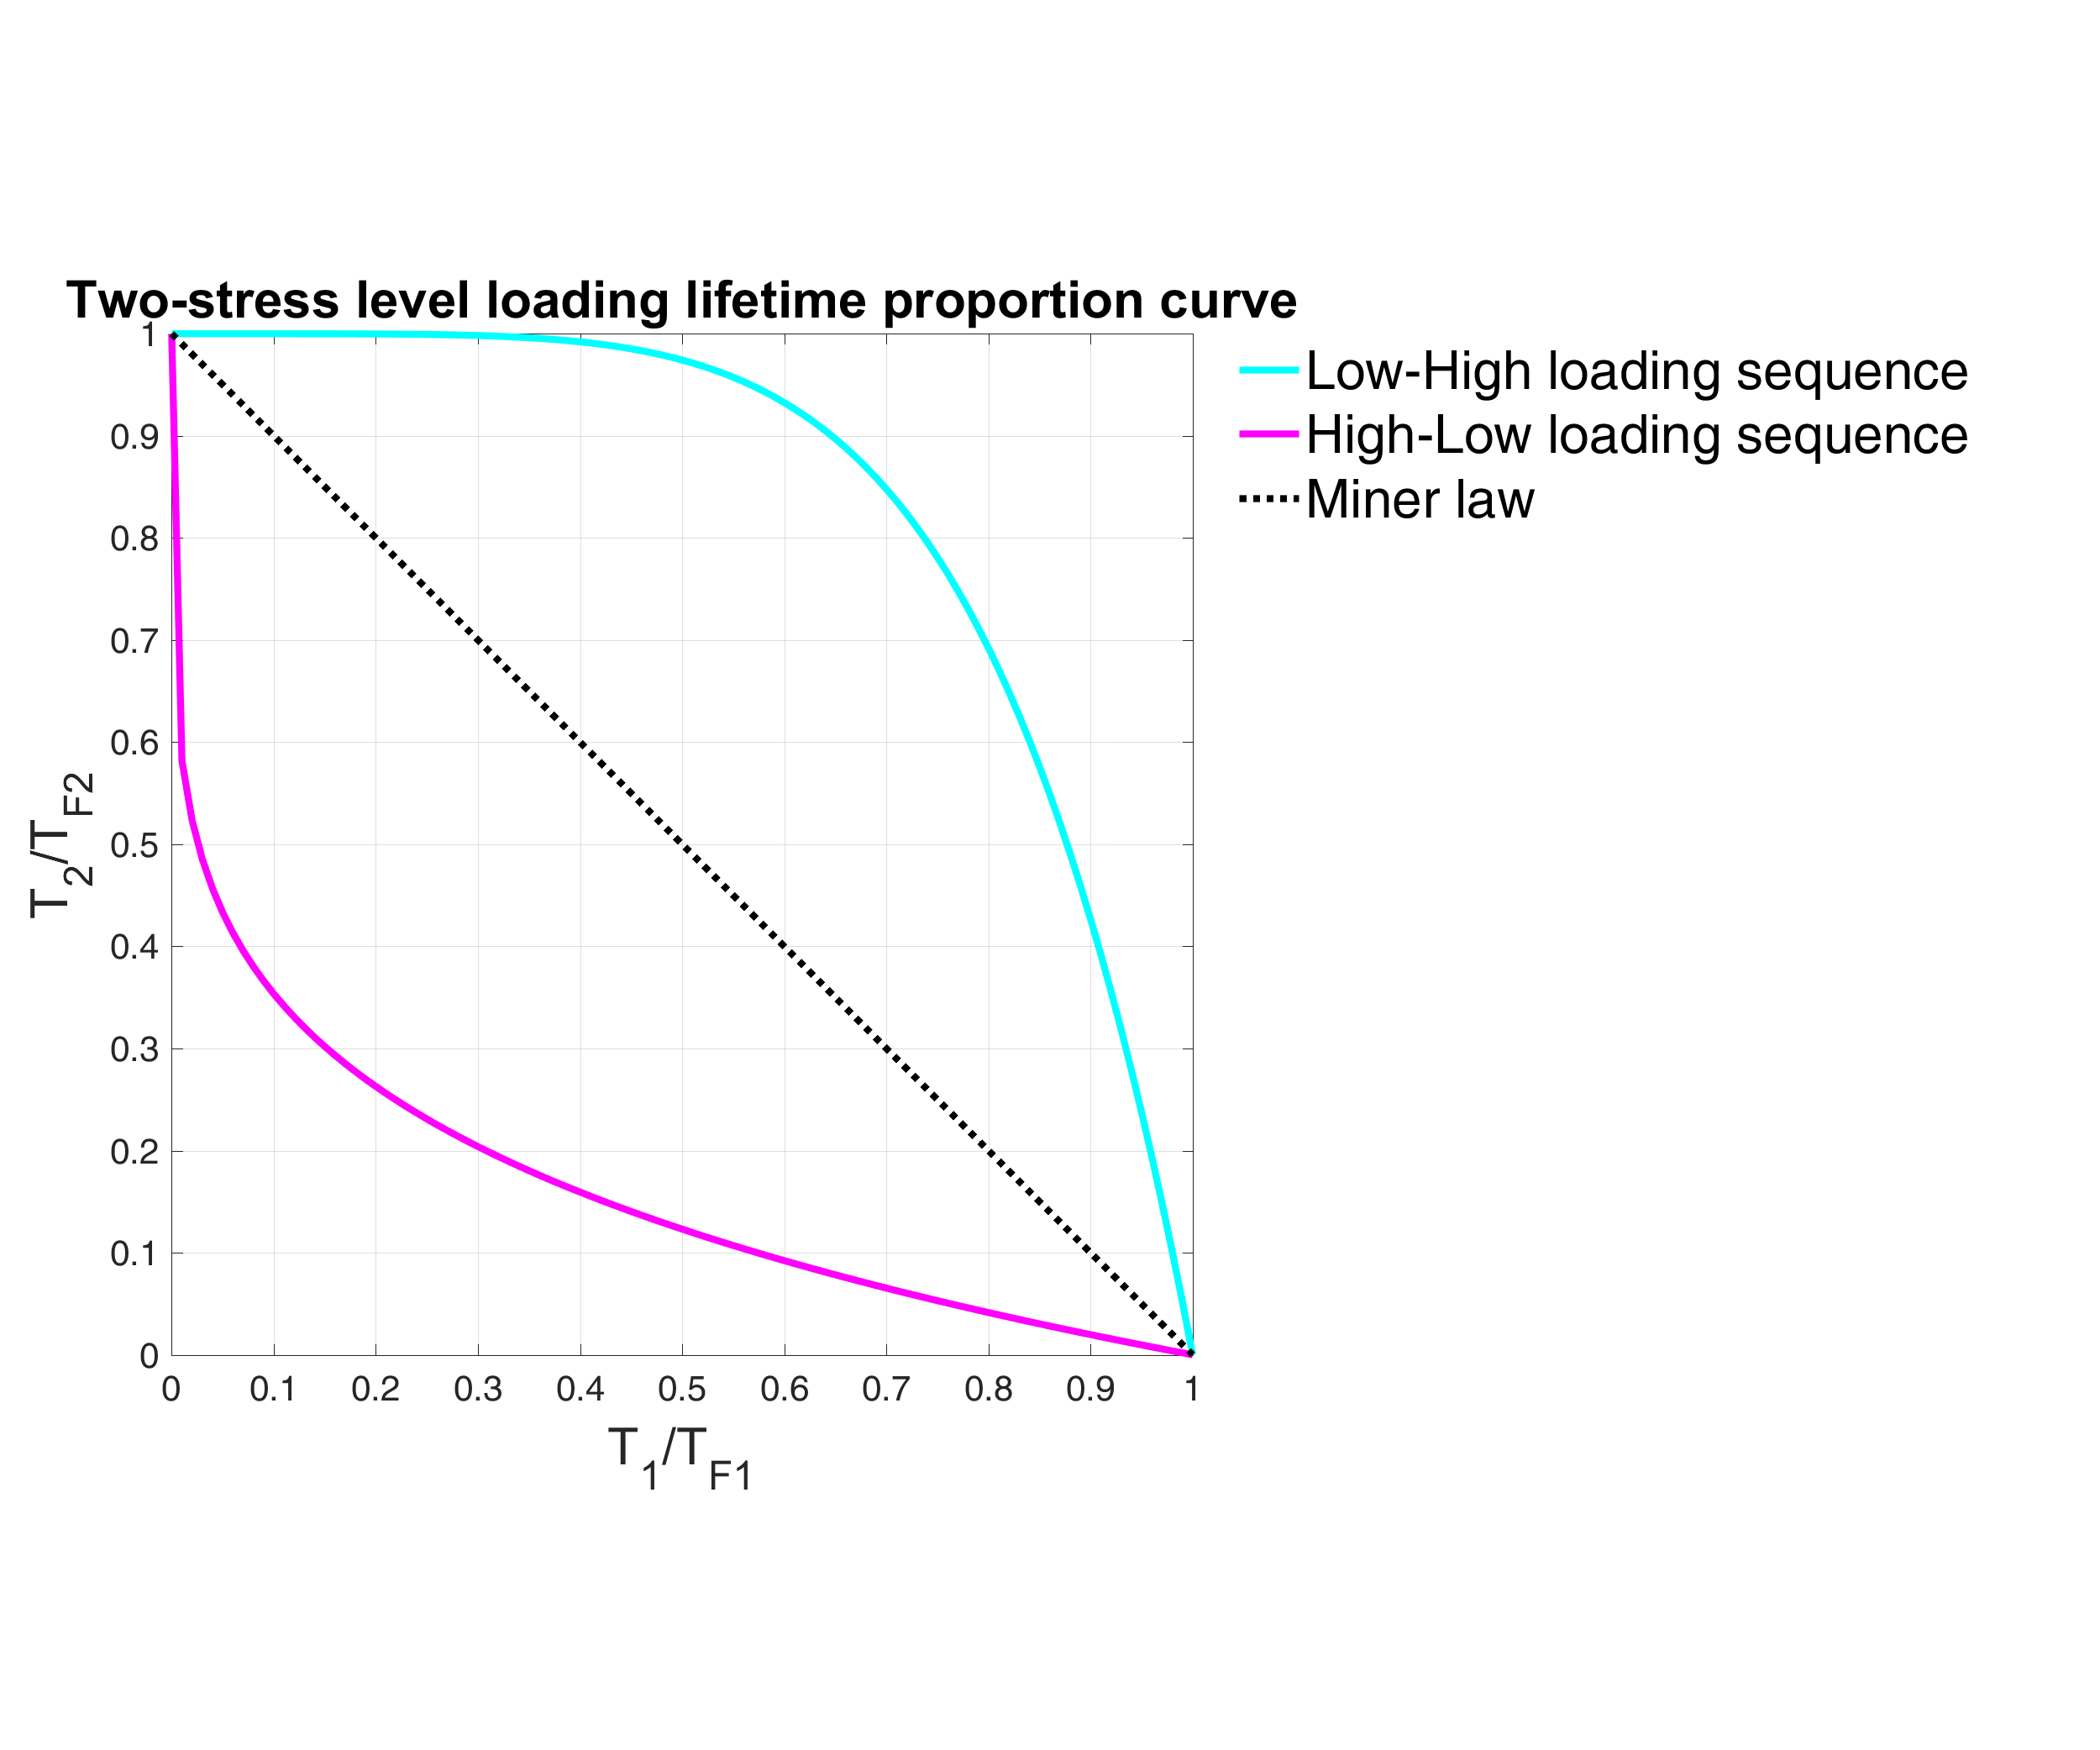
\includegraphics[width=\textwidth]{figures//sequence.png} 
	\caption{High to low and low to high loading sequence comparison}
	\label{fig.sequence}
\end{figure}
For constant two-level stress loading, $\alpha_1=\alpha_2$, the Chaboche law returns to the Miner rule where:
$$\frac{T_1}{T_{F1}}+\frac{T_2}{T_{F2}}=1$$

\newpage
\section{Numerical strategy}
\subsection{Integration rules for $\dot{W}$ and $\delta \tilde{D}$}
Our first approach takes one cycle as unit time. We compute analytically the energy dissipation at each scale during this cycle. The method is valid for simple loading history and which includes the integration on all weakening scales. The damage $\tilde{D}$ is accumulated after each cycle.

However, there are certain limitations of this method. Firstly we need a load history decomposition in cycles. Secondly in real life the perfect close loop cycle is hardly applicable.

Thus we propose in Eq.\eqref{eq.DW} a more general method which can be integrated by a step by step strategy. We compute numerically the dissipation at different scales using an implicit Euler time integration of the constitutive laws of section 1.4. After which we make a numerical integration on different scales. Then we can update the damage and go to next time step. 

Instead of doing the scale integration directly which can be difficult for complex loading, the Gaussian Quadrature rule with Legendre points is used to give the value of local dissipated energy rate.

To use the Gaussian quadrature rule the limit range of integral must be from $-1$ to $1$, while the total dissipated energy  is expressed by integrating all the weakening scale $s$ ranging from 1 to infinity with their occurrence probabilities:
$$\dot{W}=\int_{1}^{\infty}\dot{w}(s) (\beta-1)(s)^{-\beta}ds.$$

\noindent
To change the limit range of integral from $[1,\infty]$ to $[1,0]$ we take as new integration variable
$u(s)= s^{-p}$ with $p=\beta-1$, yielding $u(1)=1$ and  $u(\infty)=0$ with
$$du=-ps^{-p-1}ds$$ 
that is
$$du=(-\beta+1) s^{-\beta}ds=(-\beta+1)s^{-\beta} ds.$$
Therefore the dissipated energy summed on all scales is:
\begin{equation}
\begin{split}
\dot{W}&=\int_{1}^{\infty}\dot{w}(s) (\beta-1)(s)^{-\beta}ds
\\&=\int_{1}^{0}\dot{w}\left( u^{\frac{1}{1-\beta}}\right) (\beta-1) \frac{1}{-\beta+1}du
\\&=\int_{0}^{1}\dot{w}\left( u^{\frac{1}{1-\beta}}\right) (\beta-1) \frac{1}{\beta-1}du
\\&=\int_{0}^{1}\dot{w}\left( u^{\frac{1}{1-\beta}}\right)du
\\&=\frac{1}{2}\int_{-1}^{1}\dot{w}\left[  \left( \frac{x+1}{2}\right) ^{\frac{1}{1-\beta}}\right] dx
\end{split}
\label{allscale}
\end{equation}
given $u=\dfrac{x+1}{2}$.

So the dissipated energy rate integrated over all scales takes the form of Eq.\eqref{allscalerate}:
\begin{equation}
\dot{W}=\frac{1}{2}\int_{-1}^{1}\dot{w}\left[  \left( \frac{x+1}{2}\right) ^{\frac{1}{1-\beta}},t\right] dx\approx\frac{1}{2}\sum_{i}\omega_i\dot{w}\left[  \left( \frac{x_i+1}{2}\right) ^{\frac{1}{1-\beta}},t\right],
\label{allscalerate}
\end{equation}
where $\omega_i$ and $x_i$ are respectively the weights and nodes of the Gauss Legendre integration rule used for the numerical integration. The use of Gaussian Quadrature rule changes the integrand s from infinity to finite fixed values without affecting the integration results. In this work, we used 64 points\cite{legendre}.

After changing the integration limit, $\left( \dfrac{x+1}{2}\right) ^{\frac{1}{1-\beta}}$ represents the weakening scale $s$. 

Damage accumulation is deduced from Eq.\eqref{eq.DW}:
\begin{equation}
\tilde{D}_{n+1}=\tilde{D}_n+\tilde{D}_n^\alpha\dfrac{W}{W_0}
\label{eq.damage}
\end{equation}

with $W=\dot{W}dt$
We upgrade the damage step by step following Eq.\eqref{eq.damage}. When $\tilde{D}$ reaches one, the material fails. 

\subsection{Regime determination under multiple scales}
The material could be both in elastic and plastic regime at different scales. To be more elaborate, we reuse the fundamental equations in different regimes. At scale $s$, we have a dissipation rate given by:
$$\dot{w}(s)=\left( \uline{\uline{S}}-\uline{\uline{b}}\right):\dot{\uline{\uline{\varepsilon}}}^p, $$
which differs between plastic and elastic regime.

\vspace{6pt}
\noindent
\textbf{Elastic regime:}

\vspace{6pt}
\noindent
There we have
plastic strain rate
$\dot{\uline{\uline{\varepsilon}}}^p=0$, back stress rate $\dot{\uline{\uline{b}}}=0$ and deviatoric stress rate $\dot{\uline{\uline{S}}}=dev\dot{\uline{\uline{\Sigma}}}$, leading to
$$\dot{\uline{\uline{S}}}-\dot{\uline{\uline{b}}}=dev\dot{\uline{\uline{\Sigma}}},$$ 
meaning
$$\left( \uline{\uline{S}}-\uline{\uline{b}}\right) (t+dt)=\left( \uline{\uline{S}}-\uline{\uline{b}}\right) (t)+dev\dot{\uline{\uline{\Sigma}}}dt.$$
At each time step we define a trial stress:
\begin{equation}
\left( \uline{\uline{S}}-\uline{\uline{b}}\right)(t+dt):=\left( \uline{\uline{S}}-\uline{\uline{b}}\right)_{trial}.
\label{trial}
\end{equation}
We are in elastic regime at scale $s$ as long as we satisfy

$$\left( \uline{\uline{S}}-\uline{\uline{b}}\right)_{trial}\leqslant\left( \sigma_y-\lambda \Sigma_H\right)/s  $$

\vspace{6pt}
\noindent
\textbf{Plastic regime:}

\vspace{6pt}
\noindent
When we leave elastic regime at scale s, we have:
\begin{numcases}{}
\dot{\uline{\uline{\varepsilon}}}^p=C\dfrac{\uline{\uline{S}}-\uline{\uline{b}}}{\left| \left|\uline{\uline{S}}-\uline{\uline{b}}\right| \right|}, C>0, & plastic   flow,\\
\left| \left|\uline{\uline{S}}-\uline{\uline{b}}\right| \right|= \left(\sigma_y-\lambda \Sigma_H\right)/s, & yield   limit,\\
\left( \uline{\uline{S}}-\uline{\uline{b}}\right) :\left( \dot{\uline{\uline{S}}}-\dot{\uline{\uline{b}}}\right) =0, & yield   limit   time invariance,\\
\dot{\uline{\uline{b}}}=\dfrac{kE}{E-k}\dot{\uline{\uline{\varepsilon}}}^p, & kinematic   hardening  rule,\\
\dot{\uline{\uline{S}}}=dev\dot{\uline{\uline{\Sigma}}}-\dfrac{E}{1+\nu} \dot{\uline{\uline{\varepsilon}}}^p, & localisation  rule.
\end{numcases}
 
In all cases, we get(see annex `Multi-dimensional analysis')
\begin{equation}
\left( \uline{\uline{S}}-\uline{\uline{b}}\right) (s,t+dt)=\dfrac{\left( \uline{\uline{S}}-\uline{\uline{b}}\right)_{trial} (s,t+dt)}{1+\eta},
\end{equation}

with $$\eta=max\left\lbrace \underbrace{0}_{elastic\; regime}, \underbrace{\dfrac{\left| \left|\uline{\uline{S}}-\uline{\uline{b}}\right| \right|_{trial}}{ \left(\sigma_y-\lambda \Sigma_H\right)/s}-1}_{plastic \; regime\; when\; this\; number\; is\; positive}\right\rbrace, $$

$$\left( \uline{\uline{S}}-\uline{\uline{b}}\right)_{trial} (s,t+dt)=\left( \uline{\uline{S}}-\uline{\uline{b}}\right)(s,t)+dev\dot{\uline{\uline{\Sigma}}}(t)dt.$$

 That is to say, when the structure is in elastic regime at time $t$ and scale $s$, we have $\left( \uline{\uline{S}}-\uline{\uline{b}}\right)(s,t)=\left( \uline{\uline{S}}-\uline{\uline{b}}\right)_{trial} (s,t)$. Otherwise, if  the norm of $\left( \uline{\uline{S}}-\uline{\uline{b}}\right)_{trial} (s,t)$ is greater than the local yield limit $ \left(\sigma_y-\lambda \Sigma_H\right)\left(1-\tilde{D}\right)^\delta/s$, $\left( \uline{\uline{S}}-\uline{\uline{b}}\right)(s,t)$ will be projected on the yield limit. 
 
Knowing the distinction between elastic and plastic regime under multiple scales, we compute the general expression of the dissipated energy rate.
\begin{equation}
\dot{w}(s)=\left( \uline{\uline{S}}-\uline{\uline{b}}\right) :\dot{\uline{\uline{\varepsilon}}}^p=C\dfrac{  \left(\sigma_y-\lambda \Sigma_H\right)}{s}.
\label{w}
\end{equation}

From Eq.\eqref{eta} and Eq.\eqref{eta2} in annex, we get:

\begin{equation}E\gamma dt=\left\langle \left| \left|\uline{\uline{S}}-\uline{\uline{b}}\right| \right|_{trial}-\dfrac{ \left(\sigma_y-\lambda \Sigma_H\right)}{s}\right\rangle /\left(\dfrac{1}{1+\nu}+\dfrac{k}{E-k} \right)=\left\langle \left| \left|\uline{\uline{S}}-\uline{\uline{b}}\right| \right|_{trial}-\dfrac{ \left(\sigma_y-\lambda \Sigma_H\right)}{s}\right\rangle\dfrac{(E-k)(1+\nu) }{(E+k\nu)},
\label{gamma}
\end{equation}
where $\langle$ $\rangle$ is Macaulay bracket symbol defined as $\langle m\rangle=0$ if $m\leqslant0$, otherwise $\langle m\rangle=m$.

We replace $\gamma$ deduced from Eq.\eqref{gamma} in Eq.\eqref{w} to give the expression of local energy dissipation rate at scale $s$:
\begin{equation}
\dot{w}(s)dt=\dfrac{(E-k)(1+\nu) }{E(E+k\nu)}\left\langle  \left| \left|\uline{\uline{S}}-\uline{\uline{b}}\right| \right|_{trial}-\dfrac{ \left(\sigma_y-\lambda \Sigma_H\right)}{s}\right\rangle \dfrac{ \left(\sigma_y-\lambda \Sigma_H\right)}{s}.
\label{dW}
\end{equation}

With Eq.\eqref{allscalerate}, the final expression of energy dissipation $W$ during time step $dt$ writes:

\begin{equation}
\begin{split}
W&=\dot{W}dt
\\&=\frac{1}{2}\sum_{i}\omega_i\dot{w}\left[  \left( \frac{x+1}{2}\right) ^{\frac{1}{1-\beta}}\right]dt
\\&=\dfrac{(E-k)(1+\nu) }{2E(E+k\nu)}\sum_{i}\omega_i\left\langle  \left| \left|\uline{\uline{S}}-\uline{\uline{b}}\right| \right|_{trial}-\dfrac{\left(\sigma_y-\lambda \Sigma_H\right) }{\left( \dfrac{x_i+1}{2}\right) ^{\frac{1}{1-\beta}}}\right\rangle \dfrac{\left(\sigma_y-\lambda \Sigma_H\right) }{\left( \dfrac{x_i+1}{2}\right)^{\frac{1}{1-\beta}}}.
\end{split}
\label{finaldw}
\end{equation}

The mean stress effect term in Chaboche model is $s_{-1}\left(1-3\dfrac{\sigma_H}{\sigma_u} \right)$, where the fatigue limit at zero mean stress $s_{-1}$ is reduced in the presence of $\sigma_H$. In our model, the yield limit decreases with positive mean stress. 


In constant amplitude load $\alpha$ does not change with time. In the case of random amplitude loading history, there are two variables $\alpha$ and $\tilde{D}$ in the expression of Eq.\eqref{eq.DW}.  We update the damage $\tilde{D}$ at each time step as in Eq.\eqref{eq.damage}.

Now we are able to put these formula into numerical tests.


\newpage
\section{Validation on recovery tests}
\subsection{Recovery of Chaboche law on cyclic loading}
The test is first performed on a sinusoidal axial load $\Sigma=Asin(t)$, giving a deviatoric amplitude $S_{max}=dev\Sigma=\left\| \sqrt{\dfrac{2}{3}}Asin(t)\right\| $. We use parameters in Table.\ref{tab:Sin} to recover the classic Chaboche law in cyclic loading.
\begin{table}[!h]
	\centering
	\begin{tabular}{ll}
		\hline
		\textbf{Parameters}                                         & \textbf{Value}                    \\ \hline
Young's modulus                                             & $E=72$ GPa                       \\
Hardening parameter                                         &  $k=600$ MPa \\
Weakening scales distribution exponent                      & $\beta=1.75$                             \\
Hydrostatic pressure sensitivity                            & $\lambda=0.3$                     \\
Macroscopic yield stress                                    & $\sigma_y=230$ MPa              \\
Sequencing effect sensitivity                               & $a=0.5$                        \\
Dissipated energy to failure per unit volume                & $W_0=3$ MJ(MPa)                       \\ \hline
	\end{tabular}
		\caption{Material parameters in a simple cyclic load }
		\label{tab:Sin}
\end{table}

We use matlab to realize our analytical method. We plot $\left\|  \uline{\uline{S}}-\uline{\uline{b}}\right\|_{trial}$ and $\left\|  \uline{\uline{S}}-\uline{\uline{b}}\right\|$ at two different scales($s_{33}=4.20$ and $s_{40}=9.68$) in \figref{fig.trialsin0} and \figref{fig.trialsinm}. The local yield limit is reduced in the presence of positive hydrostatic stress whereas negative ones have beneficial effects.
\begin{figure}[!h]
	\centering
	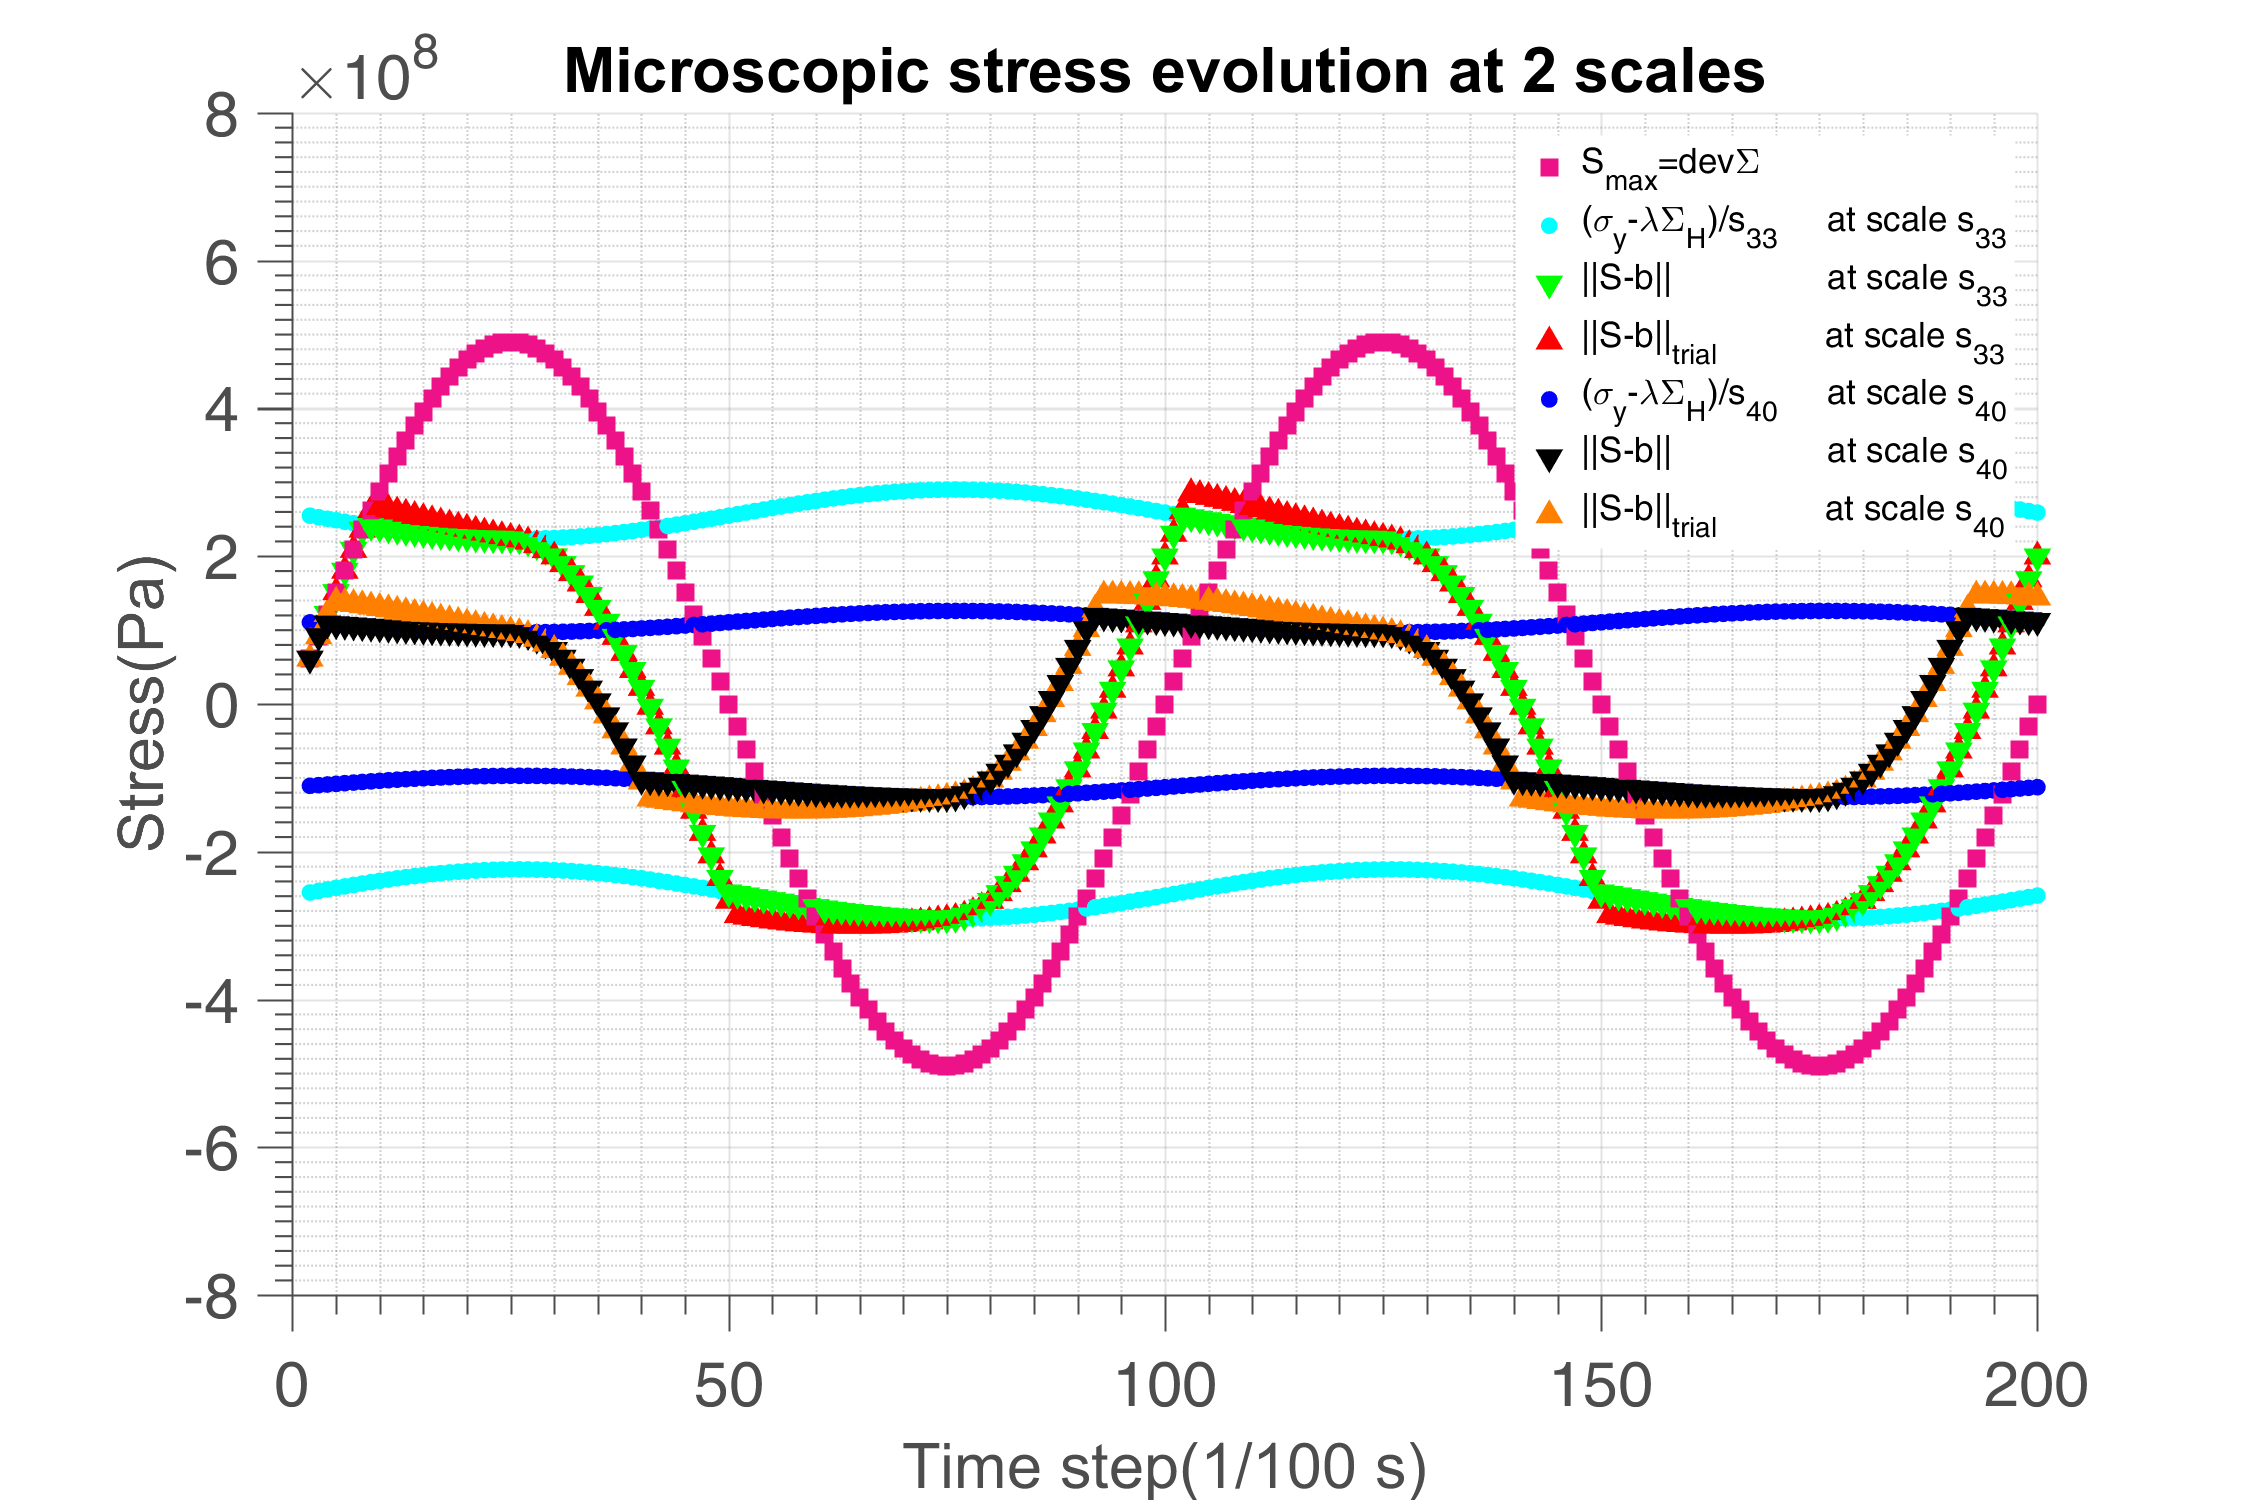
\includegraphics[width=\textwidth]{figures//trialsin_0.png} 
	\caption{Microscopic $\left(  \uline{\uline{S}}-\uline{\uline{b}}\right)_{trial}$ and $\left( \uline{\uline{S}}-\uline{\uline{b}}\right)$ evolution with time under different weakening scales($s_{33}=4.20$ and $s_{40}=9.68$) in sinusoidal load with zero mean stress}
	\label{fig.trialsin0}
\end{figure}
\begin{figure}[!h]
	\centering
	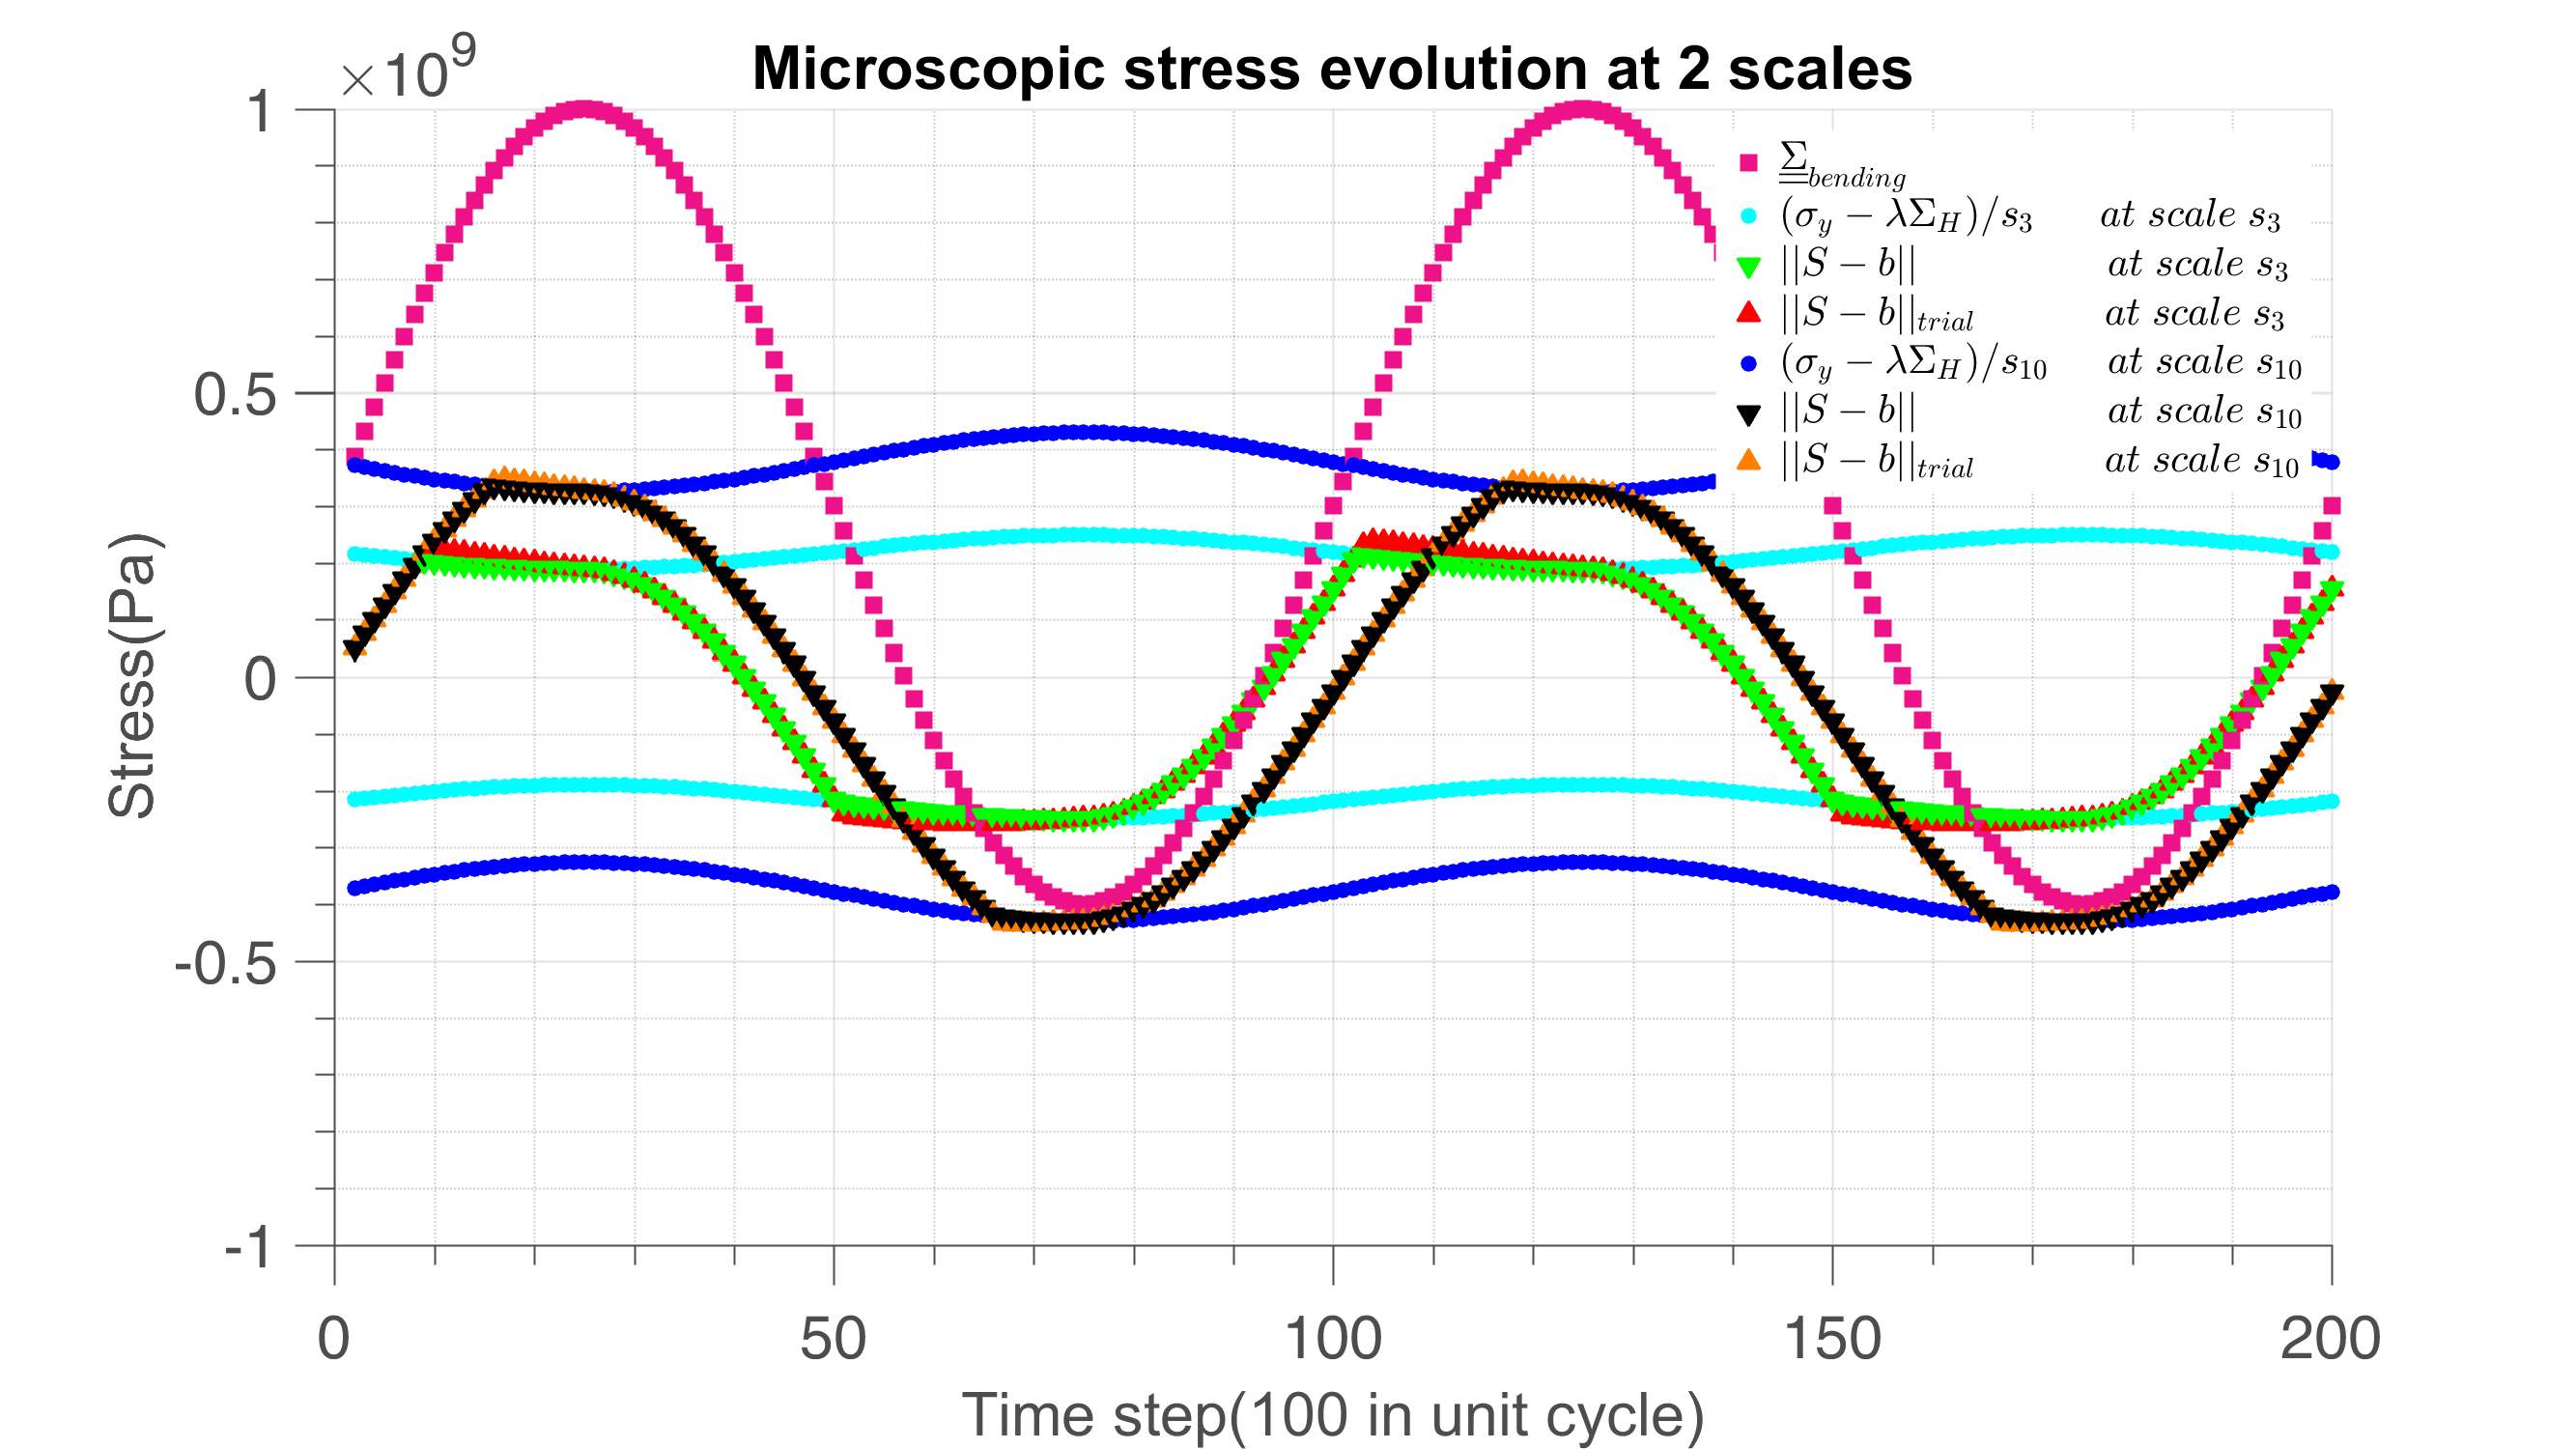
\includegraphics[width=\textwidth]{figures//trialsin_m.png} 
	\caption{Microscopic $\left(  \uline{\uline{S}}-\uline{\uline{b}}\right)_{trial}$ and $\left( \uline{\uline{S}}-\uline{\uline{b}}\right)$ evolution with time under different weakening scales($s_{33}=4.20$ and $s_{40}=9.68$) in sinusoidal load with non-zero mean stress}
	\label{fig.trialsinm}
\end{figure}

The dissipated energy per time step is depicted in \figref{fig.W3methods} with its enlargement in \figref{fig.W3methodsenlarge}. We scale $S_{max}$ in the plot to see more clear the relation between energy dissipation and stress intensity. The ``jump'' in energy evolution is due to activation of new scales while in-between two scales the dissipated energy follows the stress increment at each time step . $\alpha$ does not affect the dissipated energy $W$, only concerns damage accumulation rate.
\begin{figure}[!h]
	\centering
	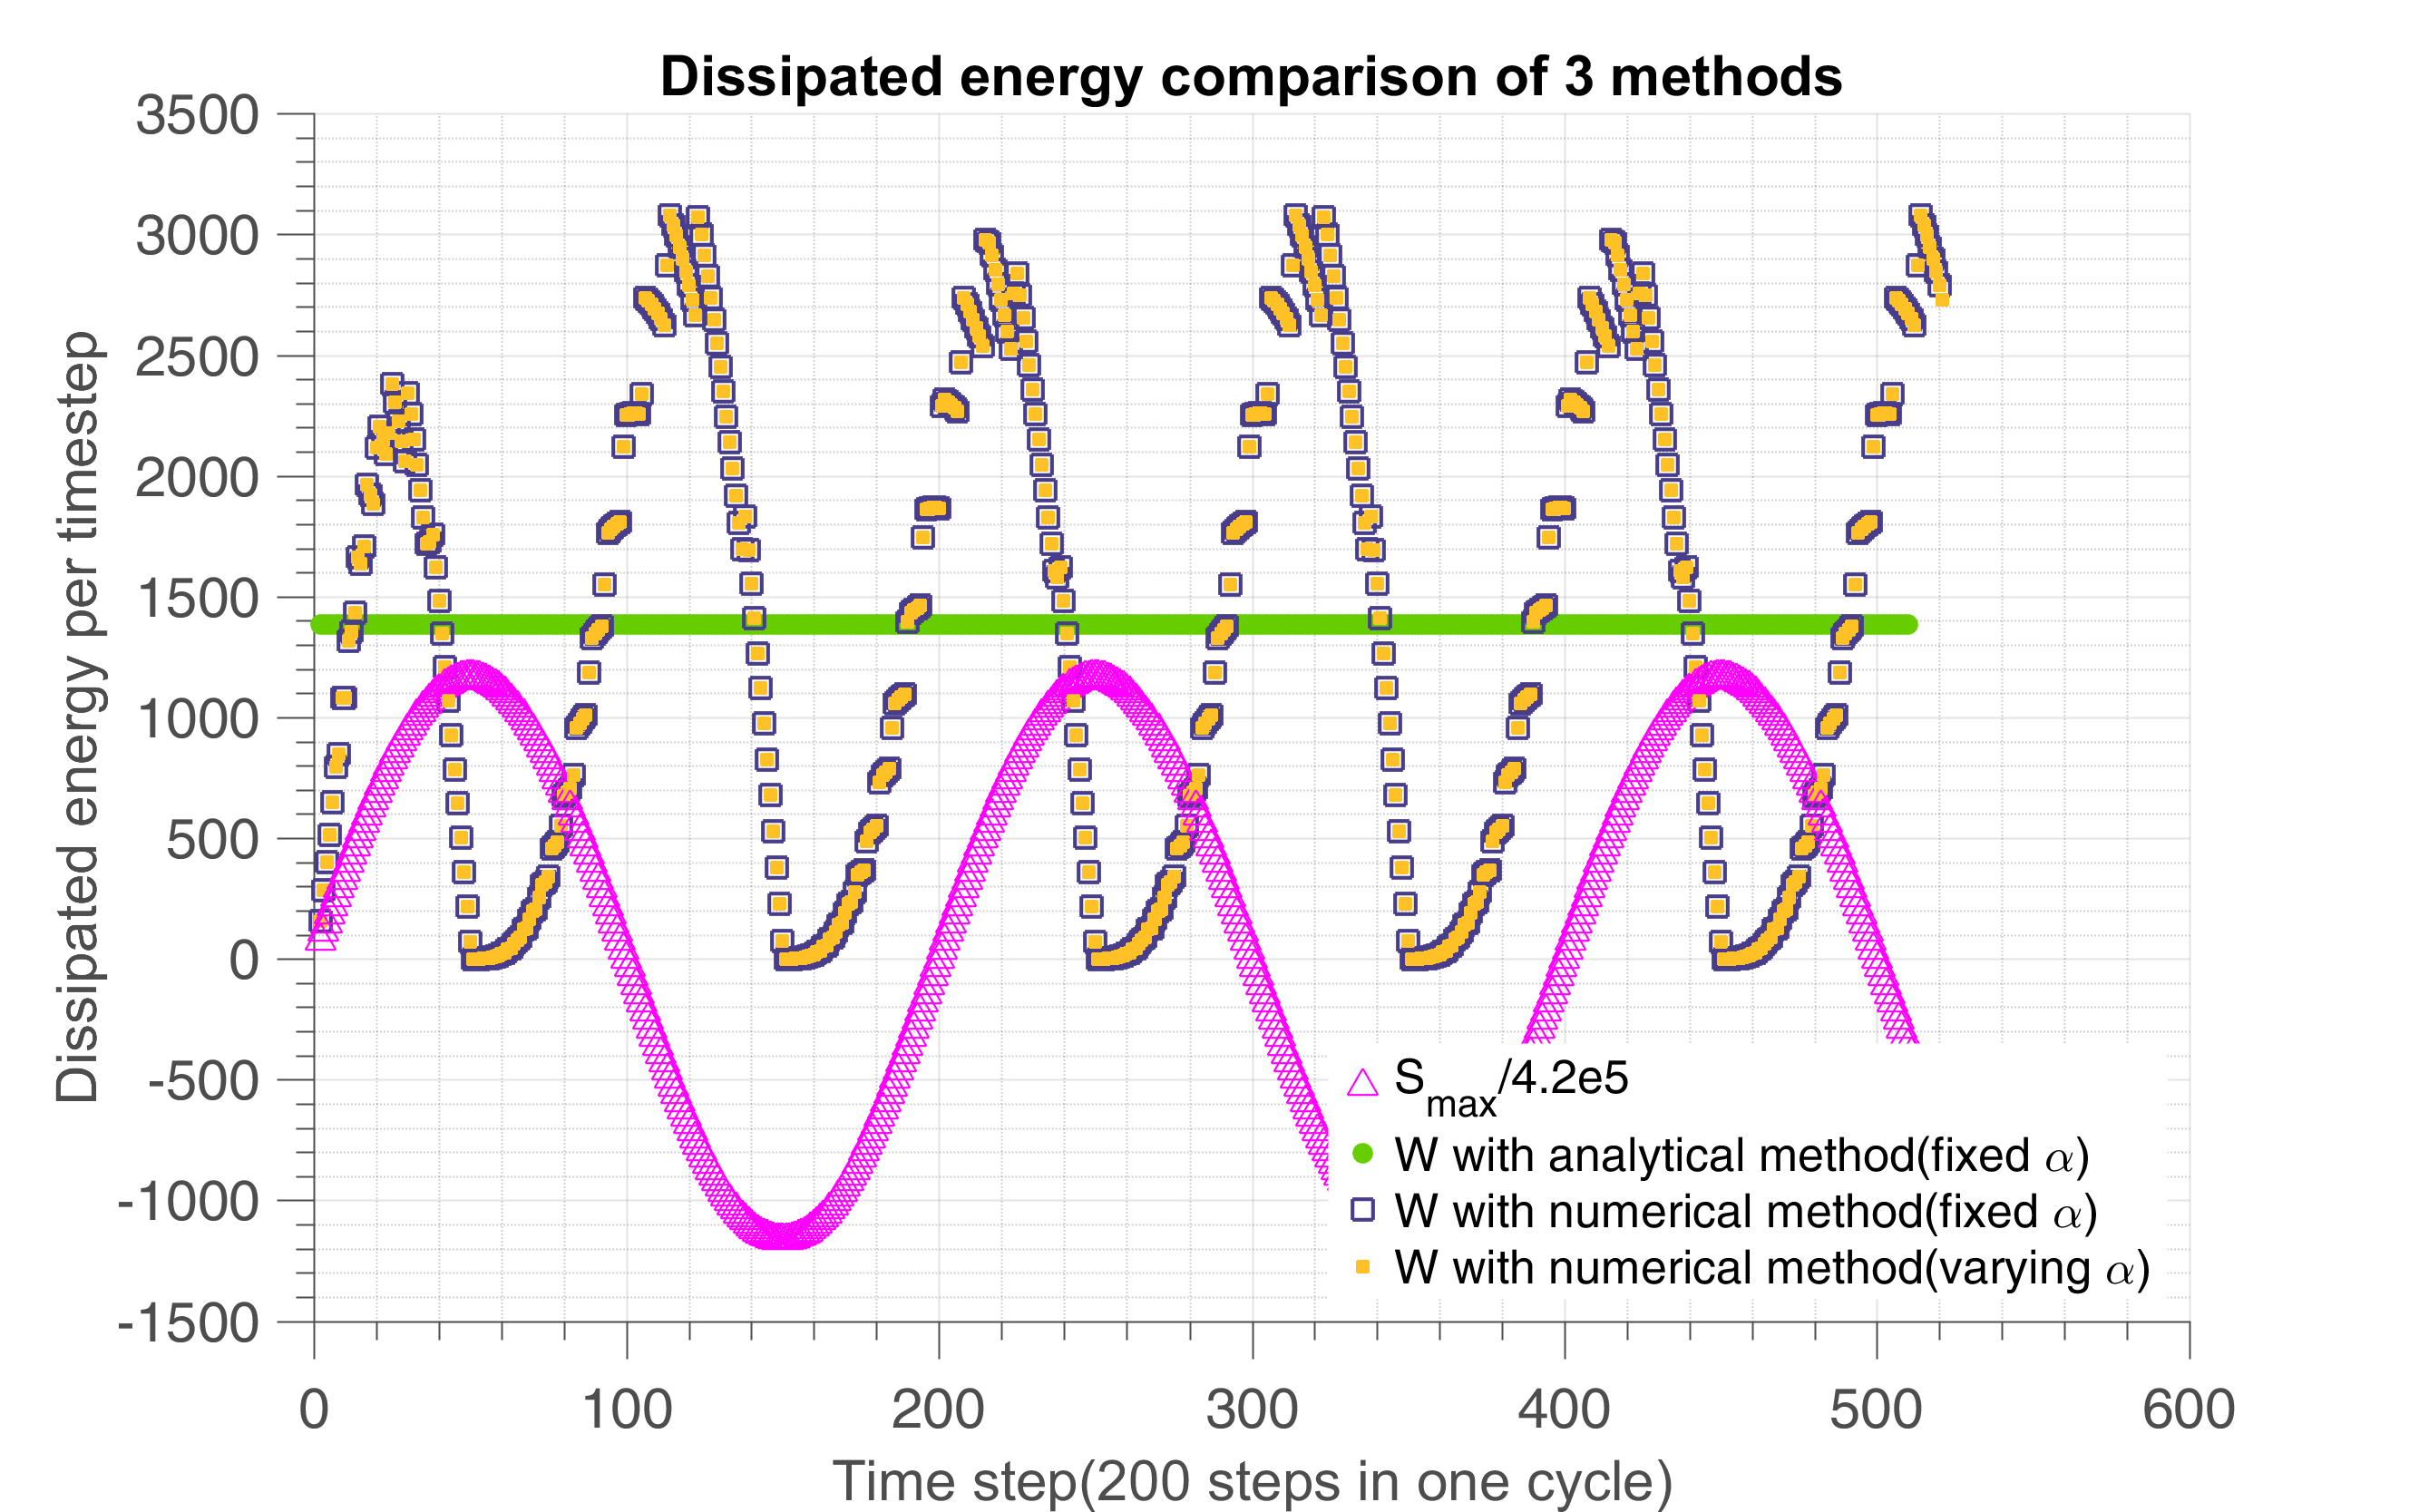
\includegraphics[width=0.95\textwidth]{figures//W_3methods.png} 
	\caption{Validation of dissipated energy in all scales with analytical and numerical method }
	\label{fig.W3methods}
\end{figure}

\begin{figure}[!h]
	\centering
	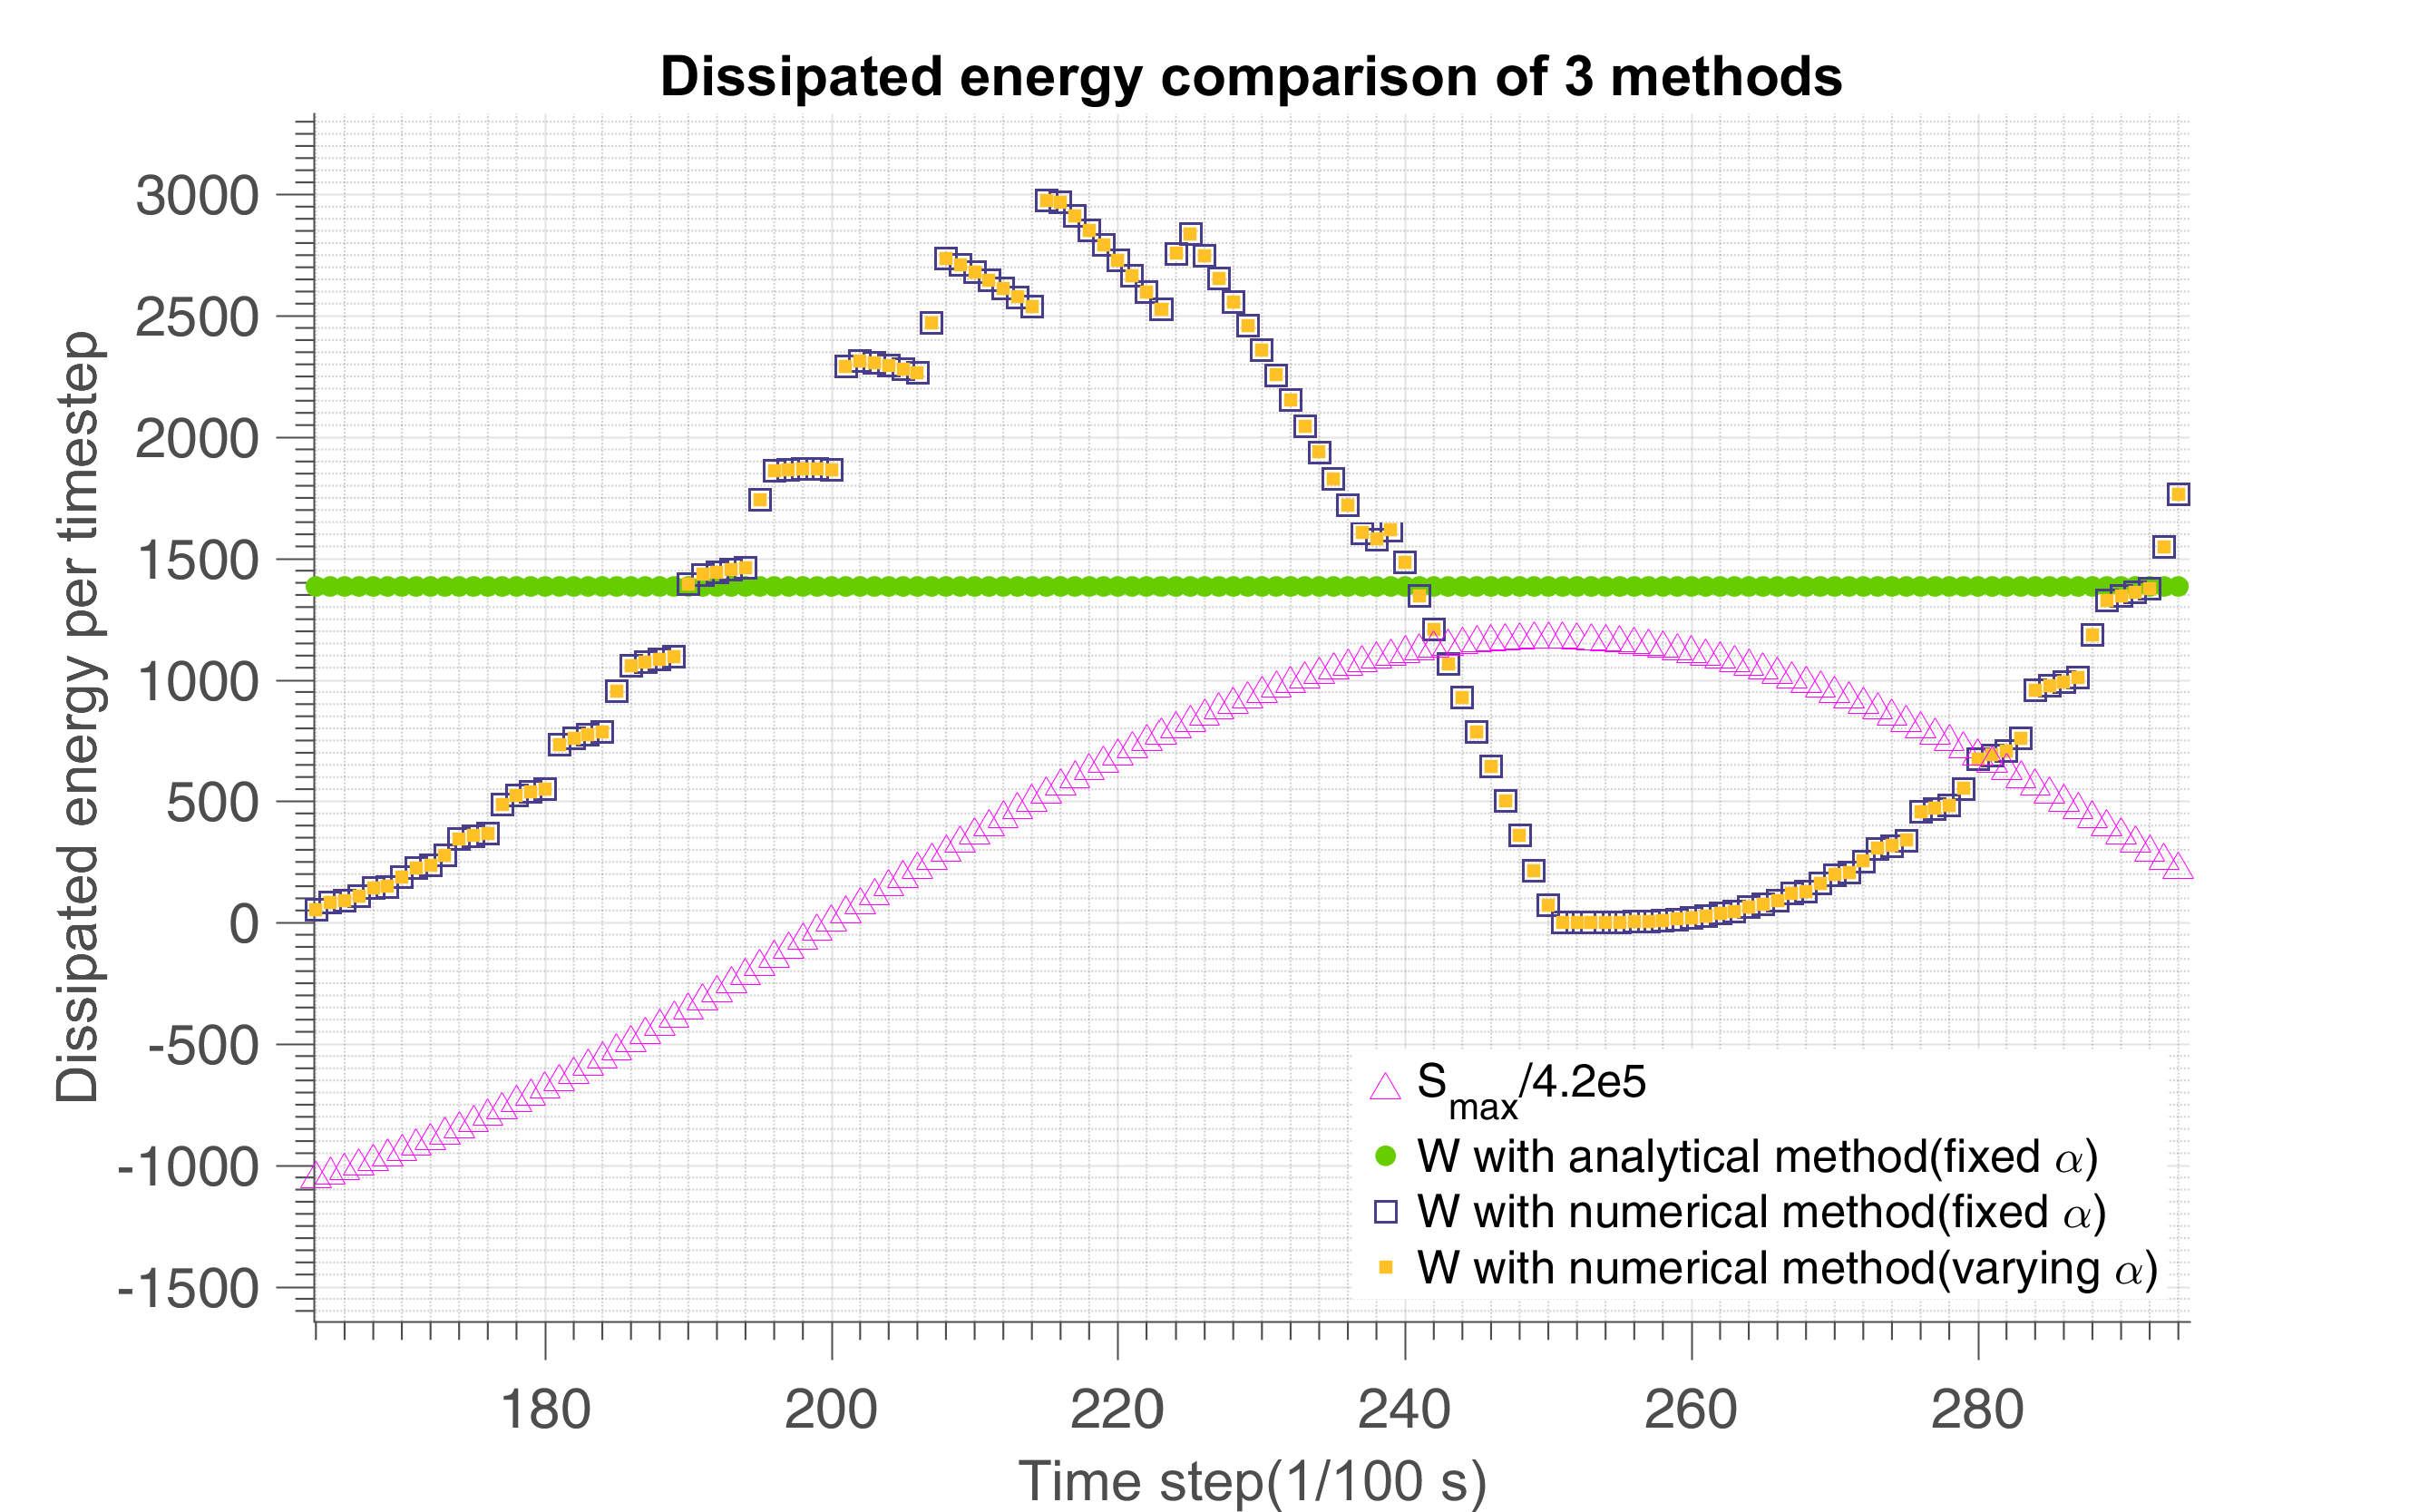
\includegraphics[width=0.95\textwidth]{figures//W_3methods_enlarge.png} 
	\caption{Partial enlargement of \figref{fig.W3methods}}
	\label{fig.W3methodsenlarge}
\end{figure}
The accumulated energy dissipation without damage accumulation law is shown in \figref{fig.W3methods2}. The difference between analytical energy loss and numerical one is shown in \figref{fig.W3methodsdiff}.
\begin{figure}[!h]
	\centering
	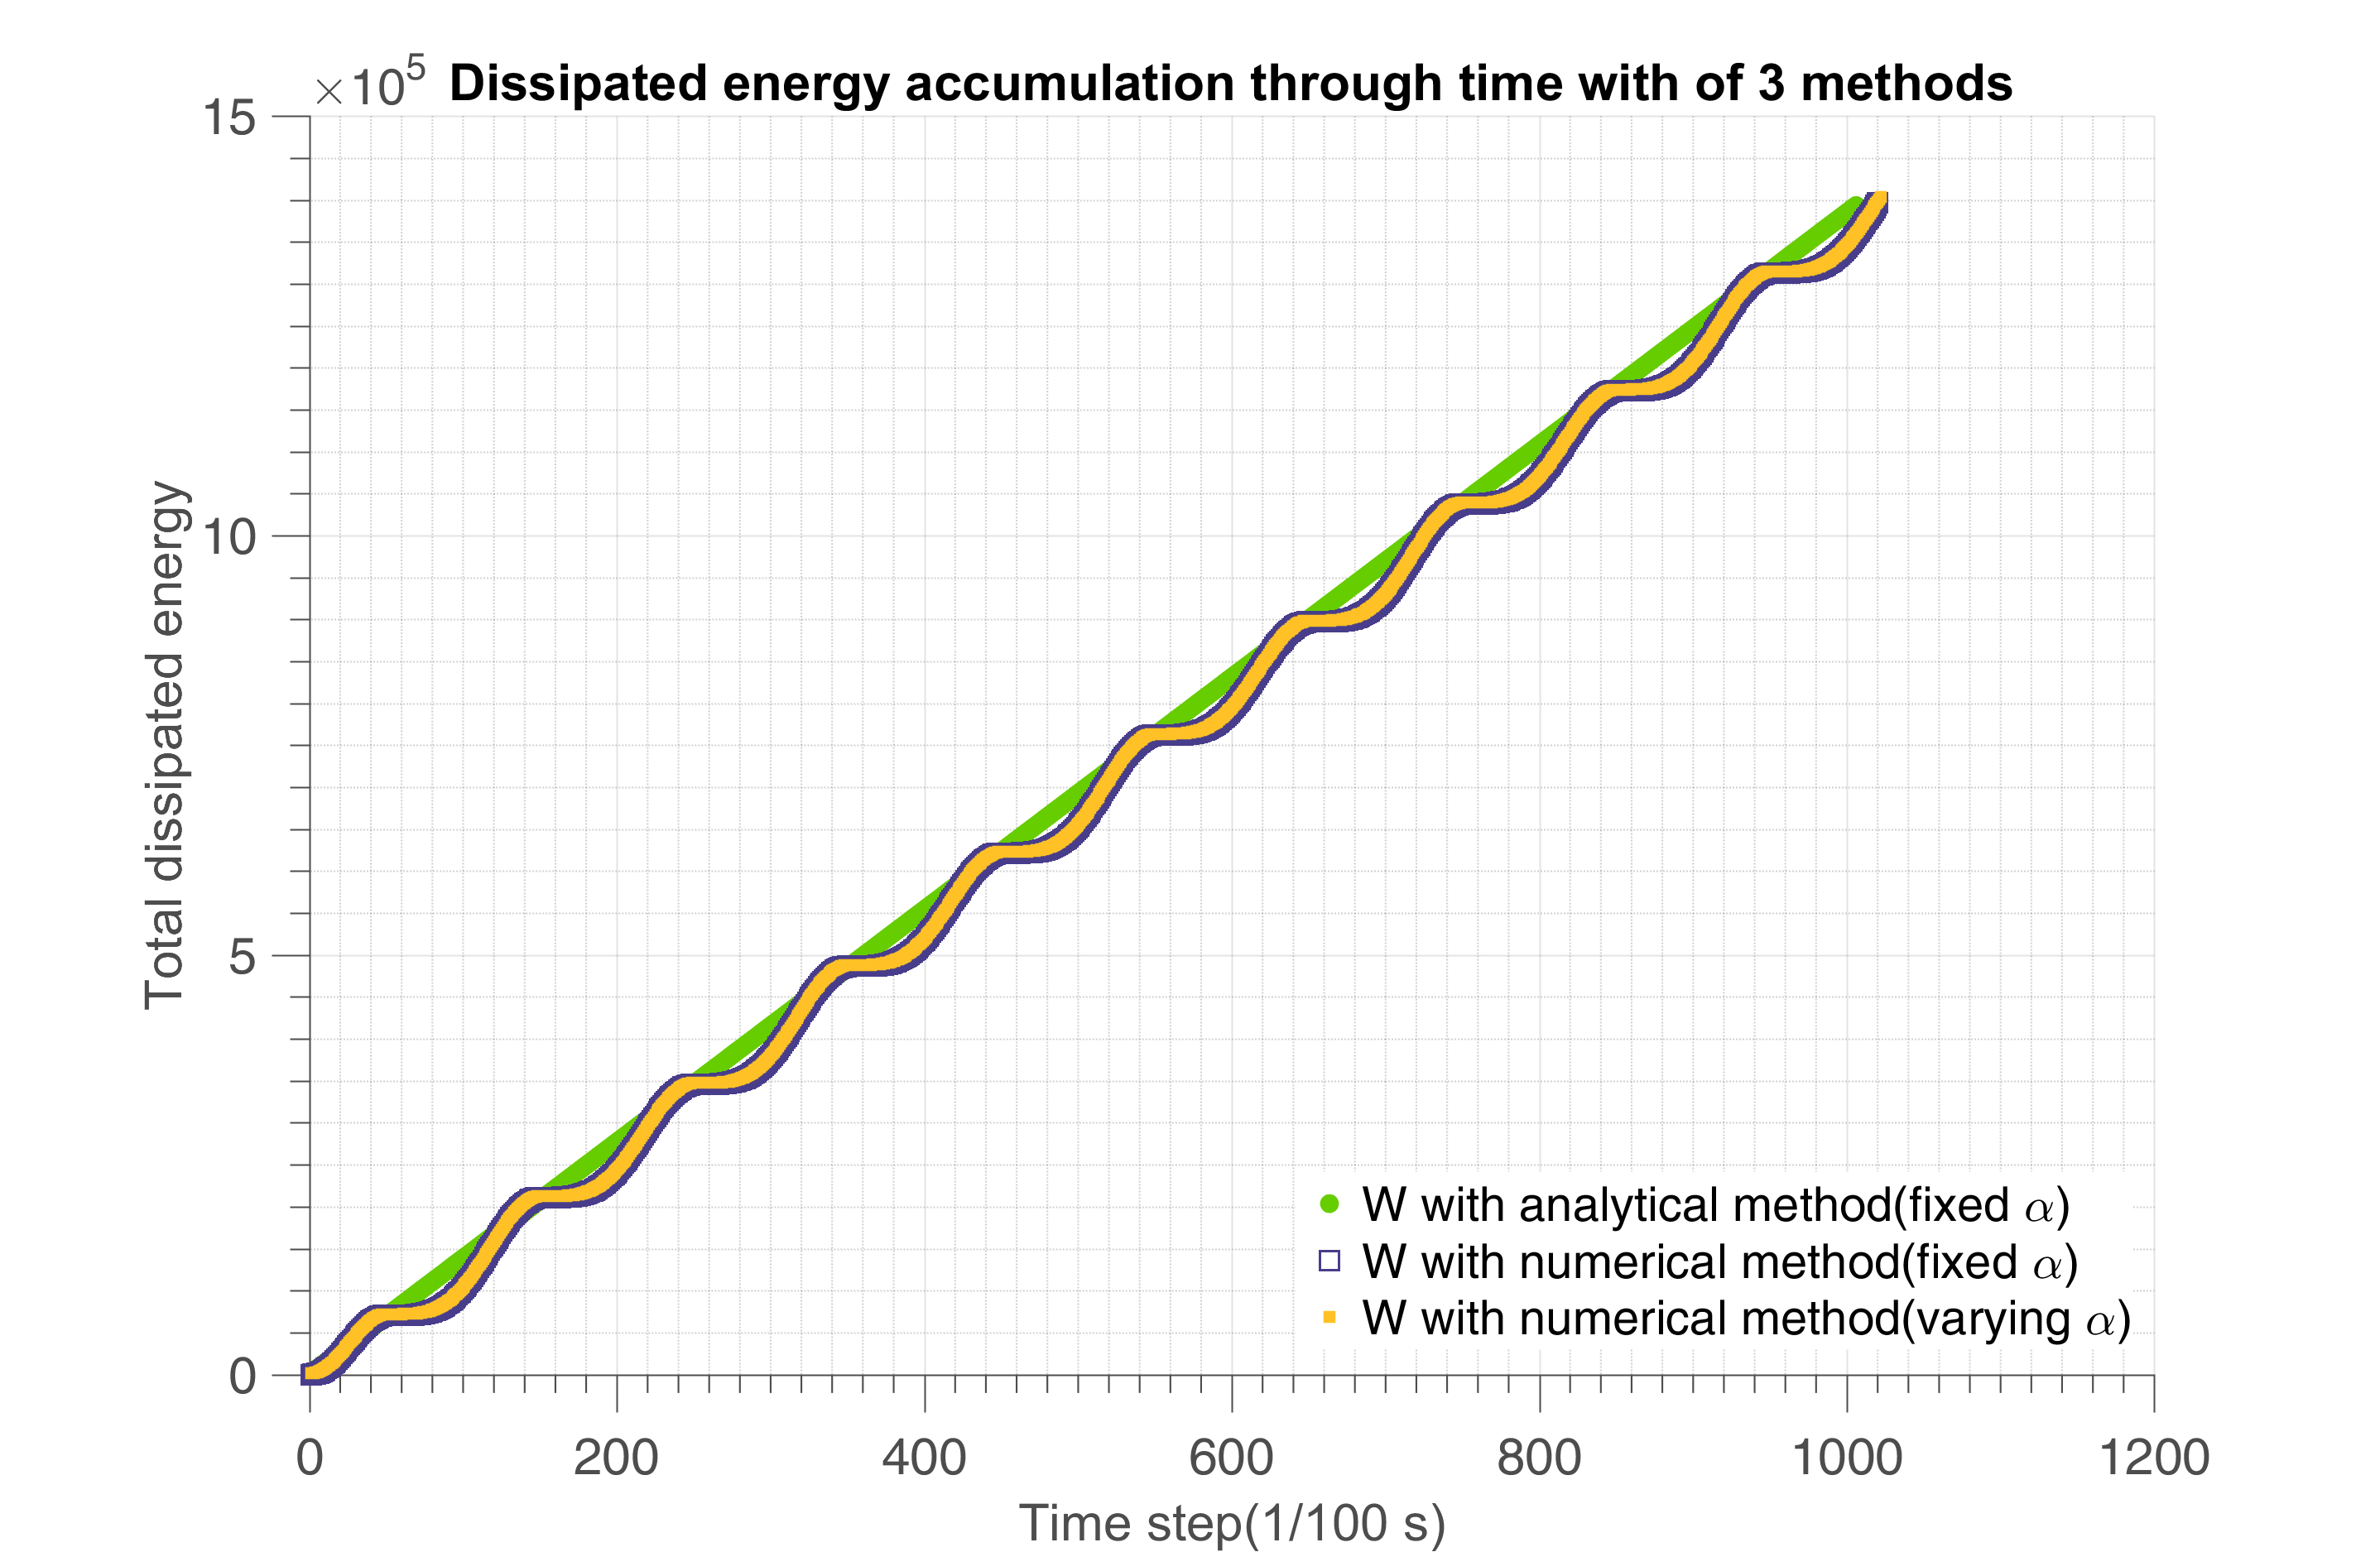
\includegraphics[width=0.95\textwidth]{figures//W_3methods2.png} 
	\caption{Dissipated energy accumulation through time with of 3 methods}
	\label{fig.W3methods2}
\end{figure}
\begin{figure}[!h]
	\centering
	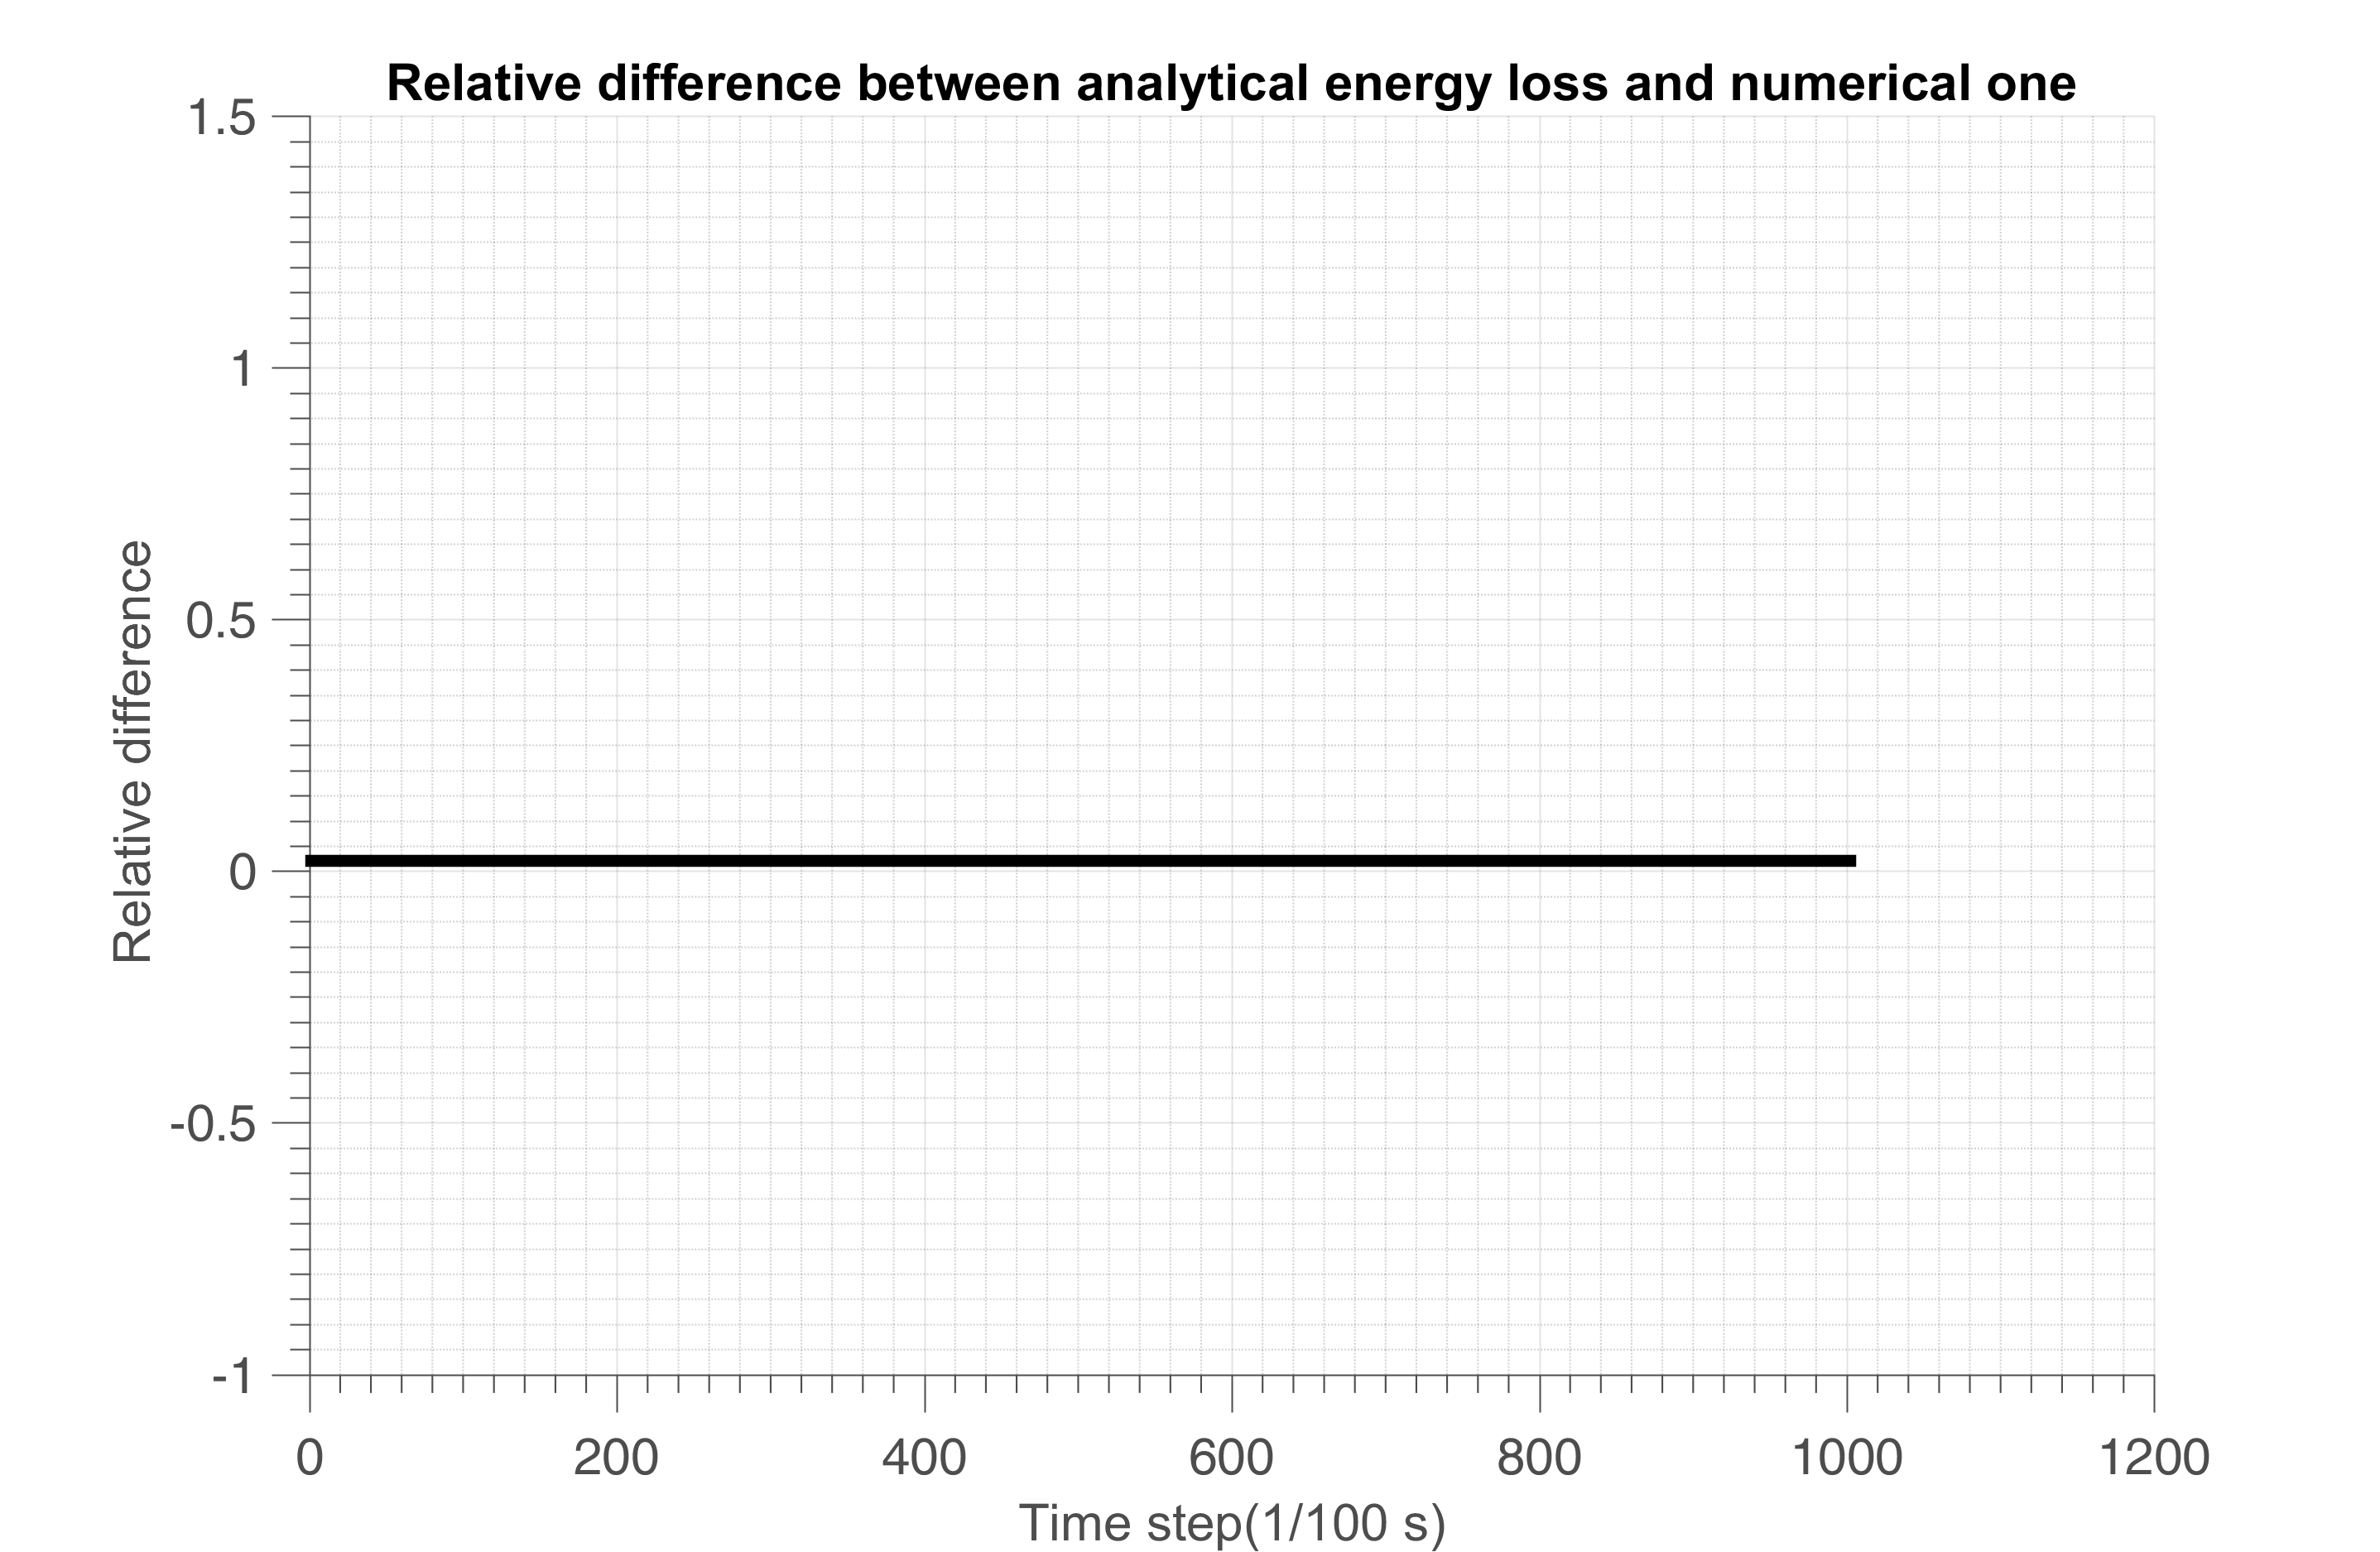
\includegraphics[width=0.95\textwidth]{figures//W_3methods_diff.png} 
	\caption{Relative difference $\dfrac{W_{analytical}-W_{numerical}}{W_{analytical}}$ between analytical energy loss and numerical one with $\alpha$ varying with time}
	\label{fig.W3methodsdiff}
\end{figure}
The damage evolves like in \figref{damsin}, where we compare the damage evolution as predicted by the cycle accumulation Eq.\eqref{eq:w} and by the numerical strategy of section 4.

\begin{figure}[!h]
	\centering
	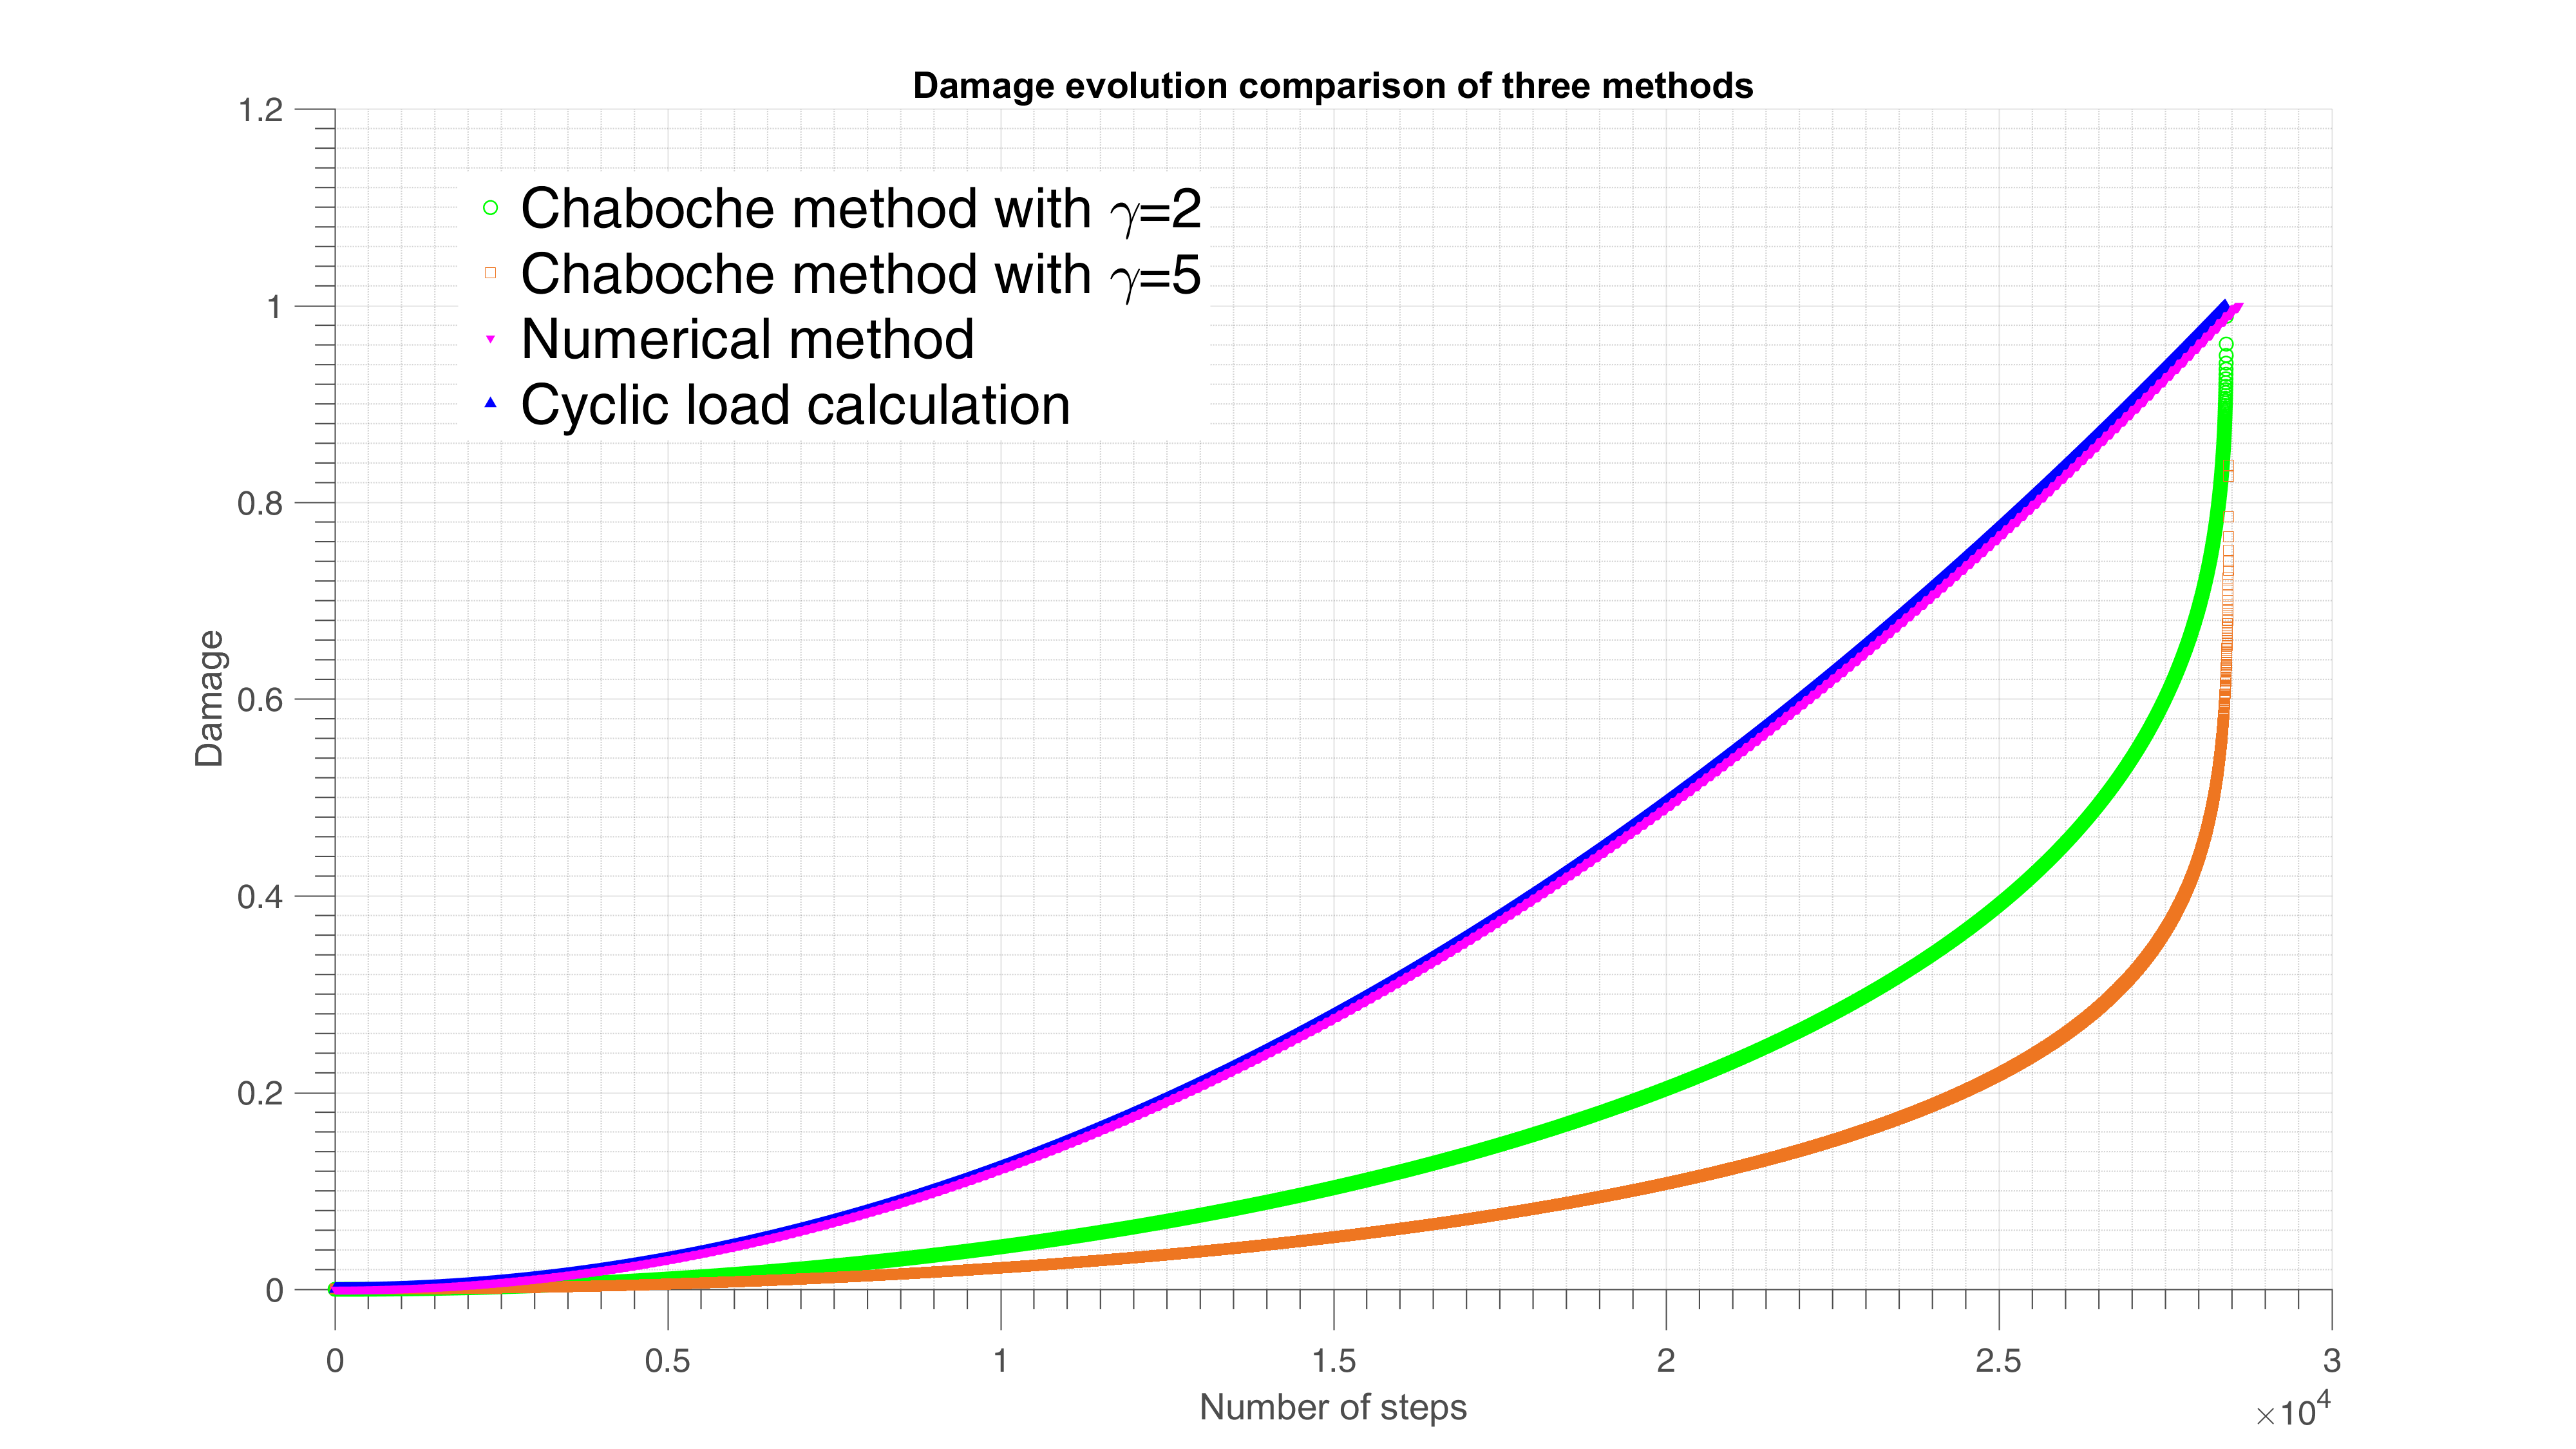
\includegraphics[width=\textwidth]{figures//damagesin.png} 
	\caption{Damage evolution with time under sinusoidal load with two different methods}
	\label{damsin}
\end{figure}

Now we compare the result to the one demonstrated in \figref{backstress}.  We can see from \figref{Damagediff}  the difference between cyclic load calculation and numerical method as function of time steps $n$. From the relative difference figure we conclude that the two methods converge.

\begin{figure}[!h]
	\centering
	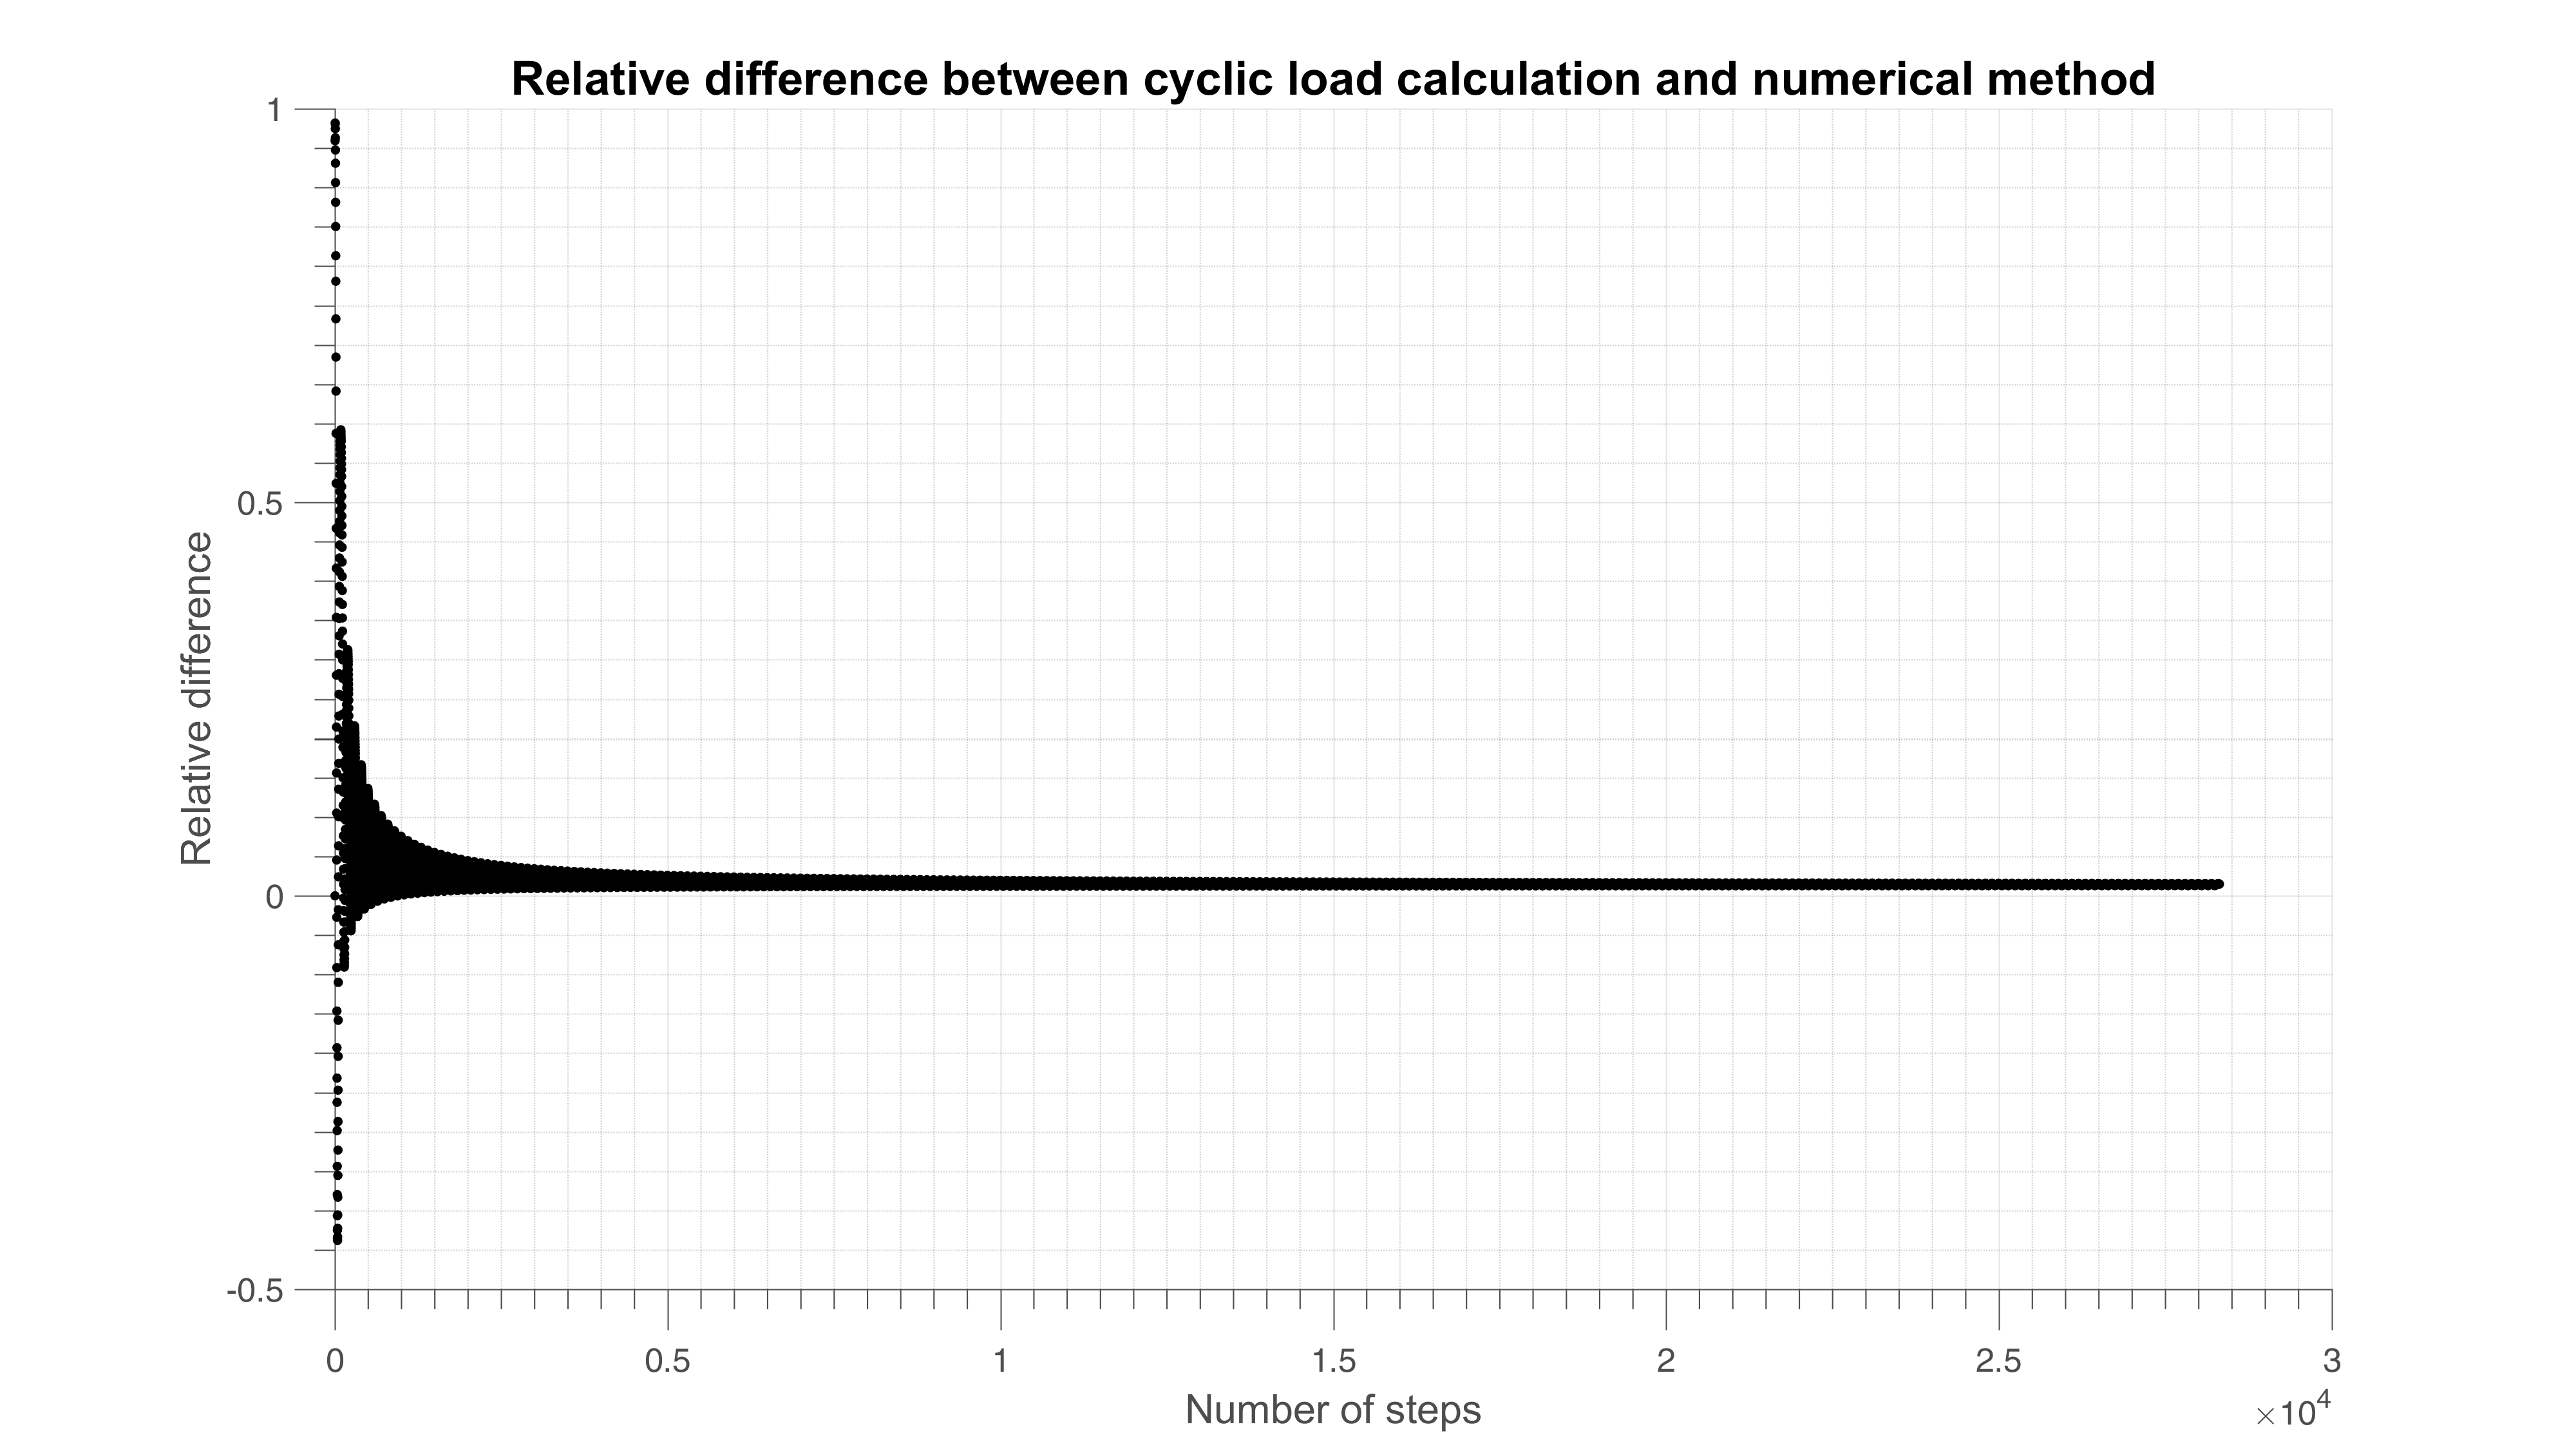
\includegraphics[width=\textwidth]{figures//Damagediff.png} 
	\caption{Relative difference $\dfrac{D_{analytical}-D_{numerical}}{D_{analytical}}$ evolution with time}
	\label{Damagediff}
\end{figure}

There is discrepancy between analytical damage and numerical damage calculation at the beginning, this is due to the numerical implementation difference that the analytical result is calculated by equally dividing the $W_{cyc}$ into 200 time steps in one cycle leading to constant dissipation per time step, whilst the numerical result is instantaneously calculated at each time step following stress evolution. So the numerical damage accumulation line swings around the analytical line. The relative difference is significant at the beginning but becomes negligible as number of steps gets larger.

The cyclic load calculation is only valid for very simple such as proportional loading in fatigue, nevertheless it can still be used as a comparison group to verify the numerical results. The outcome seems satisfactory. Hence, to be more general for any loading history, we adopt the numerical method.

\newpage
\subsection{Numerical recovery of sequence effect}
We adopt the parameter $\alpha$ to take into account the sequence effect. The high-low loading sequence clearly reduces the fatigue life, as depicted in \figref{sequence}. In order to cover this phenomenon, we let $\alpha$ change with time. Here $a$ is the sequence effect sensitivity, according to Eq.\eqref{eq.smin}, we have:
$$s_{min}(t)=\dfrac{\sigma_y-\lambda \Sigma_H(t)}{S_{max}(t)},$$
which is the minimum weakening scale that activates energy loss.  We use a general law for $\alpha$ of the type $\alpha = \alpha (s_{min})$ with the idea that for us $s_{min}$ is a measure of present intensity of macroscopic stress = mechanical based stress norm. 


Numerically we review our method of the sequence effect as depicted in \figref{sequence}.
\begin{Figure}[h!]{Two level sequence effect.}[sequence]
\graphfile*[30]{figures//high-low-Smax.png}[]
\graphfile*[30]{figures//low-high-Smax.png}[]
\\
\graphfile*[30]{figures//high-low-alp.png}[]
\graphfile*[30]{figures//low-high-alp.png}[]
\\
\graphfile*[30]{figures//high-low-D.png}[]
\graphfile*[30]{figures//low-high-D.png}[]
\label{sequence}
\end{Figure}


\clearpage
\section{Experimental verification}
\subsection{Constant amplitude 1D tests from Cetim on AW-6106 T6 aluminum}

The tests are performed on aluminum batches, the characteristics of the sample are shown in table.\ref{tab:cetim}.
\begin{figure}[!h]
	\centering
	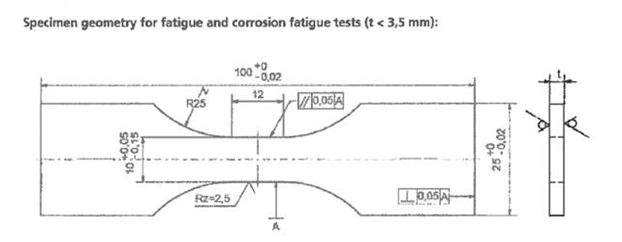
\includegraphics[width=0.7\textwidth]{figures//aluminum_cetim.png} 
	\caption{Specimen geometry for fatigue tests of AW-6106 T6 aluminum}
	\label{fig:aluminum}
\end{figure}
\begin{table}[!h]
	\centering
	\begin{tabular}{ll}
		\hline
		\textbf{Parameters}                                         & \textbf{Value}                    \\ \hline
		Young's modulus                                             & $E=72$ GPa                       \\
		Hardening parameter                                         &  $k=8.5$ MPa \\
		Macroscopic yield stress                                    & $\sigma_y=230$ MPa              \\
		Thickness & $e=2.9mm$                        \\
		Width		 & $l= 9.95mm$                        \\ \hline
	\end{tabular}
	\caption{Material parameters}
	\label{tab:cetim}
\end{table}

\textbf{Comparison of fixed and varying $\alpha$ with constant amplitude loading}

The parameters we introduced during the deduction need to be calibrated. The source of the parameter identification are listed in Table.\ref{paras}.
In the case of constant amplitude loading, analytically $\alpha$ does not change with time because $S_{max}$ is a linear function of stress intensity. However, numerically $\alpha$ changes with time because real life experiments have fluctuations. The comparison with the average $\alpha$ are shown in \figref{fig:alpha}. The relative error of number of points to failure $n_F$ is 0.142\%.

\begin{figure}[!h]
	\centering
	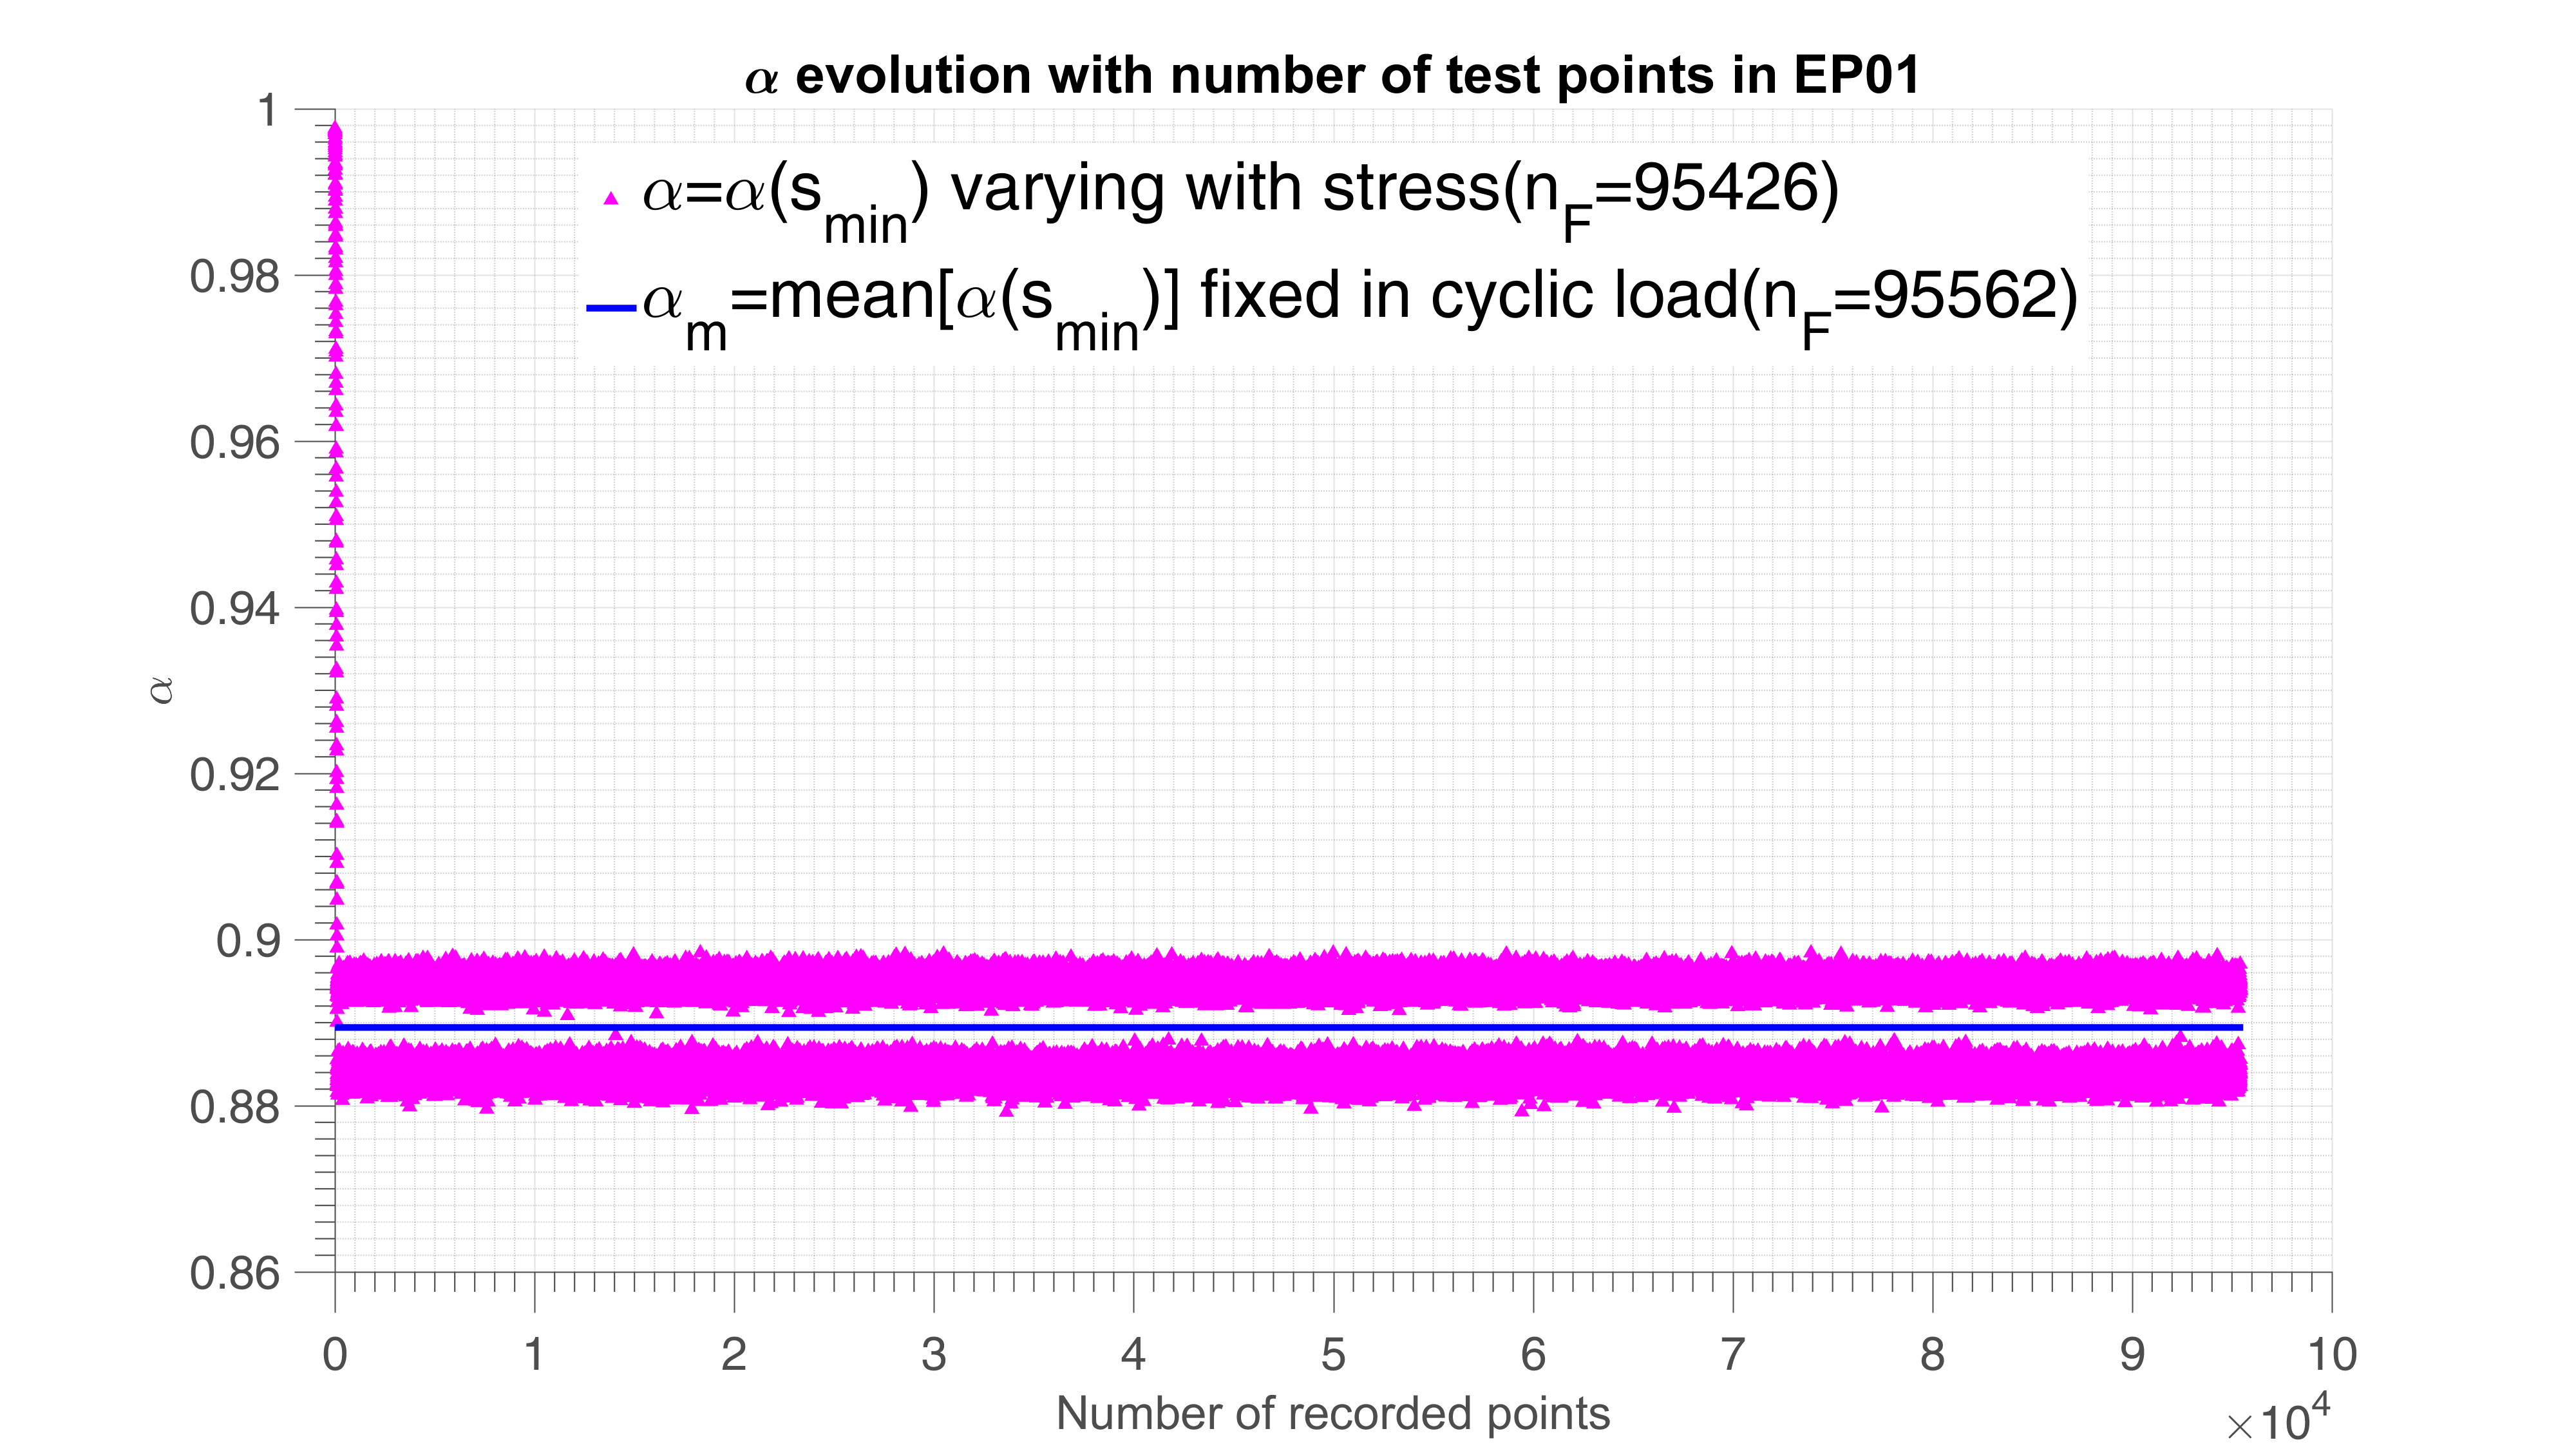
\includegraphics[width=\textwidth]{figures//alpha_fix_vs_change.png} 
	\caption{Different choice of alpha numerically}
	\label{fig:alpha}
\end{figure}

For instance in constant amplitude loading, the number of cycles to failure according to Eq.\eqref{eq.NFWcyc} with fixed $\alpha$ is expressed as Eq.\eqref{eq.nf}:
\begin{equation}
\begin{split}
N_F&=\dfrac{W_0}{\left( 1-\alpha\right)W_{cyc} }
\\&= \frac{W_0}{\left( 1-\alpha\right) }\dfrac{E(E+k\nu)\beta\left( \beta+1\right) }{ 4(E-k)(1+\nu)\left( \beta-1\right) }\dfrac{\left(\sigma_y-\lambda \Sigma_H\right)^{\beta-1}}{S_{max}^{\beta+1} }  .
\end{split}
\label{eq.nf}
\end{equation}


We now apply this formulation to a simple cyclic load with mean stress $m$ applied on aluminum having $\Sigma_y=230MPa$.
$$\Sigma(n)=Asin(\pi/2+n\pi)+m.$$
Which gives $\Sigma_{max}=A+m$ and $\Sigma_{min}=-A+m$. We give $m=0.1A$. $S_{max}=\sqrt{\frac{2}{3}}A$ in cyclic loading is the amplitude of deviatoric stress and independent from mean stress $m$.

Where n is the number of recorded points. Similar as shown in \figref{fig:alpha} with negligible error, in $S-N$ curve there is only cyclic loading with constant amplitude, so we analytically use the mean value of $\alpha$ for the damage accumulation part and $\left(\sigma_y-\lambda \Sigma_H\right)_m$ for the energy dissipation part through one cycle to give $N_F$ at each point in $S-N$ curve. However, $\alpha_m$ is not fixed with constant amplitude of loading case, it depends on the loading pattern. Normal stresses act to pull parallel planes within the material apart or push them closer
together, while shear stresses act to slide planes along one another. Normal stresses promote
crack formation and growth, while shear stresses underlie yield and plastic slip. 

Published data on the yield strength of steels and
other structural materials is typically limited to values
determined from uniaxial tension tests. The yield strength is
customarily defined as that value of tensile stress which when
relaxed to zero results in an unrecovered strain of 0.2\%. The
torsional yield strength ( $\tau_y$) is generally assumed to be 0.5–0.6
of this tensile value, based on one or another of the several
popular theories of plasticity\cite{dieter1961mechanical}.
 Here we give two methods to get $\alpha_m$ as shown in \figref{fig.alpmean}.

\begin{figure}[!h]
	\centering
	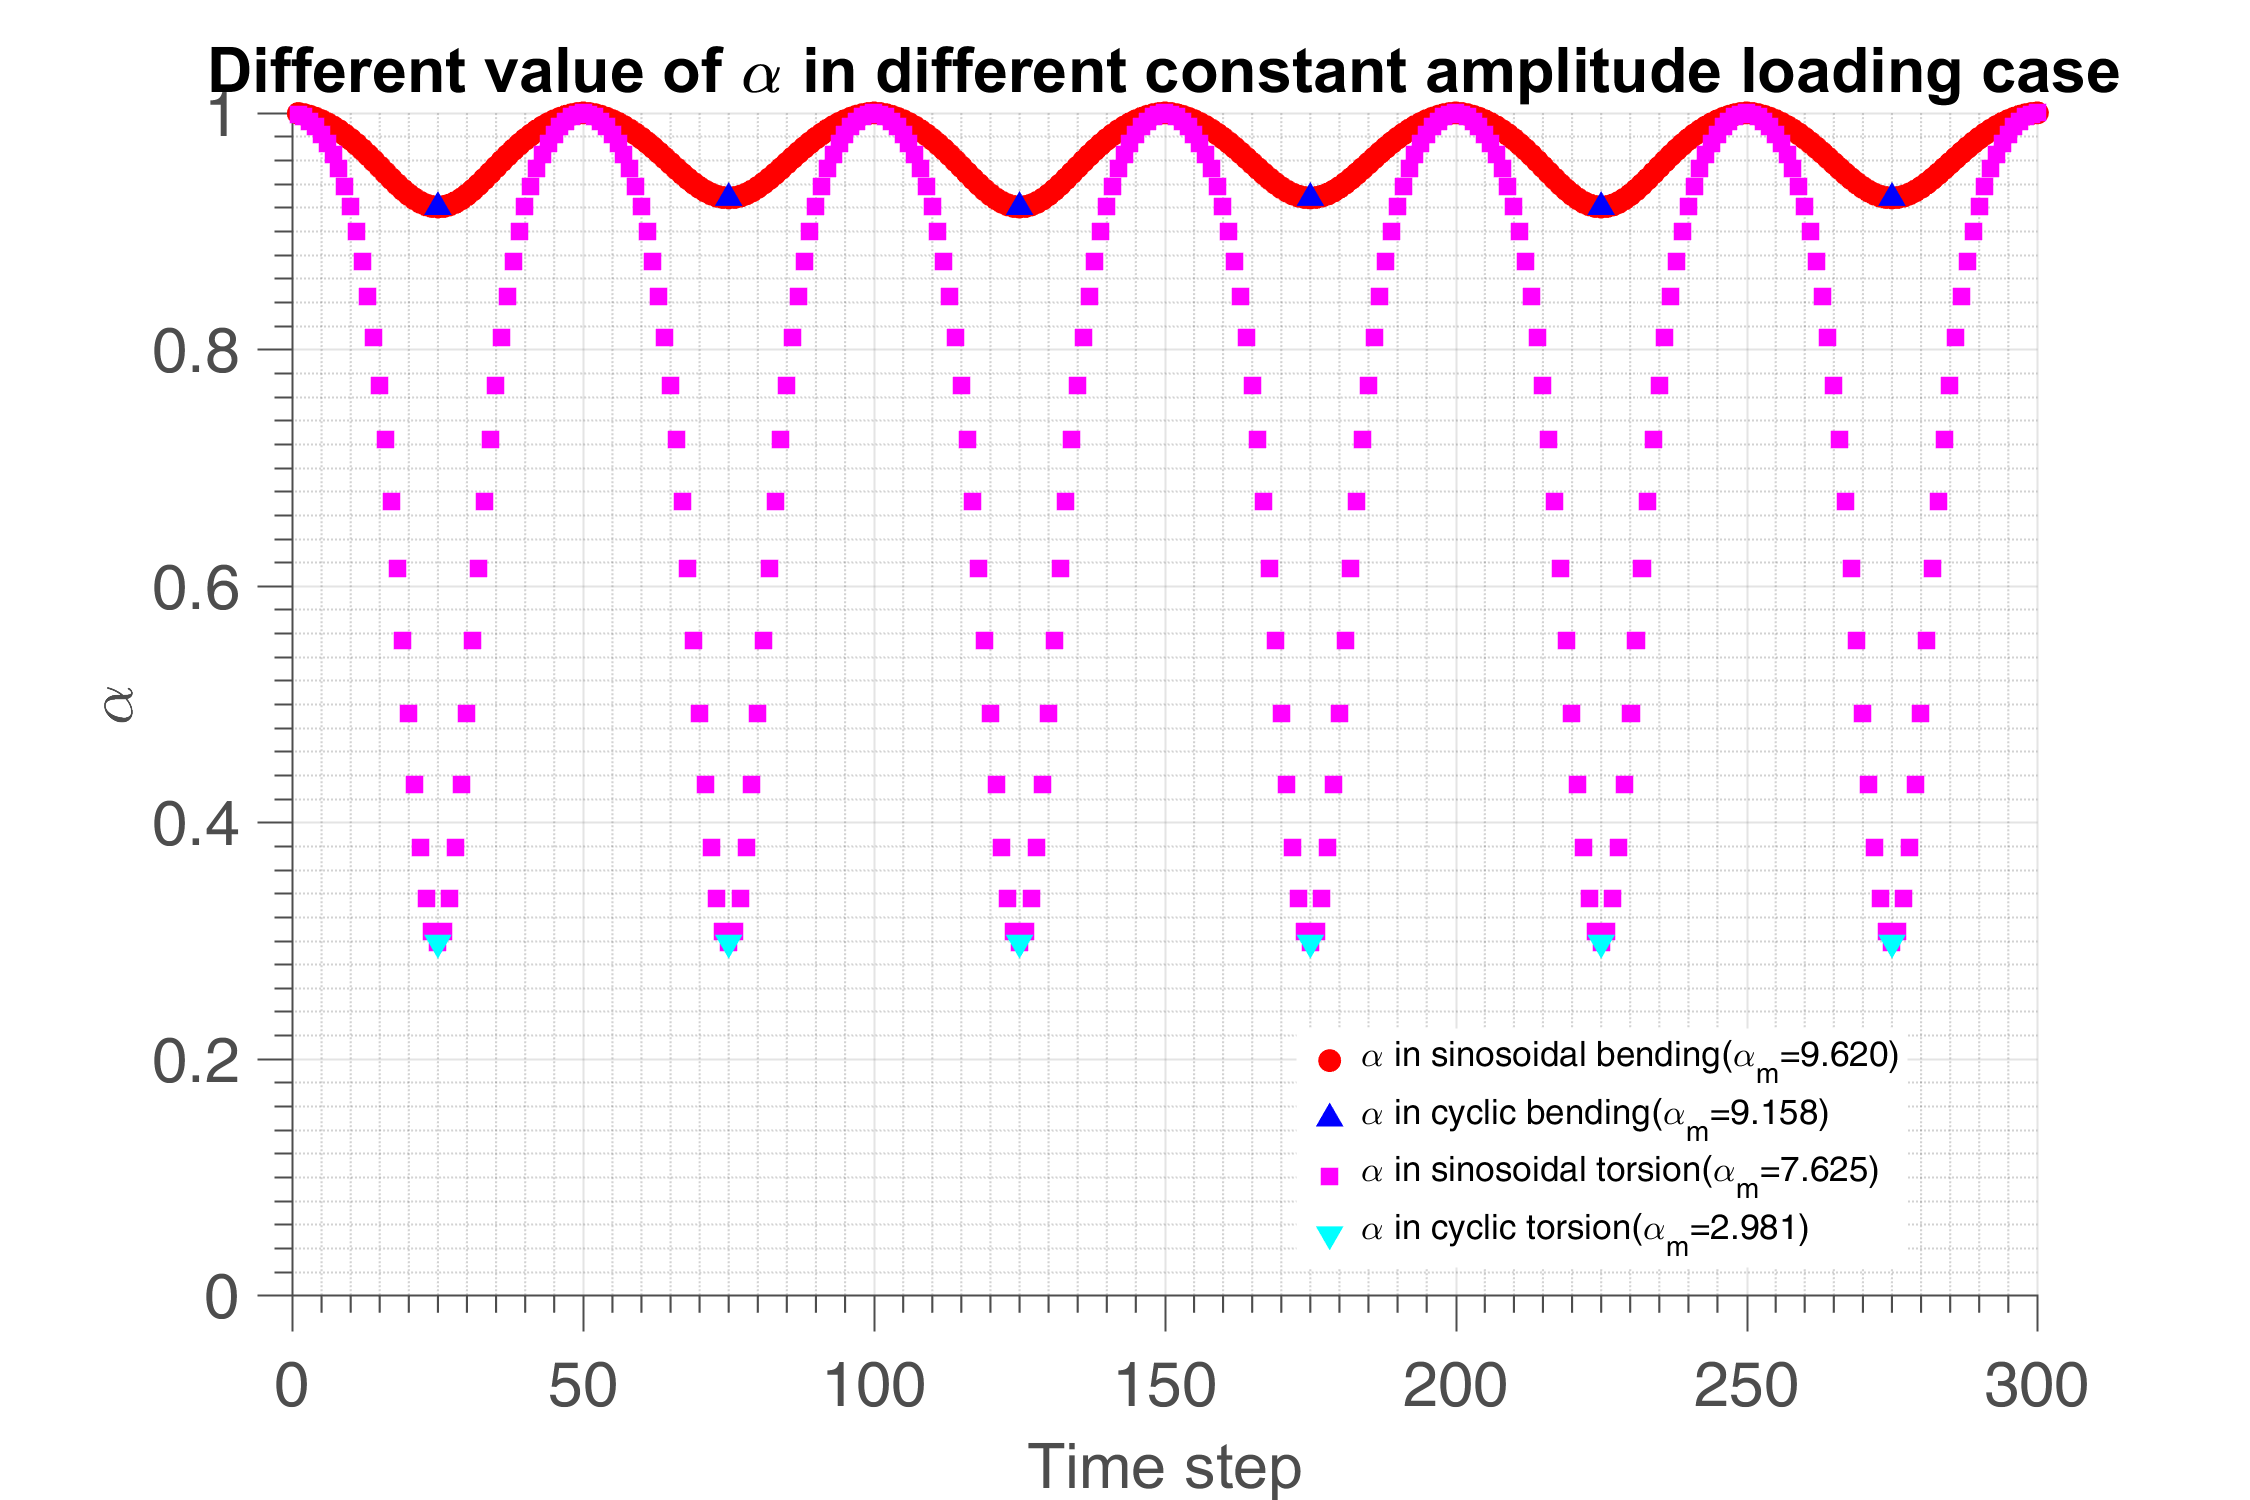
\includegraphics[width=0.8\textwidth]{figures//alp_mean_methods.png} 
	\caption{Comparing different calculation methods of $\alpha_m$}
	\label{fig.alpmean}
\end{figure}



We have in damage accumulation part as in Eq.\eqref{eq.alpm}:
\begin{equation}
\alpha_m=\dfrac{\alpha(s_{min1})+\alpha(s_{min2})}{2}=\dfrac{\left[ 1-a\left(  s_{min1}-1 \right) ^{-\beta}\right] +\left[ 1-a\left(  s_{min2}-1 \right) ^{-\beta}\right] }{2},
\label{eq.alpm}
\end{equation}
with
$$s_{min1}=\dfrac{\left(\sigma_y-\lambda \dfrac{\Sigma_{max}}{3}\right)}{S_{max}},$$
$$s_{min2}=\dfrac{\left(\sigma_y-\lambda \dfrac{\Sigma_{min}}{3}\right)}{S_{max}}.$$


The mean parameter we give concerning the energy dissipation part is:
$$\left(\sigma_y-\lambda \Sigma_H\right)_m=\dfrac{\left(\sigma_y-\lambda\dfrac{\Sigma_{max}}{3}\right)+\left(\sigma_y-\lambda \dfrac{\Sigma_{min}}{3}\right)}{2}=\sigma_y-\lambda \dfrac{m}{3}.$$
This deduction give the mean value of dissipated energy in one cycle in constant amplitude loading as in Eq.\eqref{eq.wcycm}:
\begin{equation}
W_{cycm}=\dfrac{4(E-k)(1+\nu)\left( \beta-1\right) }{ E(E+k\nu)\beta\left( \beta+1\right) }\dfrac{S_{max}^{\beta+1} }{\left(\sigma_y-\lambda \dfrac{m}{3}\right)^{\beta-1}}.
\label{eq.wcycm}
\end{equation}

The final expression to validate cyclic loading experiments is expressed as in Eq.\eqref{eq.nfm}.
\begin{equation}
N_F=\dfrac{W_0}{\left( 1-\alpha_m\right)W_{cycm} }.
\label{eq.nfm}
\end{equation}
Once $\alpha_m$ is fixed in constant amplitude cyclic loading, this parameter has the same influence as $W_0$. The parameters remain to calibrate are $\lambda$ on the mean stress sensitivity and distinction between bending and torsion, $\beta$ on the slope of $S-N$ curve.

What should we use for $S_{max}$ in the presence of mean stress? The amplitude or the mean value of \{max,min\}?
I used the later method in the fitting of 30NCD16, SM45C and 10HNAP steel:
The stress tensor $\uuline{\sigma}$ is then:
\begin{equation} 
\uline{\uline{\sigma}}(t)=
\left(
\begin{array}{ccc}
\sigma_{a}sin(\omega t)+m & \tau_asin(\omega t) & 0\\
\tau_asin(\omega t) & 0 & 0\\ 
0 & 0 & 0\\
\end{array}\right) .
\end{equation}

with deviator
\begin{equation} 
\uuline{S}=\uuline{\sigma}-\dfrac{1}{3}\textrm{tr}\uuline{\sigma}=
\left(
\begin{array}{ccc}
\dfrac{2}{3}\left( \sigma_{a}sin(\omega t)+m\right)  & \tau_asin(\omega t) & 0\\
\tau_asin(\omega t) & -\dfrac{1}{3}\left( \sigma_{a}sin(\omega t)+m\right)& 0\\ 
0 & 0 & -\dfrac{1}{3}\left( \sigma_{a}sin(\omega t)+m\right)\\
\end{array}\right) .
\end{equation}

Here I use:
$$S_{max}=mean(\sqrt{\uuline{S}^2}).$$

The method of take the mean values of $\alpha$, $\sigma_y$ and $S_{max}$ analytically in the presence of mean stress or in the case of multiaxial loading is not feasible here. We propose in constant amplitude load it is necessary to numerically calculate the mean values of $\alpha$ and $W_{cycm}$ through several cycles and apply the result via  Eq.\eqref{eq.nfm}. The assumption is for constant amplitude loading the energy dissipation is time independent as shown in \figref{fig.W3methods2}. In this way the numerical cost is neither as high as step by step numerical implementation in random amplitude loading case, nor inaccurate as analytical mean value method. 

\newpage
\subsection{Random amplitude 1D tests from Cetim on AW-6106 T6 aluminum}

There are 12 validated uniaxial fatigue tests on the AW-6106 T6 aluminum sample, in which 2 are constant amplitude load case and 10 random  load case. 
The cyclic stress of test number 1(ep01) and test number 2(ep02) are respectively $131.9MPa$ and $97.0MPa$. We first identify the same parameters feasible to both loading cases. 

\begin{figure}[!h]
	\centering
	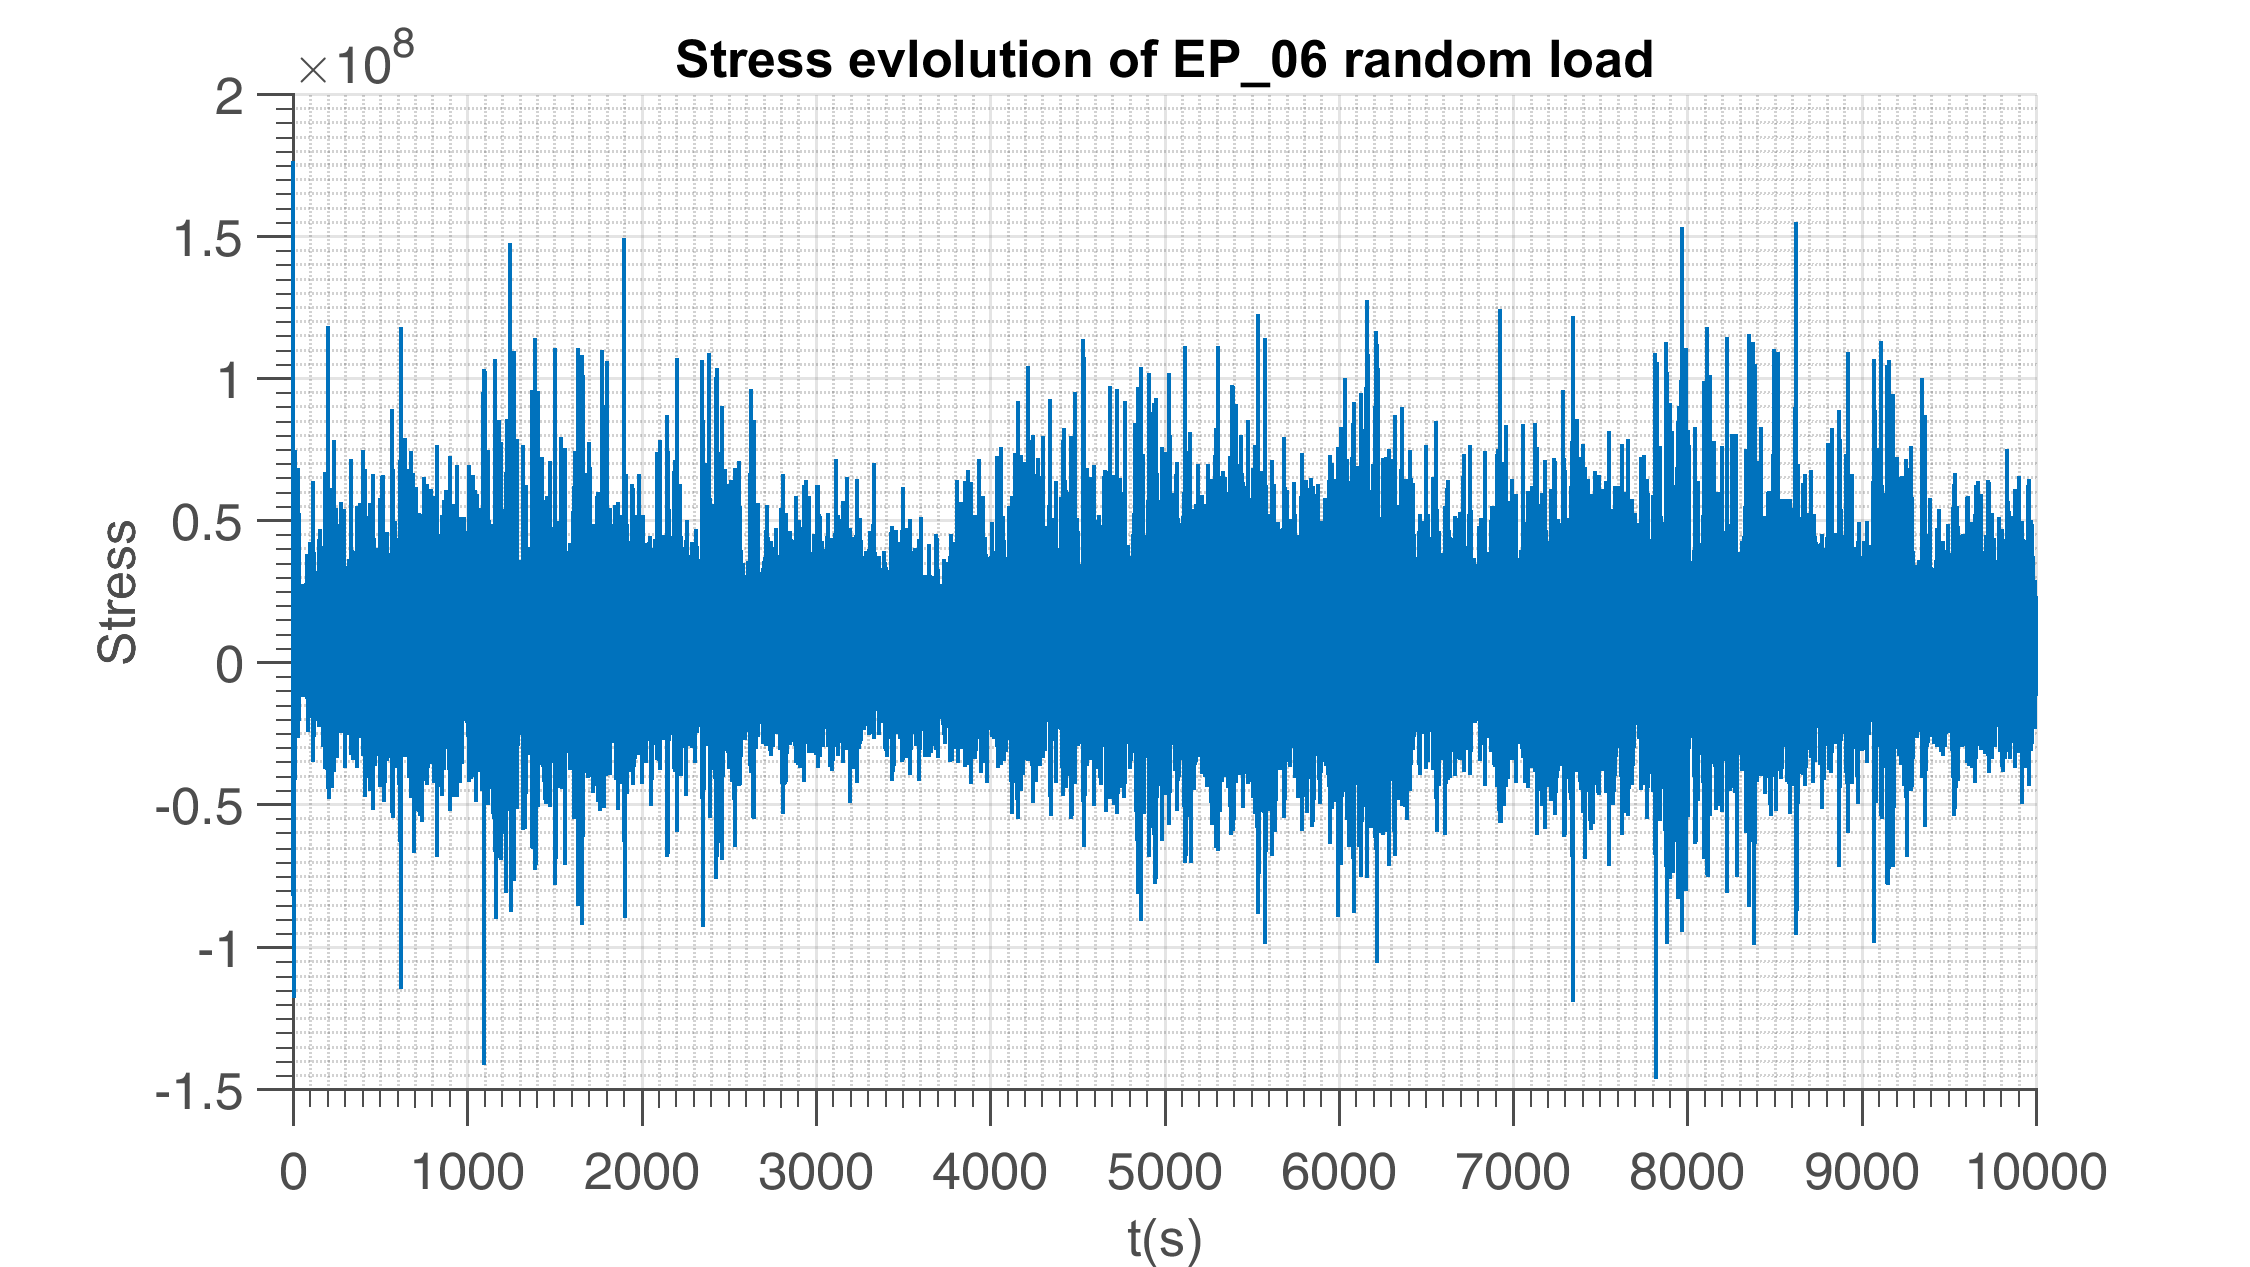
\includegraphics[width=\textwidth]{figures//ep_06_stress.png} 
	\caption{Random loading history on batch 06 of AW-6106 T6 aluminum}
\end{figure}	
The detailed tests information are shown in table.\ref{tab:Cetim}. There are 27000($\pm 2.4\%$) recorded points per repetition. 

\begin{table}[!h]
	\centering
	\begin{tabular}{lllll}
		\hline
		\textbf{Specimen} & \textbf{Fmax (kN)} & \textbf{$\Sigma_{max}$ in the block} & \textbf{Number of repetition} & \textbf{Number of points} \\ \hline
		BATCH\_A\_01      & 3.375              &                                      &                                          & 99892                                \\
		BATCH\_A\_02      & 2.475              &                                      &                                          & 414298                               \\
		BATCH\_A\_04      & nom                & 225.88                               & 95                                       & 2500000                              \\
		BATCH\_A\_05      & nom                & 225.88                               & 156                                      & 4105263                              \\
		BATCH\_A\_06      & nom                & 225.88                               & 145                                      & 3815789                              \\
		BATCH\_A\_07      & nom                & 225.88                               & 90                                       & 2368421                              \\
		BATCH\_A\_08      & nom                & 225.88                               & 194                                      & 5105263                              \\
		BATCH\_A\_09      & nom                & 225.88                               & 197                                      & 5184211                              \\
		BATCH\_A\_10      & nom x 0,9          & 203.292                              & 515                                      & 13552632                             \\
		BATCH\_A\_11      & nom x 0,9          & 203.292                              & 385                                      & 10131579                             \\
		BATCH\_A\_12      & nom x 0,9          & 203.292                              & 424                                      & 11157895                             \\
		BATCH\_A\_13      & nom x 0,9          & 203.292                              & 409                                      & 10763158                             \\ \hline
		BATCH\_B\_01      & nom                & 225.88                               & 121                                      & 3184211                              \\
		BATCH\_B\_02      & nom x 0,8          & 180.704                              & 380                                      & 10000000                             \\
		BATCH\_B\_03      & nom x 0,8          & 180.704                              & 380                                      & 10000000                             \\
		BATCH\_B\_04      & nom x 0,9          & 203.292                              & 406                                      & 10684211                             \\
		BATCH\_B\_05      & nom x 0,9          & 203.292                              & 454                                      & 11947368                             \\
		BATCH\_B\_06      & nom x 0,9          & 203.292                              & 518                                      & 13631579                             \\
		BATCH\_B\_07      & nom x 0,9          & 203.292                              & 553                                      & 14552632                             \\
		BATCH\_B\_08      & nom x 0,9          & 203.292                              & 612                                      & 16105263                             \\
		BATCH\_B\_09      & nom                & 225.88                               & 253                                      & 6657895                              \\
		BATCH\_B\_10      & nom                & 225.88                               & 196                                      & 5157895                              \\
		BATCH\_B\_11      & nom                & 225.88                               & 178                                      & 4684211                              \\
		BATCH\_B\_12      & nom                & 225.88                               & 123                                      & 3236842                              \\ \hline
	\end{tabular}
	\caption{Cetim fatigue tests result on AW-6106 T6 aluminum}
	\label{tab:Cetim}
\end{table}

We assume the material parameters like Young's modulus, hardening parameter, hydrostatic pressure sensitivity, macroscopic yield stress, Wohler curve exponent and sequence effect parameters are known. We first identify the weakening scales distribution, and dissipated energy to failure from cyclic tests ep01 and ep02. Then change the parameter $n_0$ to see if our assumption is correct or need to be changed. 



The numerical fitting process show that the damage is caused mainly by large stresses. The definition of major stress now need to be specified according to the material. To take into account this effect we first find out the proportion stress above a certain value in the repetition signal of random loading, as shown in Table.\ref{tab.majordamage}.  Here ep\_a and ep\_b are the same material. Since the samples were extracted from aluminum profiles of industrial production,  the two batches only  correspond to two different times of sampling in the production. The variation is supposed to be representative of the regular tolerances you might have in the production. ep\_a\_01 and ep\_a\_02 are constant amplitude loading which helps identify the power of weakening scale distribution $\beta$. ep\_a\_03 is low cycle fatigue data.  ep\_b\_02 and ep\_b\_03 have infinite life time. The data in the table are grabbed from random signal high cycle fatigue loading history.

\begin{table}[!h]
	\centering
	\begin{tabular}{llllllll}
		\hline
		\textbf{Stress\textgreater}  & \textbf{70}    & \textbf{90}    & \textbf{110}   & \textbf{130}    & \textbf{150}    & \textbf{170}    & \textbf{190}    \\
		\textbf{$S_{max}$\textgreater} & \textbf{57.15} & \textbf{73.48} & \textbf{89.81} & \textbf{106.14} & \textbf{122.47} & \textbf{138.80} & \textbf{155.13} \\
		\textbf{$X$}                 & \textbf{0.497} & \textbf{0.639} & \textbf{0.781} & \textbf{0.923}  & \textbf{1.065}  & \textbf{1.207}  & \textbf{1.349}  \\ \hline
		\textbf{ep\_a\_04}           &                & 1.962\%        & 0.904\%        & 0.077\%         & 0.037\%         & 0.018\%         & 0.007\%         \\
		\textbf{ep\_a\_05}           &                & 1.604\%        & 0.784\%        & 0.044\%         & 0.030\%         & 0.007\%         & 0.007\%         \\
		\textbf{ep\_a\_06}           &                & 1.645\%        & 0.784\%        & 0.045\%         & 0.030\%         & 0.007\%         & 0.007\%         \\
		\textbf{ep\_a\_07}           &                & 1.632\%        & 0.788\%        & 0.048\%         & 0.029\%         & 0.007\%         & 0.007\%         \\
		\textbf{ep\_a\_08}           &                & 1.644\%        & 0.787\%        & 0.048\%         & 0.037\%         & 0.007\%         & 0.007\%         \\
		\textbf{ep\_a\_09}           &                & 1.655\%        & 0.800\%        & 0.048\%         & 0.037\%         & 0.007\%         & 0.007\%         \\
		\textbf{ep\_a\_10}           &                & 0.768\%        & 0.134\%        & 0.007\%         & 0.000\%         & 0.000\%         & 0.000\%         \\
		\textbf{ep\_a\_11}           &                & 0.772\%        & 0.145\%        & 0.007\%         & 0.000\%         & 0.000\%         & 0.000\%         \\
		\textbf{ep\_a\_12}           &                & 0.779\%        & 0.133\%        & 0.011\%         & 0.000\%         & 0.000\%         & 0.000\%         \\
		\textbf{ep\_a\_13}           &                & 0.775\%        & 0.141\%        & 0.007\%         & 0.000\%         & 0.000\%         & 0.000\%         \\ \hline
		\textbf{ep\_b\_01}           & 4.739\%        & 1.737\%        & 0.840\%        & 0.224\%         & 0.049\%         & 0.034\%         & 0.004\%         \\
		\textbf{ep\_b\_04}           & 1.999\%        & 0.745\%        & 0.156\%        & 0.034\%         & 0.004\%         & 0.000\%         & 0.000\%         \\
		\textbf{ep\_b\_05}           & 2.010\%        & 0.749\%        & 0.148\%        & 0.034\%         & 0.008\%         & 0.000\%         & 0.000\%         \\
		\textbf{ep\_b\_06}           & 1.999\%        & 0.790\%        & 0.118\%        & 0.034\%         & 0.008\%         & 0.000\%         & 0.000\%         \\
		\textbf{ep\_b\_07}           & 2.029\%        & 0.756\%        & 0.152\%        & 0.034\%         & 0.008\%         & 0.000\%         & 0.000\%         \\
		\textbf{ep\_b\_08}           & 1.999\%        & 0.737\%        & 0.137\%        & 0.034\%         & 0.008\%         & 0.000\%         & 0.000\%         \\
		\textbf{ep\_b\_09}           & 4.663\%        & 1.687\%        & 0.798\%        & 0.205\%         & 0.049\%         & 0.034\%         & 0.004\%         \\
		\textbf{ep\_b\_10}           & 4.712\%        & 1.744\%        & 0.809\%        & 0.224\%         & 0.046\%         & 0.034\%         & 0.004\%         \\
		\textbf{ep\_b\_11}           & 4.636\%        & 1.664\%        & 0.790\%        & 0.209\%         & 0.049\%         & 0.034\%         & 0.004\%         \\
		\textbf{ep\_b\_12}           & 0.775\%        & 0.141\%        & 0.007\%        & 0.000\%         & 0.000\%         & 0.000\%         & 0.000\%         \\ \hline
	\end{tabular}
	\caption{Proportion of major damage stress applied(MPa) where $\Sigma_y$=230MPa, test on AW-6106 T6
		aluminum.}
	\label{tab.majordamage}
\end{table}





\textbf{Parameter sensitivity analysis}

The tests on uniaxial loading of a certain material needs a fixed set of parameters. We first perform a sensitivity analysis to see the influence of each parameter. 

\begin{table}[!h]
	\centering
	\begin{tabular}{l|c}
		\hline
		\textbf{Parameters}                                  & \multicolumn{1}{c}{\textbf{Strategy}} \\ \hline
		Hardening parameter k                                & material constant                      \\
		Macroscopic yield stress $\sigma_y$                  & material constant                      \\
		Hydrostatic pressure sensitivity $\lambda$           & hydrostatic stress sensitivity         \\
		Non-linearity of damage accumulation  $a$        & amplification factor of load intensity      \\
		Weakening scales distribution exponent  $\beta$      & to be calibrated                          \\
		Dissipated energy to failure per defect  $W_0$ & energy scaling               \\ \hline
	\end{tabular}
	\caption{Parameters concerned}
	\label{paras}
\end{table}

We analyze the sensitivity of parameters separately as in Table.\ref{tab.sensitivity_const1} and Table.\ref{tab.sensitivity_random1}. The parameter $\beta$ has more influence on the random loading case because it acts not only as the S-N curve slope but also the power magnification factor of large stress intensity. The $\lambda$ has little influence because both tests are conducted on very small or zero mean stress load history.


In Miner's law the parameter $\alpha$ is zero, the maximum value is below 1. For $\alpha=1$ the damage accumulation line becomes flat and there is unlimited lifetime. To keep $\alpha$ in the range of $\{0,1\}$ where in random amplitude tests there is $S_{max}=163.3MPa$. We have the sensitivity ot load intensity  $a$ ranging from $0.1$ to $0.29$ to give $\alpha$ positive value. 
To assess large stress correctly we define the larger stress intensity as: 
$$S_{large}>\dfrac{\Sigma_y}{2}.$$ 
 The weakening scale distribution exponent(also the slope of S-N curve of the material) $\beta$ ranges from $1$ to $5$. The hydrostatic pressure sensitivity $\lambda$ is from positive mean stress test, which has the range of $0\sim0.8$. In constant amplitude cyclic loading, the dissipated energy to failure per defect $W_0$(in MPa) is related to fatigue lifetime of the material.

\begin{table}[!h]
	\centering
	\begin{tabular}{lrrrrrrr}
		\hline
		\multicolumn{8}{c}{\textbf{Constant,amplitude sensitivity test with $f(\beta)=\beta$}}                                                                                                                                                                                                                                           \\ \hline
		& \multicolumn{1}{r}{\textbf{Ref}} & \multicolumn{1}{r}{\textbf{Min}} & \multicolumn{1}{r}{\textbf{Max}} & \multicolumn{1}{r}{\textbf{Ref\_n}} & \multicolumn{1}{r}{\textbf{Min\_n}} & \multicolumn{1}{r}{\textbf{Max\_n}} & \multicolumn{1}{r}{\textbf{Sensitivity}} \\ \hline
		\textbf{$\beta$}   & 1.1                                          & 1.05                             & 1.50                             & 414233                                     & 
		783723 	                              & 243300 
		&-3.19 
		
		\\
		\textbf{$\lambda$} & 0.1                                          & 0.05                             & 0.50                             & 414233                                    & 449598 
		& 443376 
		& 0.00                                    \\
		\textbf{$W_0$}     & 3.27e8                                     & 1.00e8                         & 5.00e8                         & 414233                                     & 137498 
		& 687209 
		& 1.08                                    \\
		\textbf{$a$}       & 0.1                                          & 0.05                             & 0.15                             & 414233                                  & 672869 
		& 324754 
		& -0.84                                   \\ \hline
	\end{tabular}
	\caption{Parameters sensitivity at cyclic loading of ep02 on AW-6106 T6 aluminum}
	\label{tab.sensitivity_const1}
\end{table}
\begin{table}[!h]
	\centering
	\begin{tabular}{lrrrrrrr}
		\hline
		\multicolumn{8}{c}{\textbf{Random amplitude sensitivity test with $f(\beta)=\beta$}}                                                                                                                                                                                                                                             \\ \hline
		& \multicolumn{1}{r}{\textbf{Ref}} & \multicolumn{1}{r}{\textbf{Min}} & \multicolumn{1}{r}{\textbf{Max}} & \multicolumn{1}{r}{\textbf{Ref\_n}} & \multicolumn{1}{r}{\textbf{Min\_n}} & \multicolumn{1}{r}{\textbf{Max\_n}} & \multicolumn{1}{r}{\textbf{Sensitivity}} \\ \hline
		\textbf{$\beta$}   & 1.1                                          & 1.05                             & 1.50                             & 4220452                                    & 7469257                             & 1799585                             & -3.28 
		\\
		\textbf{$\lambda$} & 0.1                                          & 0.05                             & 0.50                             & 4220452                                   & 4566335                             & 2175991                             & -0.13                                    \\
		\textbf{$W_0$}     & 3.27e8                                     & 1.00e8                         & 5.00e8                         & 4220452                                    & 1321761                             & 6420810                             & 0.99                                    \\
		\textbf{$a$}       & 0.1                                          & 0.05                             & 0.15                             & 4220452                                   & 7156622                             & 2827894                             & -1.03                                   \\ \hline
	\end{tabular}
	\caption{Parameters sensitivity at random loading of ep05 on AW-6106 T6 aluminum}
	\label{tab.sensitivity_random1}
\end{table}

From Table.\ref{tab.sensitivity_const2} and Table.\ref{tab.sensitivity_random2} we can see $f(\beta)$ has positive correlation with $\beta$ in high cycle fatigue which is the regime we focus on. So we give $f(\beta)=\beta$ in high cycle random loading case to minimize the parameters to collaborate.
\begin{table}[!h]
	\centering
	\begin{tabular}{lrrrrrrr}
		\hline
		\multicolumn{8}{c}{\textbf{Constant amplitude sensitivity test with $f(\beta)\neq\beta$}}                                                                                                                                                                                                 \\ \hline
		  & \multicolumn{1}{l}{\textbf{Ref}} & \multicolumn{1}{l}{\textbf{Min}} & \multicolumn{1}{l}{\textbf{Max}} & \multicolumn{1}{l}{\textbf{Ref\_n}} & \multicolumn{1}{l}{\textbf{Min\_n}} & \multicolumn{1}{l}{\textbf{Max\_n}} & \multicolumn{1}{l}{\textbf{Sensitivity}} \\ \hline
		\textbf{$\beta$}    & 1.1                              & 1.05                             & 1.50                             & 414233                              & 797377                              & 213682                              & -3.44                                    \\
		\textbf{$\lambda$}  & 0.1                              & 0.05                             & 0.50                             & 414233                              & 449598                              & 443376                              & 0.00                                     \\
		\textbf{$W_0$}      & 3.27e8                         & 1.00e8                         & 5.00e8                         & 414233                              & 137498                              & 687209                              & 1.08                                     \\
		\textbf{$a$}        & 0.1                              & 0.05                             & 0.15                             & 414233                              & 672869                              & 324754                              & -0.84                                    \\
		\textbf{$f(\beta)$} & 1.1                              & 1.05                             & 1.5                              & 414233                              & 441661          &511644          & 0.41                                     \\ \hline
	\end{tabular}
	\caption{Parameters sensitivity at cyclic loading of ep02 on AW-6106 T6 aluminum}
\label{tab.sensitivity_const2}
\end{table}
\begin{table}[!h]
	\centering
\begin{tabular}{lrrrrrrr}
	\hline
	\multicolumn{8}{c}{\textbf{Random amplitude sensitivity test with $f(\beta)\neq\beta$}}                                                                                                                                                                                                   \\ \hline
	\textbf{}           & \multicolumn{1}{l}{\textbf{Ref}} & \multicolumn{1}{l}{\textbf{Min}} & \multicolumn{1}{l}{\textbf{Max}} & \multicolumn{1}{l}{\textbf{Ref\_n}} & \multicolumn{1}{l}{\textbf{Min\_n}} & \multicolumn{1}{l}{\textbf{Max\_n}} & \multicolumn{1}{l}{\textbf{Sensitivity}} \\ \hline
	\textbf{$\beta$}    & 1.1                              & 1.05                             & 1.50                             & 4220452                             & 7254554                             & 2472791                             & -2.77                                    \\
	\textbf{$\lambda$}  & 0.1                              & 0.05                             & 0.50                             & 4220452                             & 4566335                             & 2175991                             & -0.13                                    \\
	\textbf{$W_0$}      & 3.27e8                         & 1.00e8                         & 5.00e8                         & 4220452                             & 1321761                             & 6420810                             & 0.99                                     \\
	\textbf{$a$}        & 0.1                              & 0.05                             & 0.15                             & 4220452                             & 7156622                             & 2827894                             & -1.03                                    \\
	\textbf{$f(\beta)$} & 1.1                              & 1.05                             & 1.5                              & 4220452                             & 4341560                             & 3052299                             & -0.75                                    \\ \hline
\end{tabular}
	\caption{Parameters sensitivity at random loading of ep05 on AW-6106 T6 aluminum}
	\label{tab.sensitivity_random2}
\end{table}
The sensitivity of parameters is calculated with Eq.\eqref{eq.sensitivity}.
\begin{equation}
sensitivity = \dfrac{\left( Max_n-Min_n\right)/Ref_n}{\left( Max-Min\right)/Ref}.
\label{eq.sensitivity}
\end{equation}



The standard S-N curve is fitted with fatigue data provided by Cetim(the red line). Analytical calculation of mean dissipated energy and of the average value of $\alpha$ on one cycle, and  integration of the differential equation in D with these mean values is provided. The comparison with numerical method where we have changing $\alpha$ and $W$ at each time step in standard $S-N$ curve is shown in \figref{fig.para}:a. This analytical strategy is proposed to give a much cheaper way to treat cyclic loadings for high cycle fatigue. 

 

The influence of all the parameters on constant amplitude cyclic load using Eq.\eqref{eq.nf}  are shown in \figref{fig.para}.
\begin{Figure}[!h]{The influence of parameters on the shape and limit of S-N curve}[fig.para]
	\graphfile*[42]{figures//SNnumerical.png}[S-N curve using numerical and analytical method]
	\graphfile*[42]{figures//SNlam.png}[The $\lambda$ influence on S-N curve]
	\\
    \graphfile*[42]{figures//SNa.png}[The $a$ influence on S-N curve]
	\graphfile*[42]{figures//SNWF.png}[The $W_F$ influence on S-N curve]
	\\
	\graphfile*[42]{figures//SNb.png}[The $\beta$ influence on S-N curve]
	\graphfile*[42]{figures//SNpb.png}[The $f(\beta)$ influence on S-N curve]
\end{Figure}


 The different parameters impacts are shown in purple curves. We can see the weakening scale $\beta$ changes the inclination of S-N curve. $\beta$ is also the magnification factor which magnify large stress damage as well as minify small stress damage.  Not surprisingly the hydrostatic stress sensitivity $\lambda$ has more influence on large stress. The amplification factor of load intensity in damage accumulation $a$ and  energy scaling in damage accumulation law $W_0$ adapts to fatigue life without changing the shape the S-N curve.


\newpage
\subsubsection{Major damage effect}

The $\alpha$ parameter has crucial influence on the damage accumulation on different stress intensities. In \figref{fig.alpha-accumulation-speed} we can see $\alpha$ value and damage accumulation speed as function of life proportion. The range of $\alpha$ is $[-\infty,1]$ but the negative values of $\alpha$ lost its physical meaning for the damage accumulation becomes slower at the later stage of fatigue.
From Eq.\eqref{eqD} we can draw the evolution of damage with different $\alpha$ to see its influence on the accumulation law.
\begin{figure}[!h]
	\centering
	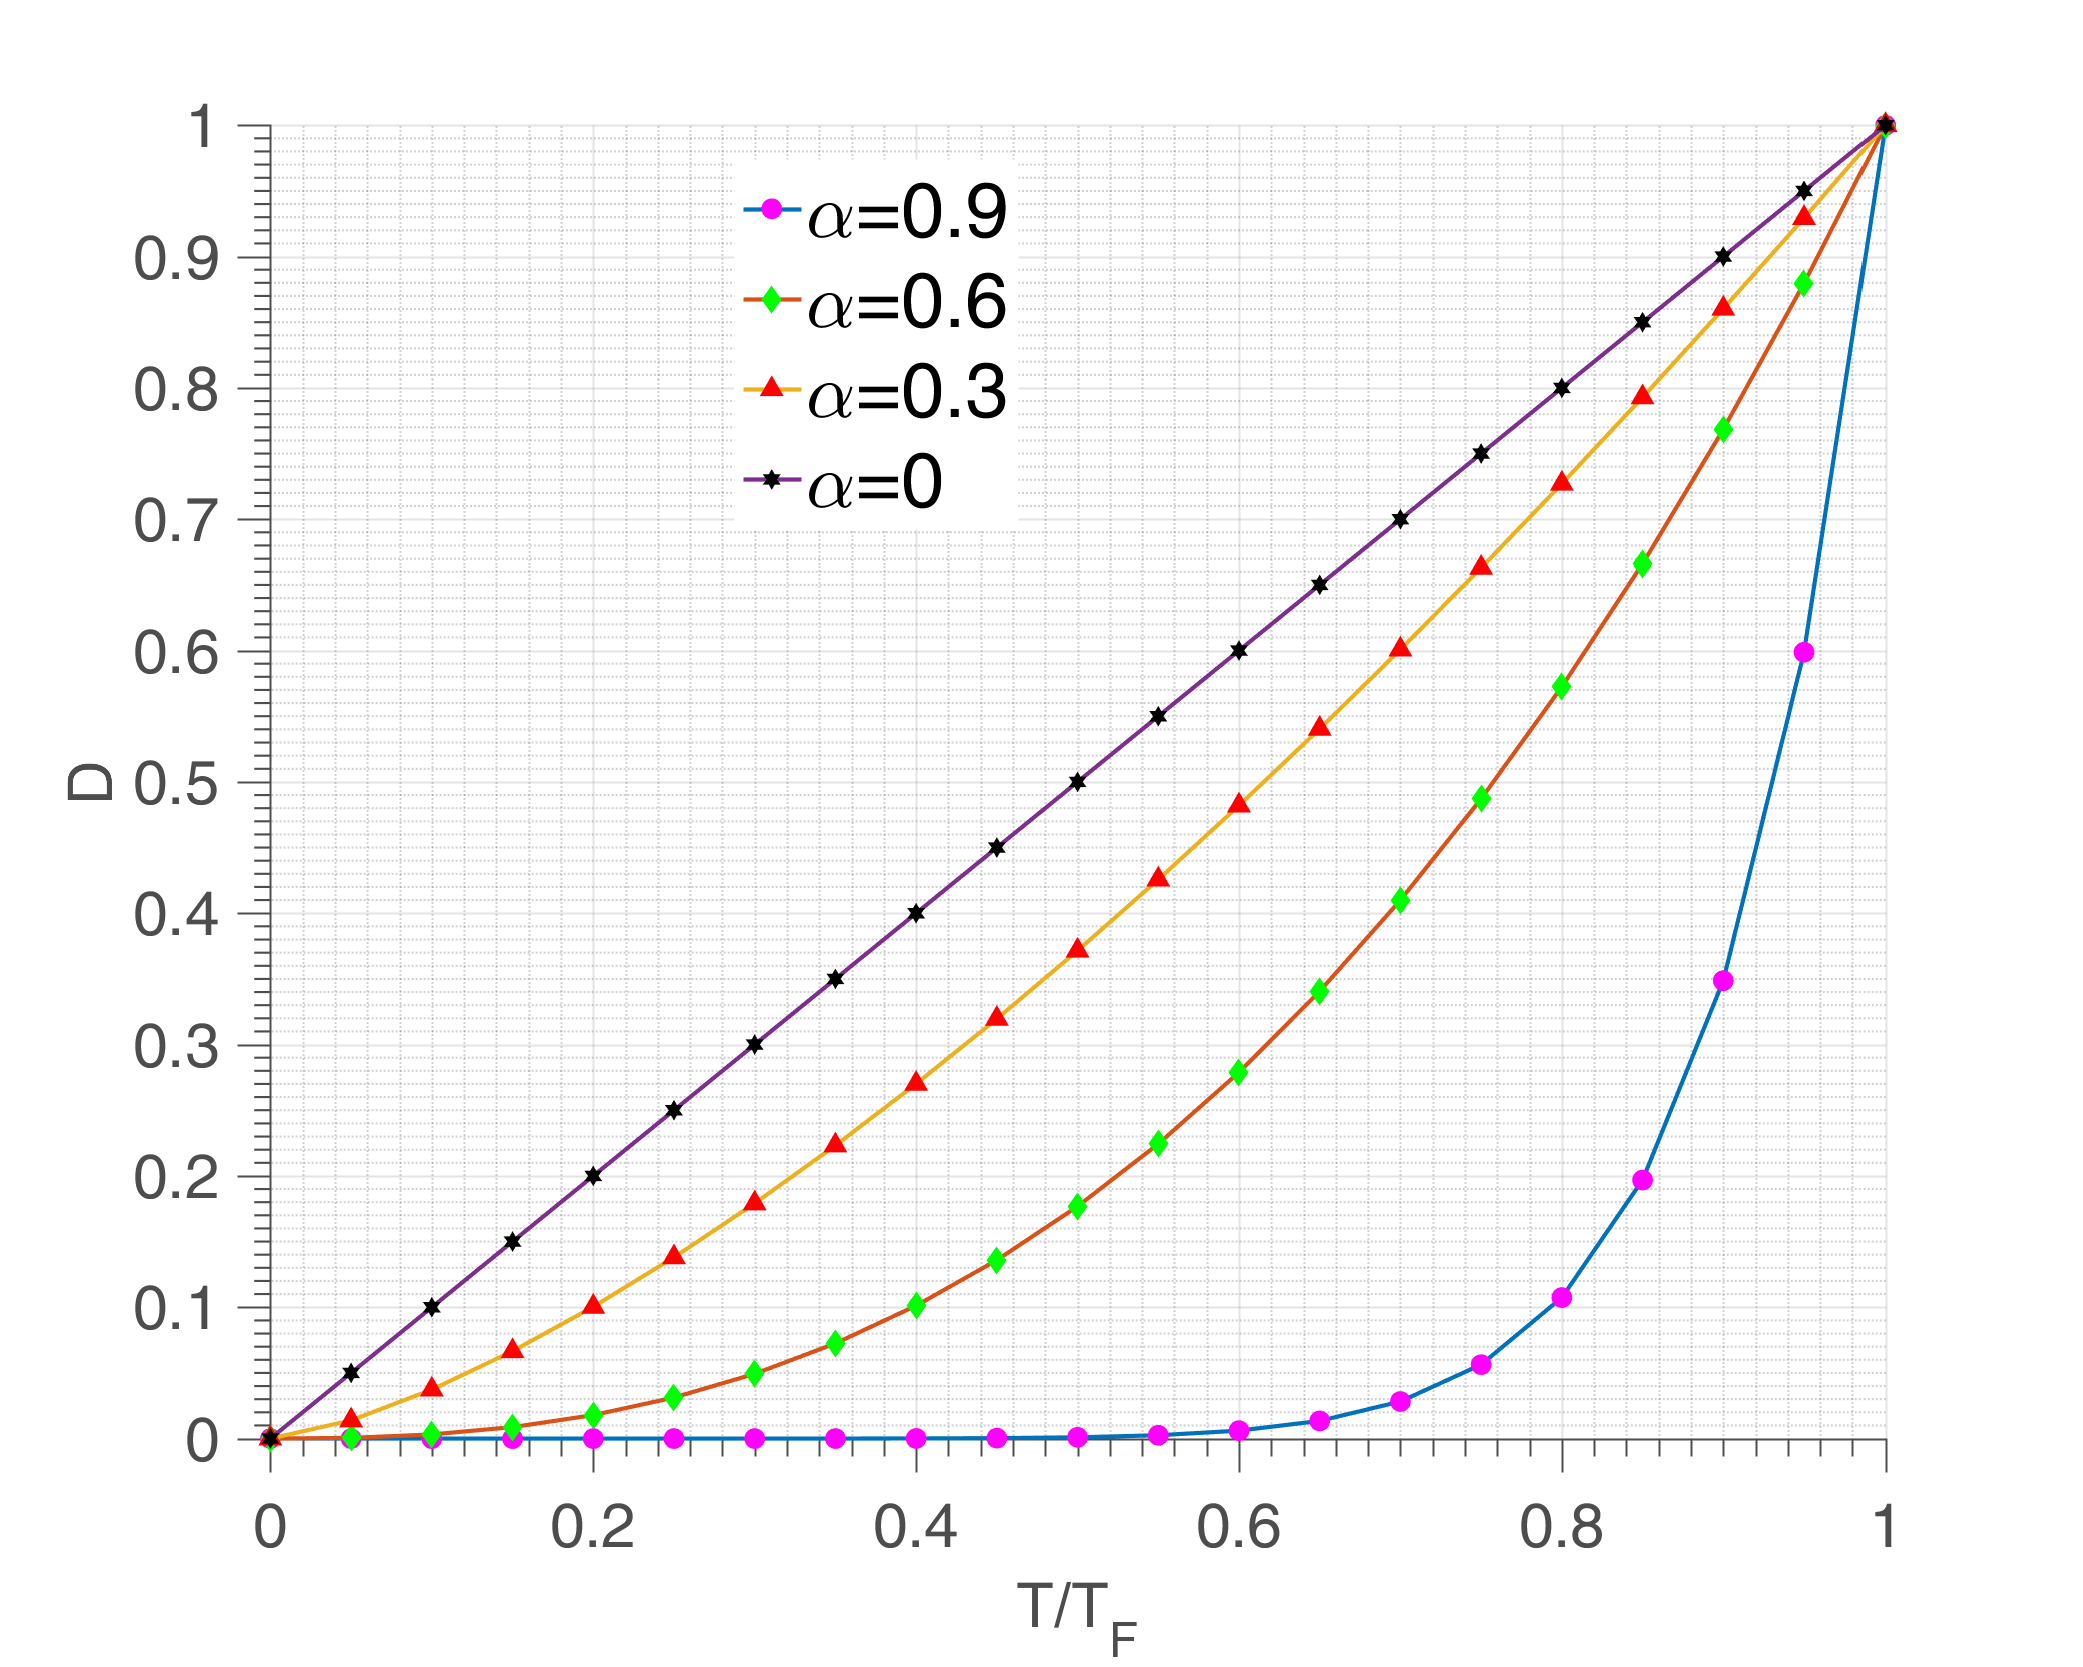
\includegraphics[width=\textwidth]{figures//alpha_accumulation_speed.png} 
	\caption{Influence of $\alpha$ on damage accumulation}
	\label{fig.alpha-accumulation-speed}
\end{figure}

To see the influence of sequence effect factor of $\alpha$, we first fix $\alpha=0.7$ for all tests to see the results. When $\alpha$ is fixed, it becomes denominator in the final expression of $N_F$(Eq.\eqref{eq.nf}) and has the same impact as $W_0$. We find out that the fatigue life of random loading is widely dispersed as in . In this case we need to use $\alpha=f(s_{min})$ which evolves with time to make large stress intensity deal more damage.




After analysis we find out that large stresses cause much more damage than the smaller stresses, even with $\alpha$ in Eq.\eqref{eq.alpha} the standard deviation is big. So it is necessary to include this major stress induced damage to our stress intensity parameter $\alpha$.

With the new $\alpha$ compared to Eq.\eqref{eq.alpha} we are able to calibrate our model better with the experimental results. 
$$\alpha=1-a\left(  \dfrac{\frac{1}{s_{min}}}{1-\frac{1}{s_{min}}} \right) ^{f(\beta)}.$$

We use the power $f(\beta)$ related to energy dissipation parameter $\beta$ to magnify large stress impact and minify lower stress damage.  The demonstration of major damage effect using  $f(\beta)$ is depicted in \figref{fig.sequenceours}. With larger value of $f(\beta)$, high stress causes more damage and low stress cause less damage.

\begin{figure}[!h]
	\centering
	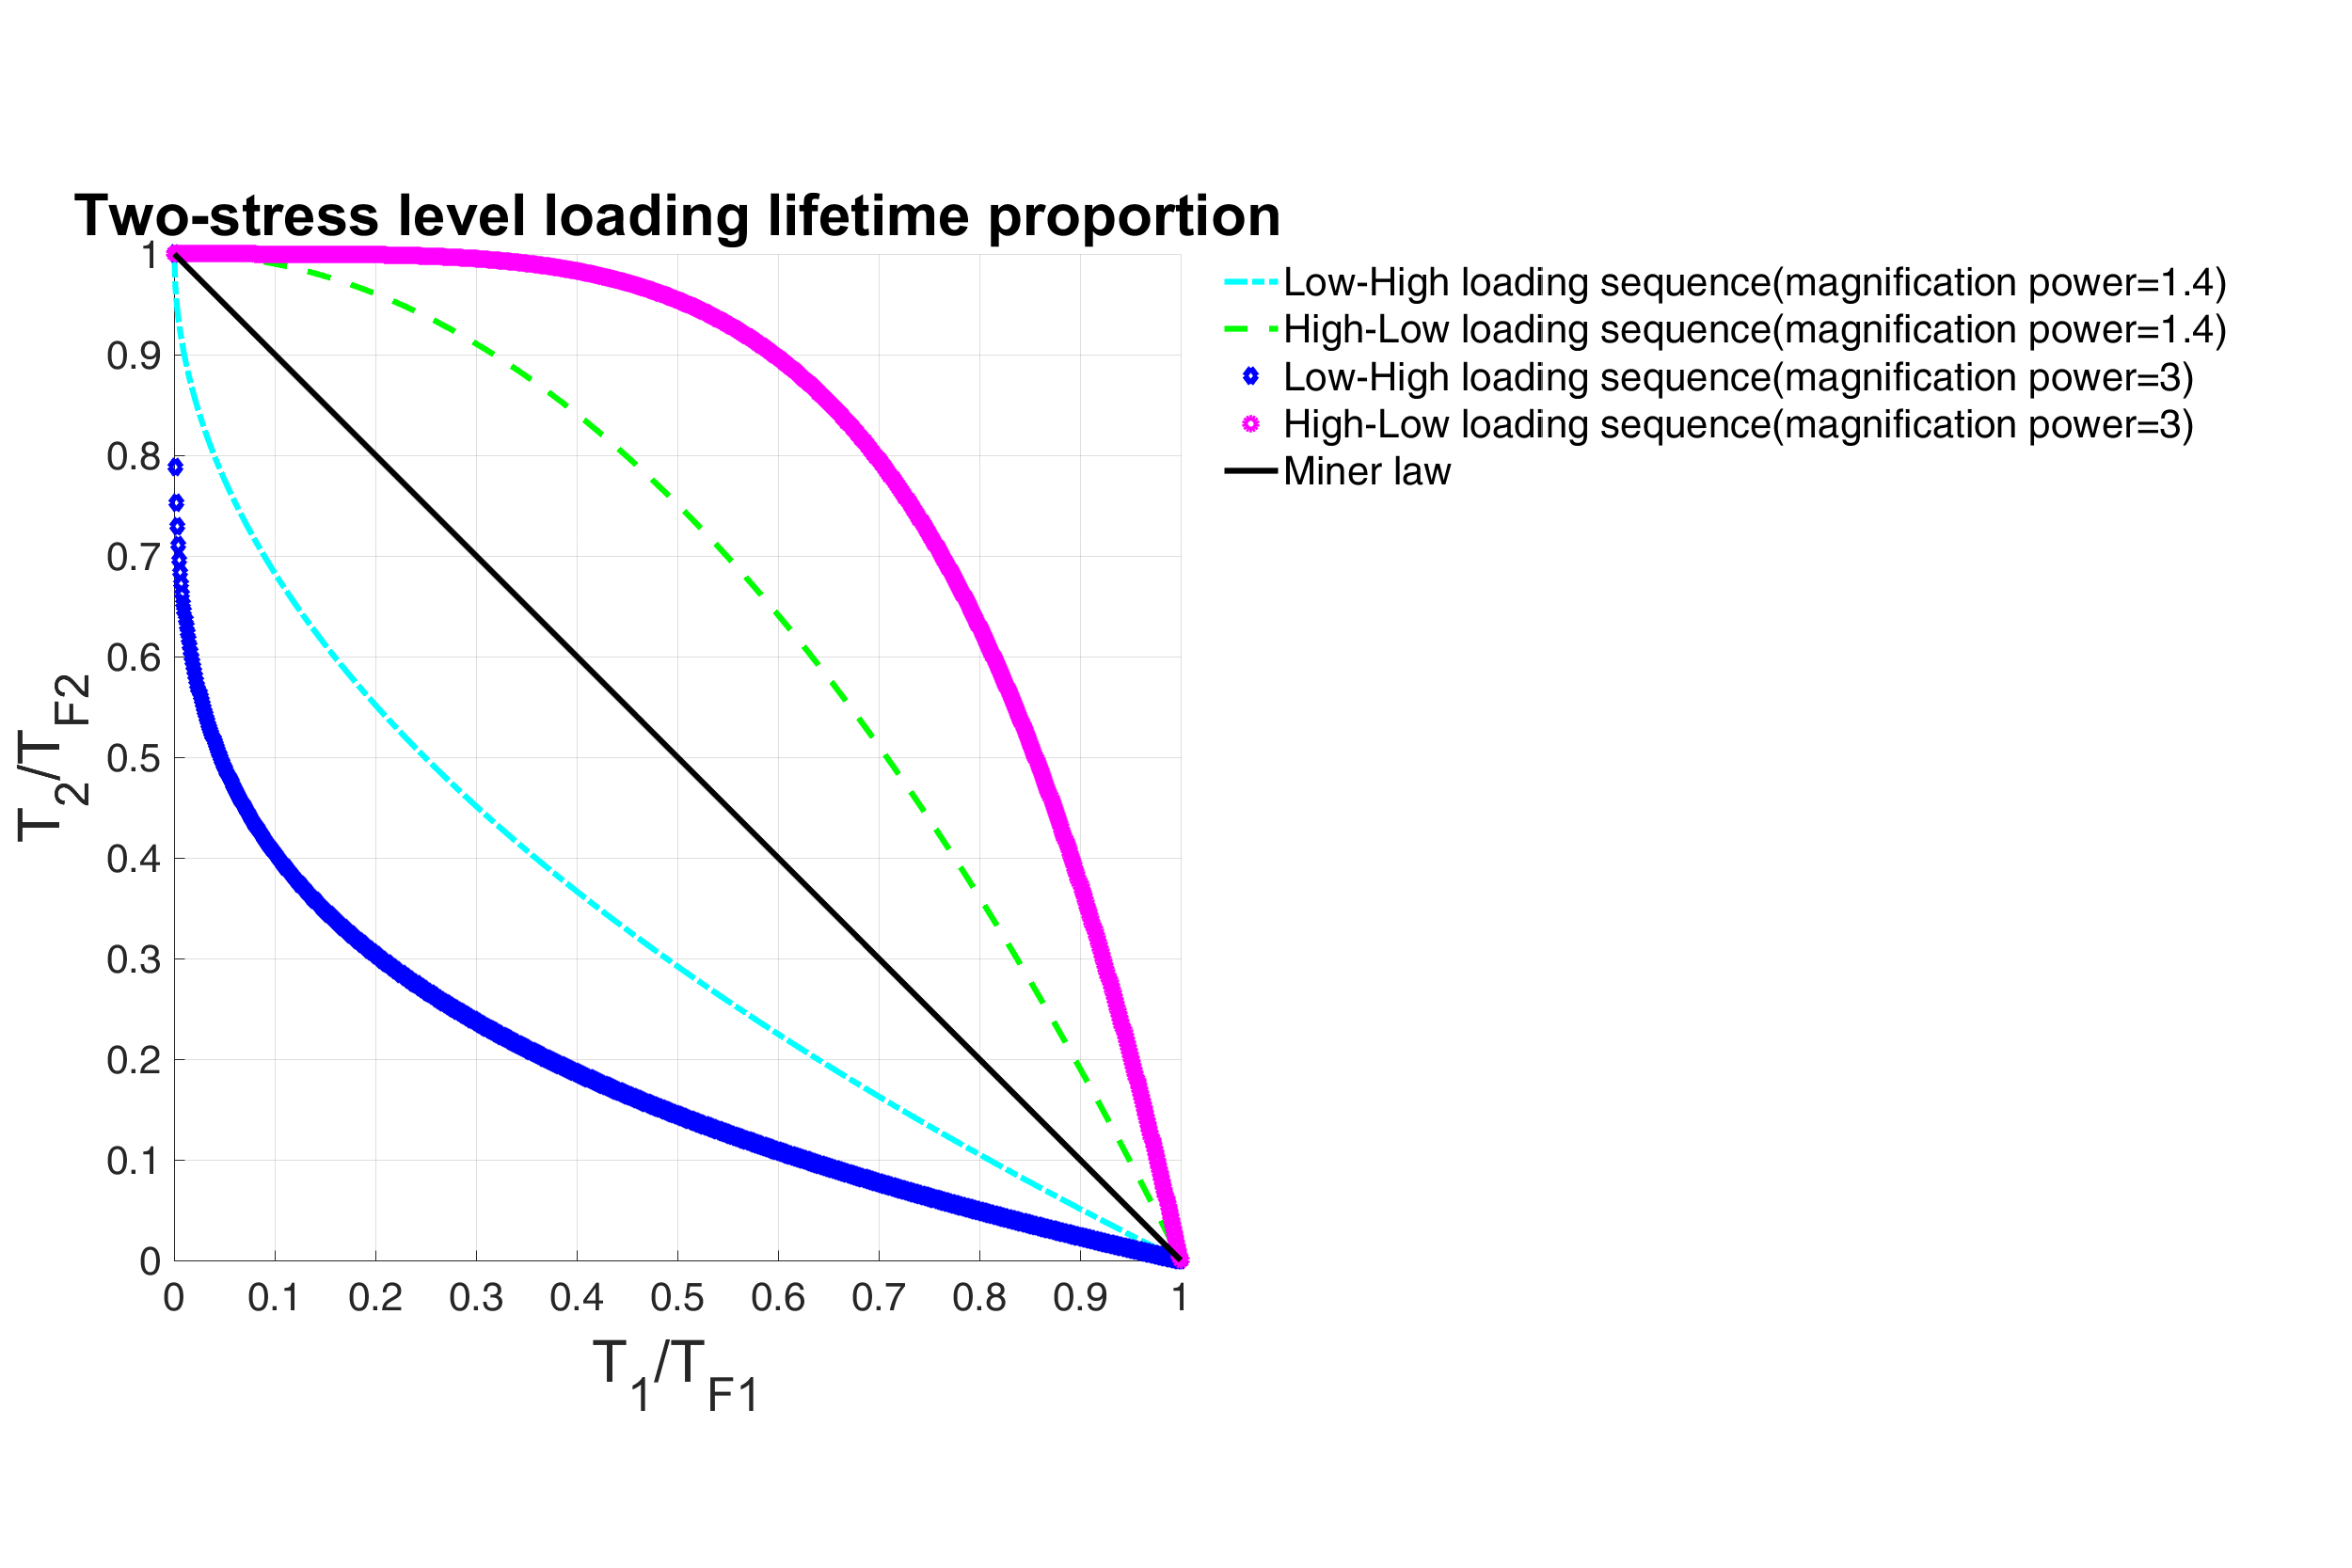
\includegraphics[width=0.8\textwidth]{figures//sequence_ours.png} 
	\caption{Major damage effect using different $f(\beta)$ on sequence effect figure}
	\label{fig.sequenceours}
\end{figure}

Here the power $f(\beta)$ and has anti-correlation with $T_F$ in low cycle fatigue regime but has positive correlation in high cycle fatigue regime. In our work the HCF is the regime we concern, so it is physically logical to give:
$$f(\beta)=\beta.$$
which yields the new expression of $\alpha$ in Eq.\eqref{eq.newalpha}:
\begin{equation}
\alpha=1-a\left(  s_{min}-1 \right) ^{-\beta}.
\label{eq.newalpha}
\end{equation}

The larger value of $S_{max}$ causes more damage in the presence of the power $\beta$, leading to faster increase of $$(1-\alpha)=a\left(  \dfrac{\frac{1}{s_{min}}}{1-\frac{1}{s_{min}}} \right) ^\beta$$ 
which causes faster damage accumulation. We can also see this effect in \figref{fig.alpha}. However, $\alpha$ must be positive. 

The parameters used in the fitting process are shown in Tab.\ref{tab.cetim.para}. 
The deviatoric stress $S_{max}$, above which the damage is magnified,  is determined from:
$$S_{large}=\dfrac{1}{2}\Sigma_y.$$ 
This major damage effect can be seen in \figref{fig.SmaxSequence}.

\begin{figure}[!h]
	\centering
	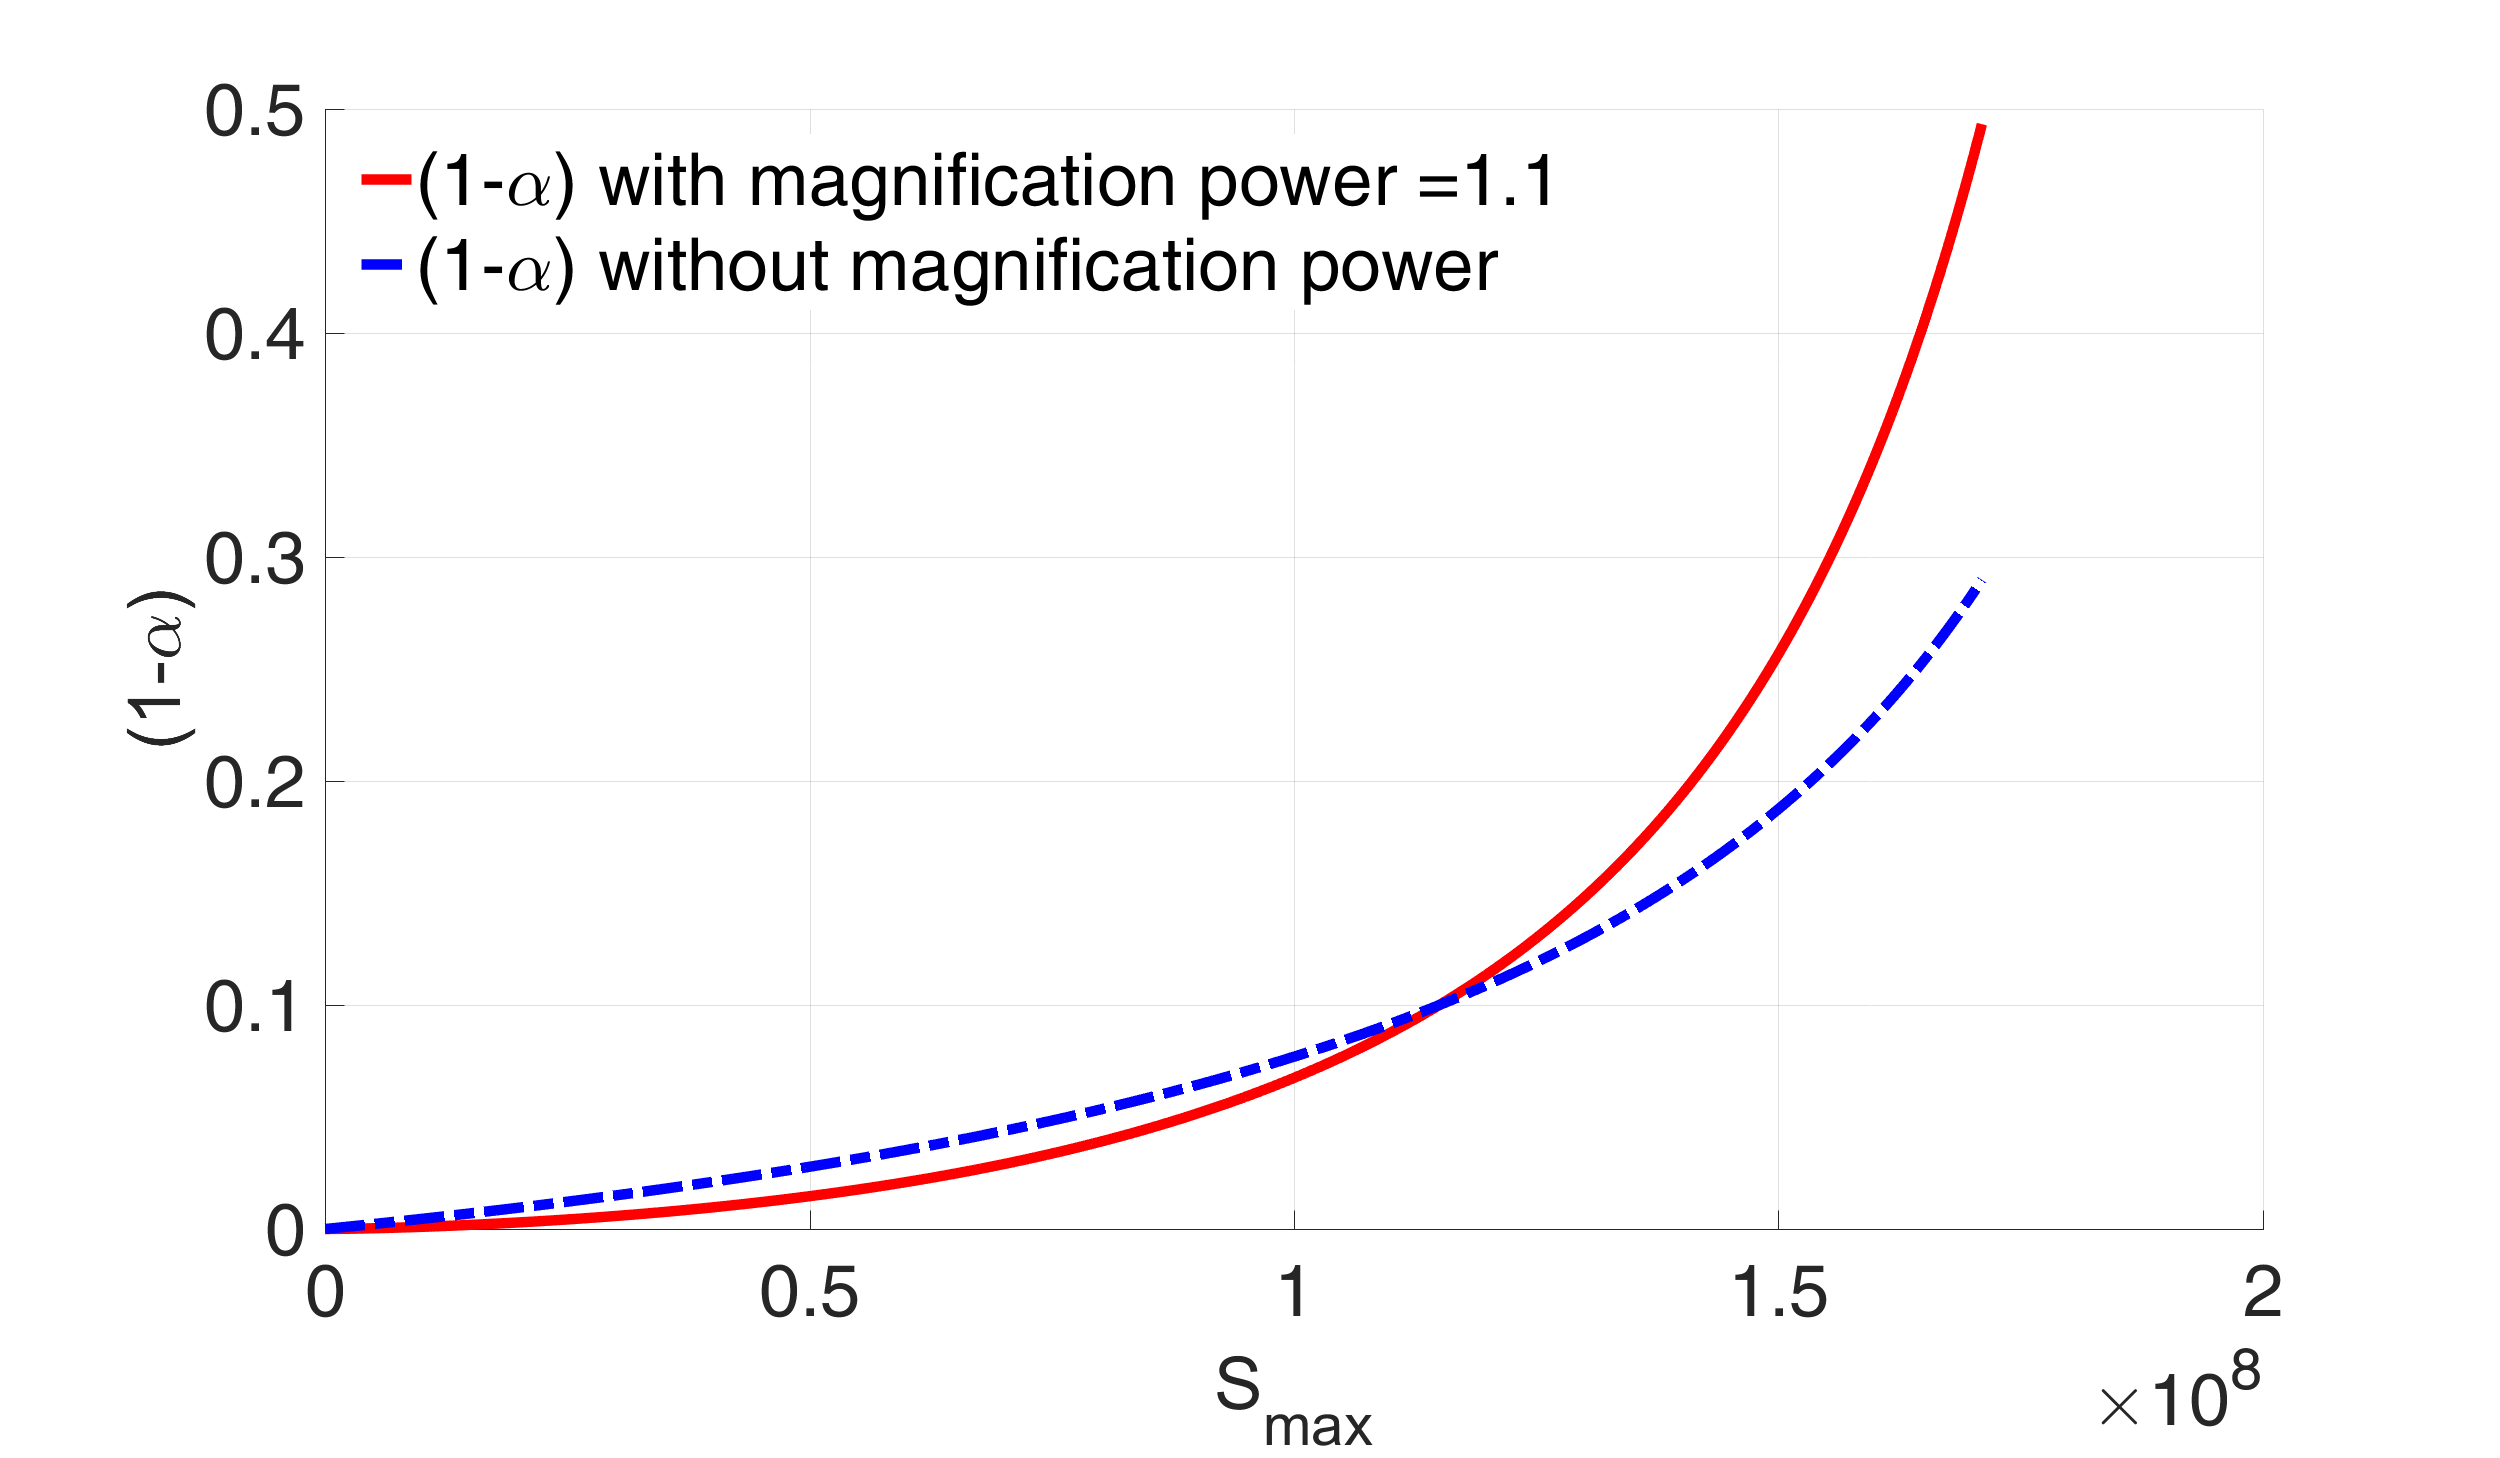
\includegraphics[width=\textwidth]{figures//alp_Smax_fb.png} 
	\caption{(1-$\alpha$) term with and without the magnification power $\beta$}
	\label{fig.SmaxSequence}
\end{figure}

The reference parameters value we use are in Tab.\ref{tab.cetim.alp}.  
\begin{table}[!h]
	\centering
	\begin{tabular}{lrrrr}
		\hline
\textbf{Constant $\alpha$} & \textbf{$W_0$(MPa)} & \textbf{$\lambda$} & \textbf{$\beta$}  & \textbf{$\alpha$}\\
		      & 326.9         & 0.1               & 1.1            & 0.7                         \\ \hline
\textbf{Changing $\alpha$} & \textbf{$W_0$(MPa)} & \textbf{$\lambda$} & \textbf{$\beta$}  & \textbf{$a$}\\
		      & 326.9         & 0.1               & 1.1            & 0.1                         \\ \hline
	\end{tabular}
	\caption{The parameters in 1D cyclic and random loading on AW-6106 T6
		aluminum fatigue tests by Cetim}
	\label{tab.cetim.alp}
\end{table}

The best fitted results with constant $\alpha$ are shown in \figref{fig.Cetimerralpfix}. The dispersion is relatively large. In conclusion, we are not able to predict the random stress amplitude fatigue life with fixed $\alpha$, because random stresses not only cause different energy dissipations, but also have influence on damage accumulation speed, so we have to update the value of $\alpha$ at each time step. 

\begin{figure}[!h]
	\centering
	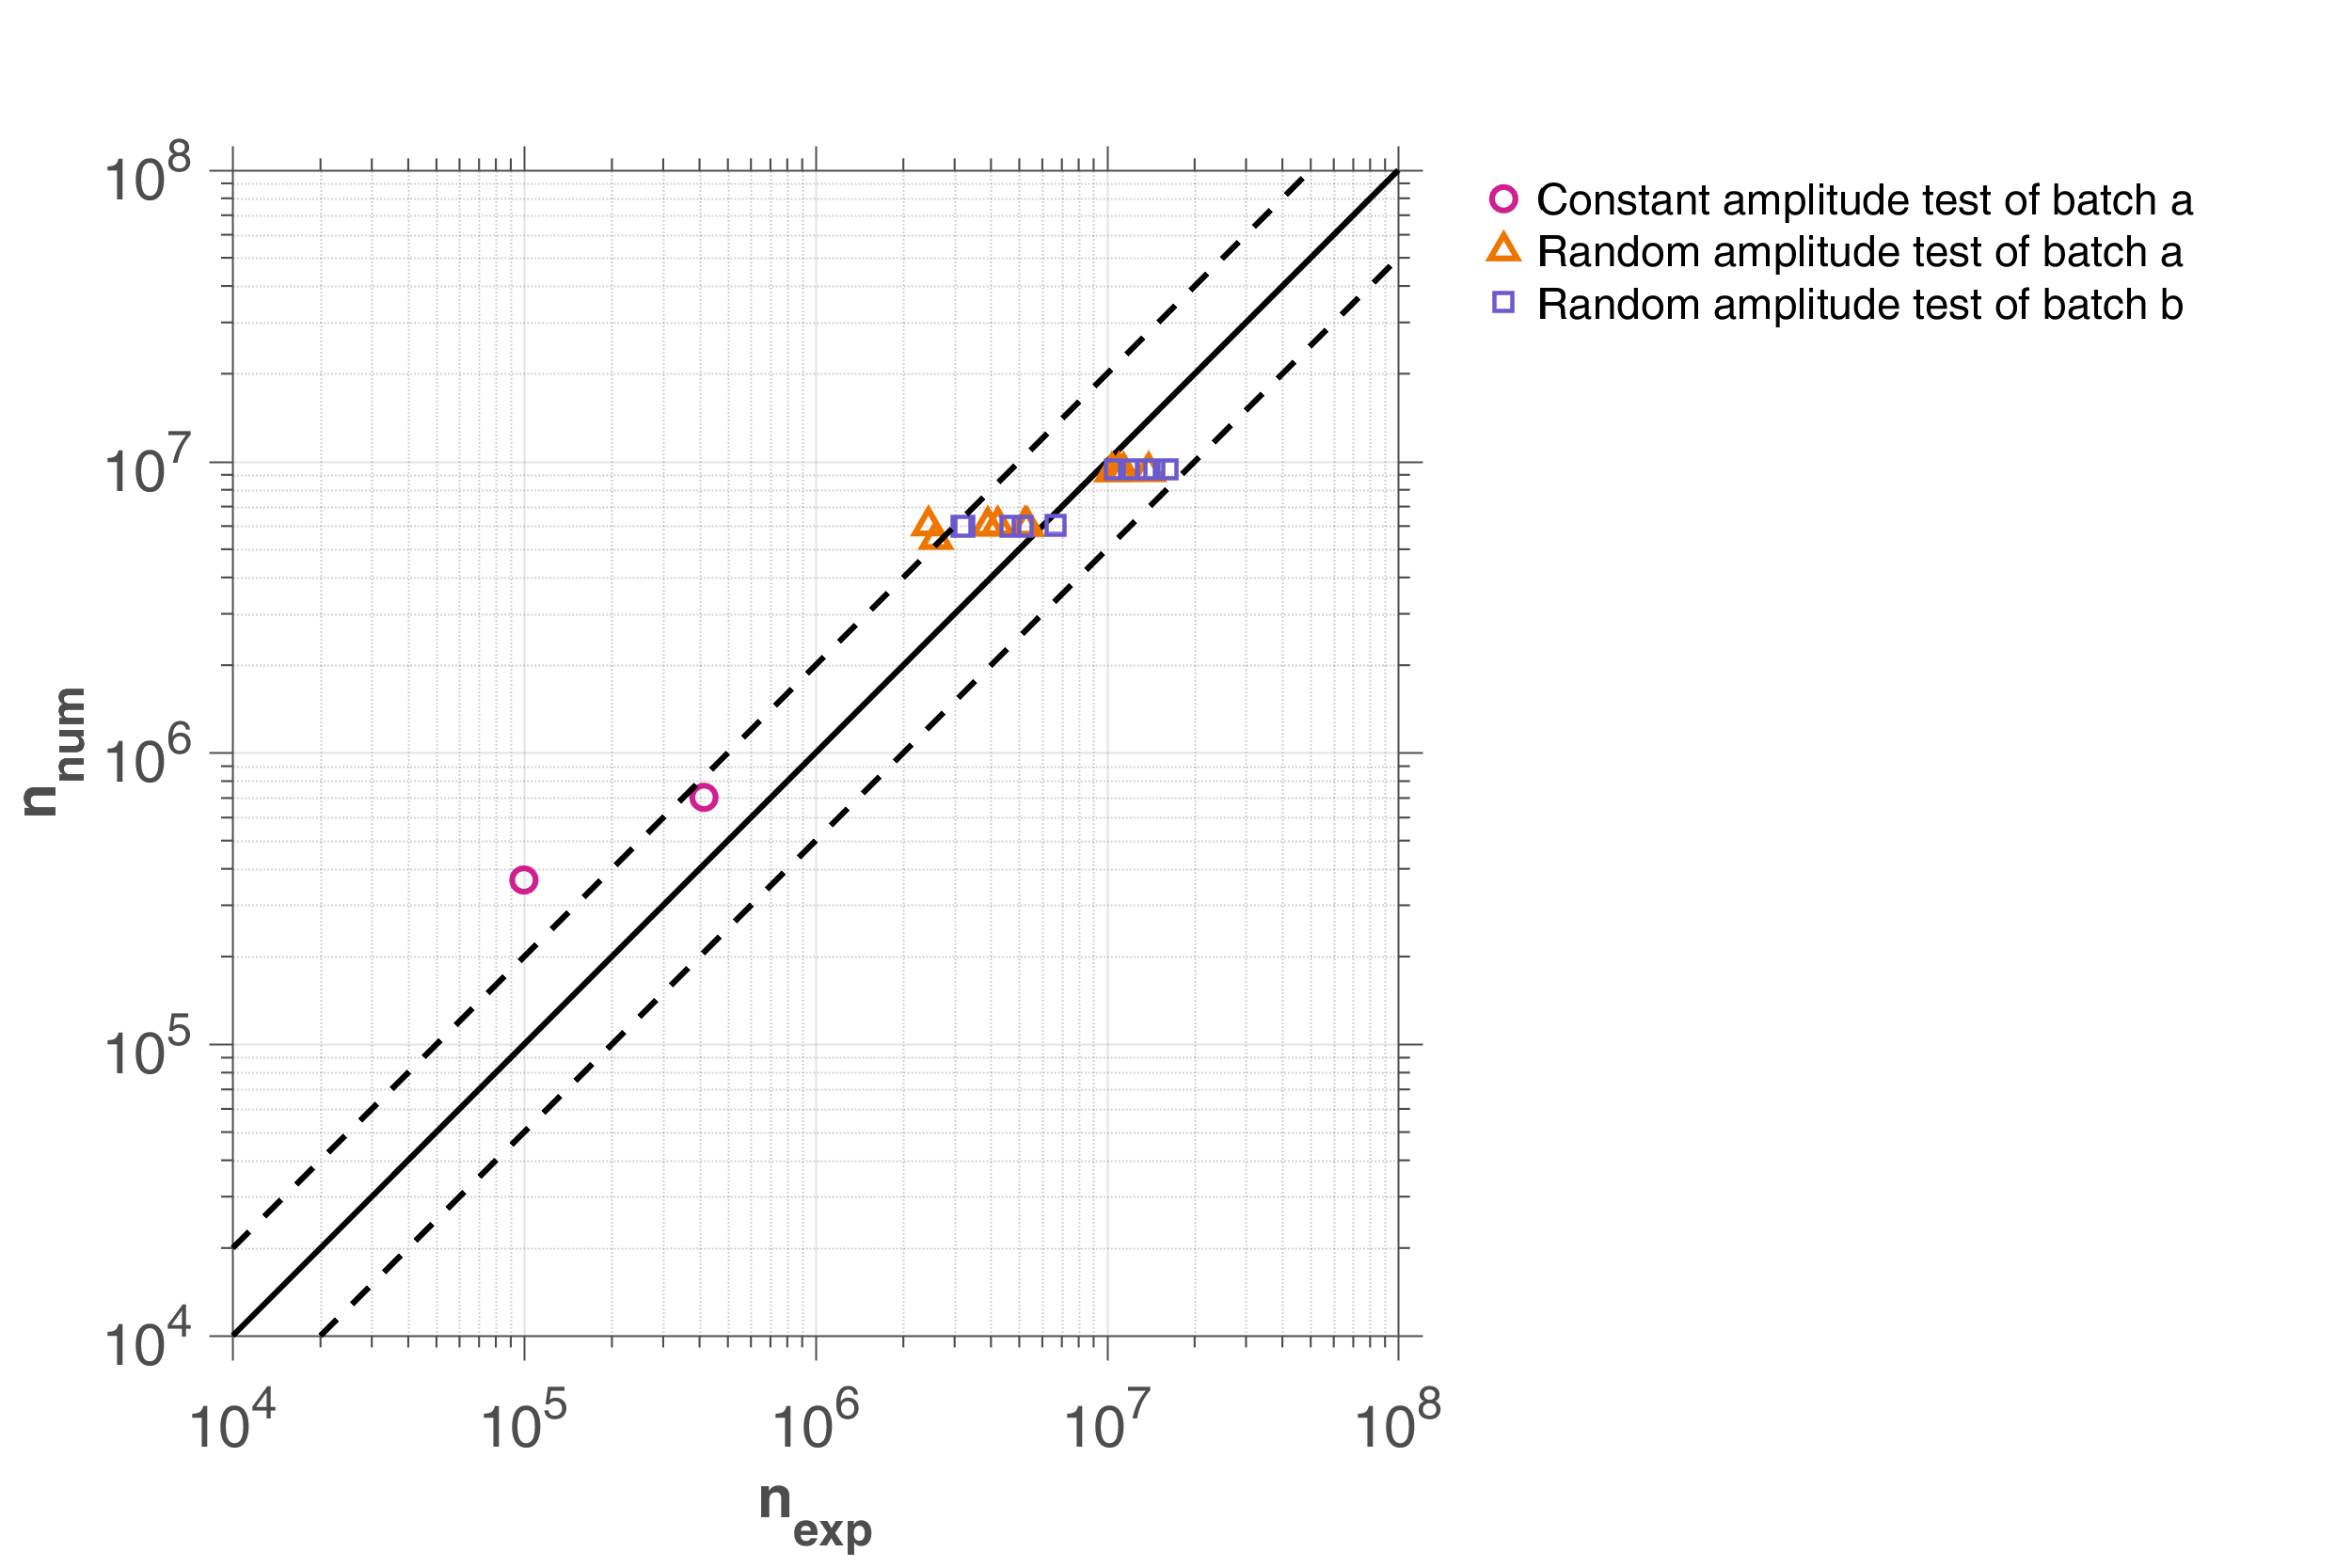
\includegraphics[width=\textwidth]{figures//Cetim_err_alpfix.png} 
	\caption{Comparison between experimental and numerical results of 1D cyclic and random loading on aluminum fatigue tests by Cetim with constant $\alpha$}
	\label{fig.Cetimerralpfix}
\end{figure}

We can find that the numerical results are satisfactory with magnification power. The dispersion figure with distinction of major damage is depicted in \figref{fig.Cetimerr}. Here it is necessary to control the parameter $a$ to make sure $\alpha>0$ in the most severe situation.

\begin{figure}[!h]
	\centering
	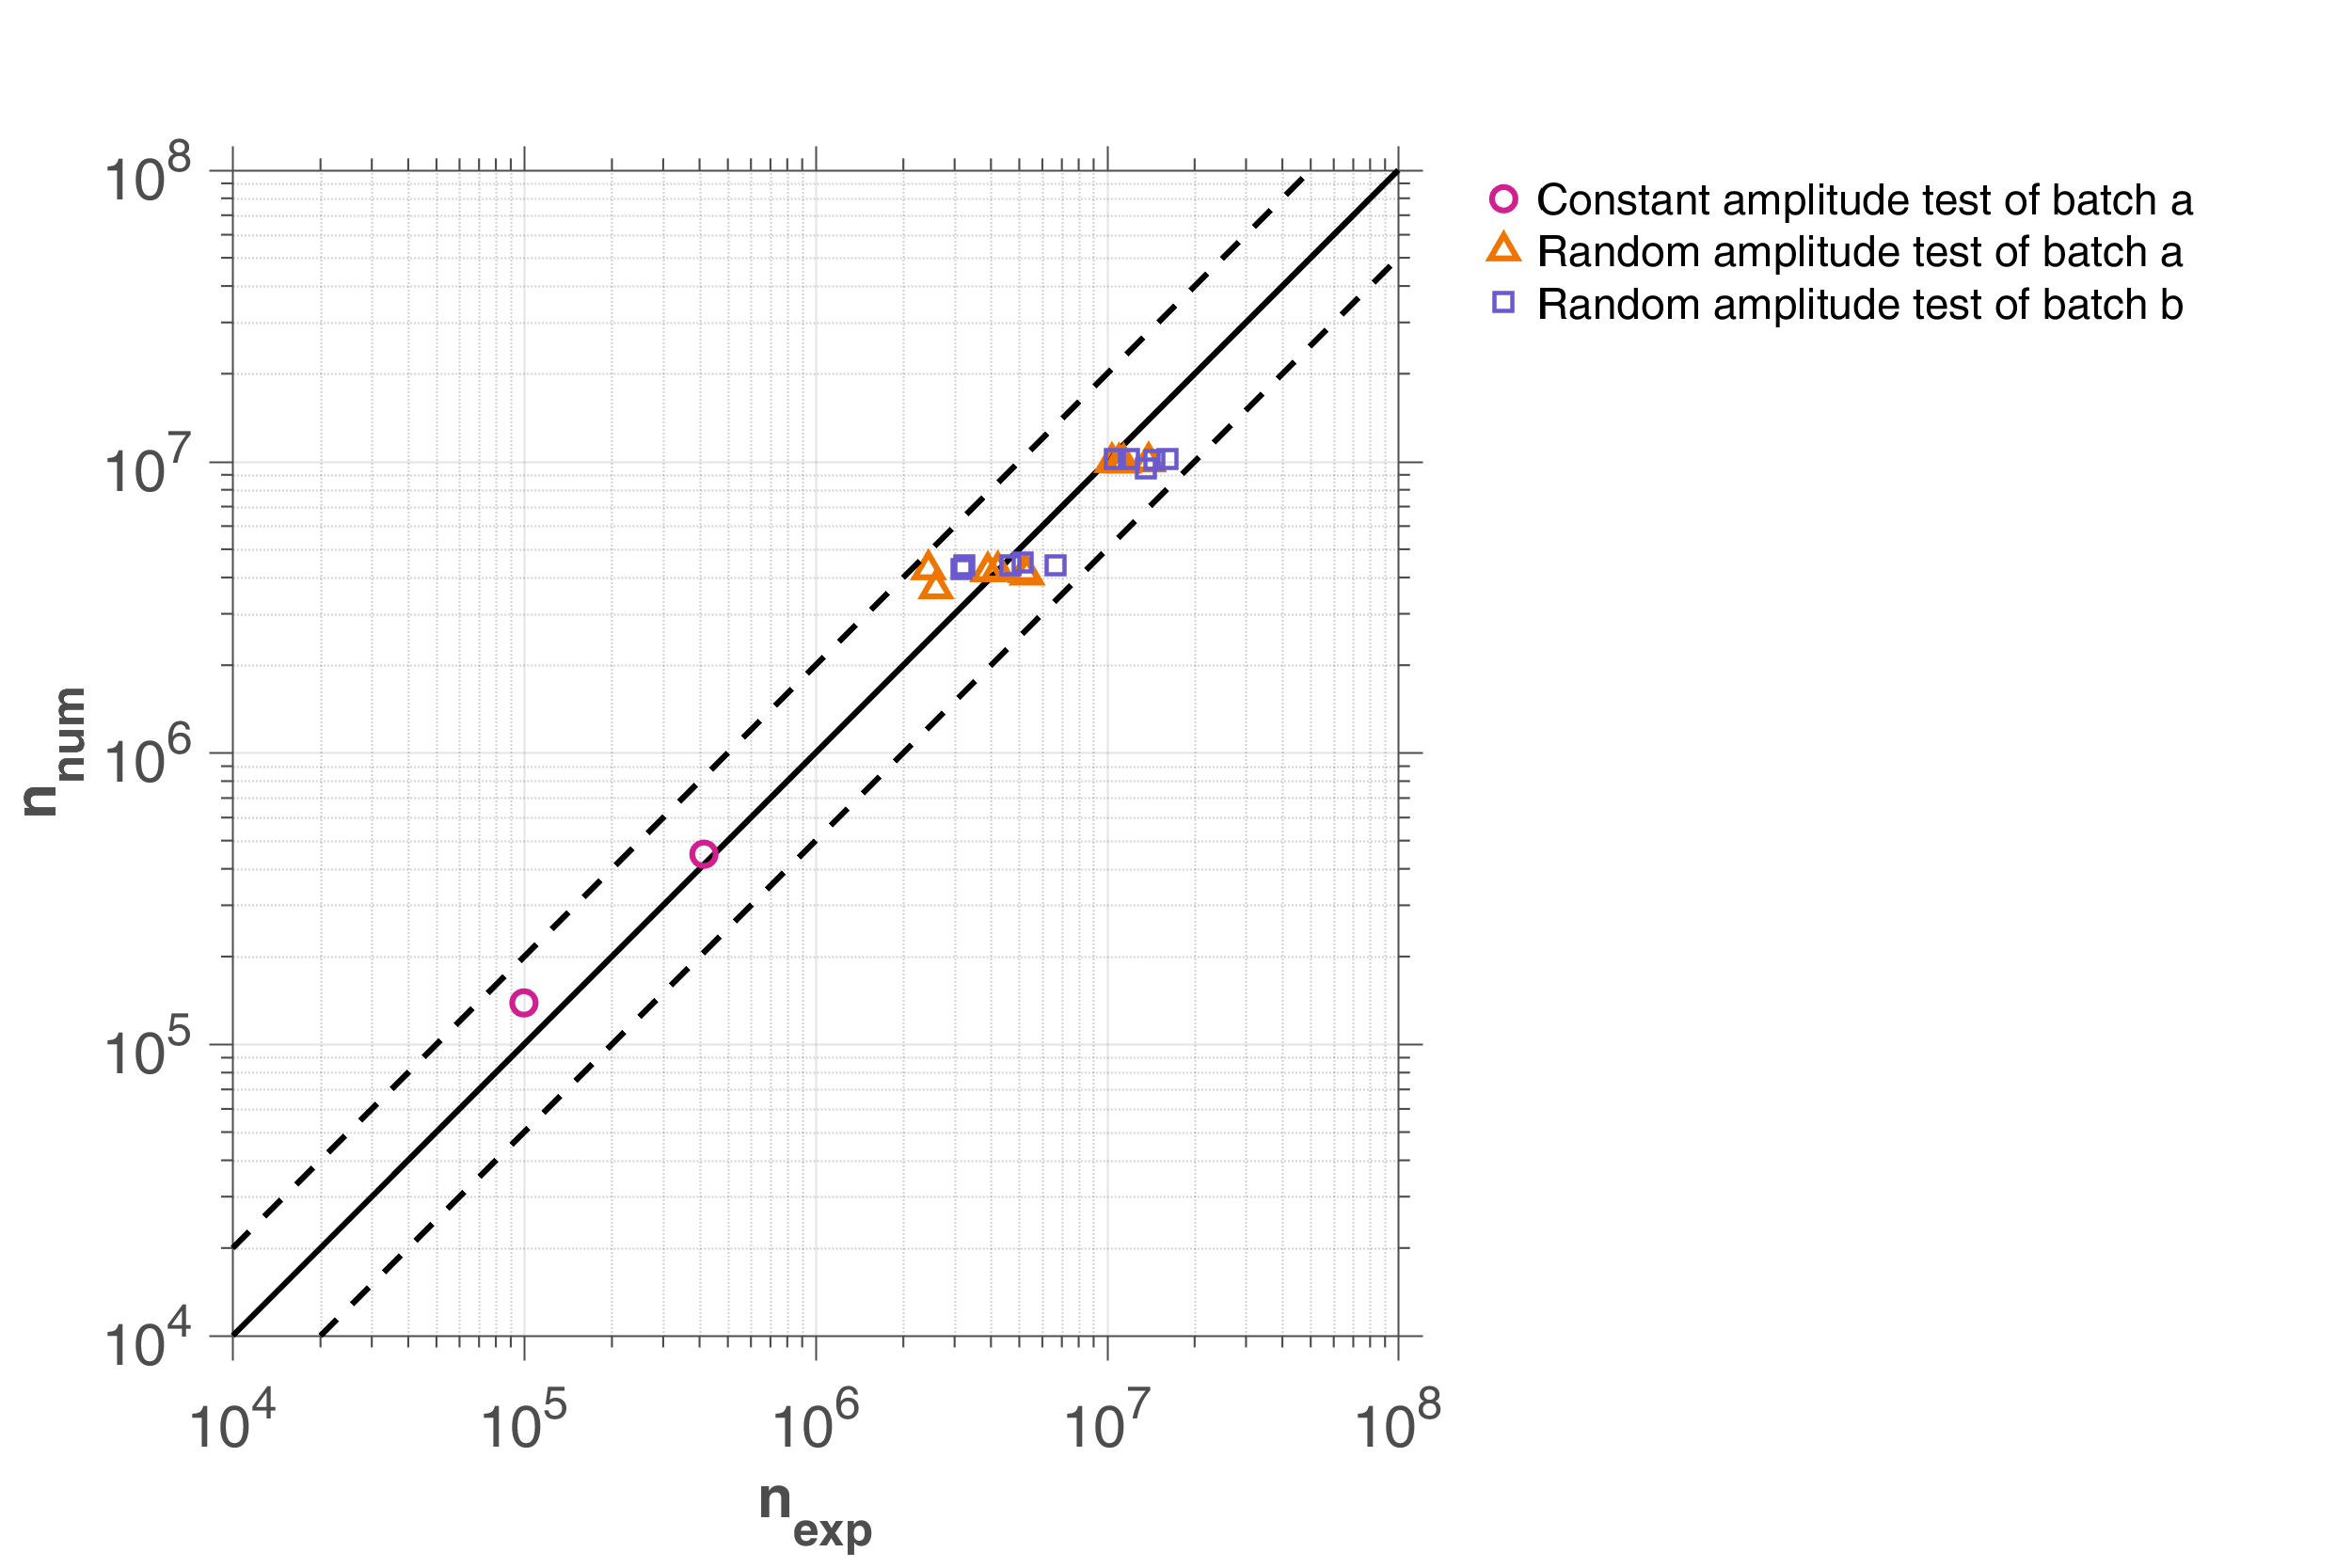
\includegraphics[width=\textwidth]{figures//Cetim_err.png} 
	\caption{Comparison between experimental and numerical results of 1D cyclic and random loading on aluminum fatigue tests by Cetim}
	\label{fig.Cetimerr}
\end{figure}

\clearpage
\subsection{Experimental validation of the model on 30NCD16 steel}
\subsubsection{Presentation of steel 30 NCD 16}
Tests with blocks of loading from database are compared to our model predictions. The material for testing is steel 30NCD16. The mechanical characteristics relating to each lot were determined by Dubar \cite{Dubar1992} by effecting
monotonic tensile test batch. He eventually define ``average material" one who has
characteristics listed in Table. \ref{30ncdchar}:

\begin{table}[!h]
	\centering
	\begin{tabular}{|c|c|c|c|l|c|}
		\hline
		\textbf{$\sigma_{y0.02\%}${[}MPa{]}} & \textbf{$\sigma_{y0.2\%}${[}MPa{]}} & \textbf{$\sigma_u${[}MPa{]}} & \textbf{$\sigma_{-1}${[}MPa{]}} & \textbf{$\tau_{-1}${[}MPa{]}} & \textbf{$E${[}GPa{]}}\\ \hline
		895                                  & 1080                                & 1200                         & 690                             & \multicolumn{1}{c|}{428}     & 191 \\ \hline
	\end{tabular}
	\caption{Mechanical and dynamic characteristics of 30NCD16 steel \cite{Dubar1992}}
	\label{30ncdchar}
\end{table}

\subsubsection{Fatigue tests performed by Dubar on steel 30 NCD 16}
Tests carried out under simple bending and torsional stresses are grouped together in
Table. \ref{bendingr1} and \ref{torsionR1}.

\begin{table}[!h]
	\centering
\begin{tabular}{|c|c|c|c|}
	\hline
	\begin{tabular}[c]{@{}c@{}}Bending Tests\\ (R=-1)\end{tabular} & \begin{tabular}[c]{@{}c@{}}N\\ {[}Cycles{]}\end{tabular} & \begin{tabular}[c]{@{}c@{}}$\sigma_{x,m}$\\ {[}MPa{]}\end{tabular} & \begin{tabular}[c]{@{}c@{}}$\sigma_{x,a}$\\ {[}MPa{]}\end{tabular} \\ \hline
	1 & 51000 & 0 & 820 \\  \hline
	2 & 80000 & 0 & 795 \\  \hline
	3 & 90000 & 0 & 790 \\  \hline
	4 & 95000 & 0 & 785 \\  \hline
	5 & 100000 & 0 & 780 \\  \hline
	6 & 120000 & 0 & 765 \\  \hline
	7 & 140000 & 0 & 752 \\  \hline
	8 & 200000 & 0 & 725 \\  \hline
	9 & 210000 & 0 & 720 \\  \hline
	10 & 230000 & 0 & 715 \\  \hline
	11 & 250000 & 0 & 708 \\ \hline  \hline
	12 & 51000 & 450 & 640 \\  \hline
	13 & 140000 & 450 & 620 \\   \hline
	14 & 120000 & 290 & 695 \\  \hline
	15 & 250000 & 290 & 660 \\ \hline
\end{tabular}
	\caption{$30 NCD 16$ steel fully reversed bending tests \cite{Dubar1992}}
	\label{bendingr1}
\end{table}

\begin{table}[!h]
	\centering
\begin{tabular}{|c|c|c|}
	\hline
	\begin{tabular}[c]{@{}c@{}}Torsion Tests\\ (R=-1)\end{tabular} & \begin{tabular}[c]{@{}c@{}}N\\ {[}Cycles{]}\end{tabular} & \begin{tabular}[c]{@{}c@{}}$\tau_{xy,a}$\\ {[}MPa{]}\end{tabular} \\ \hline
	16 & 51000 & 527 \\ \hline
	17 & 80000 & 505 \\ \hline
	18 & 90000 & 500 \\ \hline
	19 & 95000 & 497 \\ \hline
	20 & 100000 & 495 \\ \hline
	21 & 120000 & 482 \\ \hline
	22 & 140000 & 470 \\ \hline
	23 & 200000 & 450 \\ \hline
	24 & 210000 & 446 \\ \hline
	25 & 230000 & 445 \\ \hline
	26 & 250000 & 440 \\ \hline
\end{tabular}
	\caption{$30 NCD 16$ steel fully reversed torsion tests \cite{Dubar1992}}
	\label{torsionR1}
\end{table}

The results of combined bending-torsion tests in phase with or without mean stress $\sigma_{x,m}$ are given in the following table:
\begin{table}[!h]
	\centering
\begin{tabular}{|c|c|c|c|c|}
	\hline
	\begin{tabular}[c]{@{}c@{}}Bending Tests\\ (R=-1)\end{tabular} & \begin{tabular}[c]{@{}c@{}}N\\ {[}Cycles{]}\end{tabular} & \begin{tabular}[c]{@{}c@{}}$\sigma_{x,m}$\\ {[}MPa{]}\end{tabular} & \begin{tabular}[c]{@{}c@{}}$\sigma_{x,a}$\\ {[}MPa{]}\end{tabular} & \begin{tabular}[c]{@{}c@{}}$\tau_{xy,a}$\\ {[}MPa{]}\end{tabular} \\ \hline
	27 & 51000 & 0 & 600 & 335 \\ \hline
	28 & 80000 & 0 & 548 & 306 \\ \hline
	29 & 90000 & 290 & 0 & 460 \\ \hline
	30 & 95000 & 450 & 0 & 460 \\ \hline
	31 & 100000 & 450 & 0 & 430 \\ \hline
	32 & 120000 & 450 & 490 & 285 \\ \hline
	33 & 140000 & 290 & 500 & 290 \\ \hline
\end{tabular}
	\caption{$30 NCD 16$ steel bending-torsion tests \cite{Dubar1992}}
\label{tab.30ncd16bt}
\end{table}

\subsubsection{Identification of model parameters for steel 30 NCD 16}
Indeed, the identification of the parameters consists in minimizing the relative difference between the experimental lifetimes and calculated for purely alternating bending tests (R = -1). This is clearly indicated in figure (3.13) by obtaining a good correlation between these different lifetimes
\begin{table}[!h]
	\centering
	\begin{tabular}{|c|c|c|}
		\hline
		\textbf{$\beta$} & \textbf{$\lambda$}  & \textbf{$W_0/a$}  \\ \hline
	                    1.85        & 0.85           & 440e9       \\ \hline
	\end{tabular}
	\caption{Parameter identification of 30NCD16 steel}
	\label{30ncdpara}
\end{table}

\begin{figure}[!h]
	\centering
	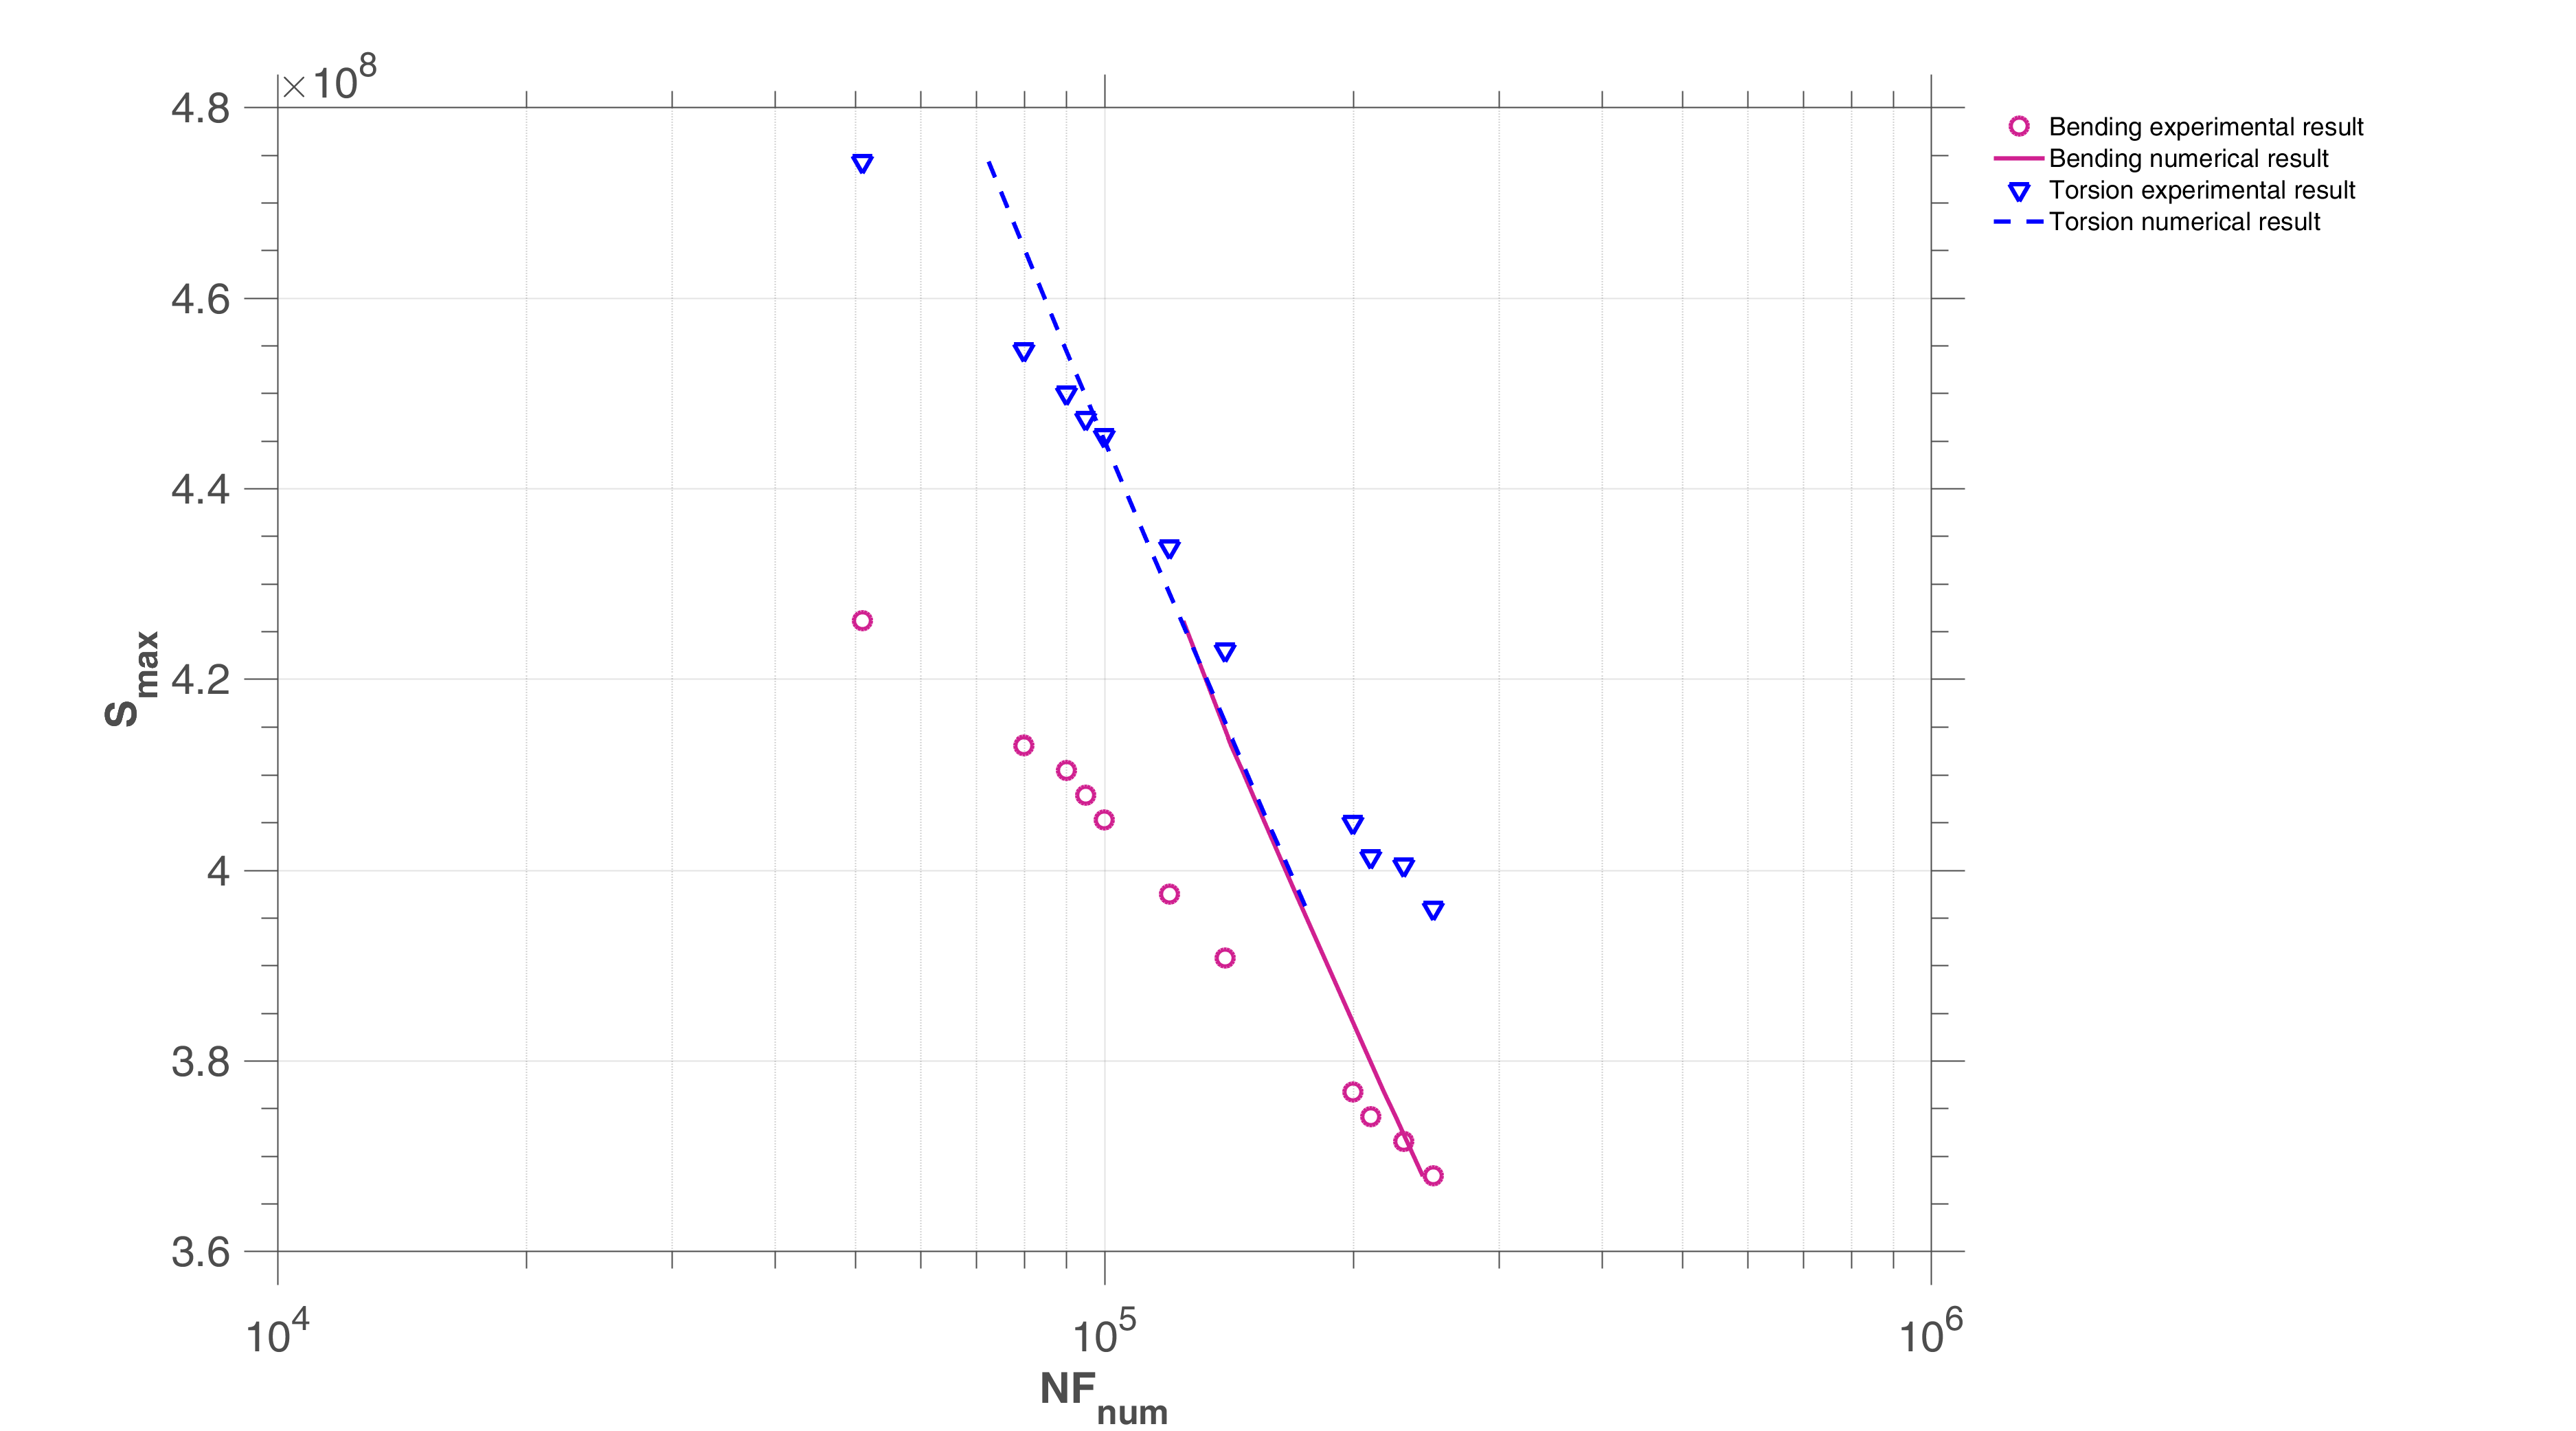
\includegraphics[width=\textwidth]{figures//bt1D_30NCD16_sn.png} 
	\caption{Bending and torsion tests on 30NCD16(R=-1)}
	\label{fig.bt1D30NCD16sn}
\end{figure}
\begin{figure}[!h]
	\centering
	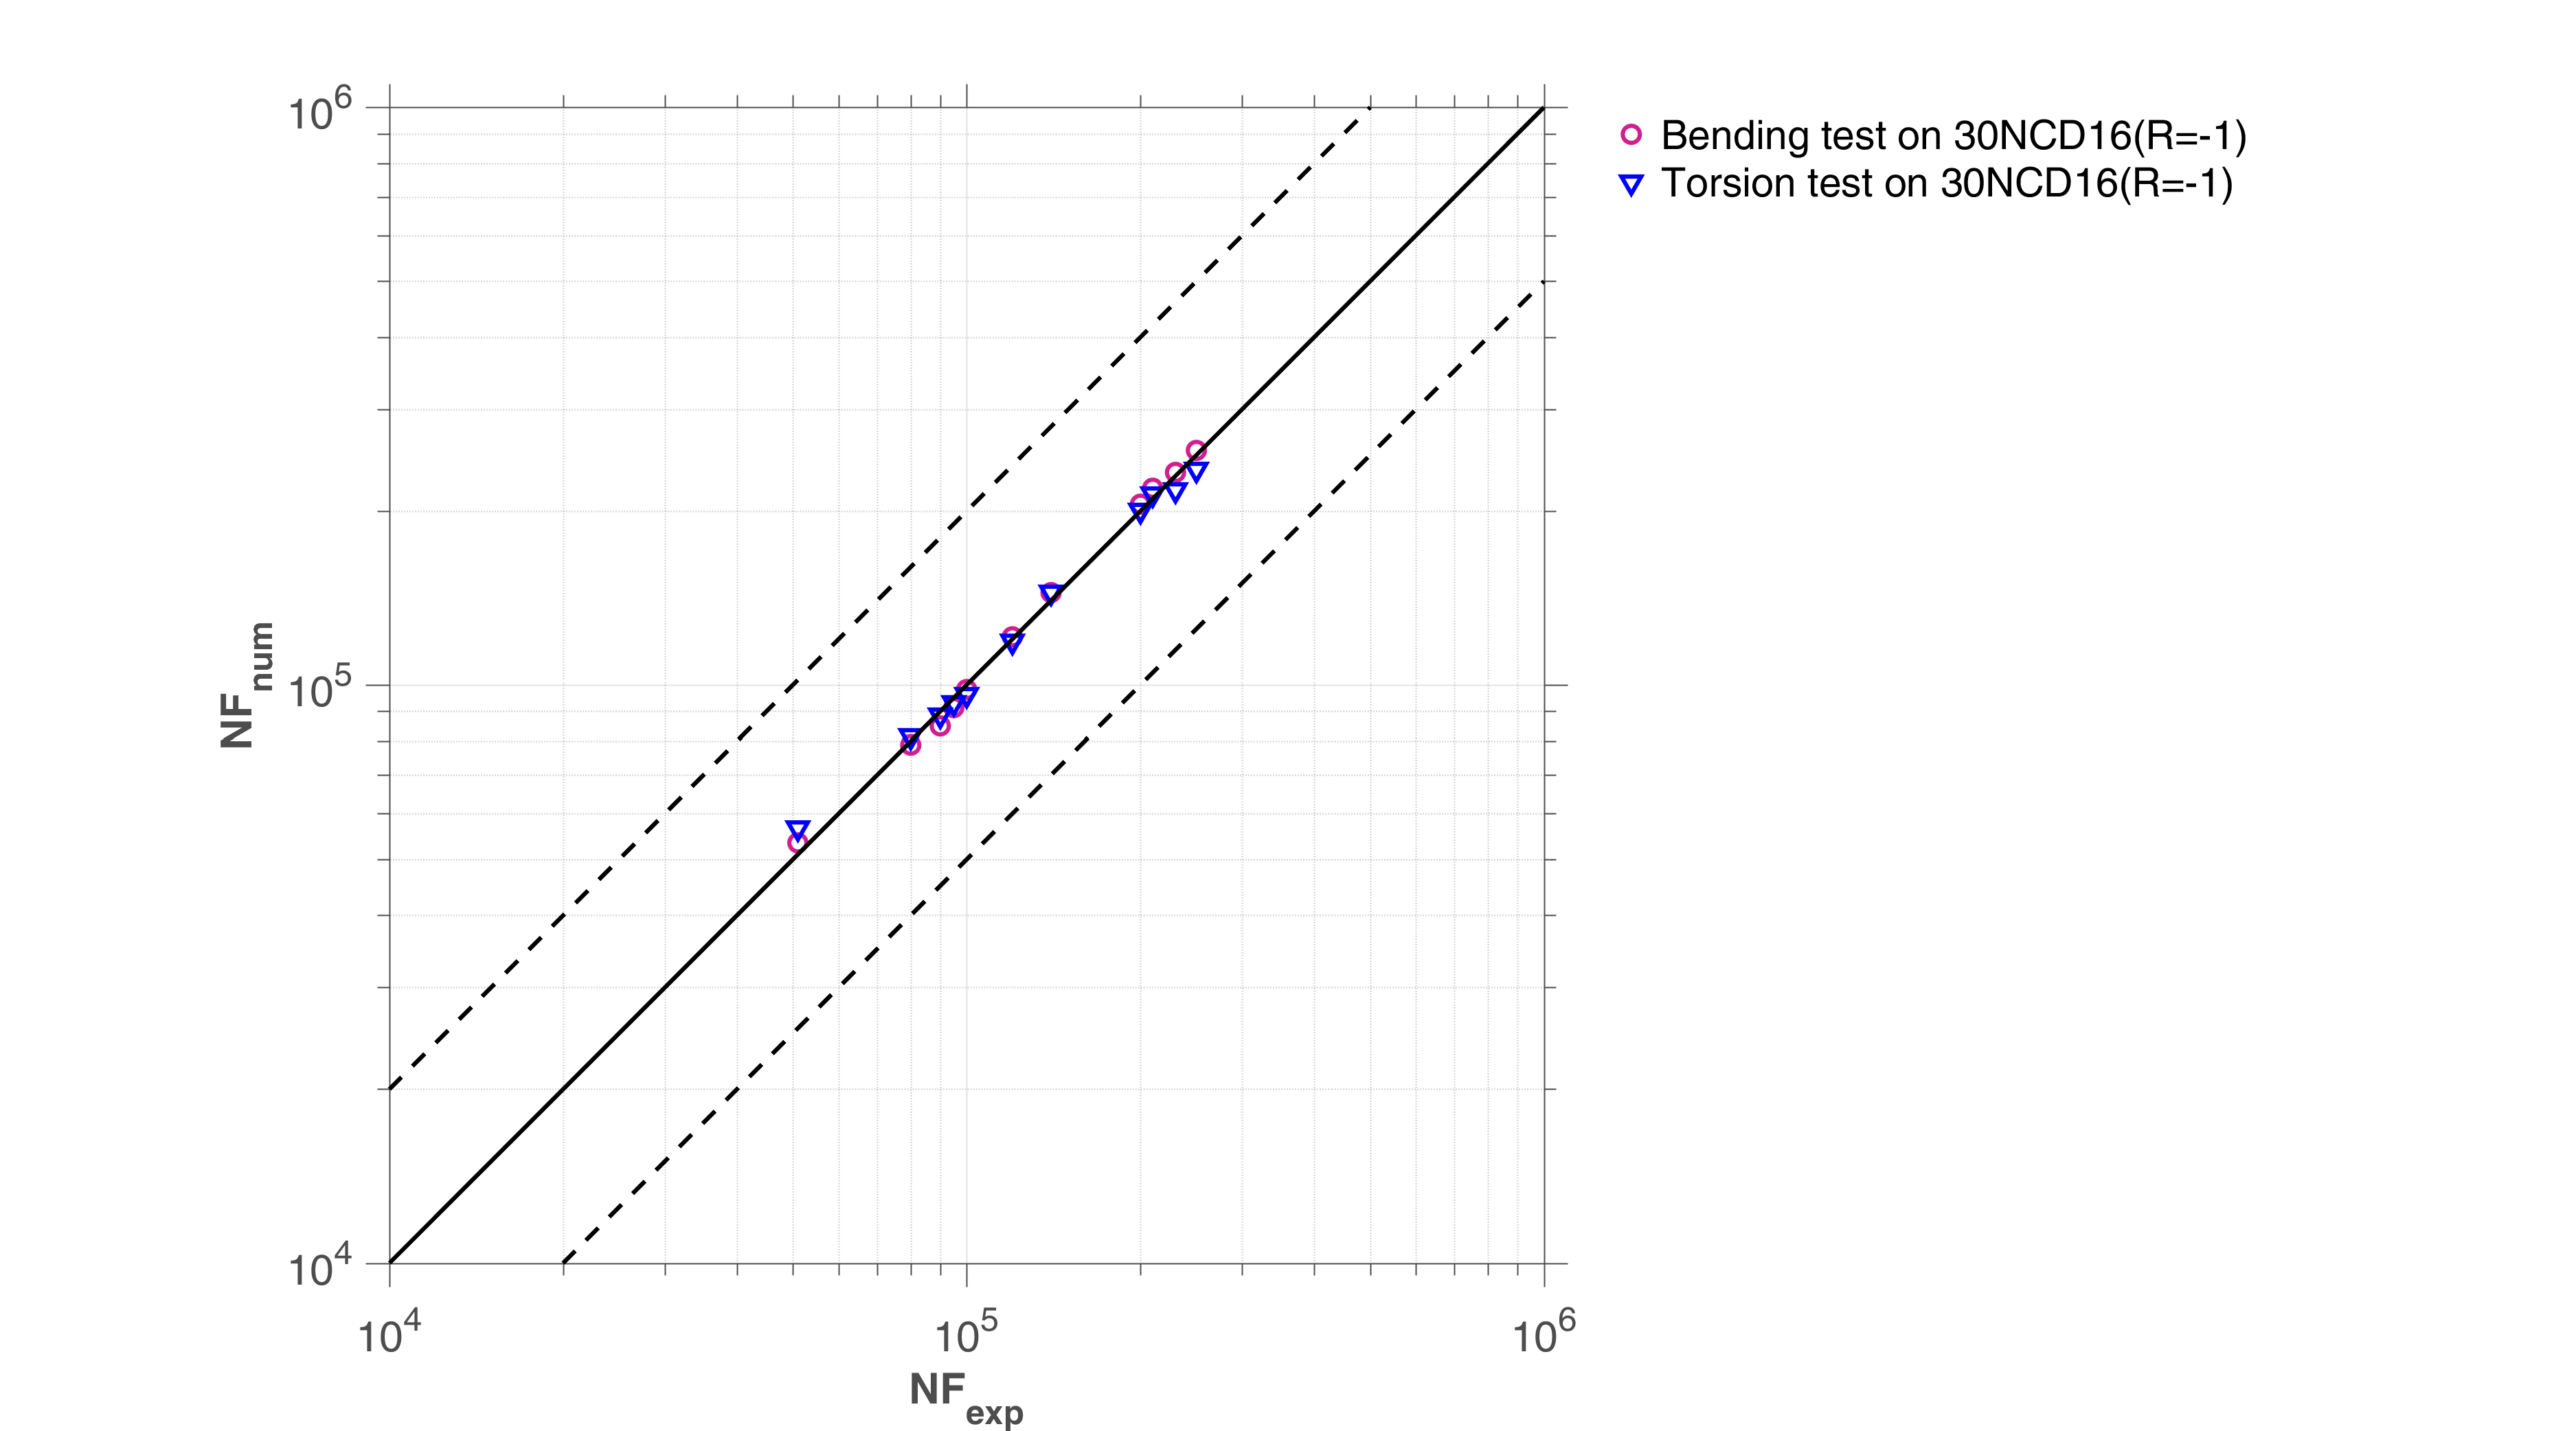
\includegraphics[width=\textwidth]{figures//bt1D_30NCD16_err1.png} 
	\caption{Bending and torsion tests on 30NCD16(R=-1)}
	\label{fig.bt1D30NCD16err1}
\end{figure}
\begin{figure}[!h]
	\centering
	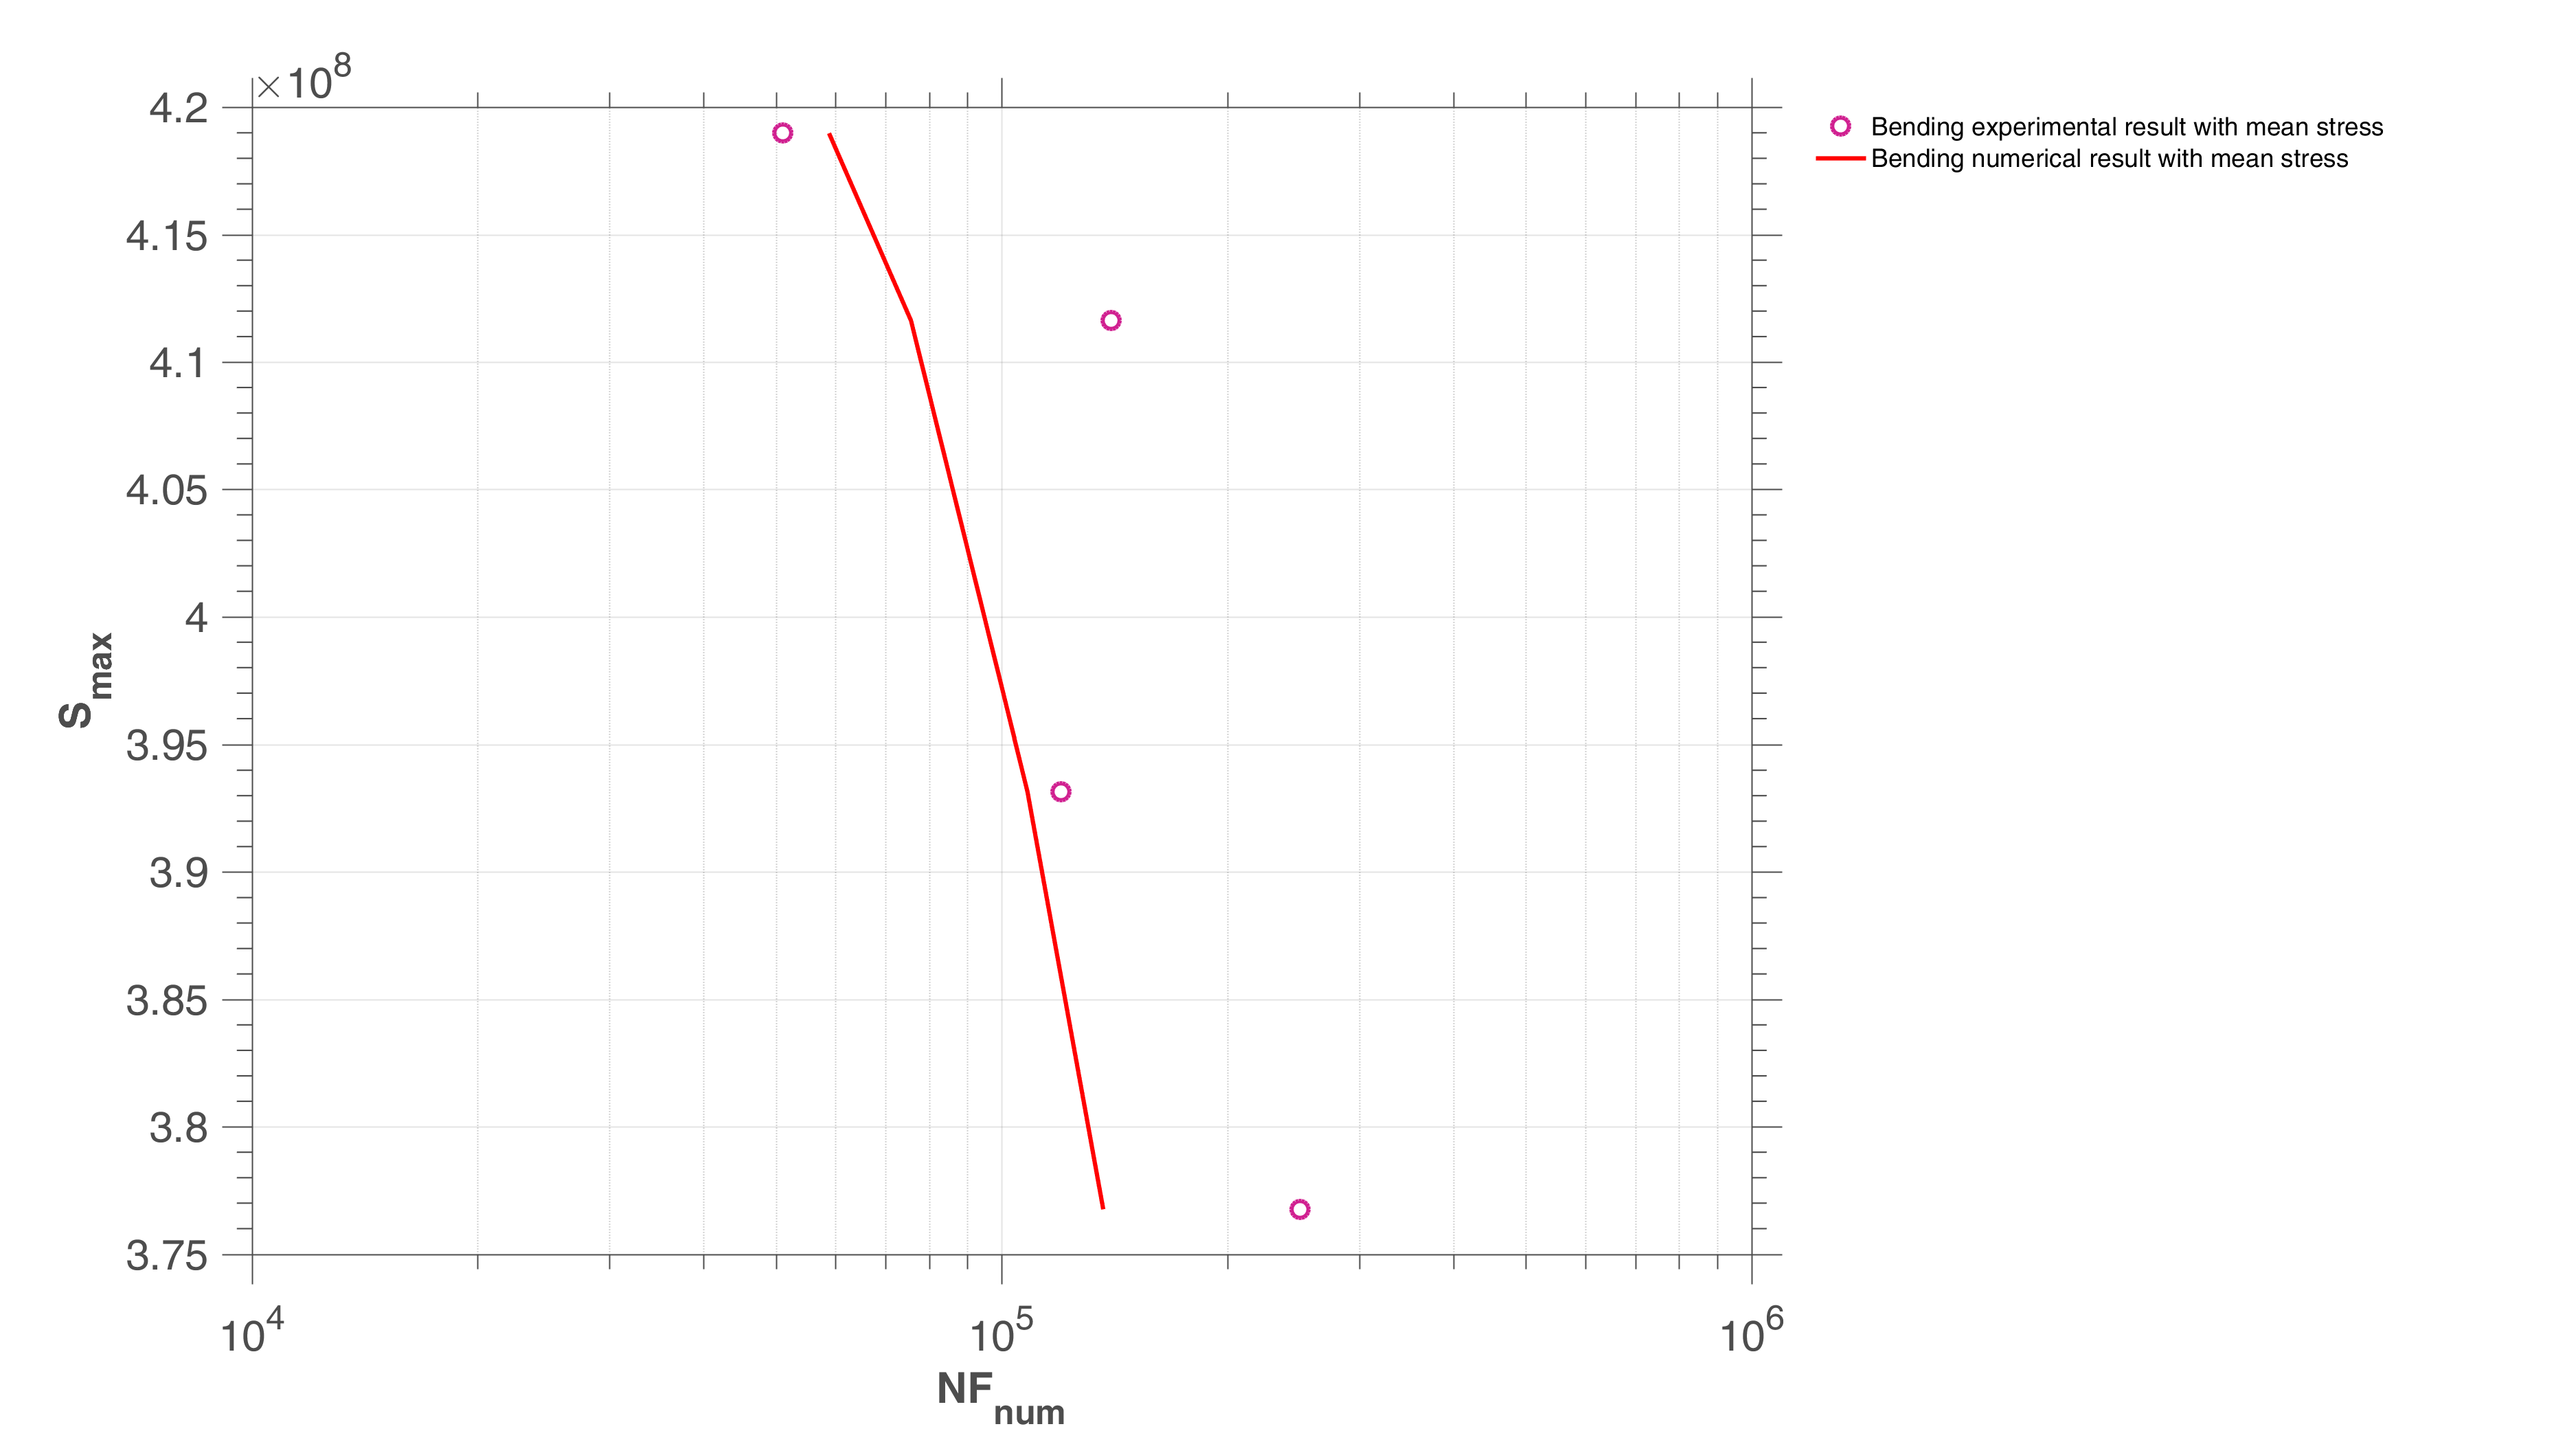
\includegraphics[width=\textwidth]{figures//b1D_m_30NCD16_sn.png} 
	\caption{Bending tests with mean stress on 30NCD16(R=-1)}
	\label{fig.b1Dm30NCD16sn}
\end{figure}

\begin{figure}[!h]
	\centering
	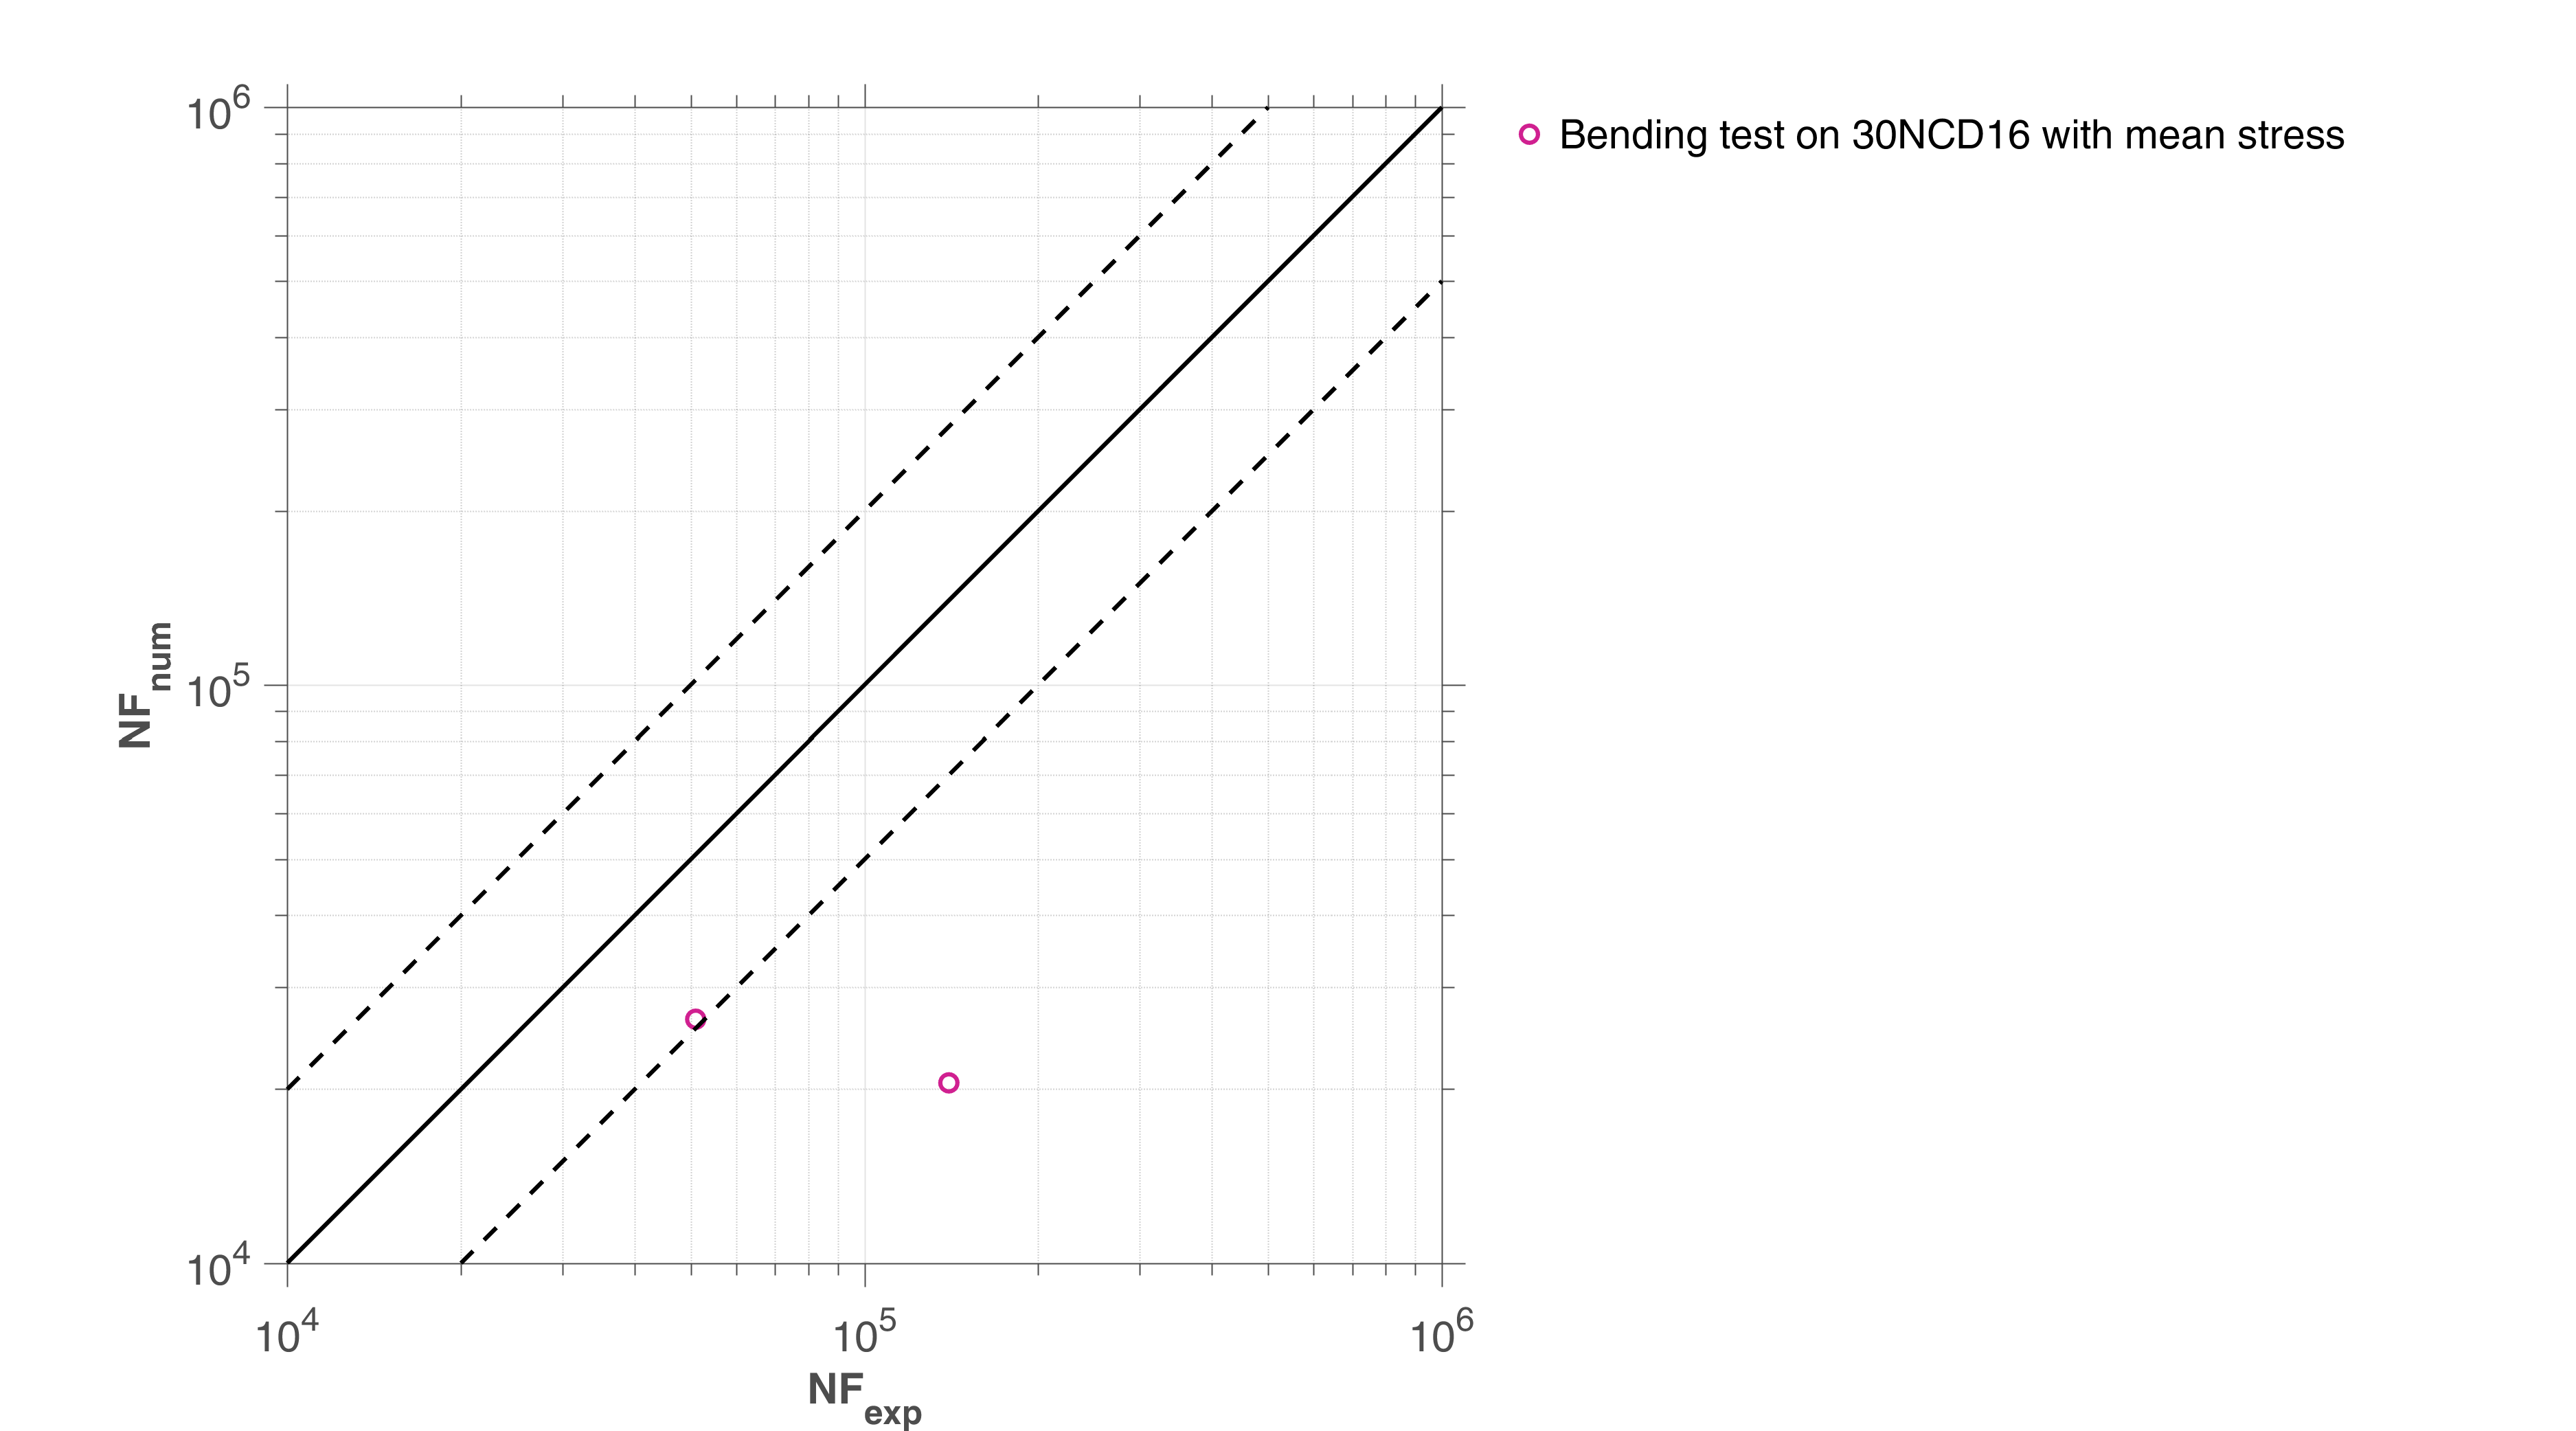
\includegraphics[width=\textwidth]{figures//b1D_m_30NCD16_err1.png} 
	\caption{Bending tests with mean stress on 30NCD16(R=-1)}
	\label{fig.b1Dm30NCD16err1}
\end{figure}

\begin{figure}[!h]
	\centering
	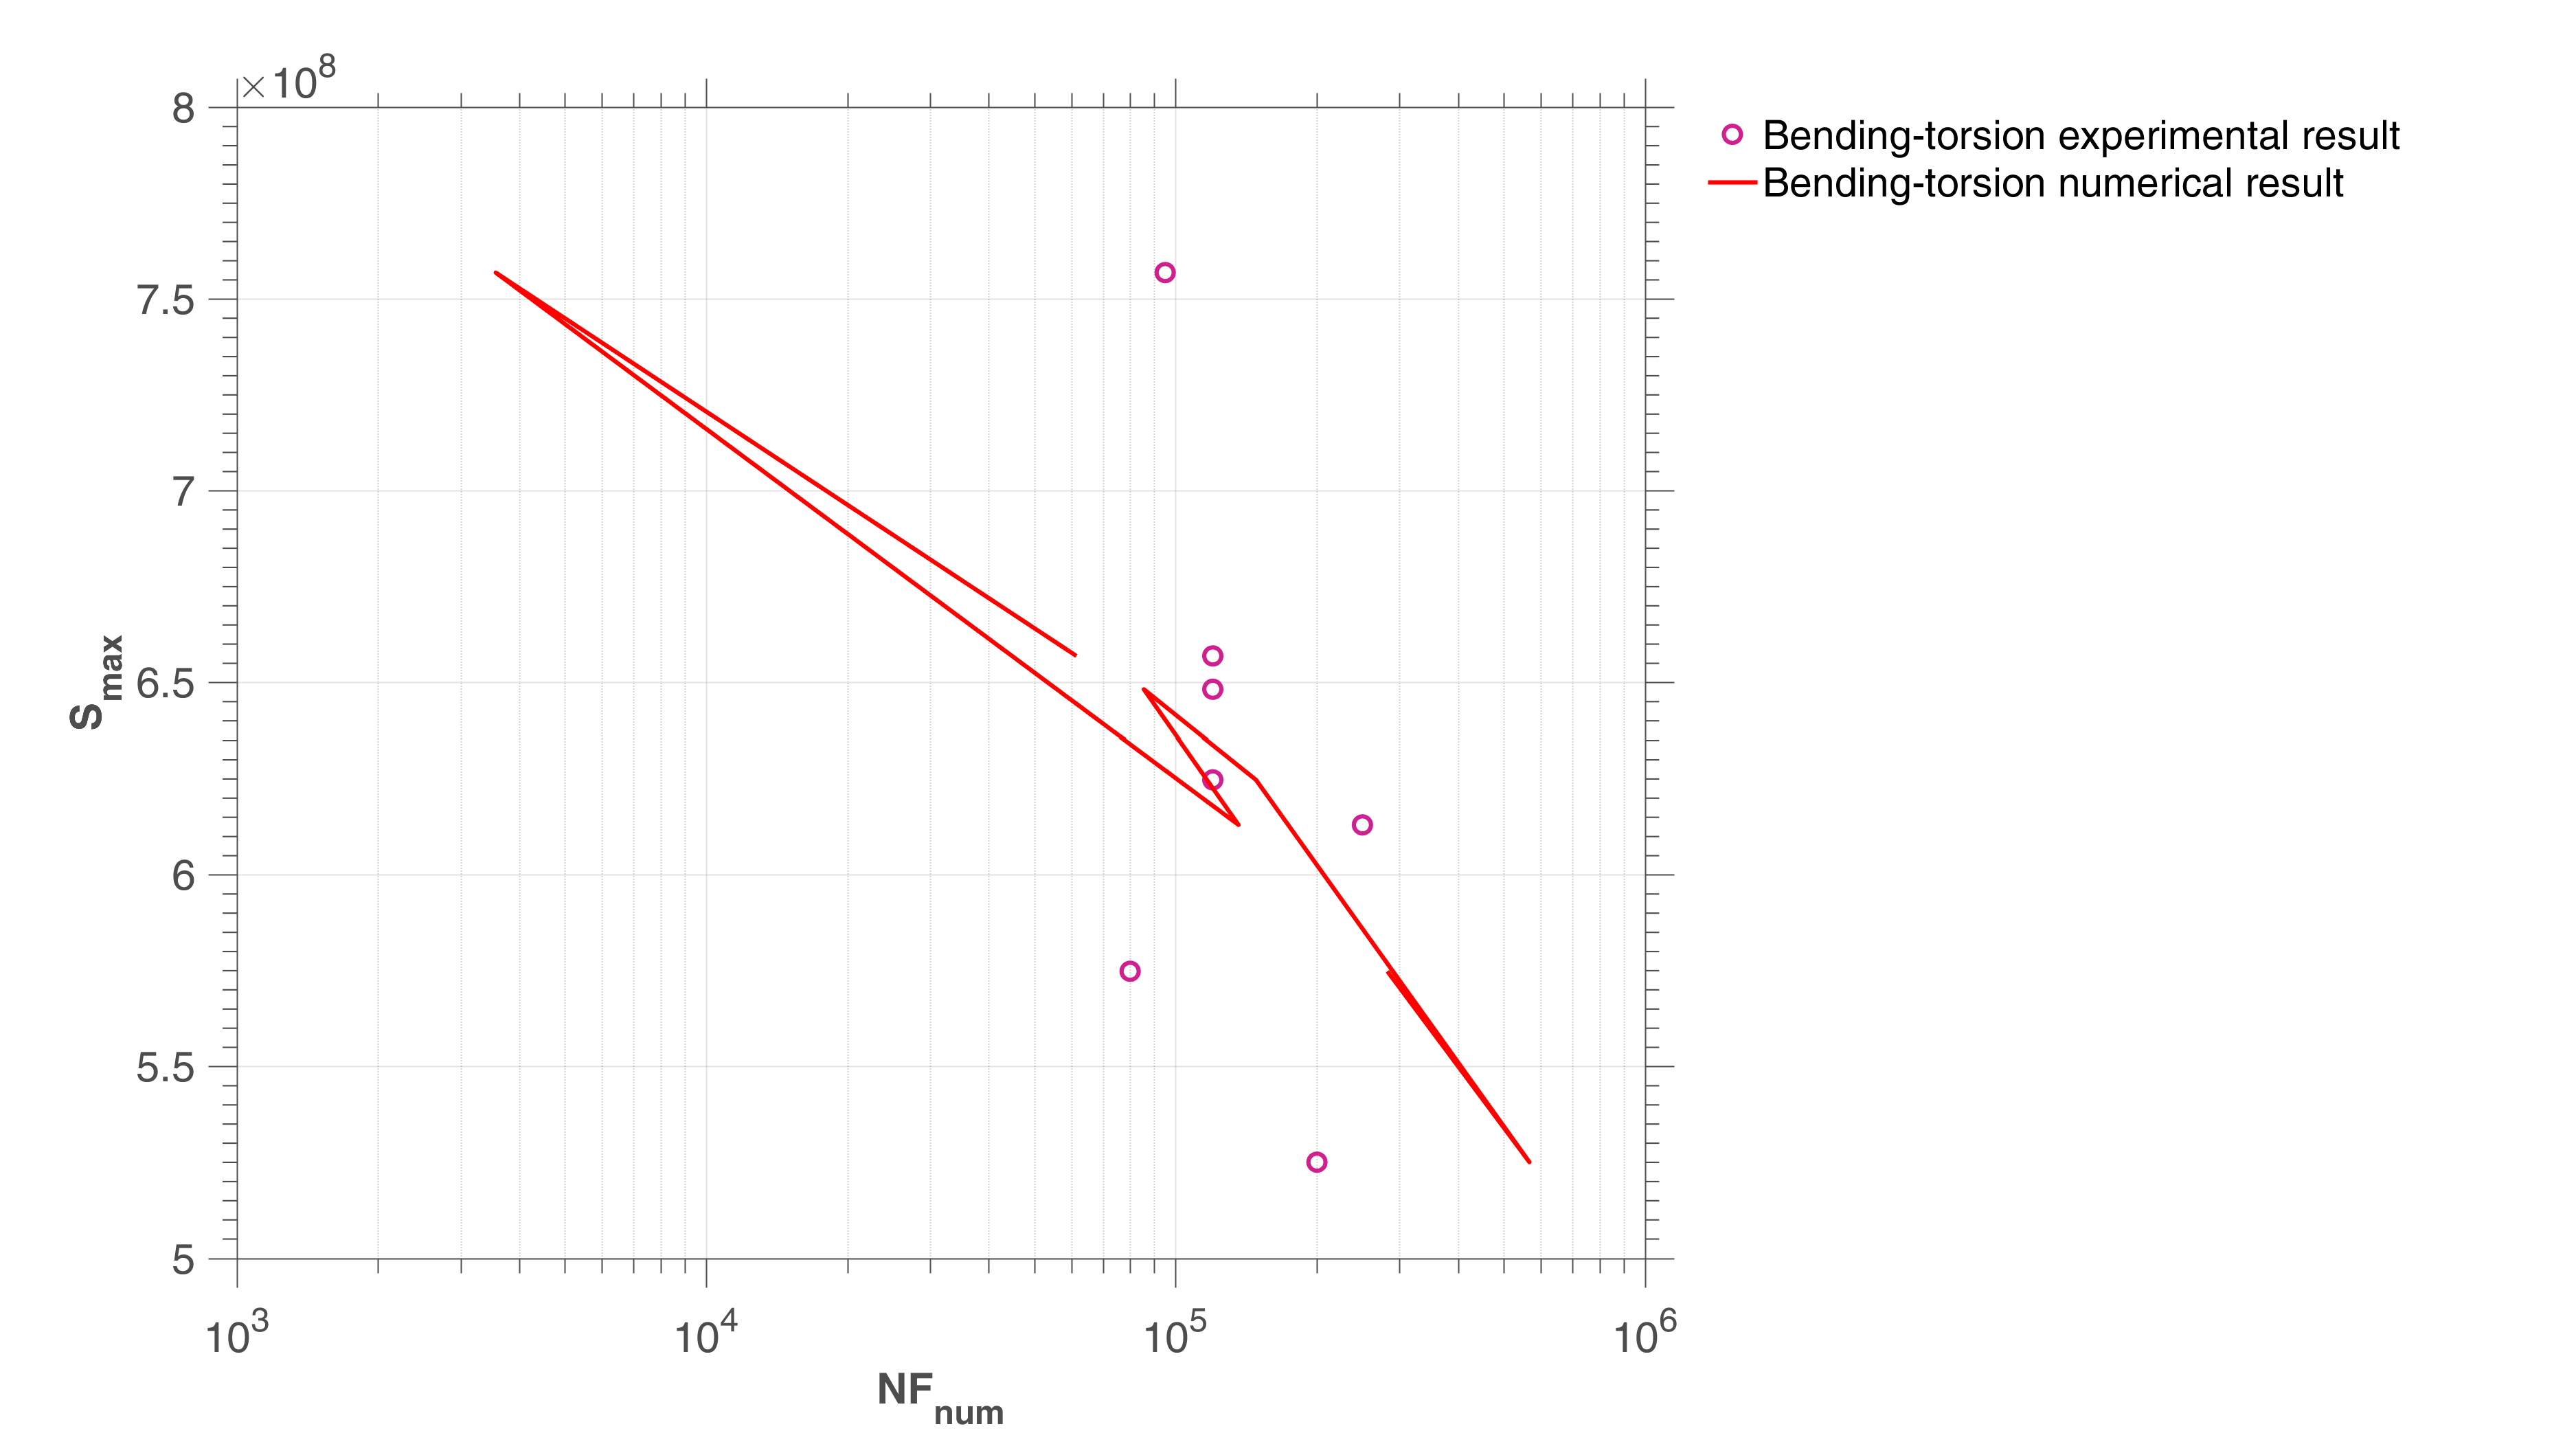
\includegraphics[width=\textwidth]{figures//bt2D_m_30NCD16_sn.png} 
	\caption{Bending-torsion tests with mean stress on 30NCD16}
	\label{fig.bt2Dm30NCD16sn}
\end{figure}
\begin{figure}[!h]
	\centering
	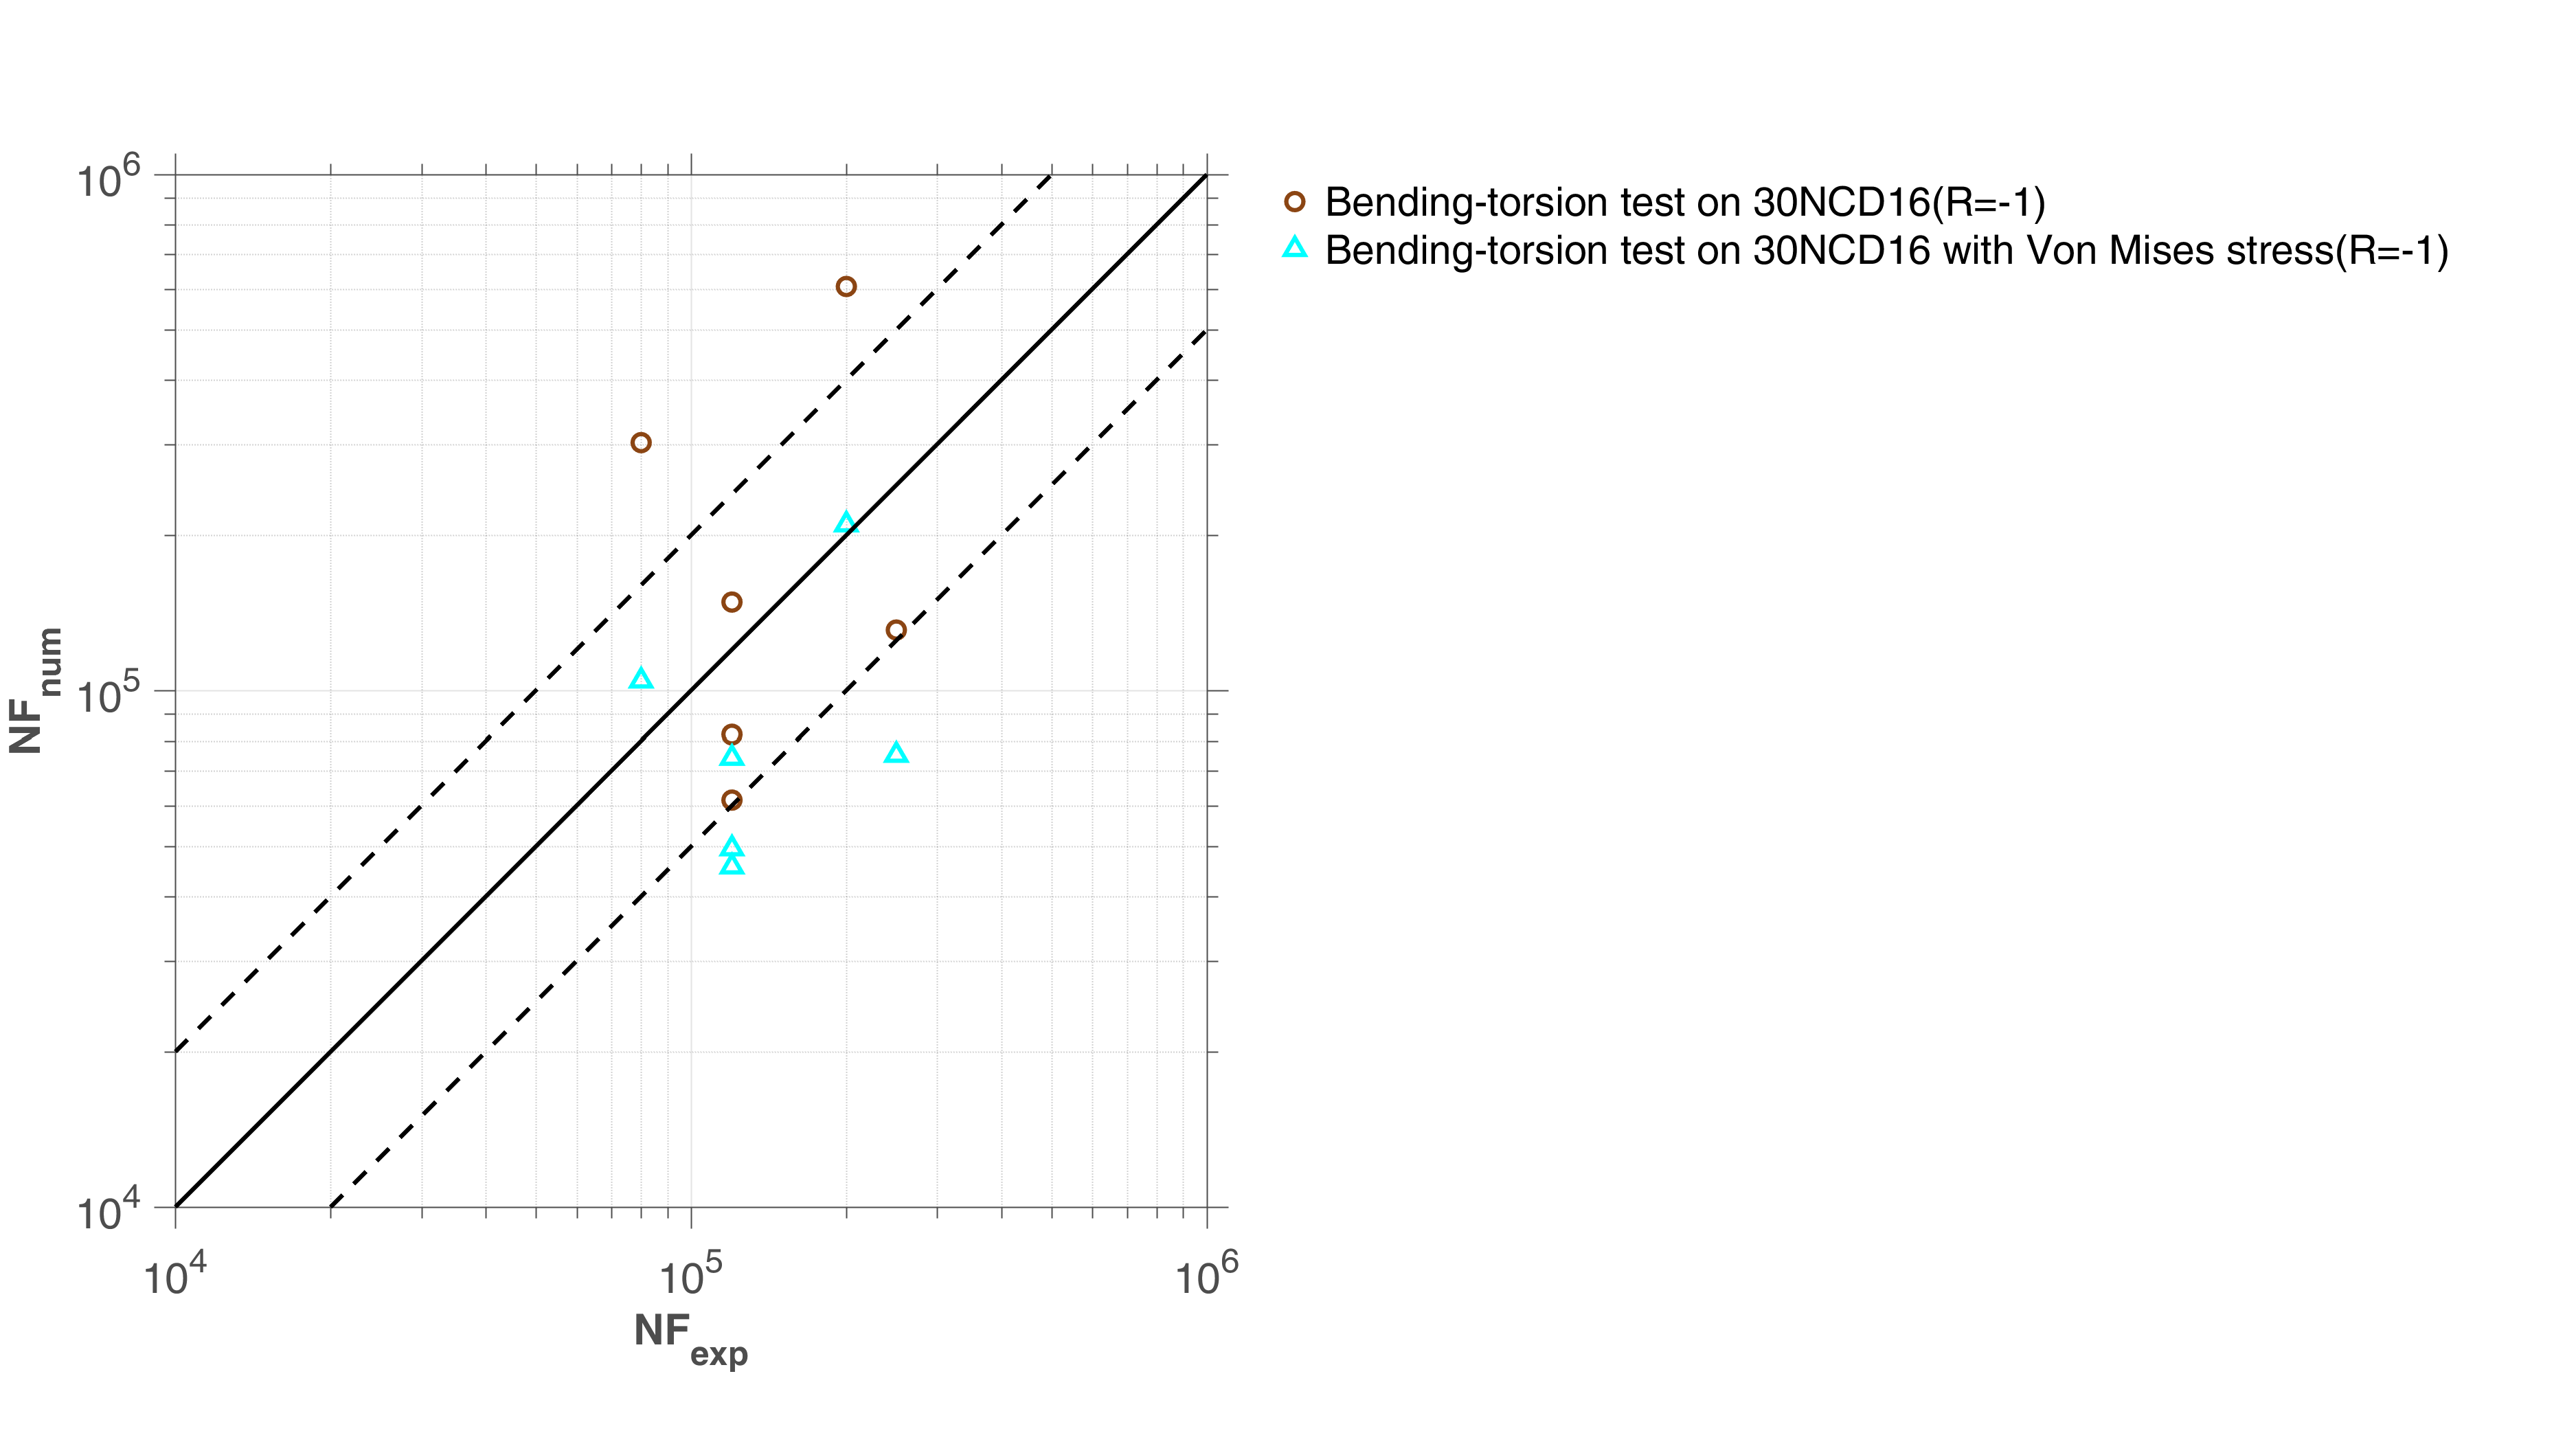
\includegraphics[width=\textwidth]{figures//bt2D_m_30NCD16_err1.png} 
	\caption{Bending-torsion tests with mean stress on 30NCD16}
	\label{fig.bt2Dm30NCD16err1}
\end{figure}


\clearpage
\subsection{Experimental validation of the model on SM45C steel}
\subsubsection{Presentation of steel SM45C}
This is a structural steel widespread use for the crankshafts and the structural components. The chemical composition and mechanical properties of this material is given in Table. \ref{SM45Cchem} and Table. \ref{SM45Cmec}.

\begin{table}[!h]
	\centering
	\begin{tabular}{|c|c|c|c|c|c|c|c|}
		\hline
		\textbf{C} & \textbf{Mn} & \textbf{P} & \textbf{S} & \textbf{Si} & \textbf{Ni} & \textbf{Cr} & \textbf{Cu} \\ \hline
		0.42       & 0.73        & 0.02       & 0.012      & 0.28        & 0.14        & 0.18        & 0.13        \\ \hline
	\end{tabular}
	\caption{Chemical composition of SM45C steel}
	\label{SM45Cchem}
\end{table}
\begin{table}[!h]
	\centering
	\begin{tabular}{|c|c|c|c|c|c|}
		\hline
		\textbf{\begin{tabular}[c]{@{}c@{}}$\sigma_{y}$\\ {[}MPa{]}\end{tabular}} & \textbf{\begin{tabular}[c]{@{}c@{}}$\sigma_{u}$\\ {[}MPa{]}\end{tabular}} & \textbf{\begin{tabular}[c]{@{}c@{}}E\\ {[}GPa{]}\end{tabular}} & \textbf{\begin{tabular}[c]{@{}c@{}}G\\ {[}GPa{]}\end{tabular}} & \textbf{$\nu$} & \textbf{A} \\ \hline
		638                                                                       & 824                                                                       & 213                                                            & 82.5                                                           & 0.29           & 22         \\ \hline
	\end{tabular}
	\caption{Mechanical and dynamic characteristics of SM45C steel}
	\label{SM45Cmec}
\end{table}

\begin{flushleft}
	E: Young's modulus,
	
	G: Shear modulus,
	
	$\nu$: Poisson ratio,
	
	A:	Elongation at break.
\end{flushleft}
\newpage
\subsubsection{Fatigue tests performed by Dubar on steel SM45C}
Preliminary fatigue tests in purely alternating torsion and purely alternating flexion were performed by Lee \cite{lee2013out}. These two types of tests were carried out with test pieces of the same geometric shape. In addition, the author had performed moderate stress bending fatigue tests to study its effect on the lifetime of SM45C steel. All uniaxial fatigue tests performed by Lee \cite{lee2013out} are illustrated in \figref{fig.SM45CSN}. This figure shows a reduction in bending life of SM45C steel in the presence of a positive mean stress. Crack initiation was detected when the stiffness of the specimen or specimen used was reduced by 10\%.
\begin{figure}[!h]
	\centering
	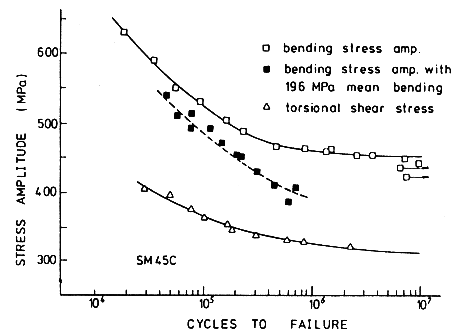
\includegraphics[width=0.8\textwidth]{figures//SM45C_SN.png} 
	\caption{Fatigue curves made on SM45C steel by Lee \cite{lee2013out}}
	\label{fig.SM45CSN}
\end{figure}


Preliminary fatigue tests were carried out under fully reversed bending and torsion separately.
\begin{table}[!h]
	\centering
	\begin{tabular}{|c|c|c|c|}
		\hline
		\begin{tabular}[c]{@{}c@{}}Bending Tests\\ (R=-1)\end{tabular}& \begin{tabular}[c]{@{}c@{}}N\\ {[}Cycles{]}\end{tabular} & \begin{tabular}[c]{@{}c@{}}$\sigma_{x,a}$\\ {[}MPa{]}\end{tabular} & \begin{tabular}[c]{@{}c@{}}$\sigma_{x,m}$\\ {[}MPa{]}\end{tabular}\\ \hline
		1                                                                       & 1.9E4                                                             & 620                                                                    & 0                            \\ \hline
		2                                                                       & 3.6E4                                                             & 590                                                                    & 0                              \\ \hline
		3                                                                       & 5.8E4                                                             & 552                                                                     & 0                             \\ \hline
		4                                                                       & 9E4                                                               & 535                                                                     & 0                             \\ \hline
		5                                                                       & 1.7E5                                                             & 505                                                                       & 0                           \\ \hline
		6                                                                       & 2.2E5                                                             & 490                                                                        & 0                          \\ \hline
		7                                                                       & 4.4E5                                                             & 470                                                                         & 0                         \\ \hline
		8                                                                       & 8E5                                                               & 465                                                                         & 0                         \\ \hline
		9                                                                       & 1.4E6                                                             & 462                                                                         & 0                         \\ \hline
		10                                                                      & 1.5E6                                                             & 465                                                                         & 0                         \\ \hline
		11                                                                      & 2.4E6                                                             & 460                                                                         & 0                         \\ \hline
		12                                                                      & 3.3E6                                                             & 460                                                                         & 0                         \\ \hline
		13                                                                      & 6E6                                                               & 440                                                                          & 0                        \\ \hline
		14                                                                      & 6.6E6                                                             & 458                                                                          & 0                        \\ \hline
		15                                                                      & 7E6                                                               & 430                                                                          & 0                        \\ \hline
		16                                                                      & 9E6                                                               & 448                                                                          & 0                        \\ \hline \hline
		17                                                                      & 4.5E4                                                               & 540                                                                          & 196                        \\ \hline
		18                                                                      & 5.4E4                                                               & 515                                                                          & 196                         \\ \hline
		19                                                                      & 7E4                                                               & 520                                                                          & 196                         \\ \hline
		20                                                                      & 7.1E4                                                               & 485                                                                          & 196                        \\ \hline
		21                                                                      & 1.1E5                                                               & 485                                                                          & 196                       \\ \hline
		22                                                                      & 1.5E5                                                               & 475                                                                          & 196                       \\ \hline
		23                                                                      & 2E5                                                               & 460                                                                          & 196                      \\ \hline
		24                                                                      & 2.1E5                                                               & 455                                                                          & 196                        \\ \hline
		25                                                                      & 3E5                                                               & 435                                                                          & 196                       \\ \hline
		26                                                                      & 4.3E5                                                              & 415                                                                          & 196                         \\ \hline
		27                                                                      & 6.9E5                                                               & 410                                                                          & 196                         \\ \hline
		28                                                                      & 5.8E5                                                               & 390                                                                          & 196                        \\ \hline
	\end{tabular}
	\caption{SM45C steel fully reversed bending tests(extracted from  \cite{lee2013out})}
	\label{SM45Cbendingr1}
\end{table}

\begin{table}[!h]
	\centering
	\begin{tabular}{|c|c|c|}
		\hline
		\begin{tabular}[c]{@{}c@{}}Torsion Tests\\ (R=-1)\end{tabular} & \begin{tabular}[c]{@{}c@{}}N\\ {[}Cycles{]}\end{tabular} & \begin{tabular}[c]{@{}c@{}}$\tau_{xy,a}$\\ {[}MPa{]}\end{tabular} \\ \hline
		1                                                                       & 2.9E4                                                             & 405                                                                                                \\ \hline
		2                                                                       & 5E4                                                               & 399                                                                                                \\ \hline
		3                                                                       & 7.8E4                                                             & 380                                                                                                \\ \hline
		4                                                                       & 1E5                                                               & 365                                                                                                \\ \hline
		5                                                                       & 1.8E5                                                             & 355                                                                                                \\ \hline
		6                                                                       & 1.9E5                                                             & 349                                                                                                \\ \hline
		7                                                                       & 3E5                                                               & 340                                                                                                \\ \hline
		8                                                                       & 5.8E5                                                             & 335                                                                                                \\ \hline
		9                                                                       & 8.2E5                                                             & 333                                                                                                \\ \hline
		10                                                                      & 2.25E6                                                            & 325                                                                                                \\ \hline
	\end{tabular}
	\caption{SM45 steel fully reversed torsion tests(extracted from  \cite{lee2013out})}
	\label{SM45CtorsionR1}
\end{table}



\begin{table}[!h]
	\centering
	\begin{tabularx}{\textwidth}{XXXXX}
		\hline
		\textbf{Group}               & \multicolumn{1}{l}{\textbf{\begin{tabular}[l]{@{}c@{}}N\\ {[}Cycles{]}\end{tabular}}} & \multicolumn{1}{l}{\textbf{\begin{tabular}[l]{@{}c@{}}$\tau_a$\\ {[}MPa{]}\end{tabular}}} & \multicolumn{1}{l}{\textbf{\begin{tabular}[l]{@{}c@{}}$\sigma_a$\\ {[}MPa{]}\end{tabular}}} & \multicolumn{1}{l}{\textbf{\begin{tabular}[l]{@{}c@{}}$\sigma_m$\\ {[}MPa{]}\end{tabular}}} \\ \hline
		\multirow{10}{*}{\textbf{A}} & 29.9E3                                                                                & 282                                                                                       & 449                                                                                         & 0                                                                                           \\
		& 35.7E3                                                                                & 334                                                                                       & 354                                                                                         & 0                                                                                           \\
		& 50E3                                                                                  & 223                                                                                       & 485                                                                                         & 0                                                                                           \\
		& 73.8E3                                                                                & 309                                                                                       & 357                                                                                         & 0                                                                                           \\
		& 106E3                                                                                 & 217                                                                                       & 449                                                                                         & 0                                                                                           \\
		& 106E3                                                                                 & 285                                                                                       & 370                                                                                         & 0                                                                                           \\
		& 112E3                                                                                 & 199                                                                                       & 449                                                                                         & 0                                                                                           \\
		& 131E3                                                                                 & 194                                                                                       & 457                                                                                         & 0                                                                                           \\
		& 333E3                                                                                 & 252                                                                                       & 354                                                                                         & 0                                                                                           \\
		& 431E3                                                                                 & 154                                                                                       & 437                                                                                         & 0                                                                                           \\ \hline
		\multirow{10}{*}{\textbf{B}} & 53E3                                                                                  & 215                                                                                       & 441                                                                                         & 196                                                                                         \\
		& 59.2E3                                                                                & 309                                                                                       & 286                                                                                         & 196                                                                                         \\
		& 70.1E3                                                                                & 155                                                                                       & 464                                                                                         & 196                                                                                         \\
		& 86.3E3                                                                                & 136                                                                                       & 473                                                                                         & 196                                                                                         \\
		& 89.9E3                                                                                & 334                                                                                       & 173                                                                                         & 196                                                                                         \\
		& 92.1E3                                                                                & 209                                                                                       & 403                                                                                         & 196                                                                                         \\
		& 102E3                                                                                 & 177                                                                                       & 437                                                                                         & 196                                                                                         \\
		& 135E3                                                                                 & 321                                                                                       & 167                                                                                         & 196                                                                                         \\
		& 351E3                                                                                 & 179                                                                                       & 357                                                                                         & 196                                                                                         \\
		& 394E3                                                                                 & 274                                                                                       & 182                                                                                         & 196                                                                                         \\ \hline
	\end{tabularx}
	\caption{With and without mean bending stress on out-of-phase($90^\circ$) fatigue of SM45C steel \cite{lee2013out}}
	\label{meanSM45C}
\end{table}

In the case of multiaxial bending-torsion block tests(Table. \ref{meanSM45C}), we could alternatively adopt Von Mises stress as the value of $S_{max}$:
\begin{equation}
S_{max}=\sigma_{von}=\sqrt{\frac{1}{2}\left[ (\sigma_{xx}-\sigma_{yy})^2+(\sigma_{yy}-\sigma_{zz})^2+(\sigma_{zz}-\sigma_{xx})^2\right]+3(\tau_{xy}^2+\tau_{yz}^2+\tau_{zx}^2) }
\label{von}
\end{equation}

\newpage
\subsubsection{Identification of model parameters for steel SM45C}

We use the Von Mises yield strength combining the bending and torsion yield limits as $\sigma_y$. The fitted curve using experimental data in Table. \ref{meanSM45C} and data with mean stress effect is shown in \figref{fig.sm45c2Dmean}.
The tests on SM45C steel have illustrated that the mean bending stress has an influence on both uniaxial and multiaxial fatigue life. 

Although the uniaxial experimental data we extracted from Lee's curve \cite{lee2013out} of SM45C steel are slightly dispersed, we can find our model quite satisfactory in the case of SM45C steel. As for multiaxial 90 degree out of phase, fully reversed bending-torsion fatigue tests, our model is able to evaluate the cycles to failure.

\begin{table}[!h]
	\centering
	\begin{tabular}{|c|c|c|}
		\hline
		\textbf{$\beta$} & \textbf{$\lambda$}  & \textbf{$W_0/a$}  \\ \hline
	 3.8        & 0.55            & 1000 GPa       \\ \hline
	\end{tabular}
	\caption{Parameter identification of 30NCD16 steel}
	\label{sm45cpara}
\end{table}

\begin{figure}[!h]
	\centering
	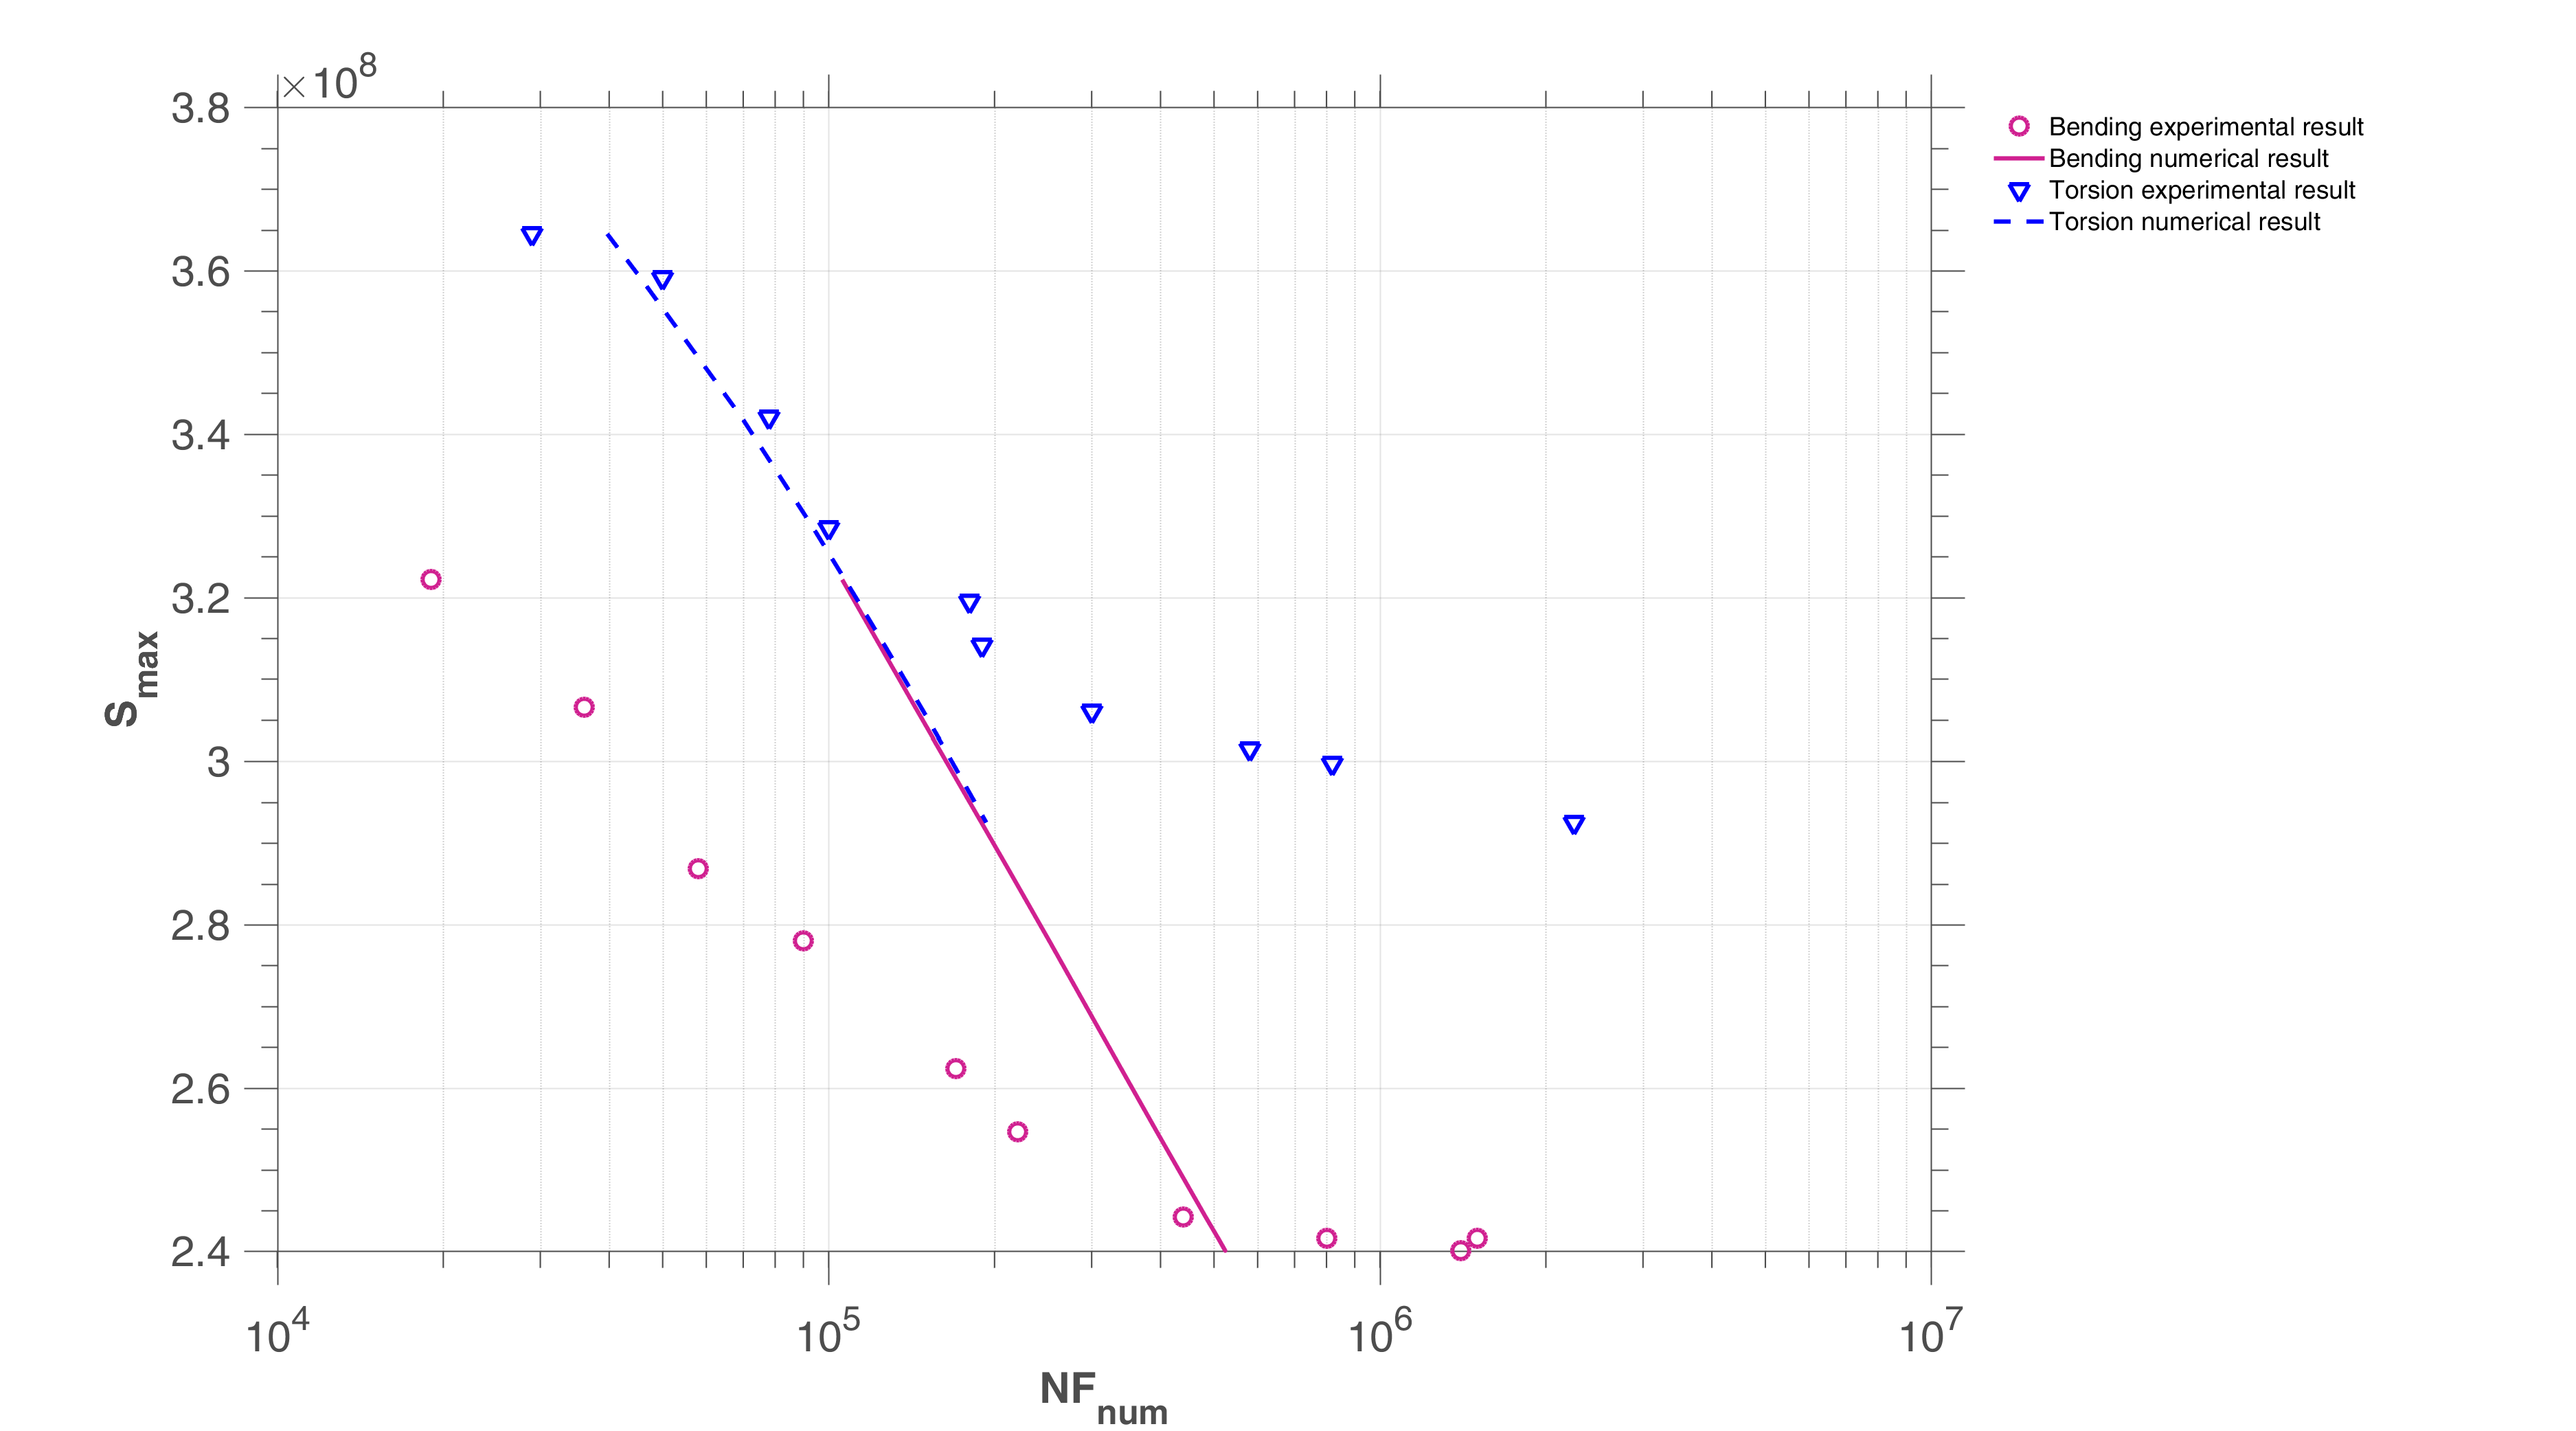
\includegraphics[width=\textwidth]{figures//bt1D_SM45C_sn.png} 
	\caption{Bending and torsion test on SM45C steel(R=-1)}
	\label{fig.bt1DSM45Csn}
\end{figure}
\begin{figure}[!h]
	\centering
	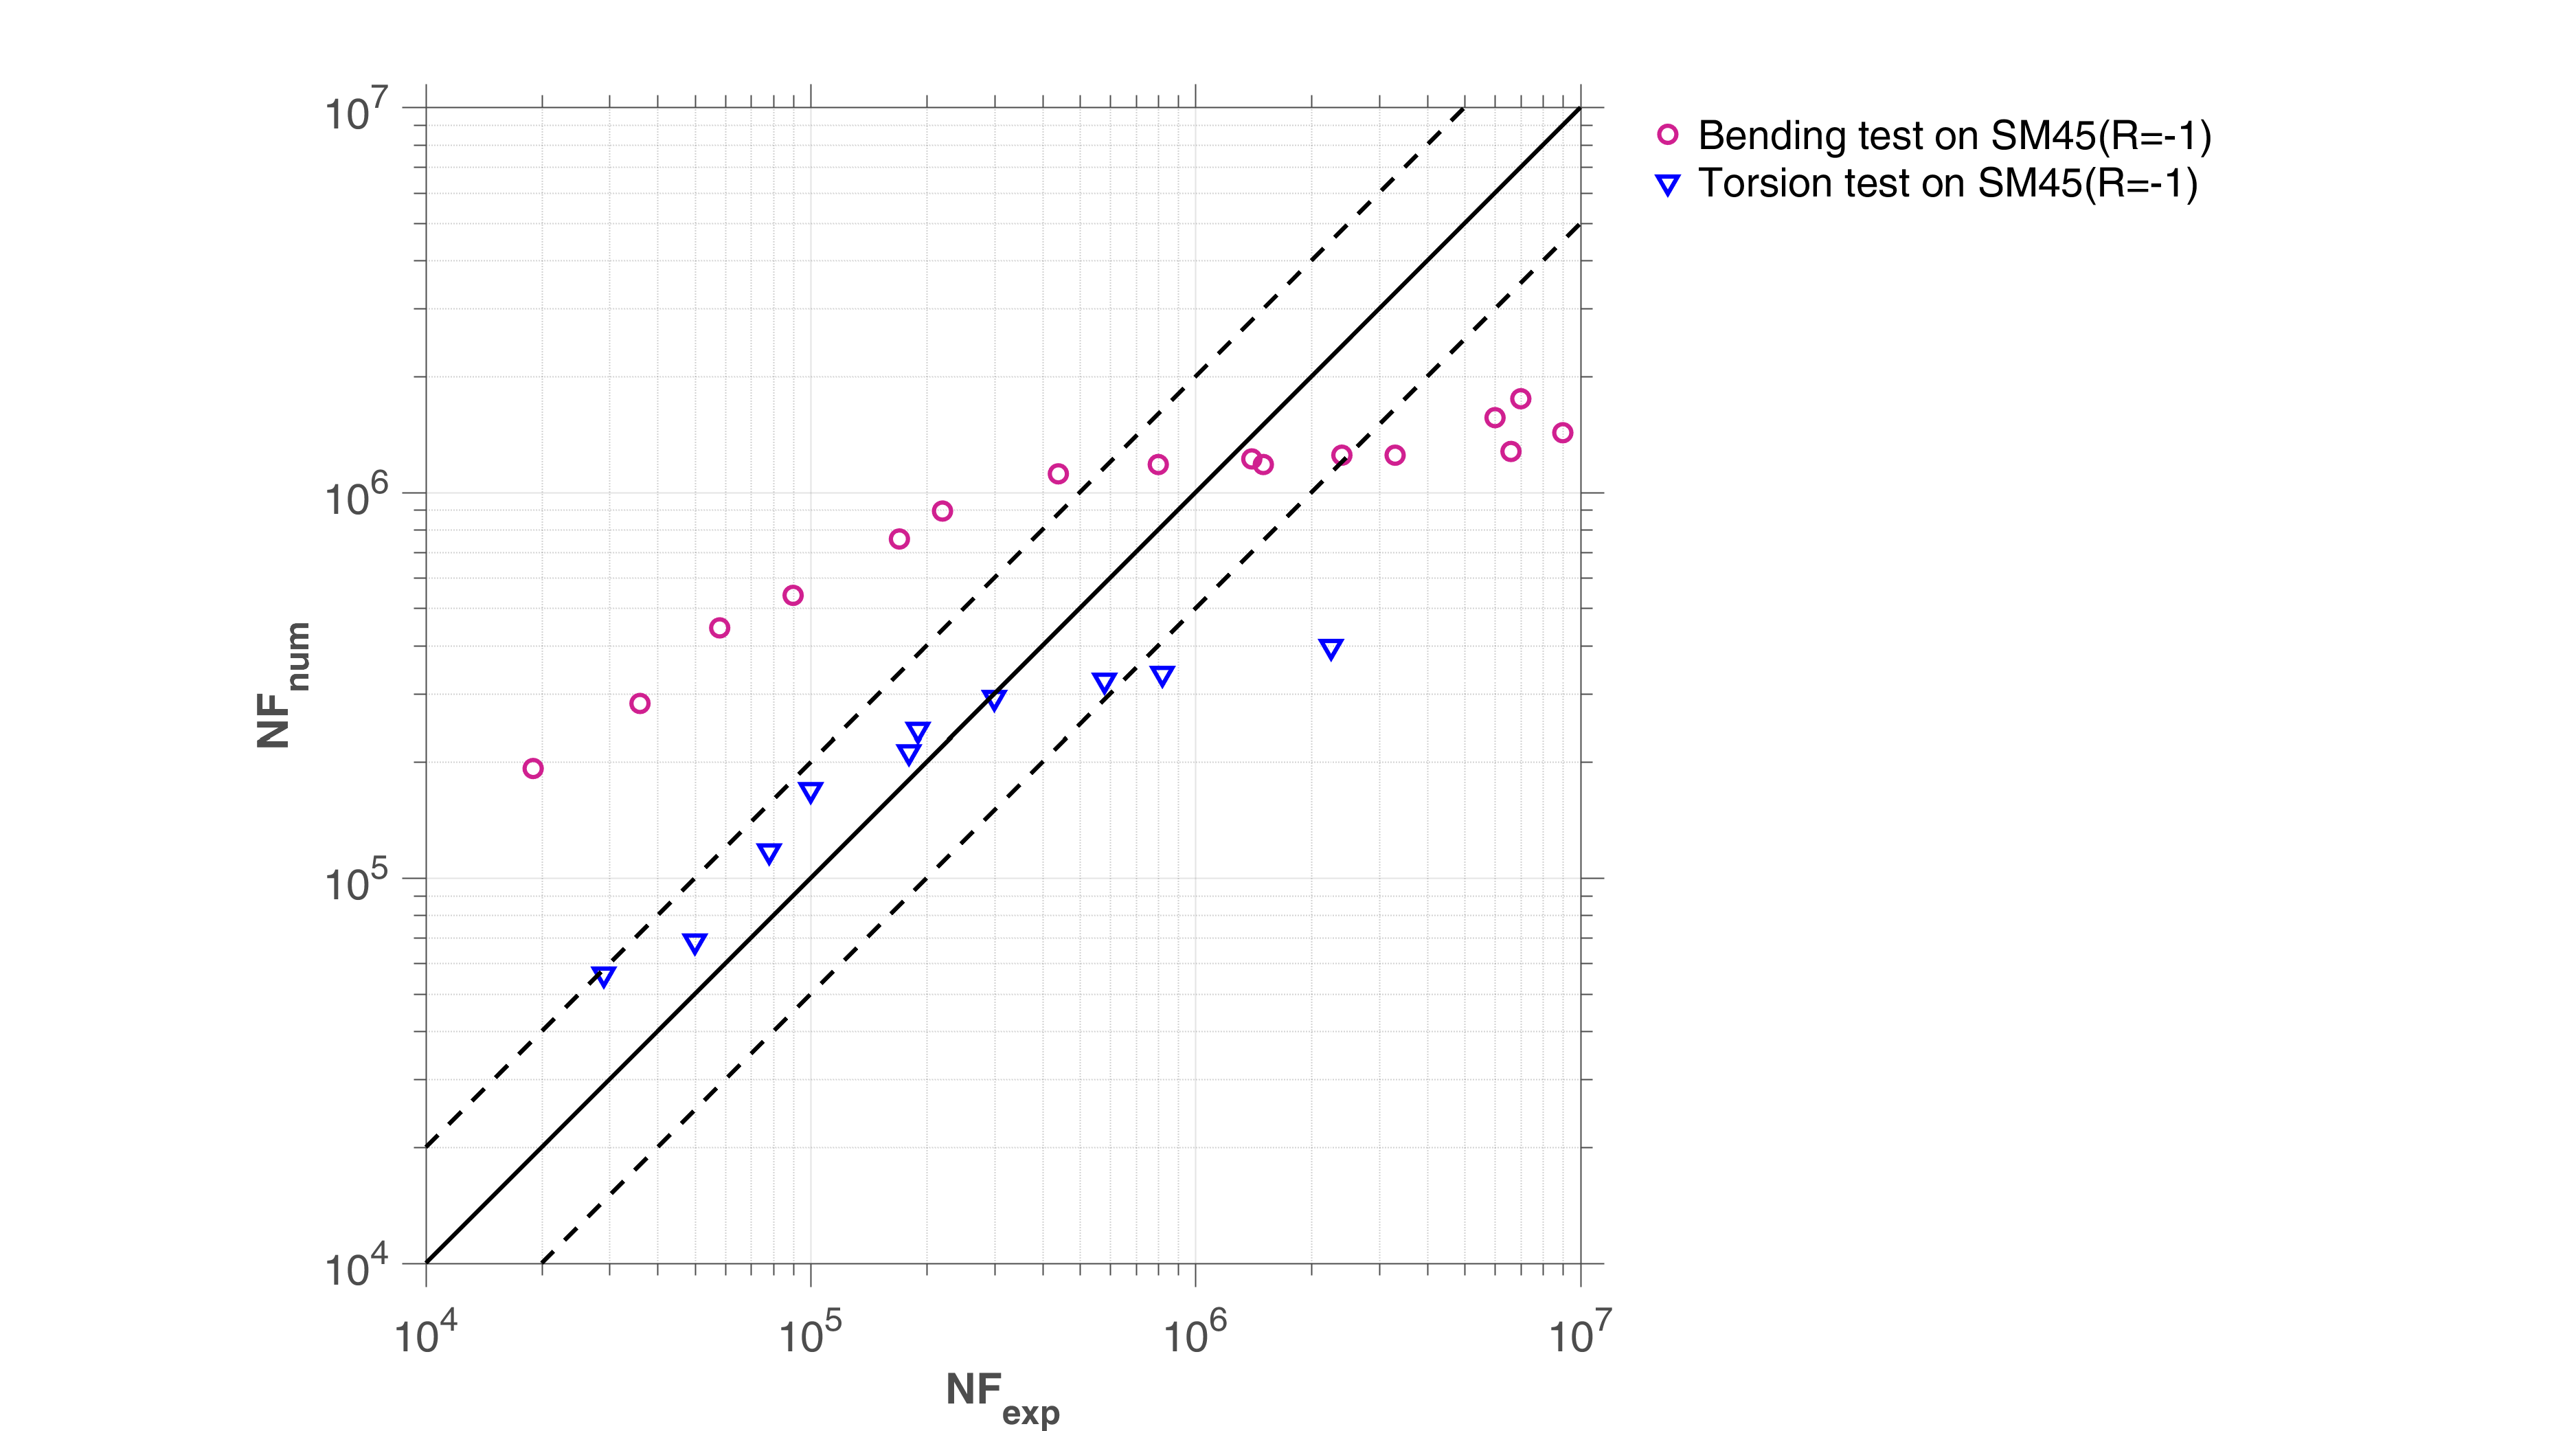
\includegraphics[width=\textwidth]{figures//bt1D_SM45C_err1.png} 
	\caption{Bending and torsion test on SM45C steel(R=-1)}
	\label{fig.bt1DSM45Cerr1}
\end{figure}
\begin{figure}[!h]
	\centering
	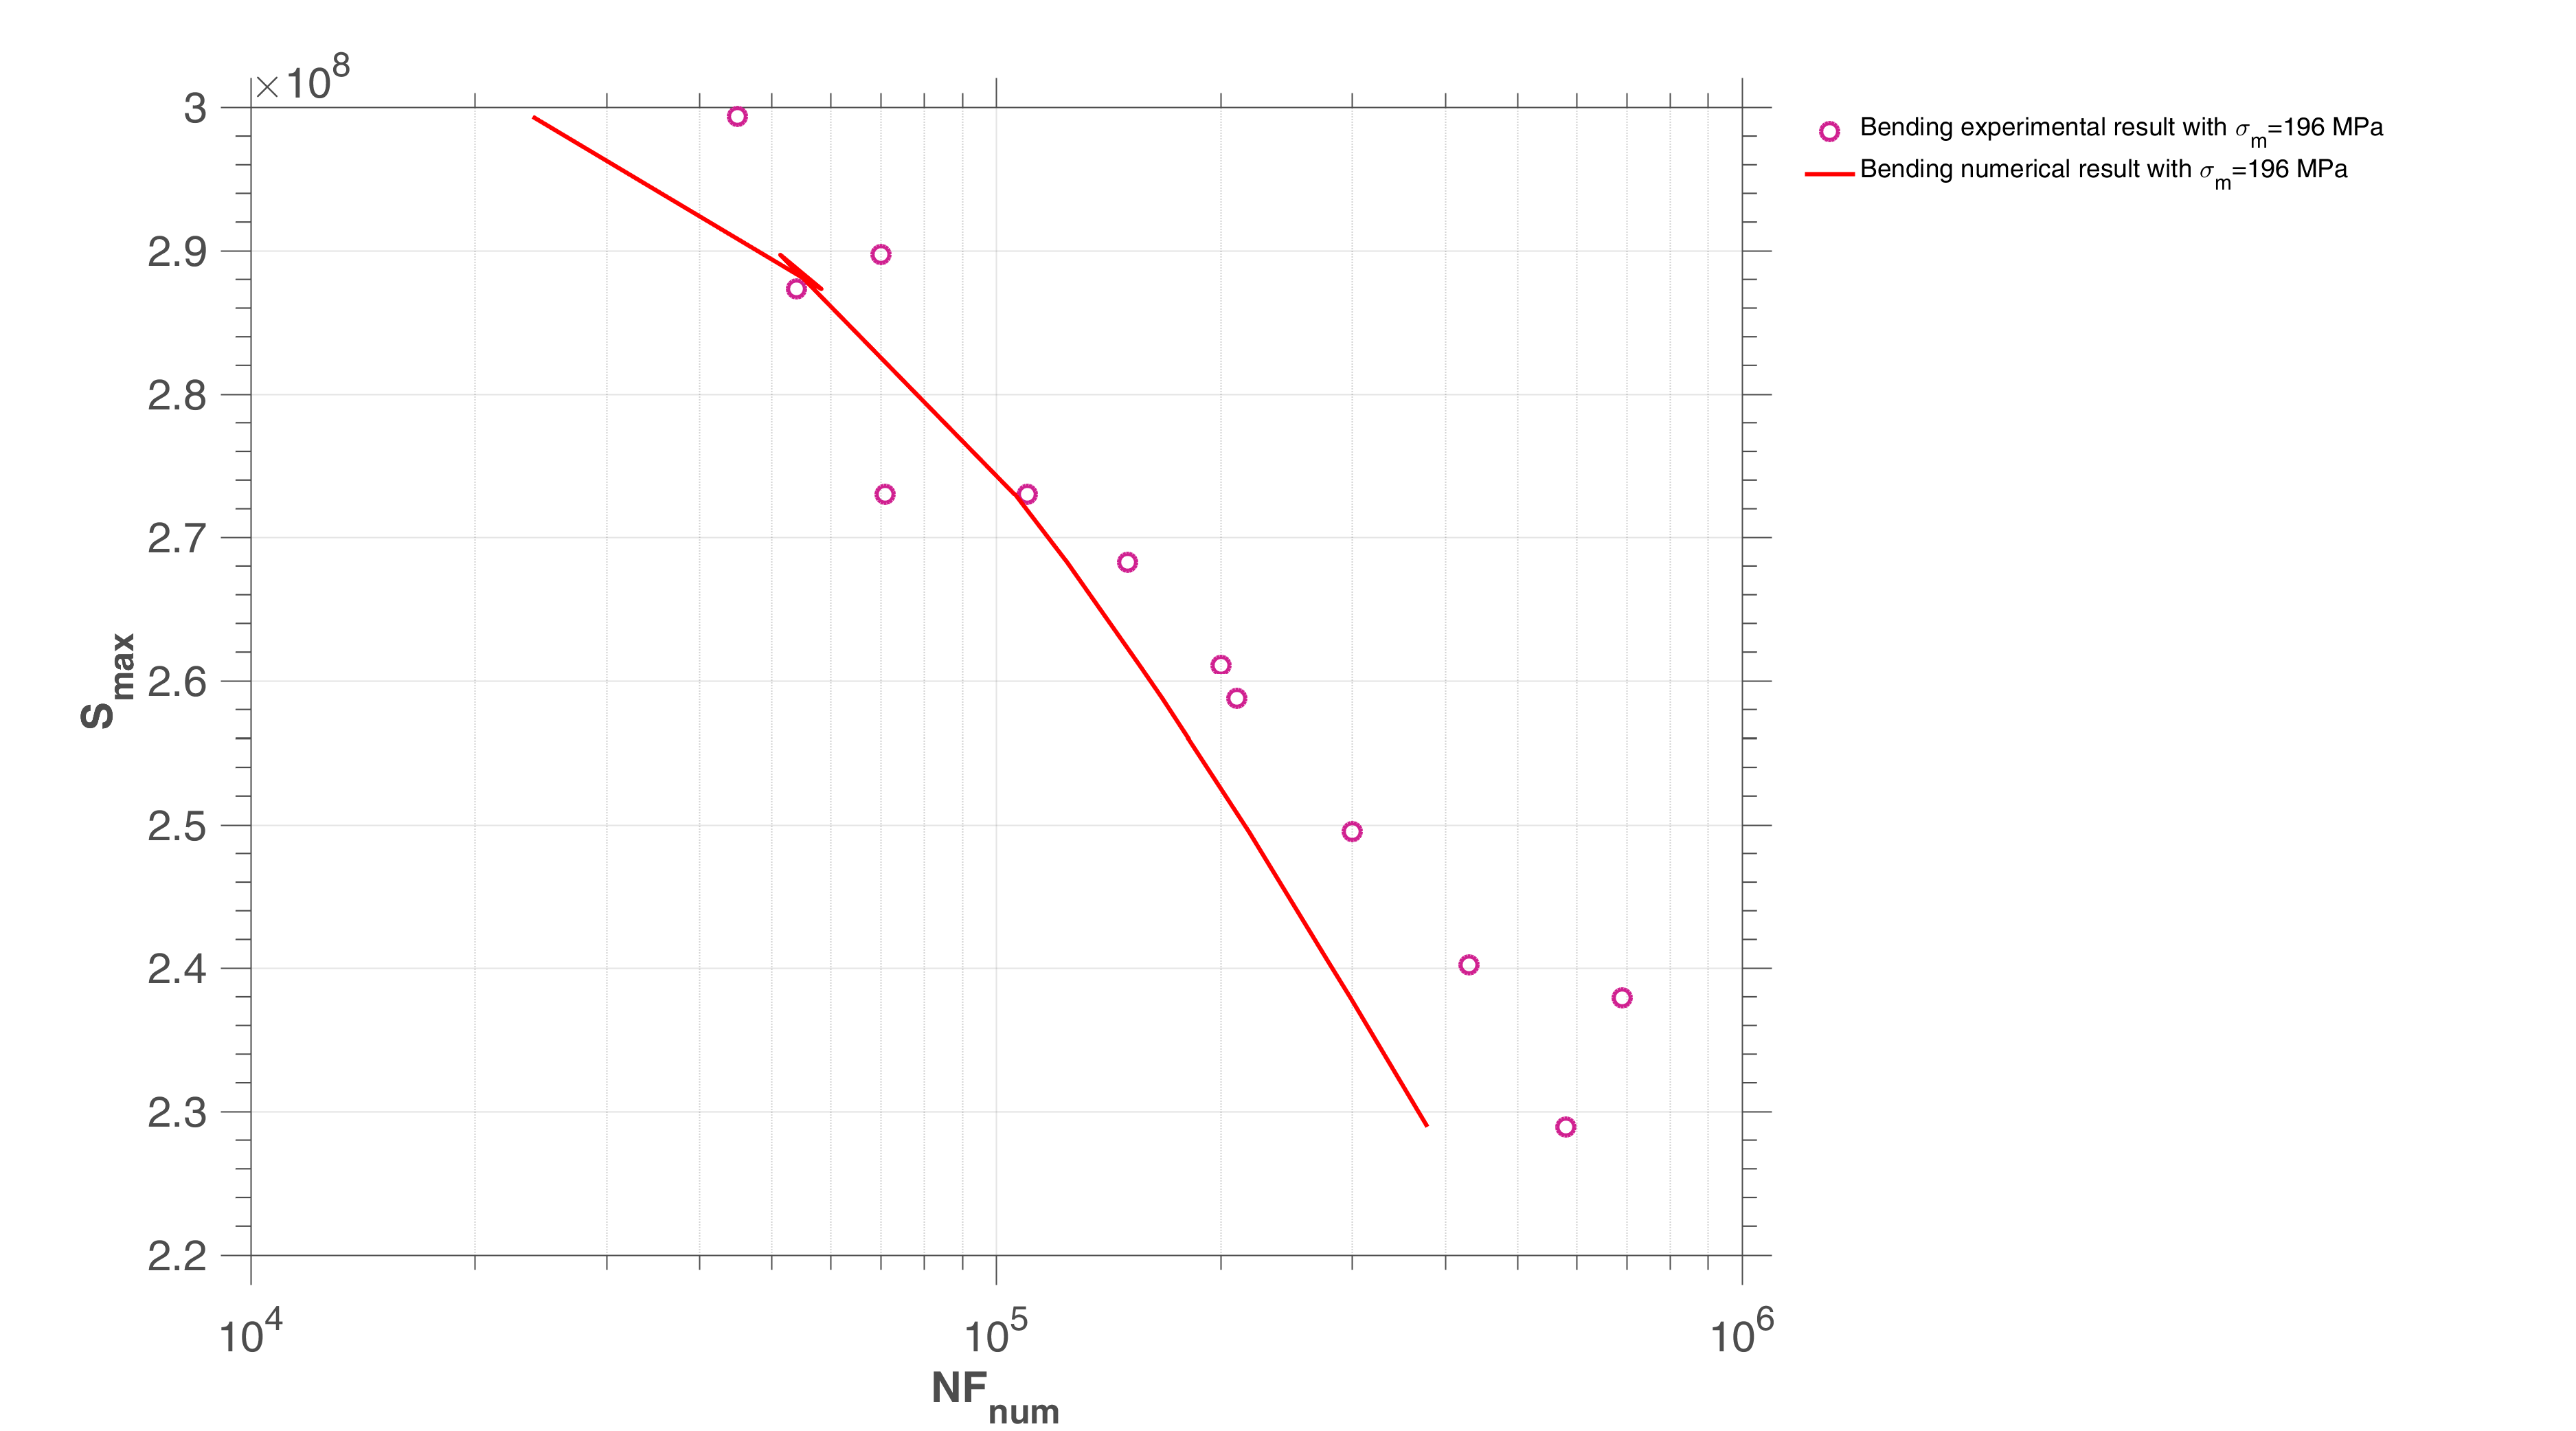
\includegraphics[width=\textwidth]{figures//b1D_m_SM45C_sn.png} 
	\caption{Bending test with mean stress on SM45C steel(R=-1,$\sigma_m=196 MPa$)}
	\label{fig.b1DmSM45Csn}
\end{figure}
\begin{figure}[!h]
	\centering
	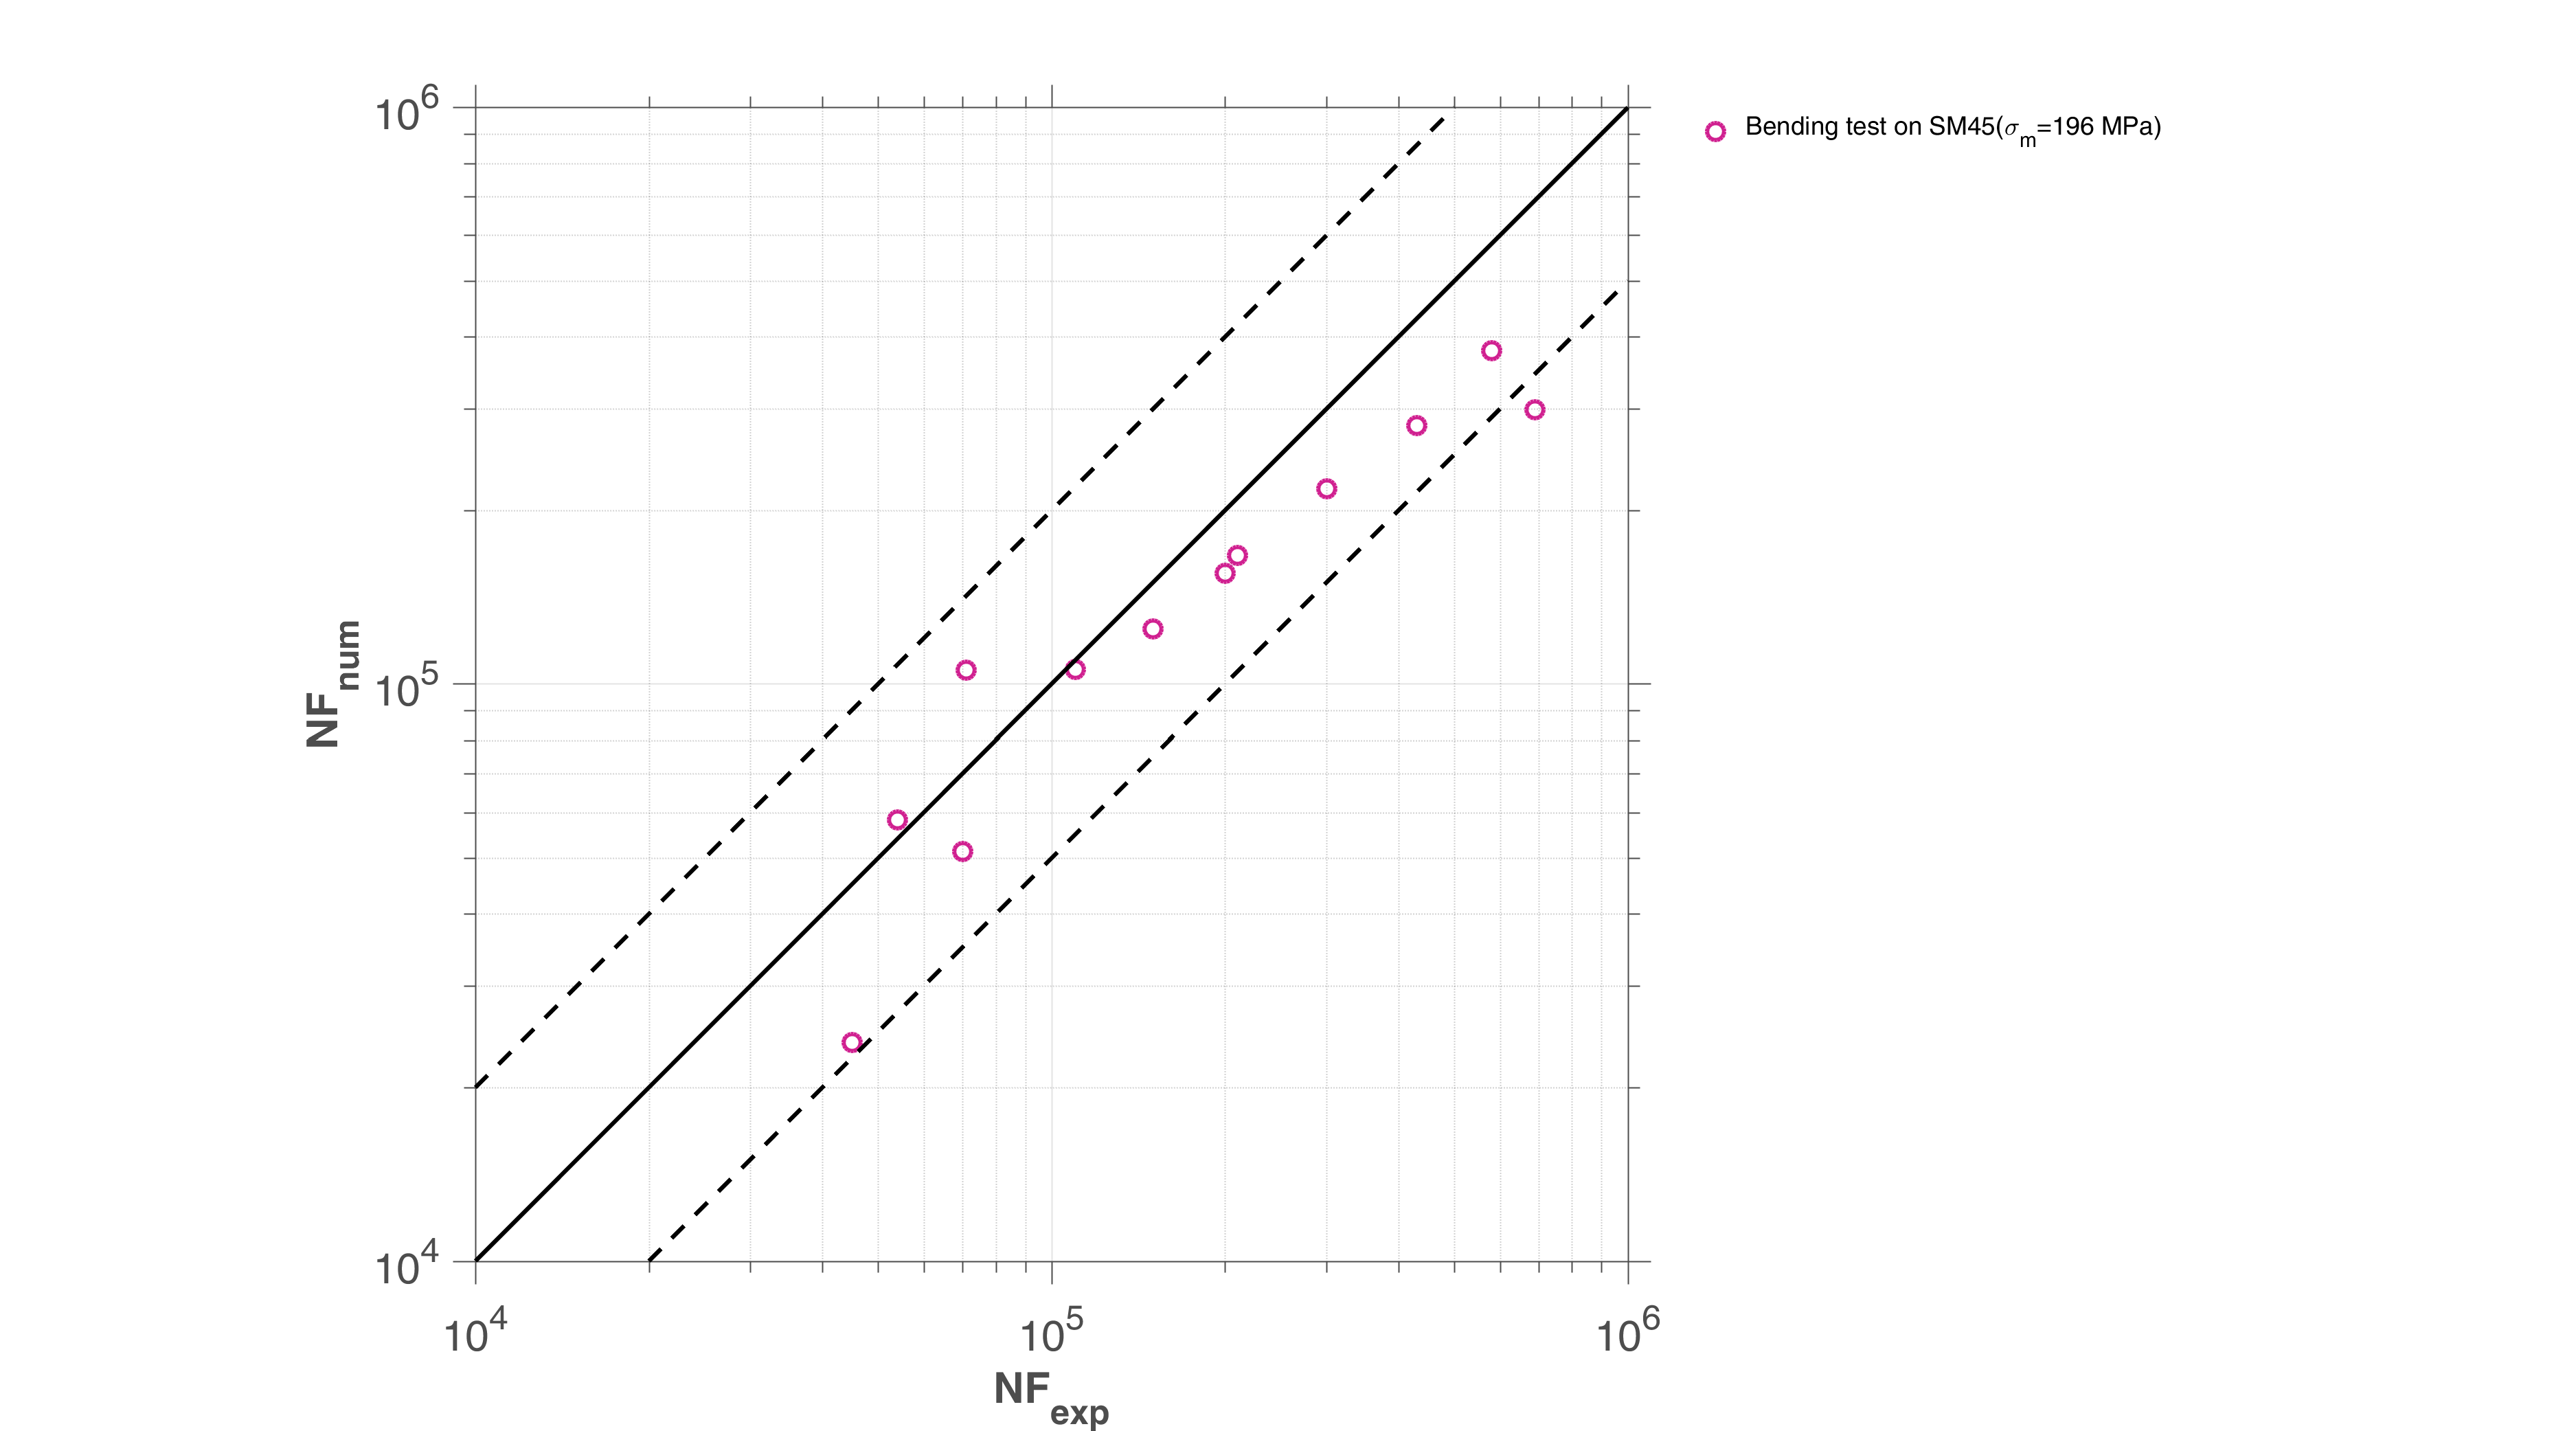
\includegraphics[width=\textwidth]{figures//b1D_m_SM45C_err1.png} 
	\caption{Bending test with mean stress on SM45C steel(R=-1,$\sigma_m=196 MPa$)}
	\label{fig.b1DmSM45Cerr1}
\end{figure}

\begin{figure}[!h]
	\centering
	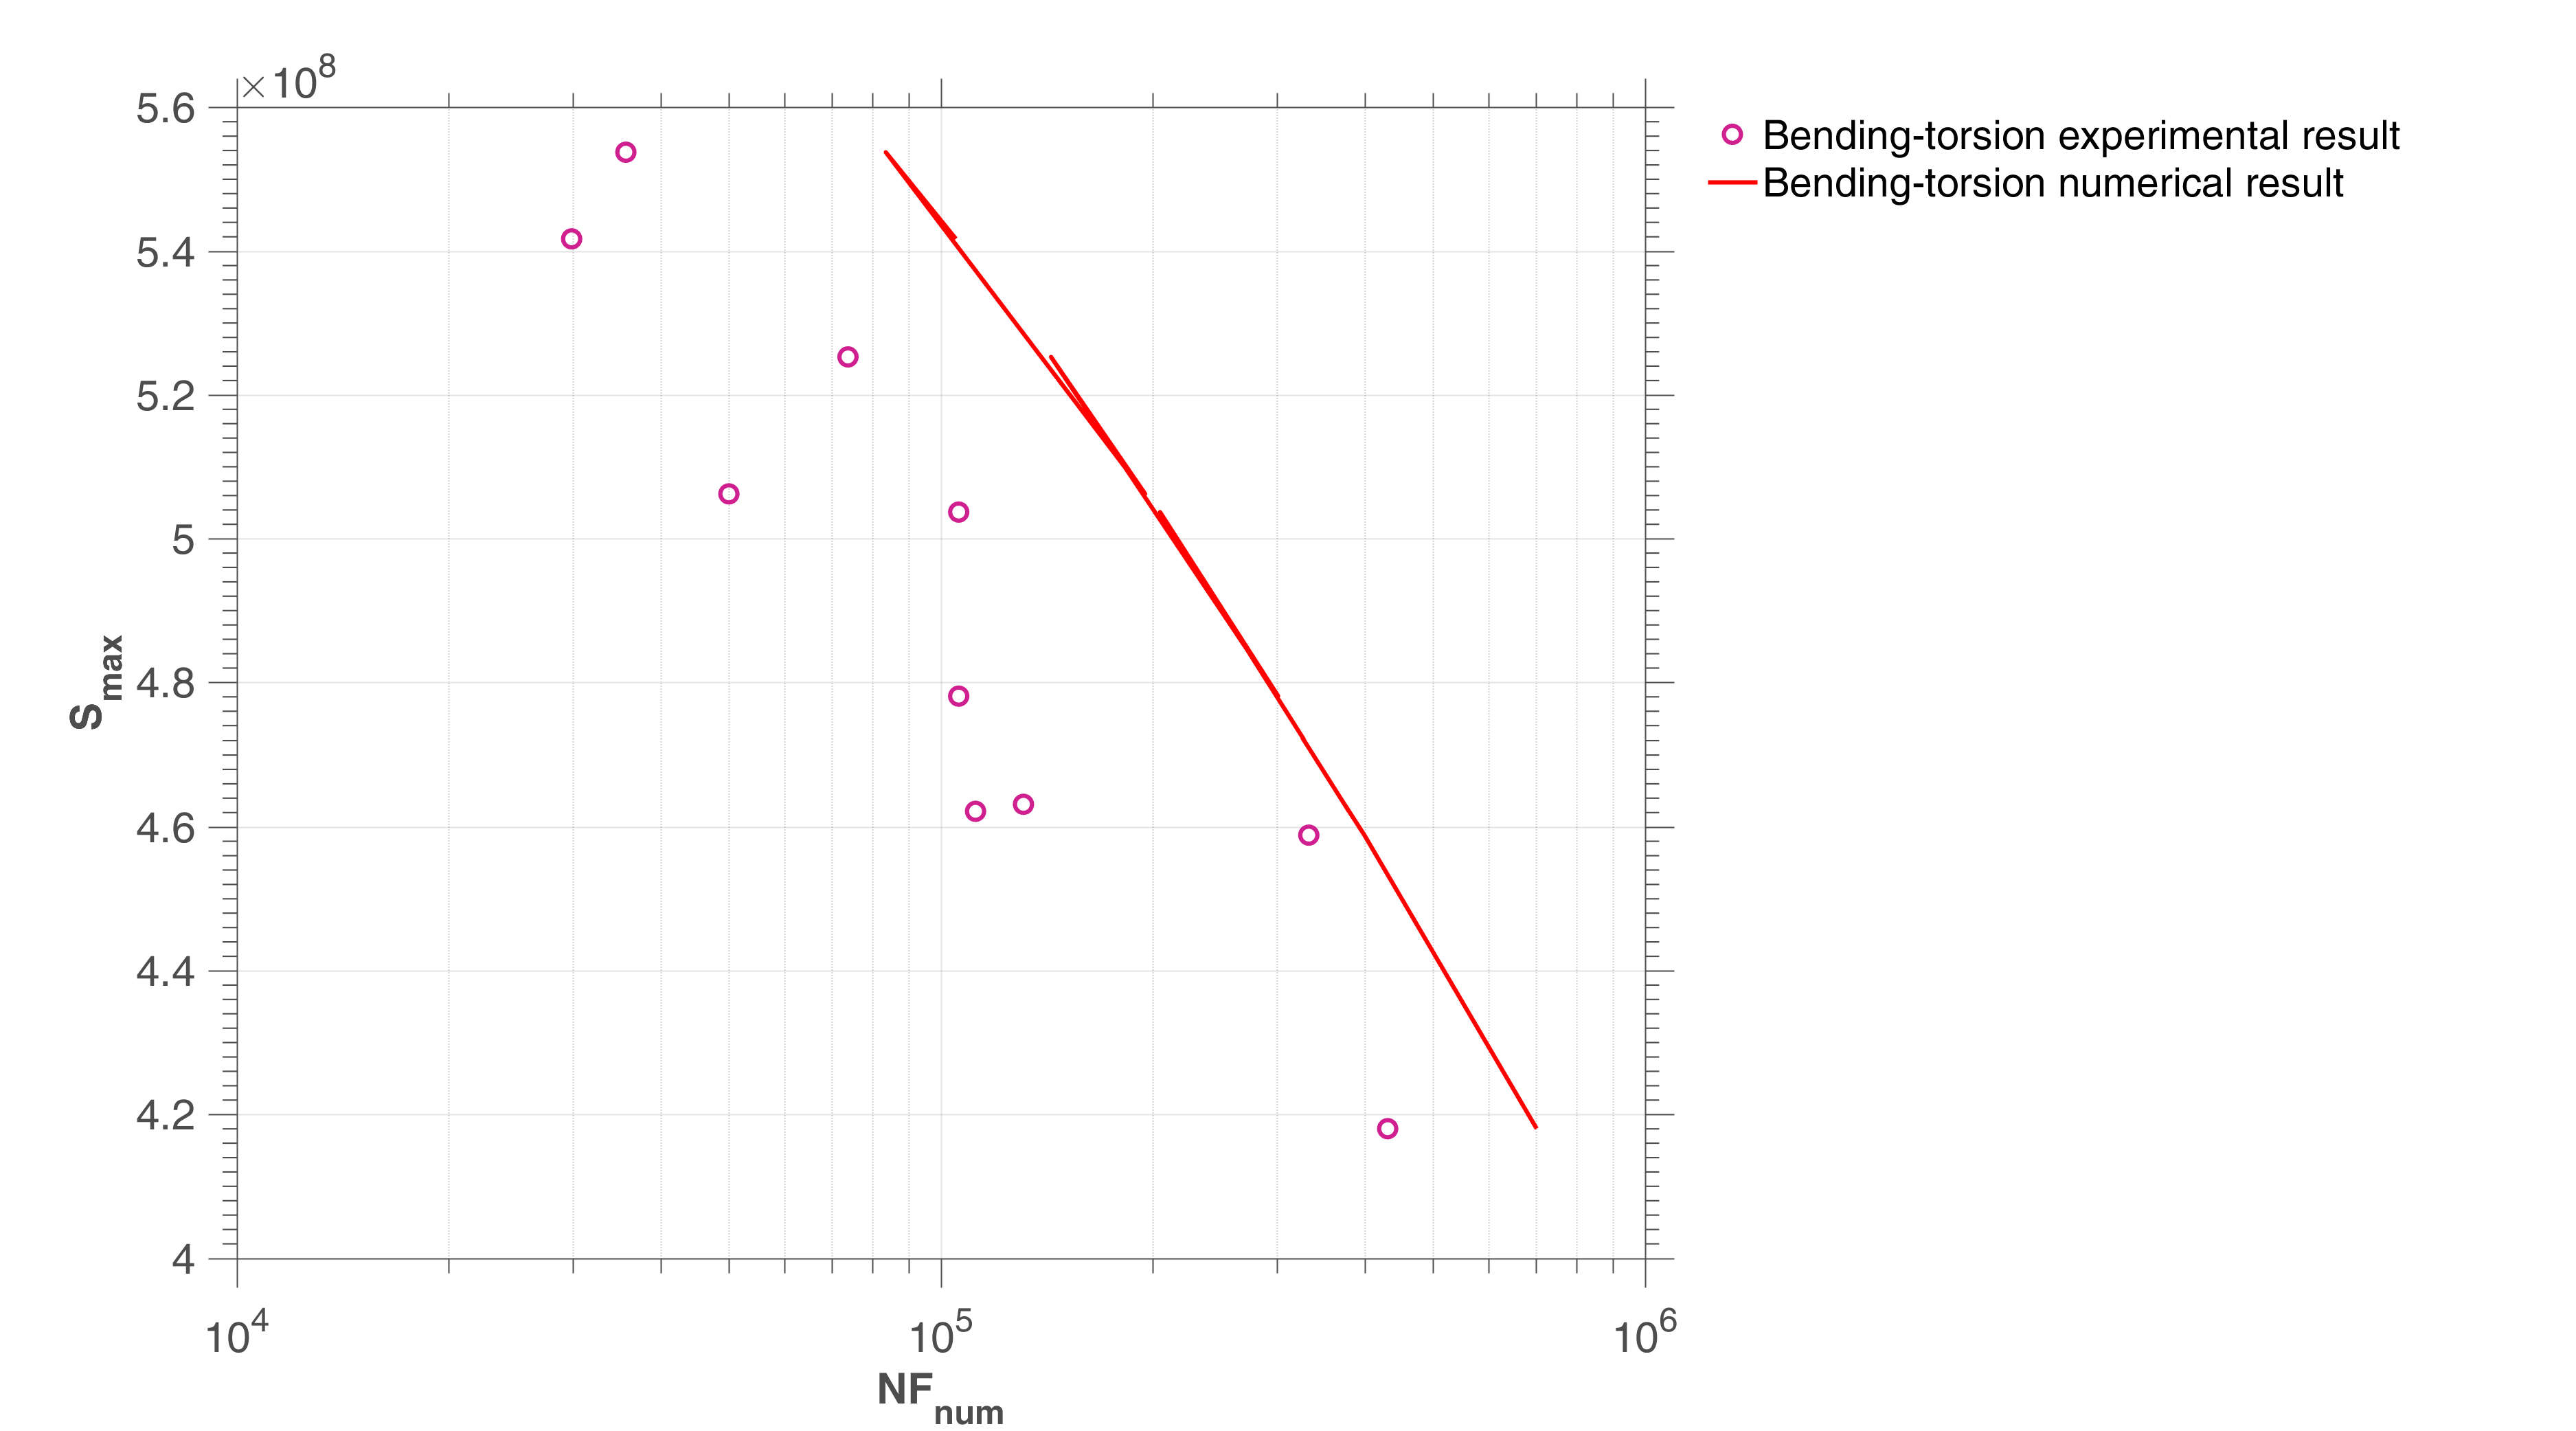
\includegraphics[width=\textwidth]{figures//bt2D_SM45C_sn.png} 
	\caption{Calibrated S-N curve of SM45C steel under fully reversed bending-torsion tests}
	\label{fig.bt2DSM45Csn}
\end{figure}
\begin{figure}[!h]
	\centering
	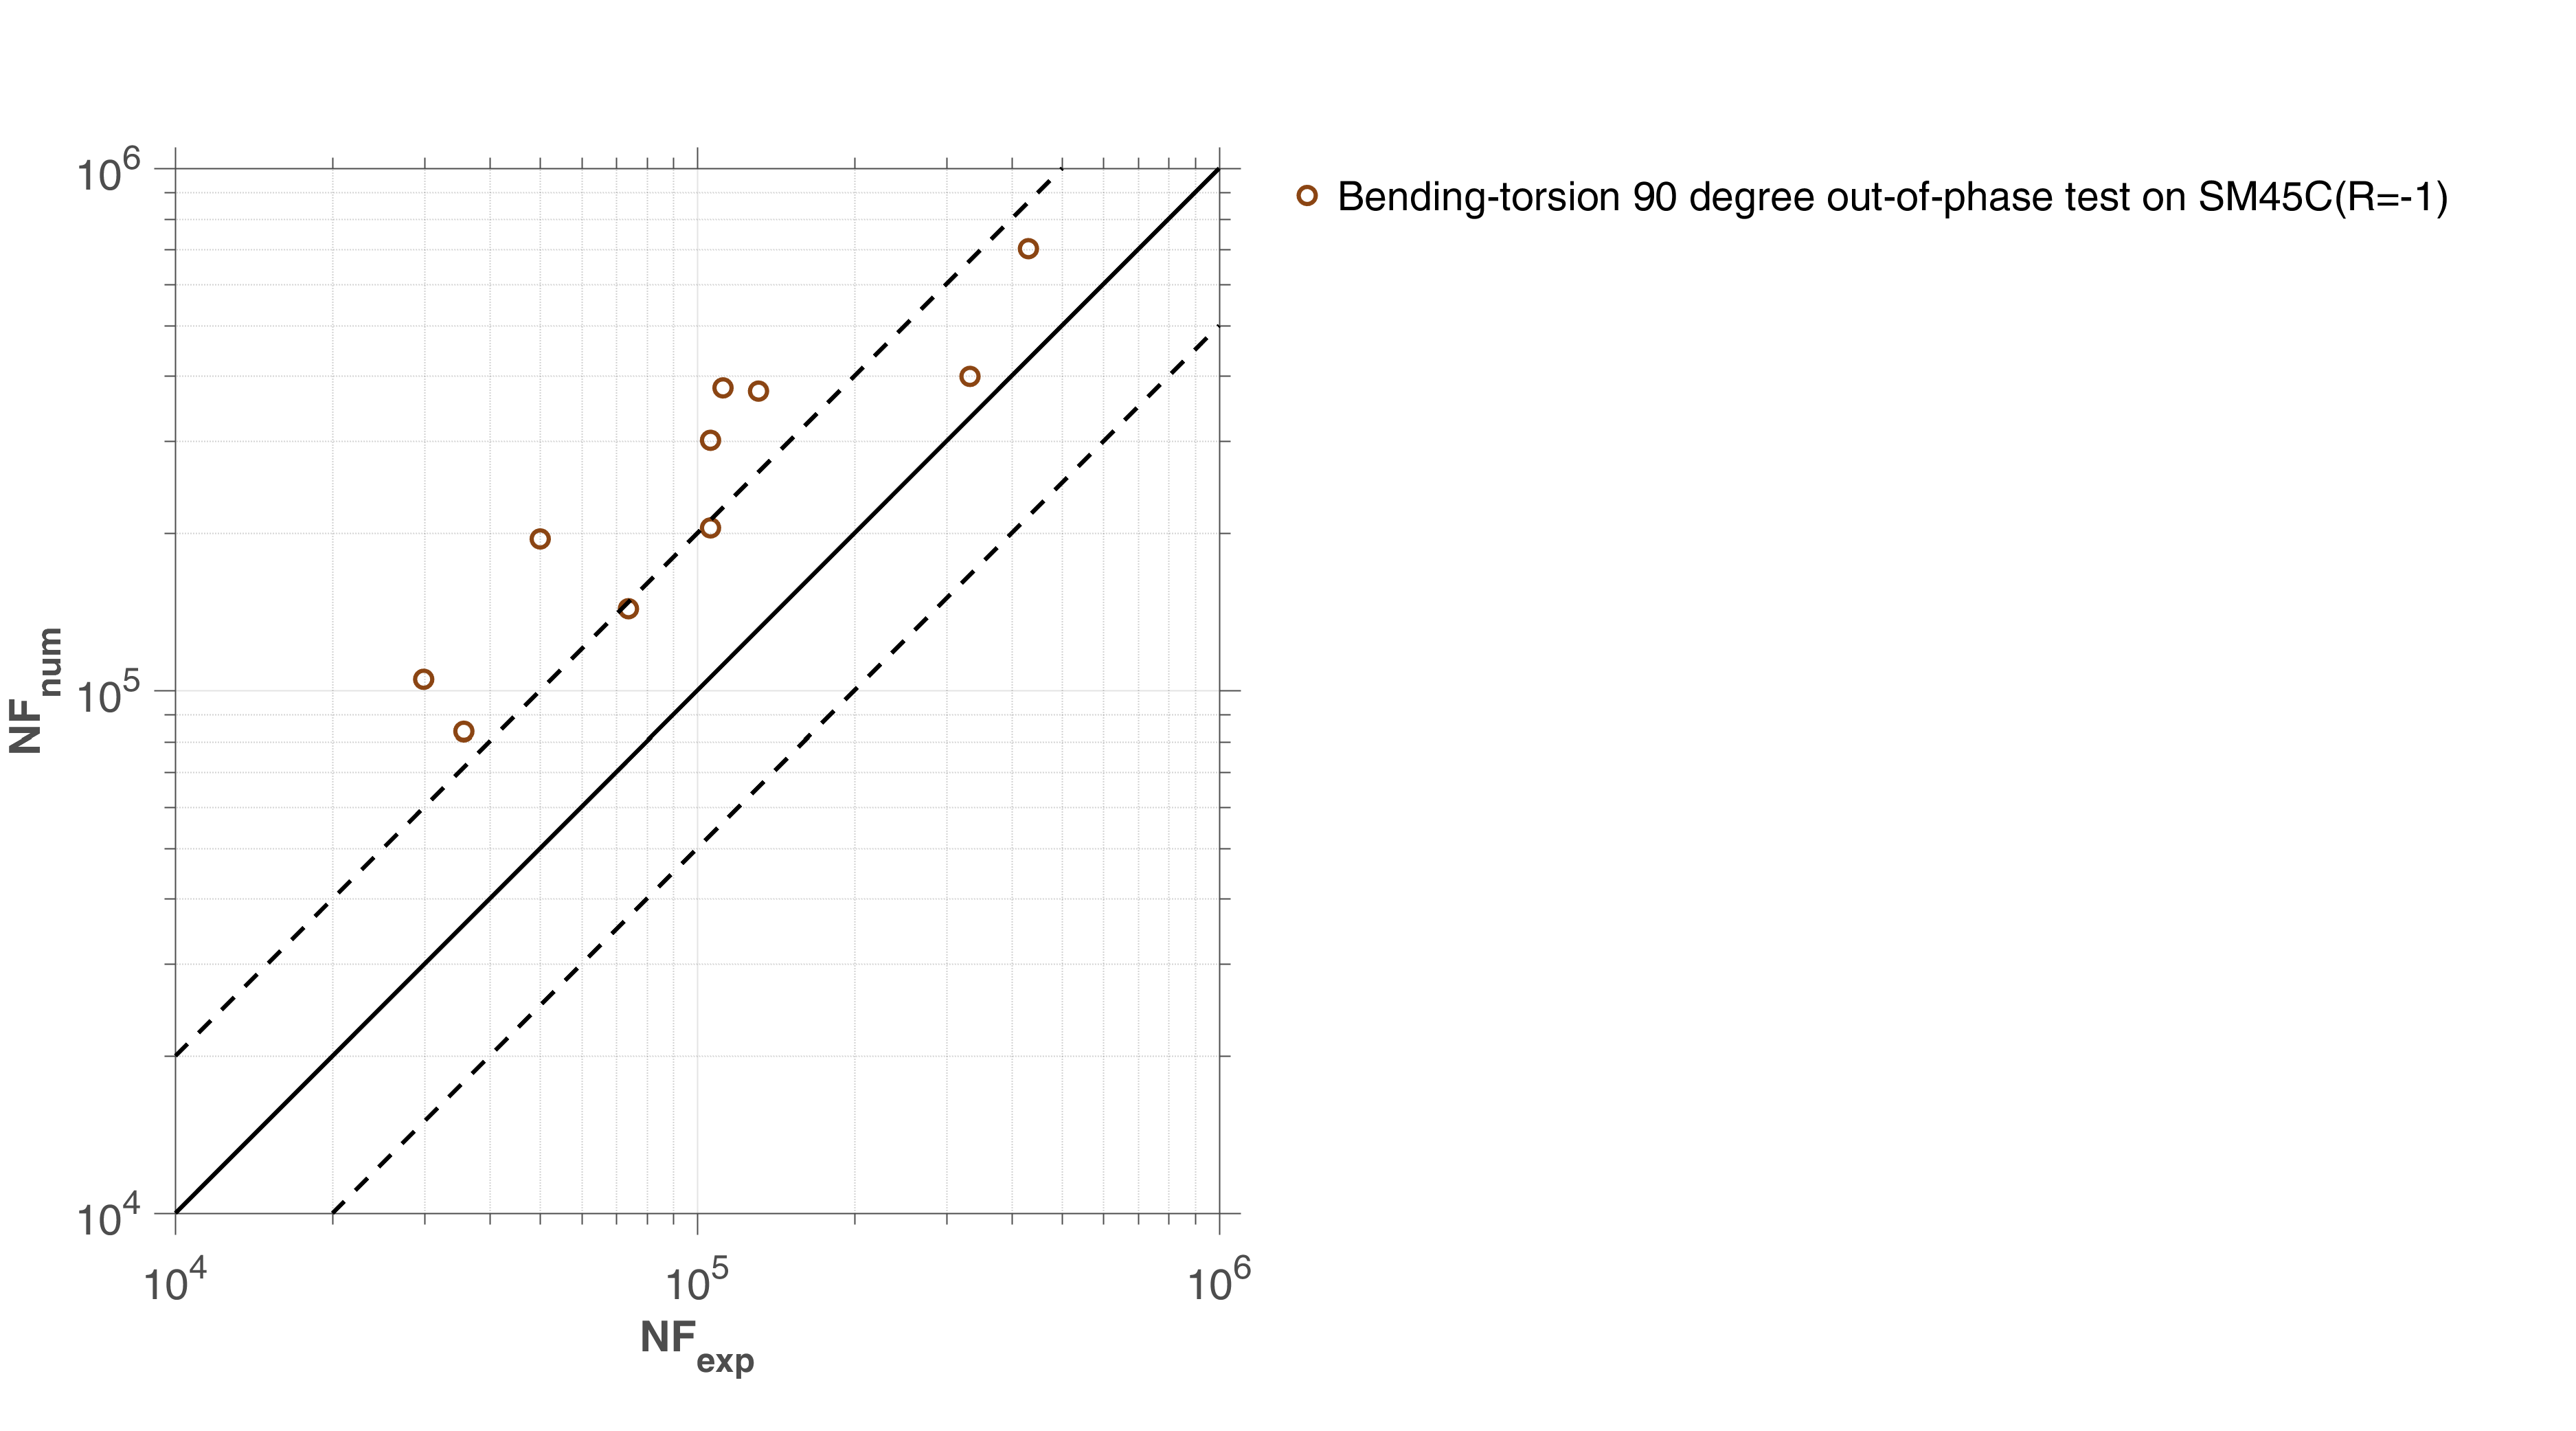
\includegraphics[width=\textwidth]{figures//bt2D_SM45C_err1.png} 
	\caption{Calibrated S-N curve of SM45C steel under fully reversed bending-torsion tests}
	\label{fig.bt2DSM45Cerr1}
\end{figure}
\begin{figure}[!h]
	\centering
	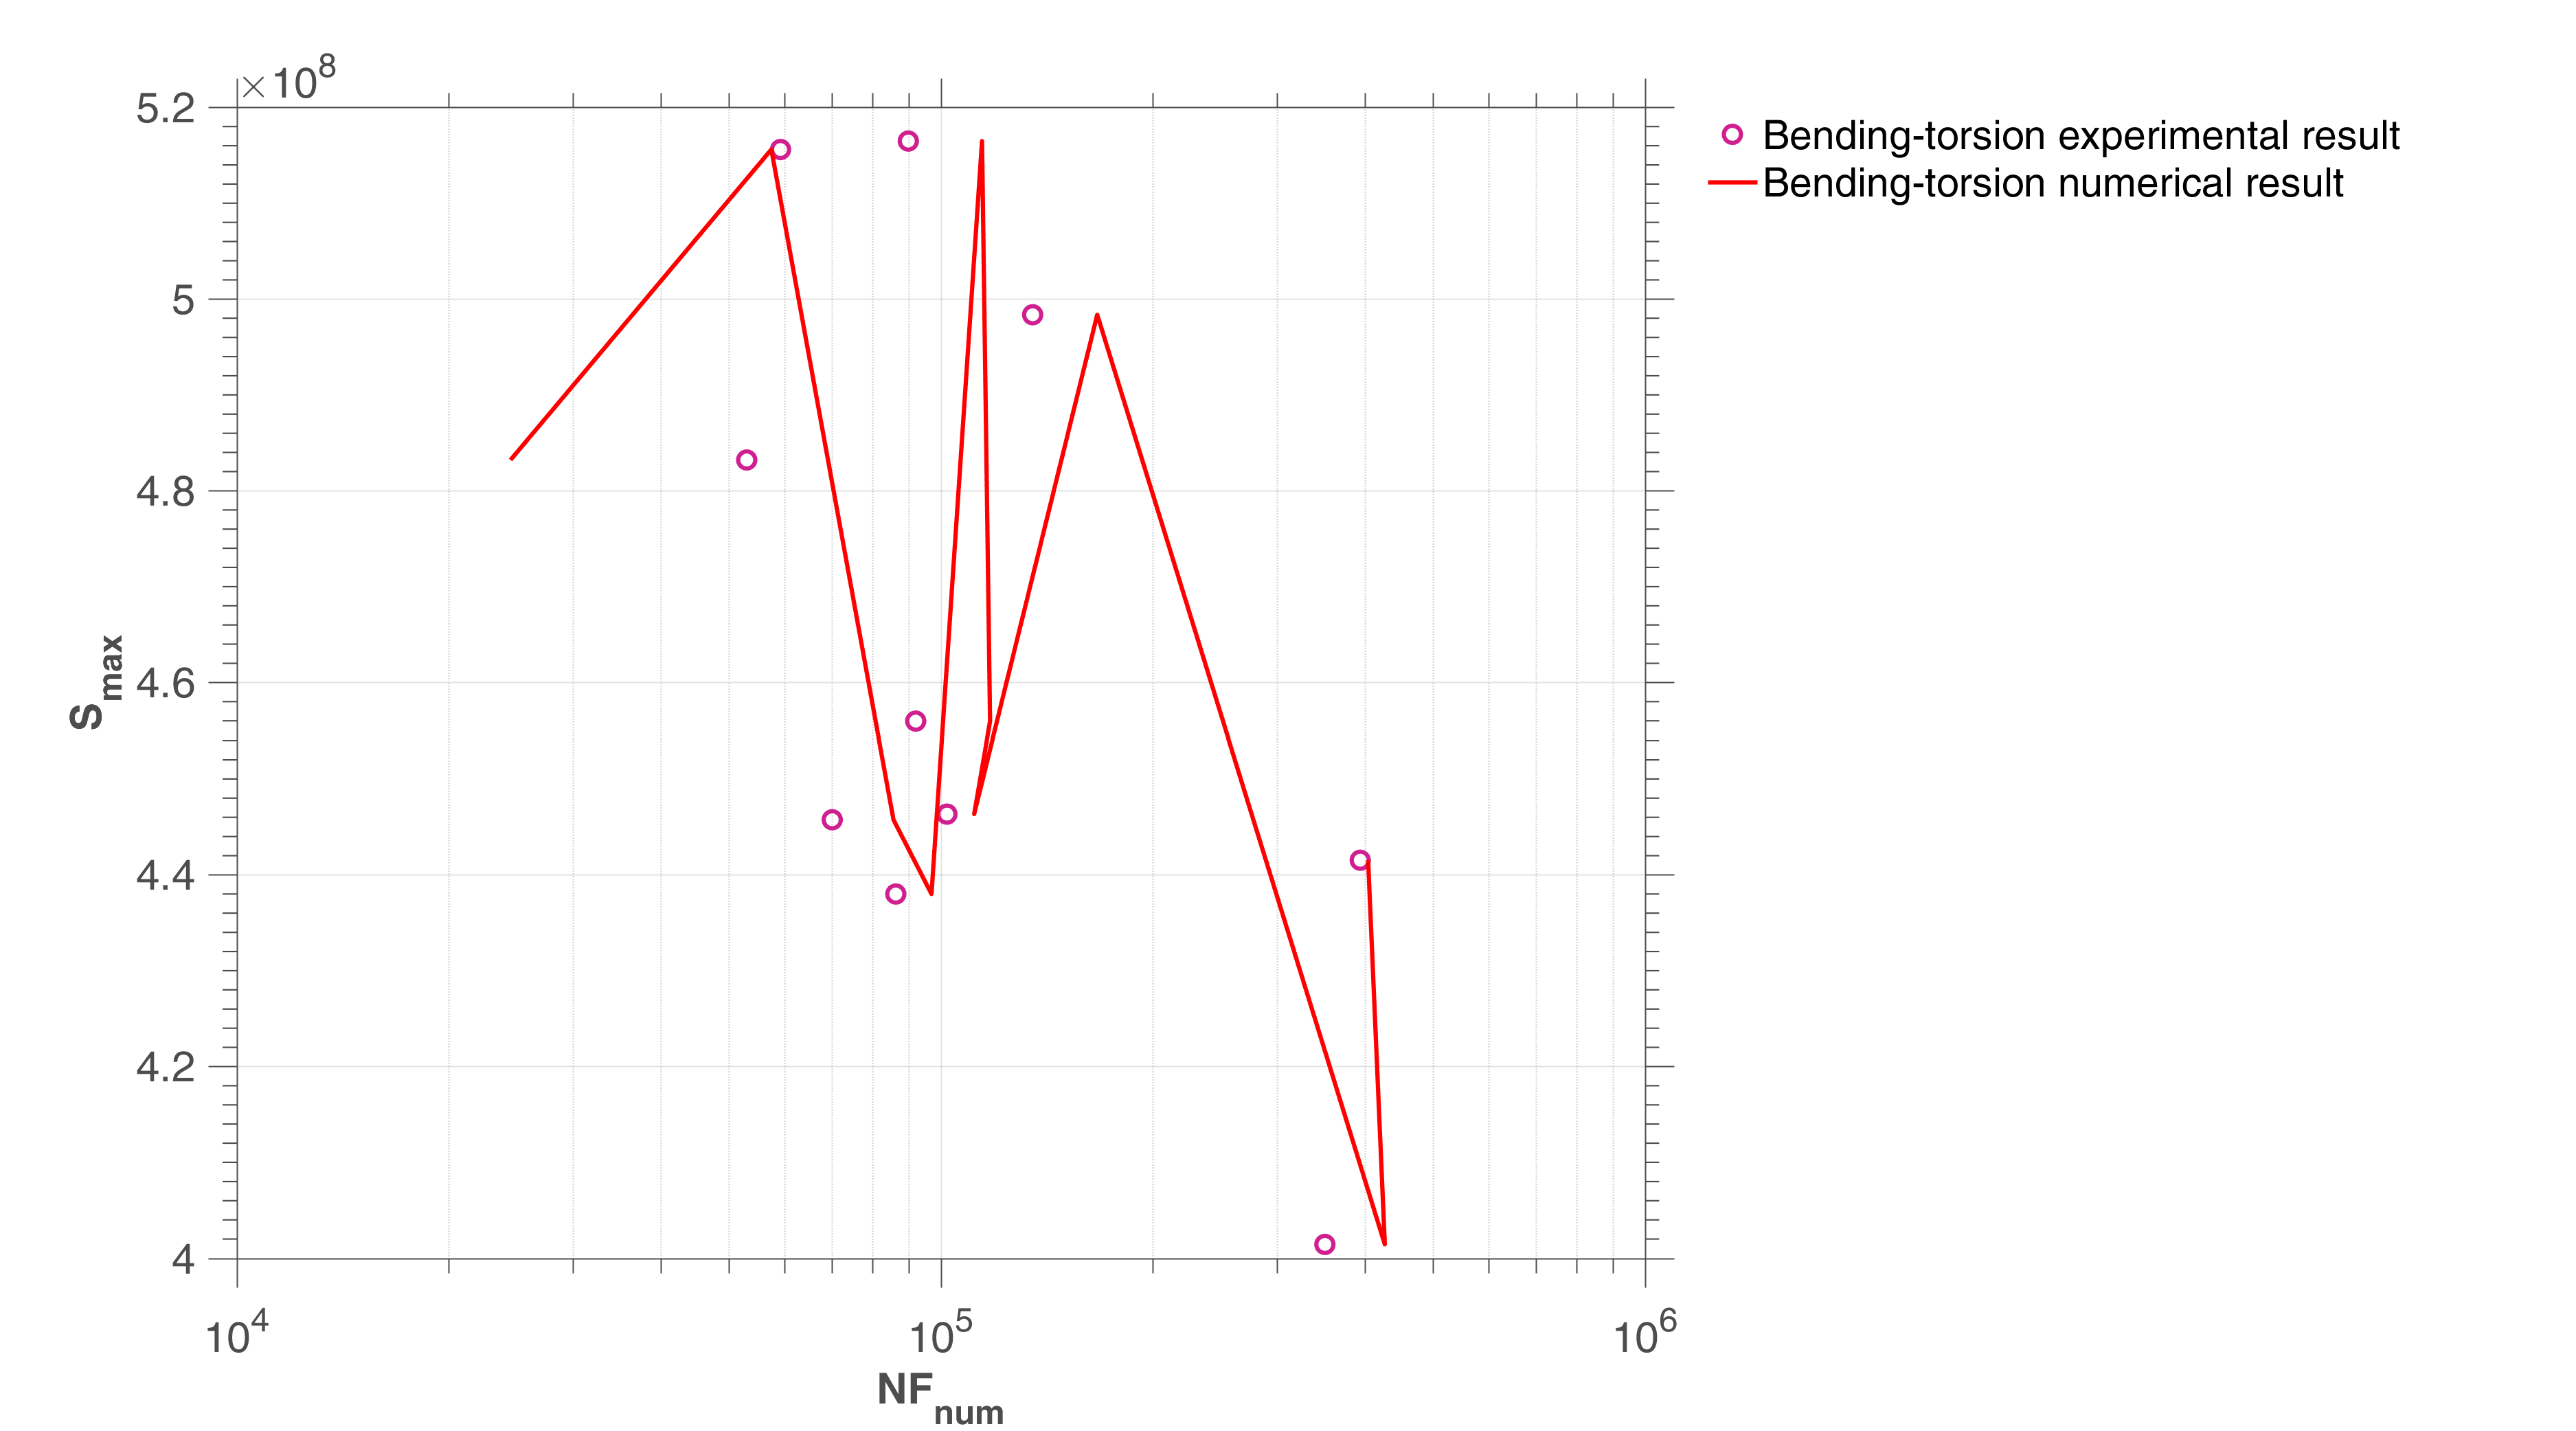
\includegraphics[width=\textwidth]{figures//bt2D_m_SM45C_sn.png} 
	\caption{Calibrated S-N curve of SM45C steel under fully reversed bending-torsion tests with mean stress}
	\label{fig.bt2DmSM45Csn}
\end{figure}
\begin{figure}[!h]
	\centering
	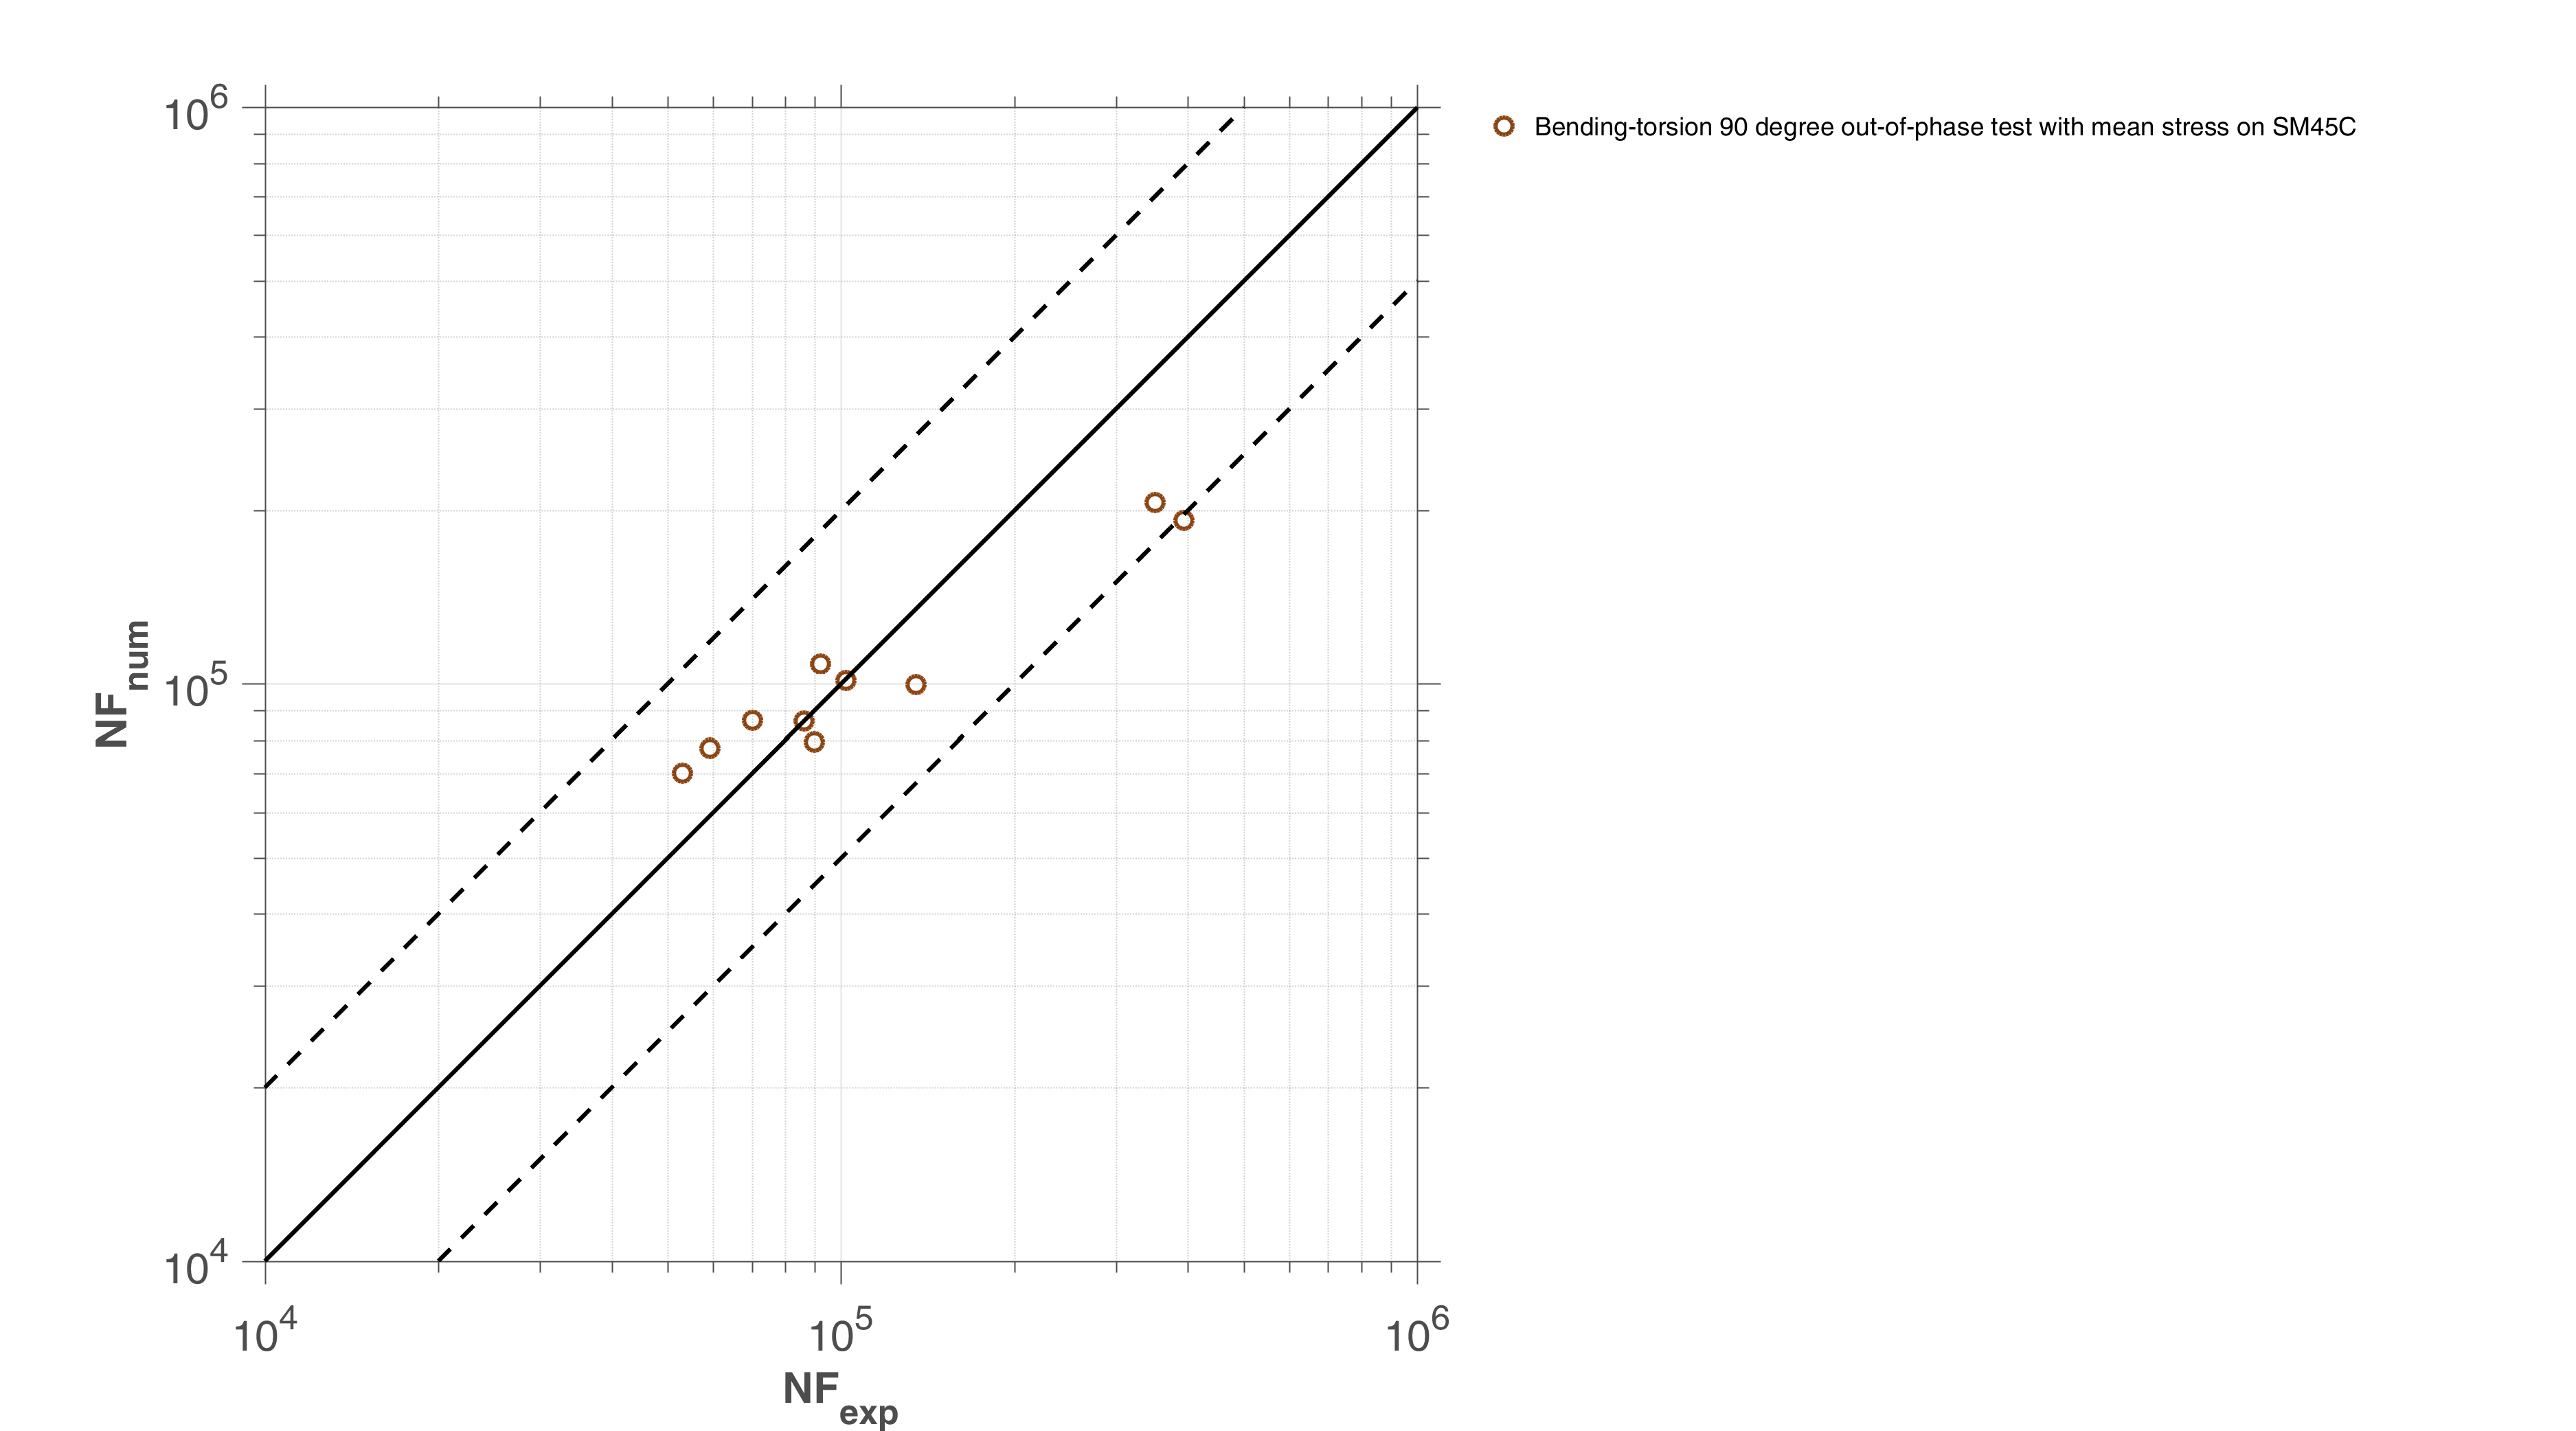
\includegraphics[width=\textwidth]{figures//bt2D_m_SM45C_err1.png} 
	\caption{Calibrated S-N curve of SM45C steel under fully reversed bending-torsion tests with mean stress}
	\label{fig.bt2DmSM45Cerr1}
\end{figure}

\begin{comment}
\subsection{Experimental validation of the model on ER7(clement roux thesis without $\sigma_{-1}$)}
This part is for the goal of complete the fatigue data in order to choose a method to calculate the fatigue life adapted to our situation(multiaxial stress trajectory with out of phase load). The material constants are shown in Table.\ref{tab:ER7}.
\begin{table}[!h]
	\centering
	\begin{tabular}{ll}
		\hline
		\textbf{Parameters}                                       & \textbf{Value}                    \\ \hline
		Young's modulus                                          & $E=214$ GPa                       \\
		Macroscopic yield stress                              & $\sigma_y=405$ MPa              \\
		Ultimate stress                  & $\sigma_u=720$ MPa                        \\ \hline
	\end{tabular}
	\caption{Material parameters}
	\label{tab:ER7}
\end{table}
\end{comment}

\clearpage
\subsection{Experimental validation of the model on 10 HNAP steel}
\subsubsection{Presentation of the material}
Fatigue tests were performed on the HNAP steel. It is a very low carbon steel
which resembles the 10 CN 6. In Table.\ref{tab.10HNAPchem}, its chemical composition is given:	
	\begin{table}[!h]
		\centering
		\begin{tabular}{rrrrrrrrr}
			\hline
			C      & Mn     & Si     & P      & S      & Cr     & Cu     & Ni     & Fe       \\
			0.12\% & 0.71\% & 0.41\% & 0.08\% & 0.03\% & 0.81\% & 0.30\% & 0.50\% & the rest \\ \hline
		\end{tabular}
		\caption{Chemical composition of 10 HNAP steel\cite{Bedkowski1994}}
		\label{tab.10HNAPchem}
	\end{table}
The mechanical properties of this steel are given in Table.\ref{tab.10HNAPmec}:
\begin{table}[!h]
	\centering
	\begin{tabular}{rrrrr}
		\hline
		$Re_{0.2\%}$ & $R_m$   & A    & $\nu$ & E          \\
			418 MPa     & 566 Mpa & 32\% & 0.29  & 215000 Mpa \\ \hline
			\end{tabular}
			\caption{Mechanical characteristics of steel 10 HNAP\cite{Bedkowski_1994}}
			\label{tab.10HNAPmec}
			\end{table}
		
where 
\begin{table}[!h]
	\centering
	\begin{tabular}{ll}
		$\Sigma_e$ & : elastic limit at 0.2\% of plastic deformation, \\
		$R_m$      & : maximum tensile strength,                                                                  \\
		A          & : elongation at break,                                                                       \\
		$\nu$      & : Poisson's coefficient,                                                                     \\
		E          & : Young's modulus.                                                                          
	\end{tabular}
\end{table}

\subsubsection{Description of fatigue tests on 10 HNAP steel}
The Macha team performed a large number of fatigue tests on the HNAP steel. Thus, it performed not only simple tensile compression and torsion tests (R = -1) in order to establish The corresponding Wöhler curves but also tests under variable loading on cylindrical specimens of the same material\cite{ACHTELIC1994}. VIDAL\cite{VIDAL1996} carried out tensile tests on this material for various mean stress values. It has established the Wöhler curve in repeated traction in order to validate on this steel the method of Robert whose use requires three Wöhler curves in symmetrical alternating traction, symmetrical alternating torsion and repetitive traction.

\vspace{6pt}
\noindent
\textbf{Wöhler curve in tension-compression}

The model chosen by Macha and recovered by Jabbado\cite{jabbado:pastel-00002116} for the tensile-compression Wöhler curve is that of Basquin:
\begin{equation}
lnN=68.361 − 9.82ln\left( \sigma_{-1}\right) 
\end{equation}

\noindent
\textbf{Wöhler curve in symmetrical alternating torsion}

The symmetric alternating torsion Wöhler curve was recovered by Jabbado\cite{jabbado:pastel-00002116} using following equation:
\begin{equation}
lnN=21.55 − 0.0385\tau_{-1}
\end{equation}

\noindent
\textbf{Tensile fatigue tests for various mean stress values}

VIDAL\cite{VIDAL1996} carried out tensile tests on HNAP steel for various values of mean stress. The results are summarized in Table.\ref{tab.10HNAPmean}. They allowed us to plot the Wöhler curves for different values of the mean stress $\sigma_m$. These curves are modeled by the Wöhler equation:
\begin{equation}
lnN=A − B\sigma_{max}
\label{eq.10HNAPmean}
\end{equation}
In the Table.\ref{tab.10HNAPAB}, the values of the constants A and B of Eq.\eqref{eq.10HNAPmean}.
\begin{table}[!h]
	\centering
	\begin{tabular}{ccl}
		\hline
		\multicolumn{1}{l}{$\sigma_a$(MPa)} & \multicolumn{1}{l}{$\sigma_m$(MPa)} & $N_{exp}$(cycles)    \\ \hline
		250                                 & 75                                  & 439300;402500        \\
		270                                 & 75                                  & 358200;854700;318700 \\
		290                                 & 75                                  & 252300;376300;379700 \\
		310                                 & 75                                  & 54800;123400;45000   \\ \hline
		250                                 & 150                                 & 157400;1333000       \\
		270                                 & 150                                 & 172100;121500;233100 \\
		290                                 & 150                                 & 124300;41900;60500   \\ \hline
		230                                 & 225                                 & 413900;204500;545200 \\
		250                                 & 225                                 & 122400;229600;104000 \\
		270                                 & 225                                 & 110000;29900;66000   \\ \hline
		190                                 & 300                                 & 497100;234300;524800 \\
		210                                 & 300                                 & 463500;367300;259500 \\
		230                                 & 300                                 & 219000;179400;222400 \\
		250                                 & 300                                 & 95300;118200;59100   \\ \hline
	\end{tabular}
	\caption{Experimental results of tensile tests for various values of $\sigma_m$}
	\label{tab.10HNAPmean}
\end{table}




\noindent
\textbf{Fatigue testing under variable loading}

Random multiaxial loading fatigue tests were performed on cylindrical HNAP steel specimens\cite{ACHTELIC1994}. The load considered is proportional and results from a combination of bending and torsion. The random signal is stationary and has a normal distribution as a probability distribution. Tests of this type have been analyzed and simulated by Carpinteri et al.\cite{carpinteri2003multiaxial}. They were provided to us in the form of tests carried out on the HNAP steel for two values of the angle $\alpha'$: $\alpha' = \pi / 8$ and $\alpha' = \pi / 4$ . $\alpha' $ is the angle made by the resultant moment $M$ with the bending moment $M_B$ (see \figref{fig.10HNAPsample}).

\begin{figure}[!h]
	\centering
	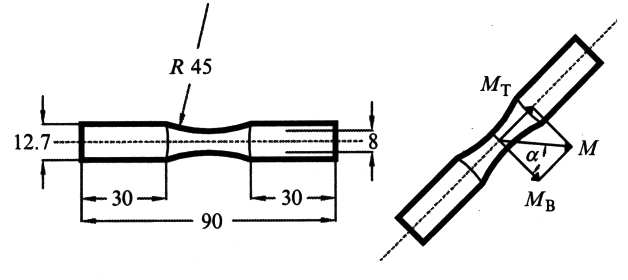
\includegraphics[width=0.7\textwidth]{figures//10HNAPsample.png} 
	\caption{Bending-torsion fatigue tests on cylindrical specimens\cite{carpinteri2003multiaxial}}
	\label{fig.10HNAPsample}
\end{figure}

The stationary random loading sequence contains 49152 values recorded by a time interval of 0.00375 seconds (frequency = 266.67 Hz). It is shown in \figref{fig.10HNAPrandom}. Its total duration is 184.32 seconds. This sequence is multiplied by load coefficients corresponding to bending $f (\sigma_{xx})$ and torsion $f (\tau_{xy})$ in order to obtain random multiaxial loading sequences. As the signal is stationary, the breaking life is determined in terms of number of sequences with break $N_{Sq}$. Knowing $N_{Sq}$ and the total time in seconds of the sequence studied, it is easy to express the lifetime of the piece in seconds. The results of fatigue tests under variable loads are summarized in Table.\ref{tab.10HNAPrand1} and Table.\ref{tab.10HNAPrand2} as a function of angle $\alpha'$ and ratio r; $r =f(\tau_{xy})/f(\sigma_{xx})$.
\begin{figure}[!h]
	\centering
	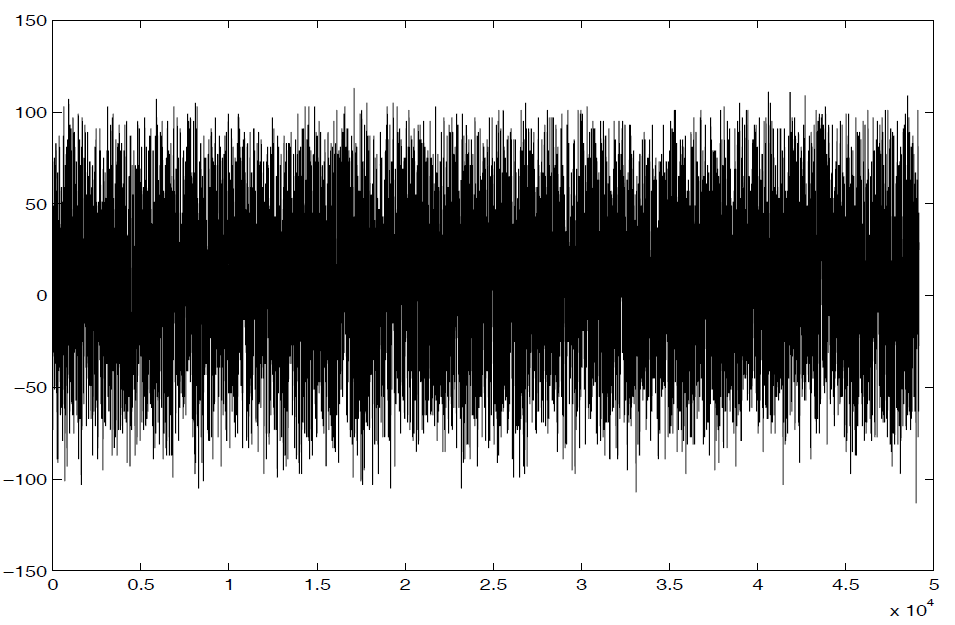
\includegraphics[width=0.8\textwidth]{figures//10HNAPrandom.png} 
	\caption{Bending-torsion fatigue tests on cylindrical specimens\cite{carpinteri2003multiaxial}}
	\label{fig.10HNAPrandom}
\end{figure}

\textbf{1st type of tests:} $\alpha' = \pi / 8$ and $r =f(\tau_{xy})/f(\sigma_{xx})=0.2$.

\begin{table}[!h]
	\centering
	\begin{tabular}{lrrrr}
		\hline
		$N^o$ & $f(\sigma_{xx})$ & $f(\tau_{xy})$ & $r$   & $T_{exp}(s)$ \\ \hline
		1     & 5.7084                  & 1.1822  & 0.2 & 16843.2    \\
		2     & 5.2917                  & 1.0959  & 0.2 & 17780.1    \\
		3     & 4.8337                  & 1.0010  & 0.2 & 24416.5    \\
		4     & 5.2674                  & 1.0909  & 0.2 & 24858.2    \\
		5     & 5.4534                  & 1.1294  & 0.2 & 26518.3    \\
		6     & 5.2002                  & 1.0769  & 0.2 & 36162.3    \\
		7     & 4.7944                  & 0.9929  & 0.2 & 47600.4    \\
		8     & 4.3862                  & 0.9084  & 0.2 & 57993.9    \\
		9     & 4.6241                  & 0.9576  & 0.2 & 60428      \\
		10    & 4.0194                  & 0.8324  & 0.2 & 73373.3    \\
		11    & 4.0127                  & 0.8310  & 0.2 & 87609.1    \\
		12    & 4.2292                  & 0.8758  & 0.2 & 89185.2    \\
		13    & 3.9213                  & 0.8121  & 0.2 & 106900     \\
		14    & 3.7731                  & 0.7814  & 0.2 & 117358     \\
		15    & 4.1148                  & 0.8521  & 0.2 & 118902     \\
		16    & 3.6150                  & 0.7486  & 0.2 & 132448     \\
		17    & 3.3135                  & 0.6862  & 0.2 & 170571     \\
		18    & 4.1298                  & 0.8553  & 0.2 & 178215     \\
		19    & 3.4761                  & 0.7199  & 0.2 & 225288     \\
		20    & 3.3430                  & 0.6923  & 0.2 & 352635     \\
		21    & 3.0135                  & 0.6241  & 0.2 & 355720     \\ \hline
	\end{tabular}
	\caption{Fatigue results under variable loads for $\alpha' = \pi / 8$ and $r =f(\tau_{xy})/f(\sigma_{xx})=0.2$}
	\label{tab.10HNAPrand1}
\end{table}

\textbf{2nd type of tests:} $\alpha' = \pi / 4$ and $r =f(\tau_{xy})/f(\sigma_{xx})=0.5$.

\begin{table}[]
	\centering
	\begin{tabular}{lrrrr}
		\hline
		$N^o$ & $f(\sigma_{xx})$ & $f(\tau_{xy})$ & $r$   & $T_{exp}(s)$ \\ \hline
		1   & 4.2519                  & 2.126   & 0.5 & 15379.4    \\
		2   & 4.0567                  & 2.0284  & 0.5 & 21465.7    \\
		3   & 3.8982                  & 1.9491  & 0.5 & 25350.4    \\
		4   & 3.7823                  & 1.8912  & 0.5 & 45949      \\
		5   & 3.5963                  & 1.7982  & 0.5 & 62434.8    \\
		6   & 3.4497                  & 1.7249  & 0.5 & 75225.7    \\
		7   & 2.9423                  & 1.4712  & 0.5 & 115009     \\
		8   & 2.8814                  & 1.4407  & 0.5 & 136794     \\
		9   & 2.3299                  & 1.165   & 0.5 & 203365     \\
		10  & 2.8399                  & 1.42    & 0.5 & 221370     \\
		11  & 2.8493                  & 1.4247  & 0.5 & 244757     \\
		12  & 2.2542                  & 1.1271  & 0.5 & 251723     \\
		13  & 2.3651                  & 1.1826  & 0.5 & 288080     \\
		14  & 2.4215                  & 1.2108  & 0.5 & 405444     \\ \hline
	\end{tabular}
	\caption{Fatigue results under variable loads for $\alpha' = \pi / 4$ and $r =f(\tau_{xy})/f(\sigma_{xx})=0.5$}
	\label{tab.10HNAPrand2}
\end{table}

In \figref{fig.10HNAP2Drandom}, an example of a random multiaxial loading sequence is given.
\begin{figure}[!h]
	\centering
	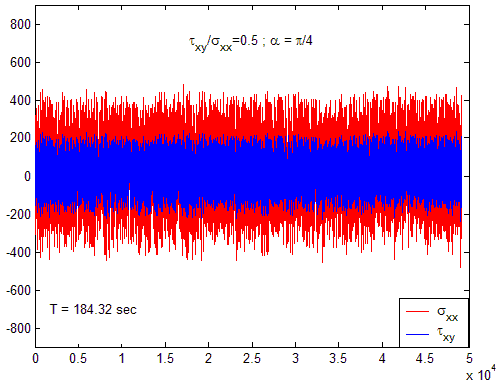
\includegraphics[width=0.8\textwidth]{figures//10HNAP2Drandom.png} 
	\caption{Multiaxial random loading sequence}
	\label{fig.10HNAP2Drandom}
\end{figure}

\subsubsection{Identification of model parameters of 10HNAP steel}
As mentioned earlier, the identification of the model parameters requires a Wöhler curve. This initiates the value of $\beta$, in the mean stress tests we have got the value of $\lambda$. And the value of $W_0$ and a comes from random loading. The parameters of the HNAP steel model can be identified by referring to Table.\ref{tab.10HNAP.para}. They are grouped in the following table:
\begin{table}[!h]
	\centering
	\begin{tabular}{|c|c|c|}
		\hline
		\textbf{$\beta$} & \textbf{$\lambda$}  & \textbf{$W_0/a$}  \\ \hline
		1.85        & 0.85           & 440e9       \\ \hline
	\end{tabular}
	\caption{Model parameters for 10HNAP steel}
	\label{tab.10HNAP.para}
\end{table}

\subsubsection{Simulation of fatigue tests performed on 10HNAP steel}
After determining the parameters of the HNAP steel model and calculated εpcs for each of the tests tested, the number of priming cycles can be obtained by directly applying equation (2.87) for the proportional periodic loads of Constant amplitude and
By applying equation (2.89) for multiaxial loadings of variable amplitude.

In \figref{fig.bt1D10HNAPsn} and \figref{fig.bt1D10HNAPerr1}, we give the prediction results of the tensile-compression tests used to identify the parameters of the model, as well as those in purely alternating torsion. These are to be taken with caution because of the effect of the gradient because the specimens stressed in tension and in torsion are not of the same nature.

\begin{figure}[!h]
	\centering
	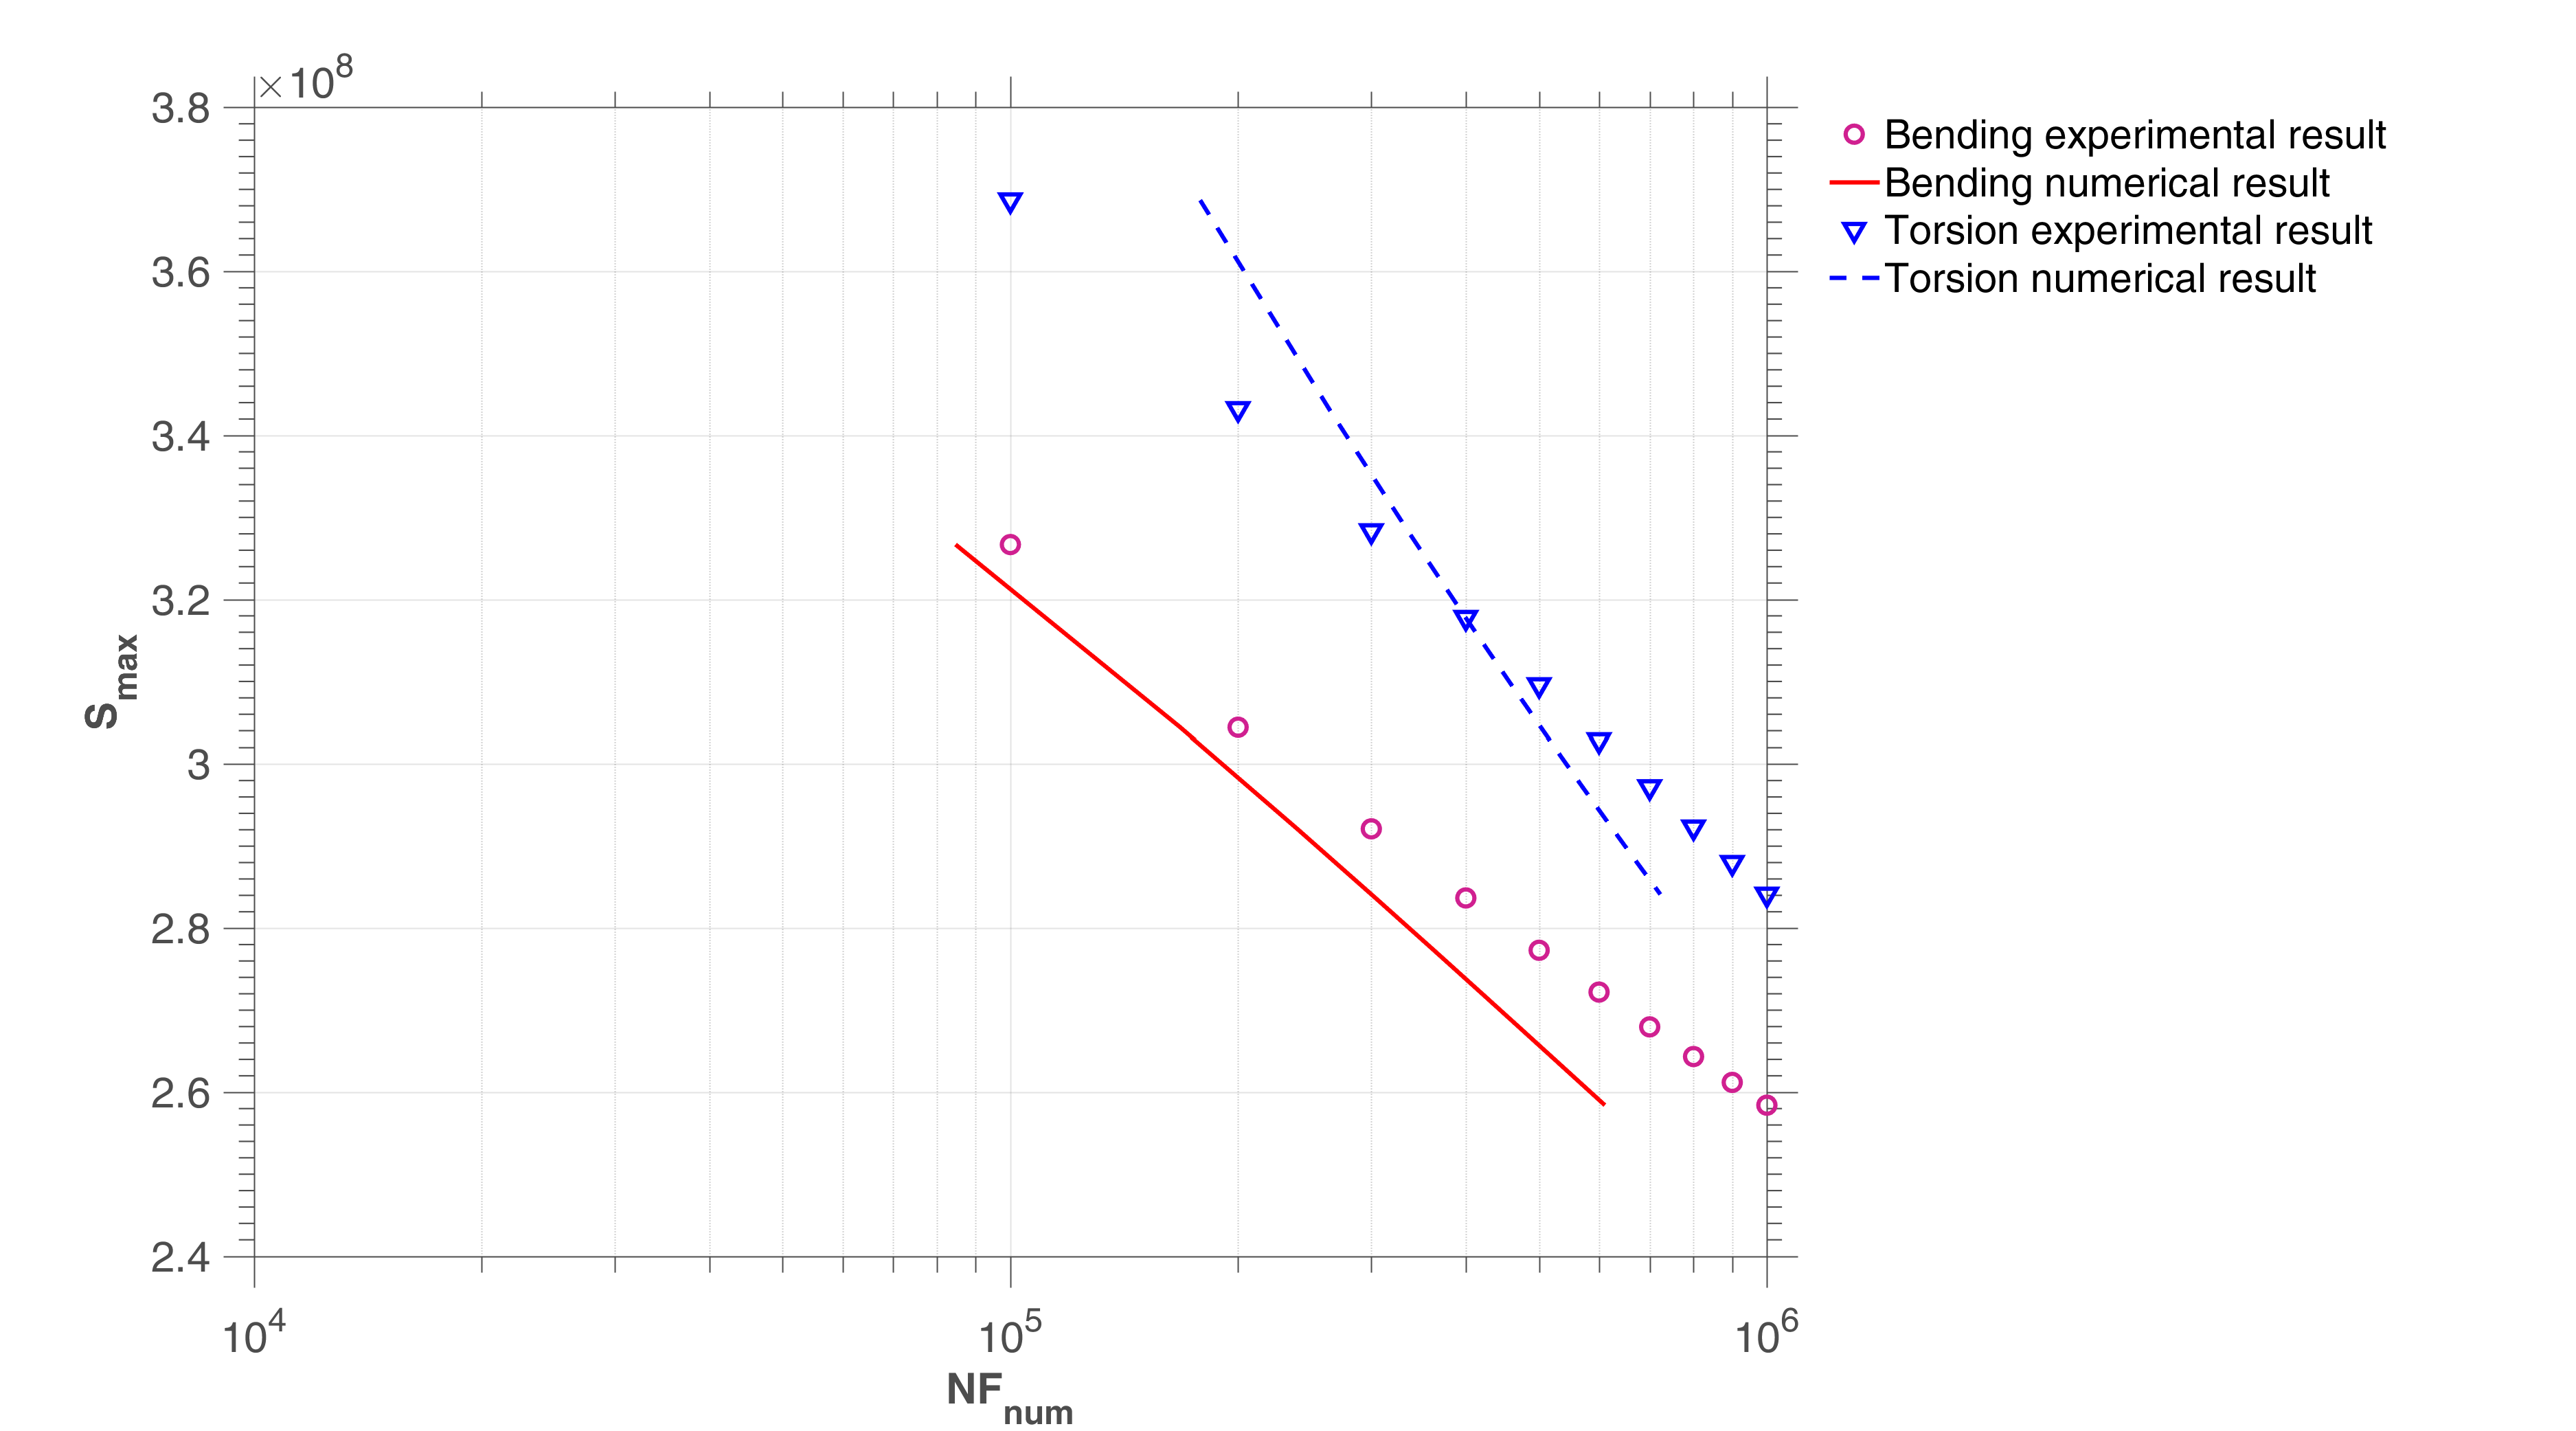
\includegraphics[width=\textwidth]{figures//bt1D_10HNAP_sn.png} 
	\caption{Bending and torsion test on 10HNAP steel(R=-1)}
	\label{fig.bt1D10HNAPsn}
\end{figure}
\begin{figure}[!h]
	\centering
	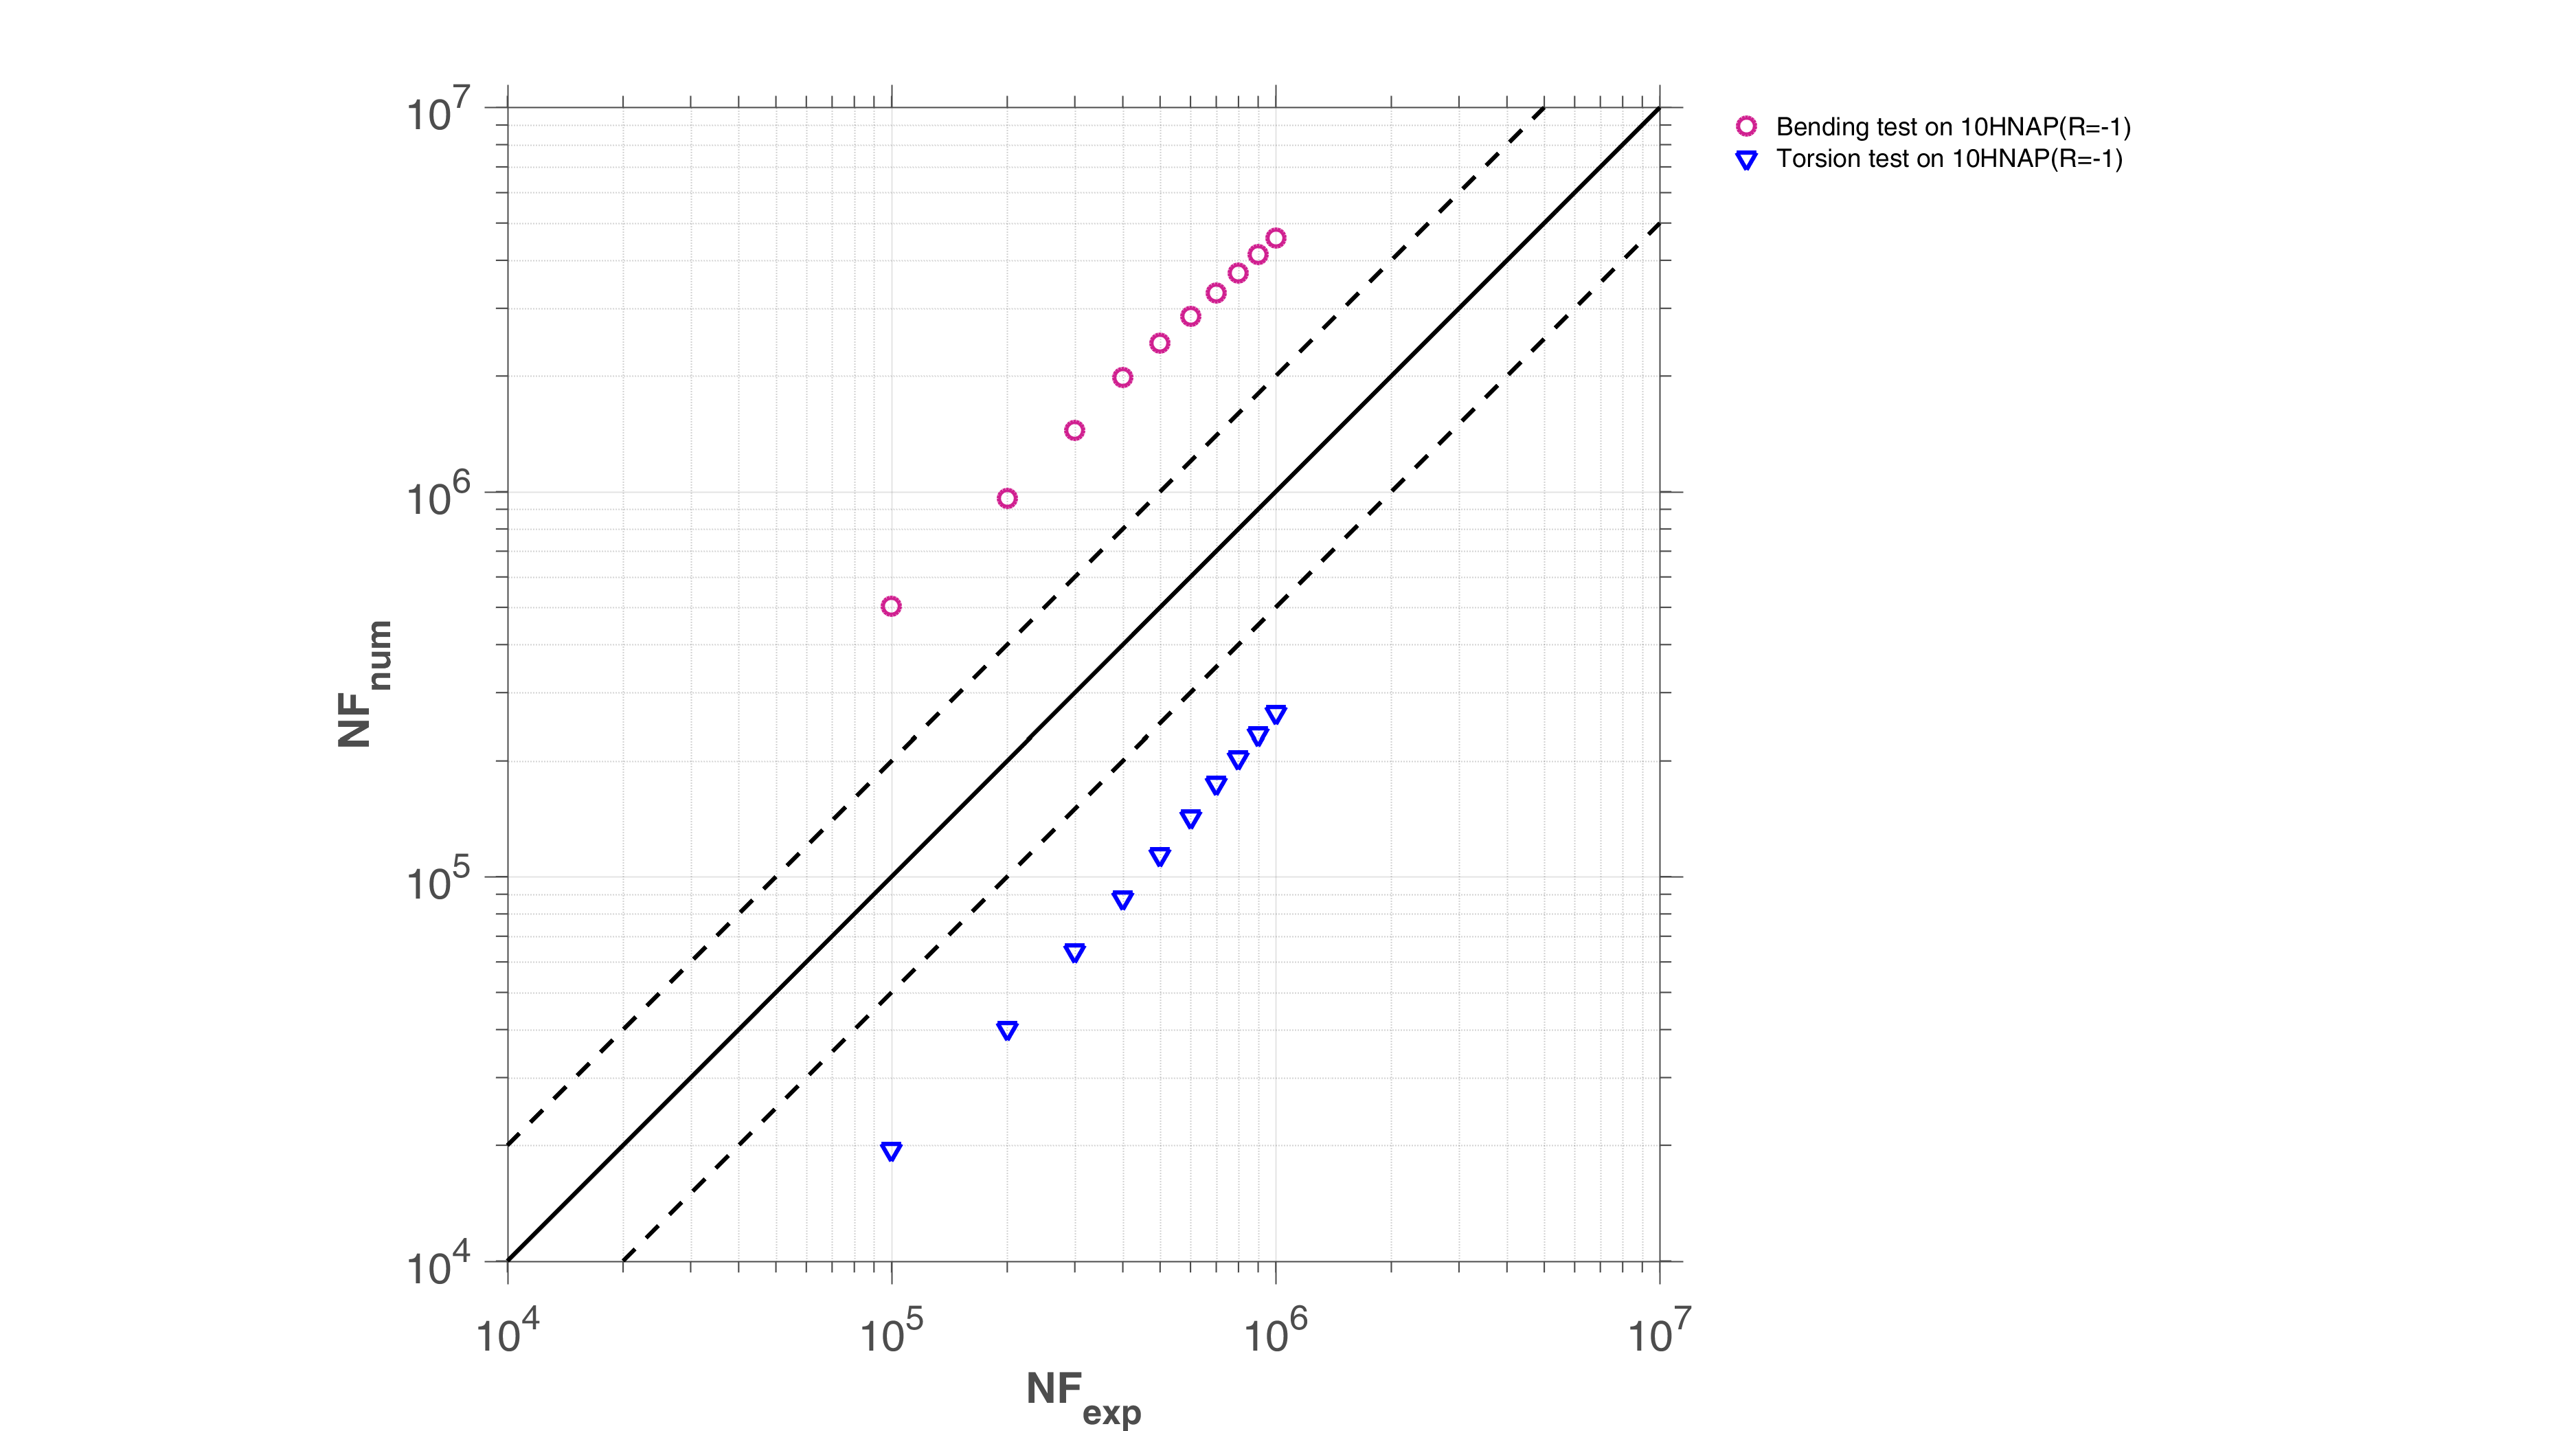
\includegraphics[width=\textwidth]{figures//bt1D_10HNAP_err1.png} 
	\caption{Bending and torsion test on 10HNAP steel(R=-1)}
	\label{fig.bt1D10HNAPerr1}
\end{figure}

The tensile Wöhler curves for various values of the mean stress are given in \figref{fig.b1Dm10HNAPsn}.


\begin{figure}[!h]
	\centering
	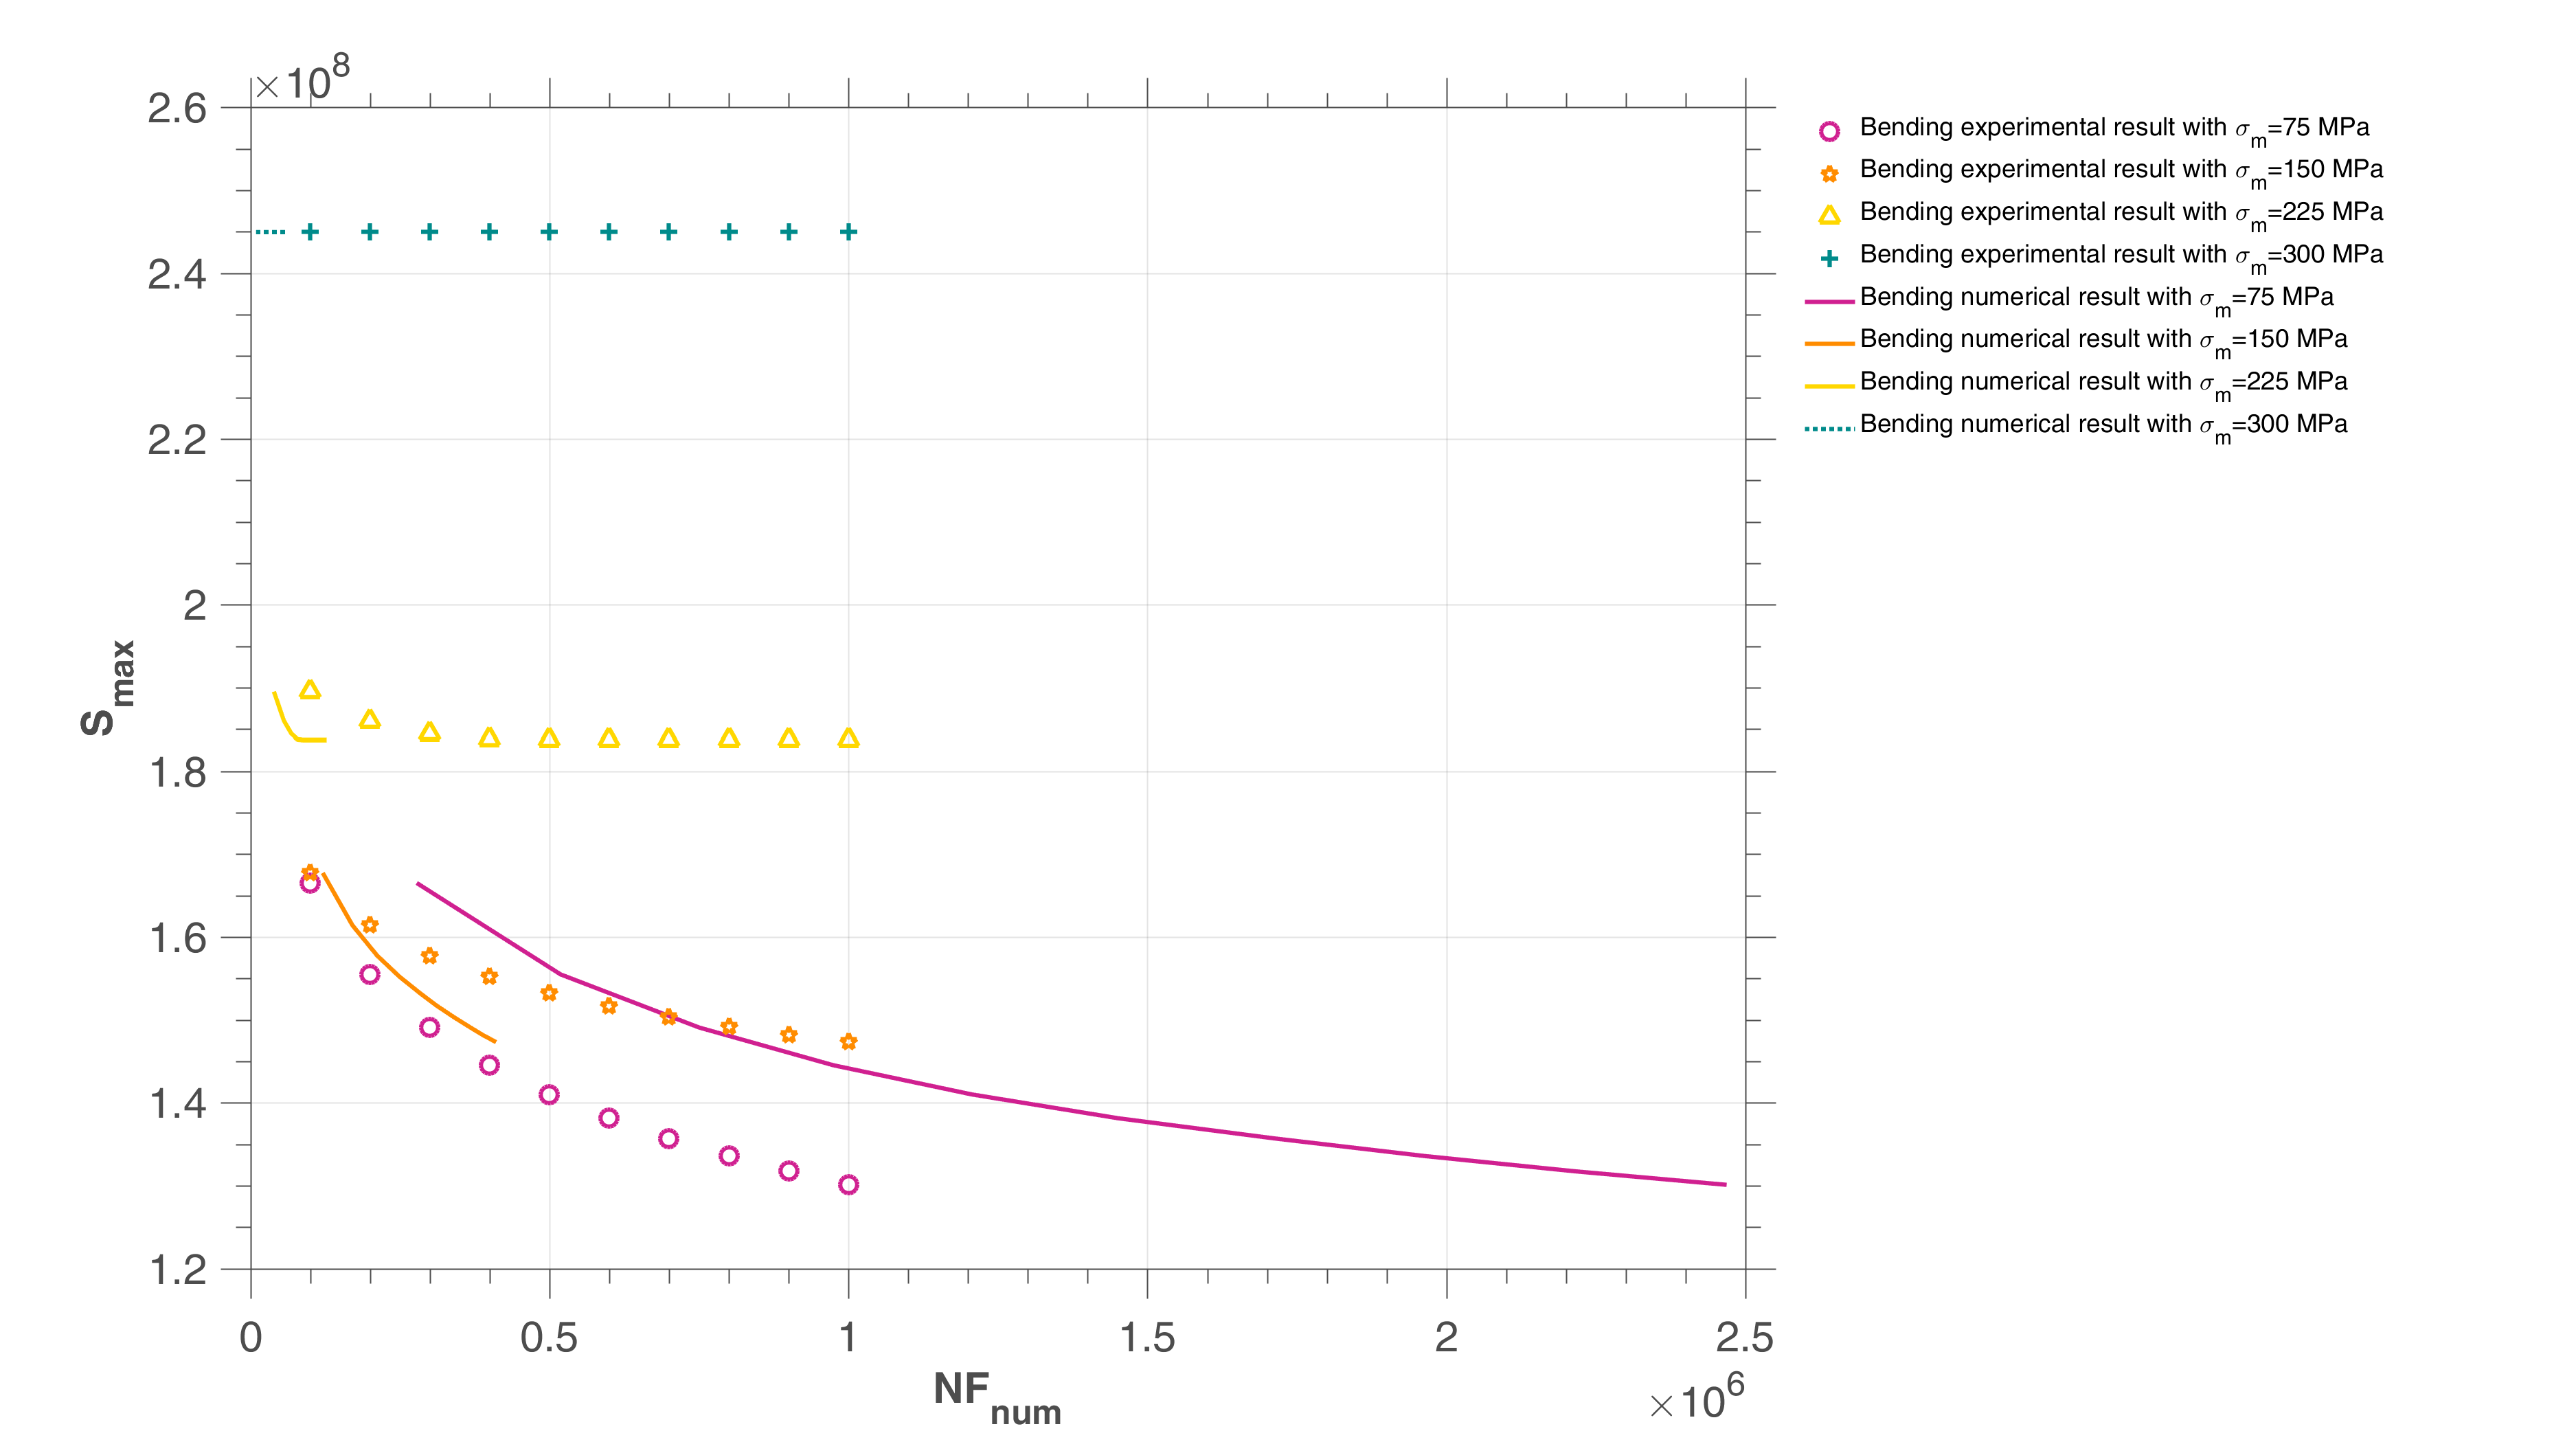
\includegraphics[width=\textwidth]{figures//b1D_m_10HNAP_sn.png} 
	\caption{Wöhler tensile curves for various mean stress values}
	\label{fig.b1Dm10HNAPsn}
\end{figure}
The prediction results of the tensile tests for various values of the mean stress σm are summarized in \figref{fig.b1Dm10HNAPerr1}. These results correlate well with the experimental lifetimes. 
\begin{figure}[!h]
	\centering
	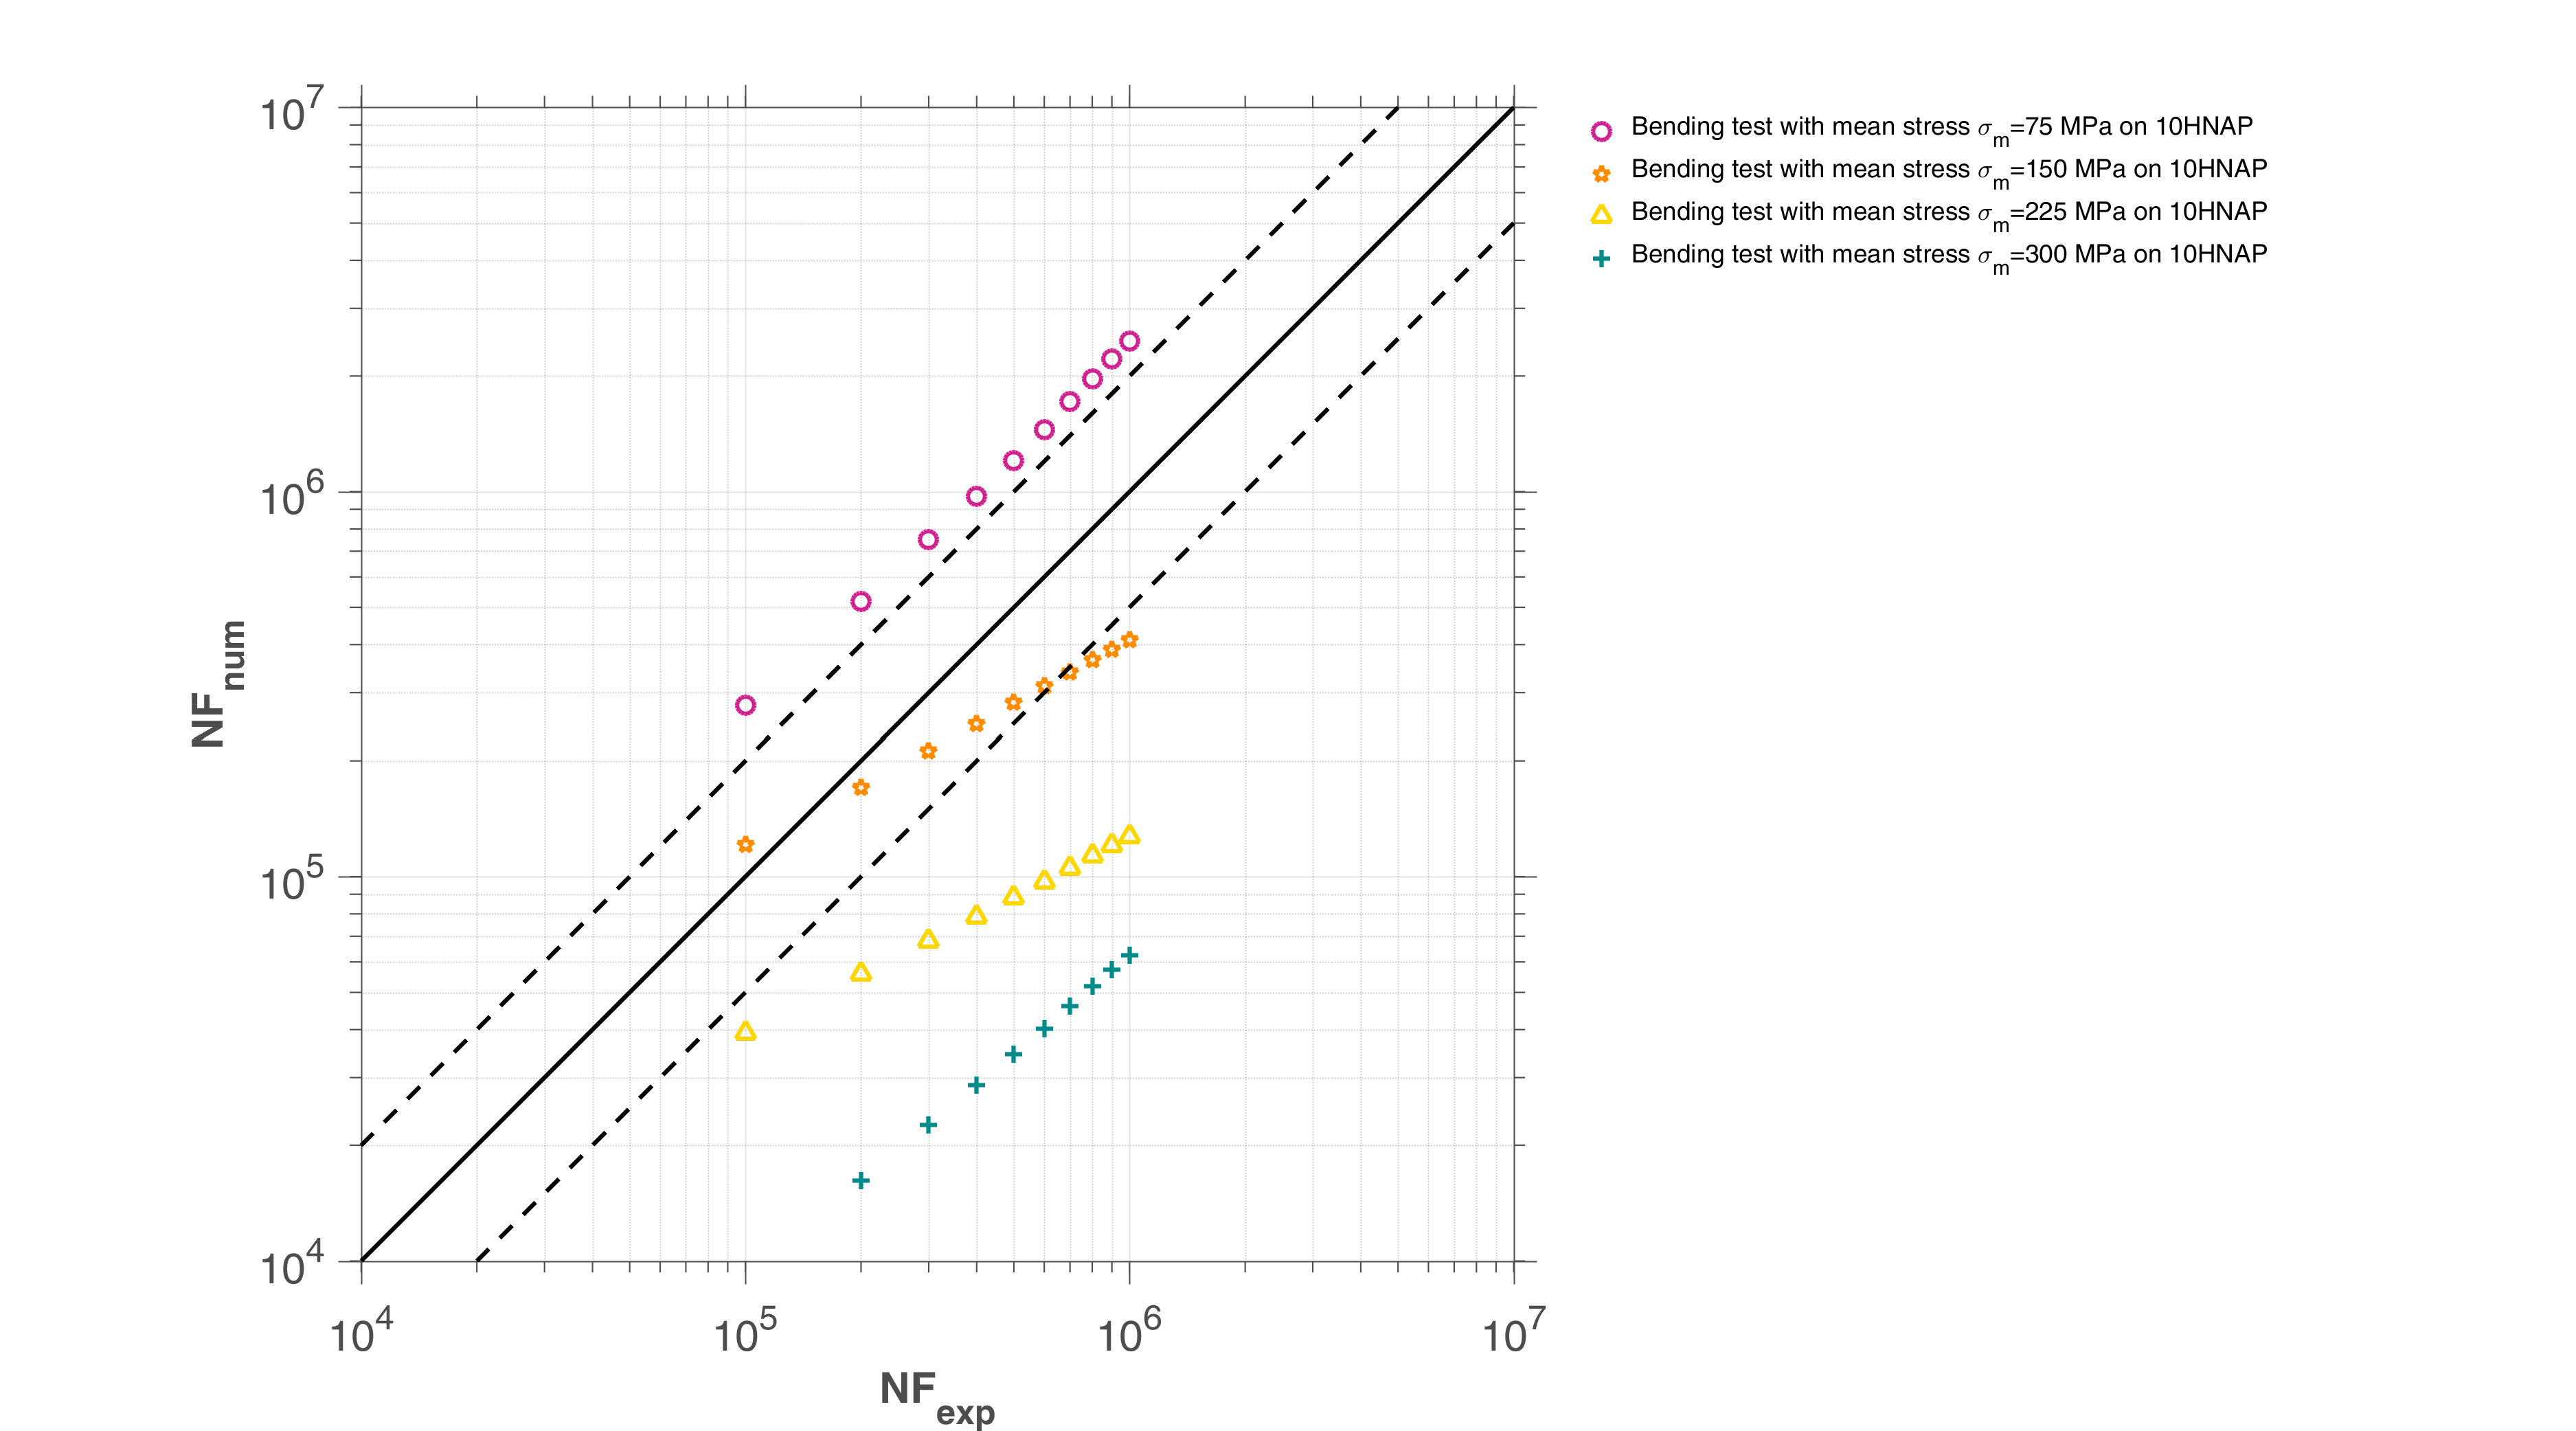
\includegraphics[width=\textwidth]{figures//b1D_m_10HNAP_err1.png} 
	\caption{Wöhler tensile curves for various mean stress values}
	\label{fig.b1Dm10HNAPerr1}
\end{figure}
The tests of multiaxial loadings of variable amplitude are plotted in Figures (3.27) and (3.28) as a function of the angle α and the ratio r. In these figures, the prediction results of the proposed model and that presented by Carpinteri et al. [17]. For the first type of tests (α = π / 8 and r = 0.2), the best predictions are given by the proposed model.
However, for the second type of tests (α = π / 4 and r = 0.5), the predictions of Carpenteri et al. [17] are relatively better.

FIG. 3.27

FIG. 3.28



\begin{comment}
\newpage
\subsection{1D data from PSA}
In this test, we reconstruct a unidimensional macroscopic stress history from recorded force data proposed by PSA group. 
\begin{figure}[!h]
	\centering
	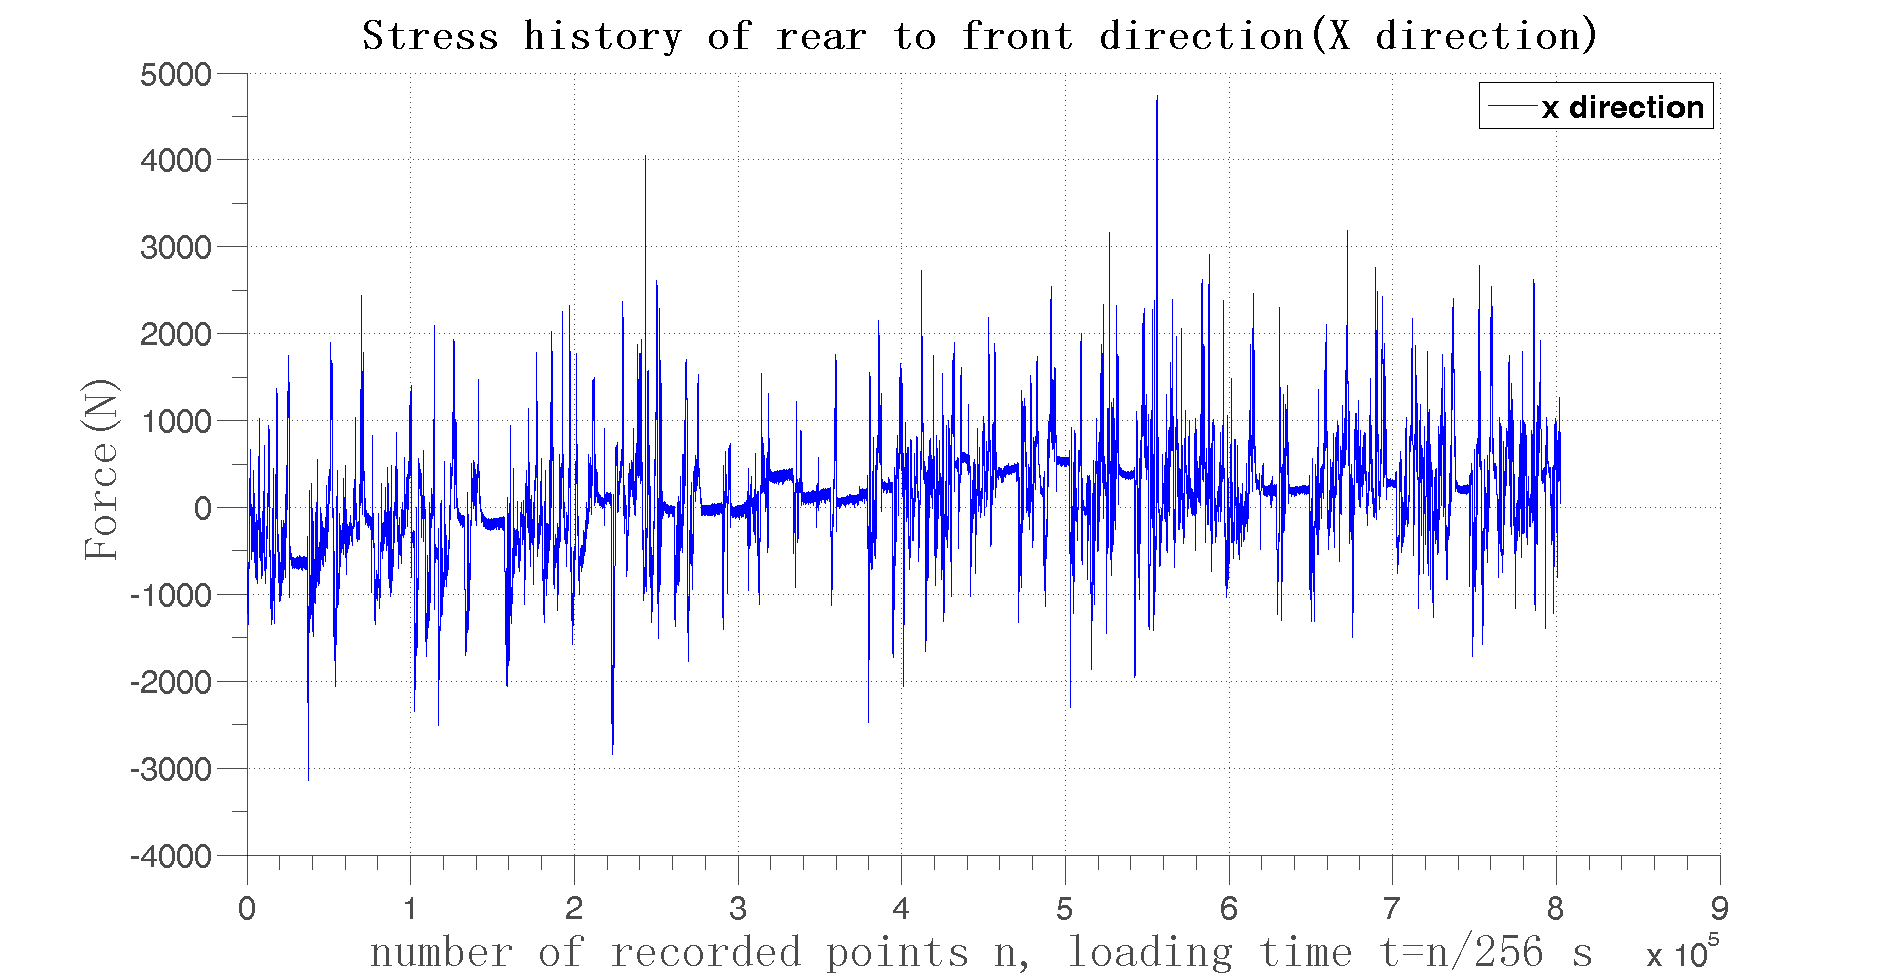
\includegraphics[width=\textwidth]{figures//x.png} 
	\caption{Loading history of X direction, force vs the record index n, with 256 sample recorded per second}
	\label{x}
\end{figure}

The force on wheel is firstly considered as under uniaxial loading $F_x$. Here we temporally set $\Sigma_x=F_x/A$ where $A=\dfrac{1}{1e6} m^2$ is the area of force, and $W_0=3e6 J$. The other data are as Table.\ref{Sin}. The plot of $\left\|  \uline{\uline{S}}-\uline{\uline{b}}\right\|_{trial}$ and $\left\|  \uline{\uline{S}}-\uline{\uline{b}}\right\|$ at 2 different scales are shown in \figref{trialreal}. The damage evolves like \figref{damage1d}. 

\begin{figure}[!h]
	\centering
	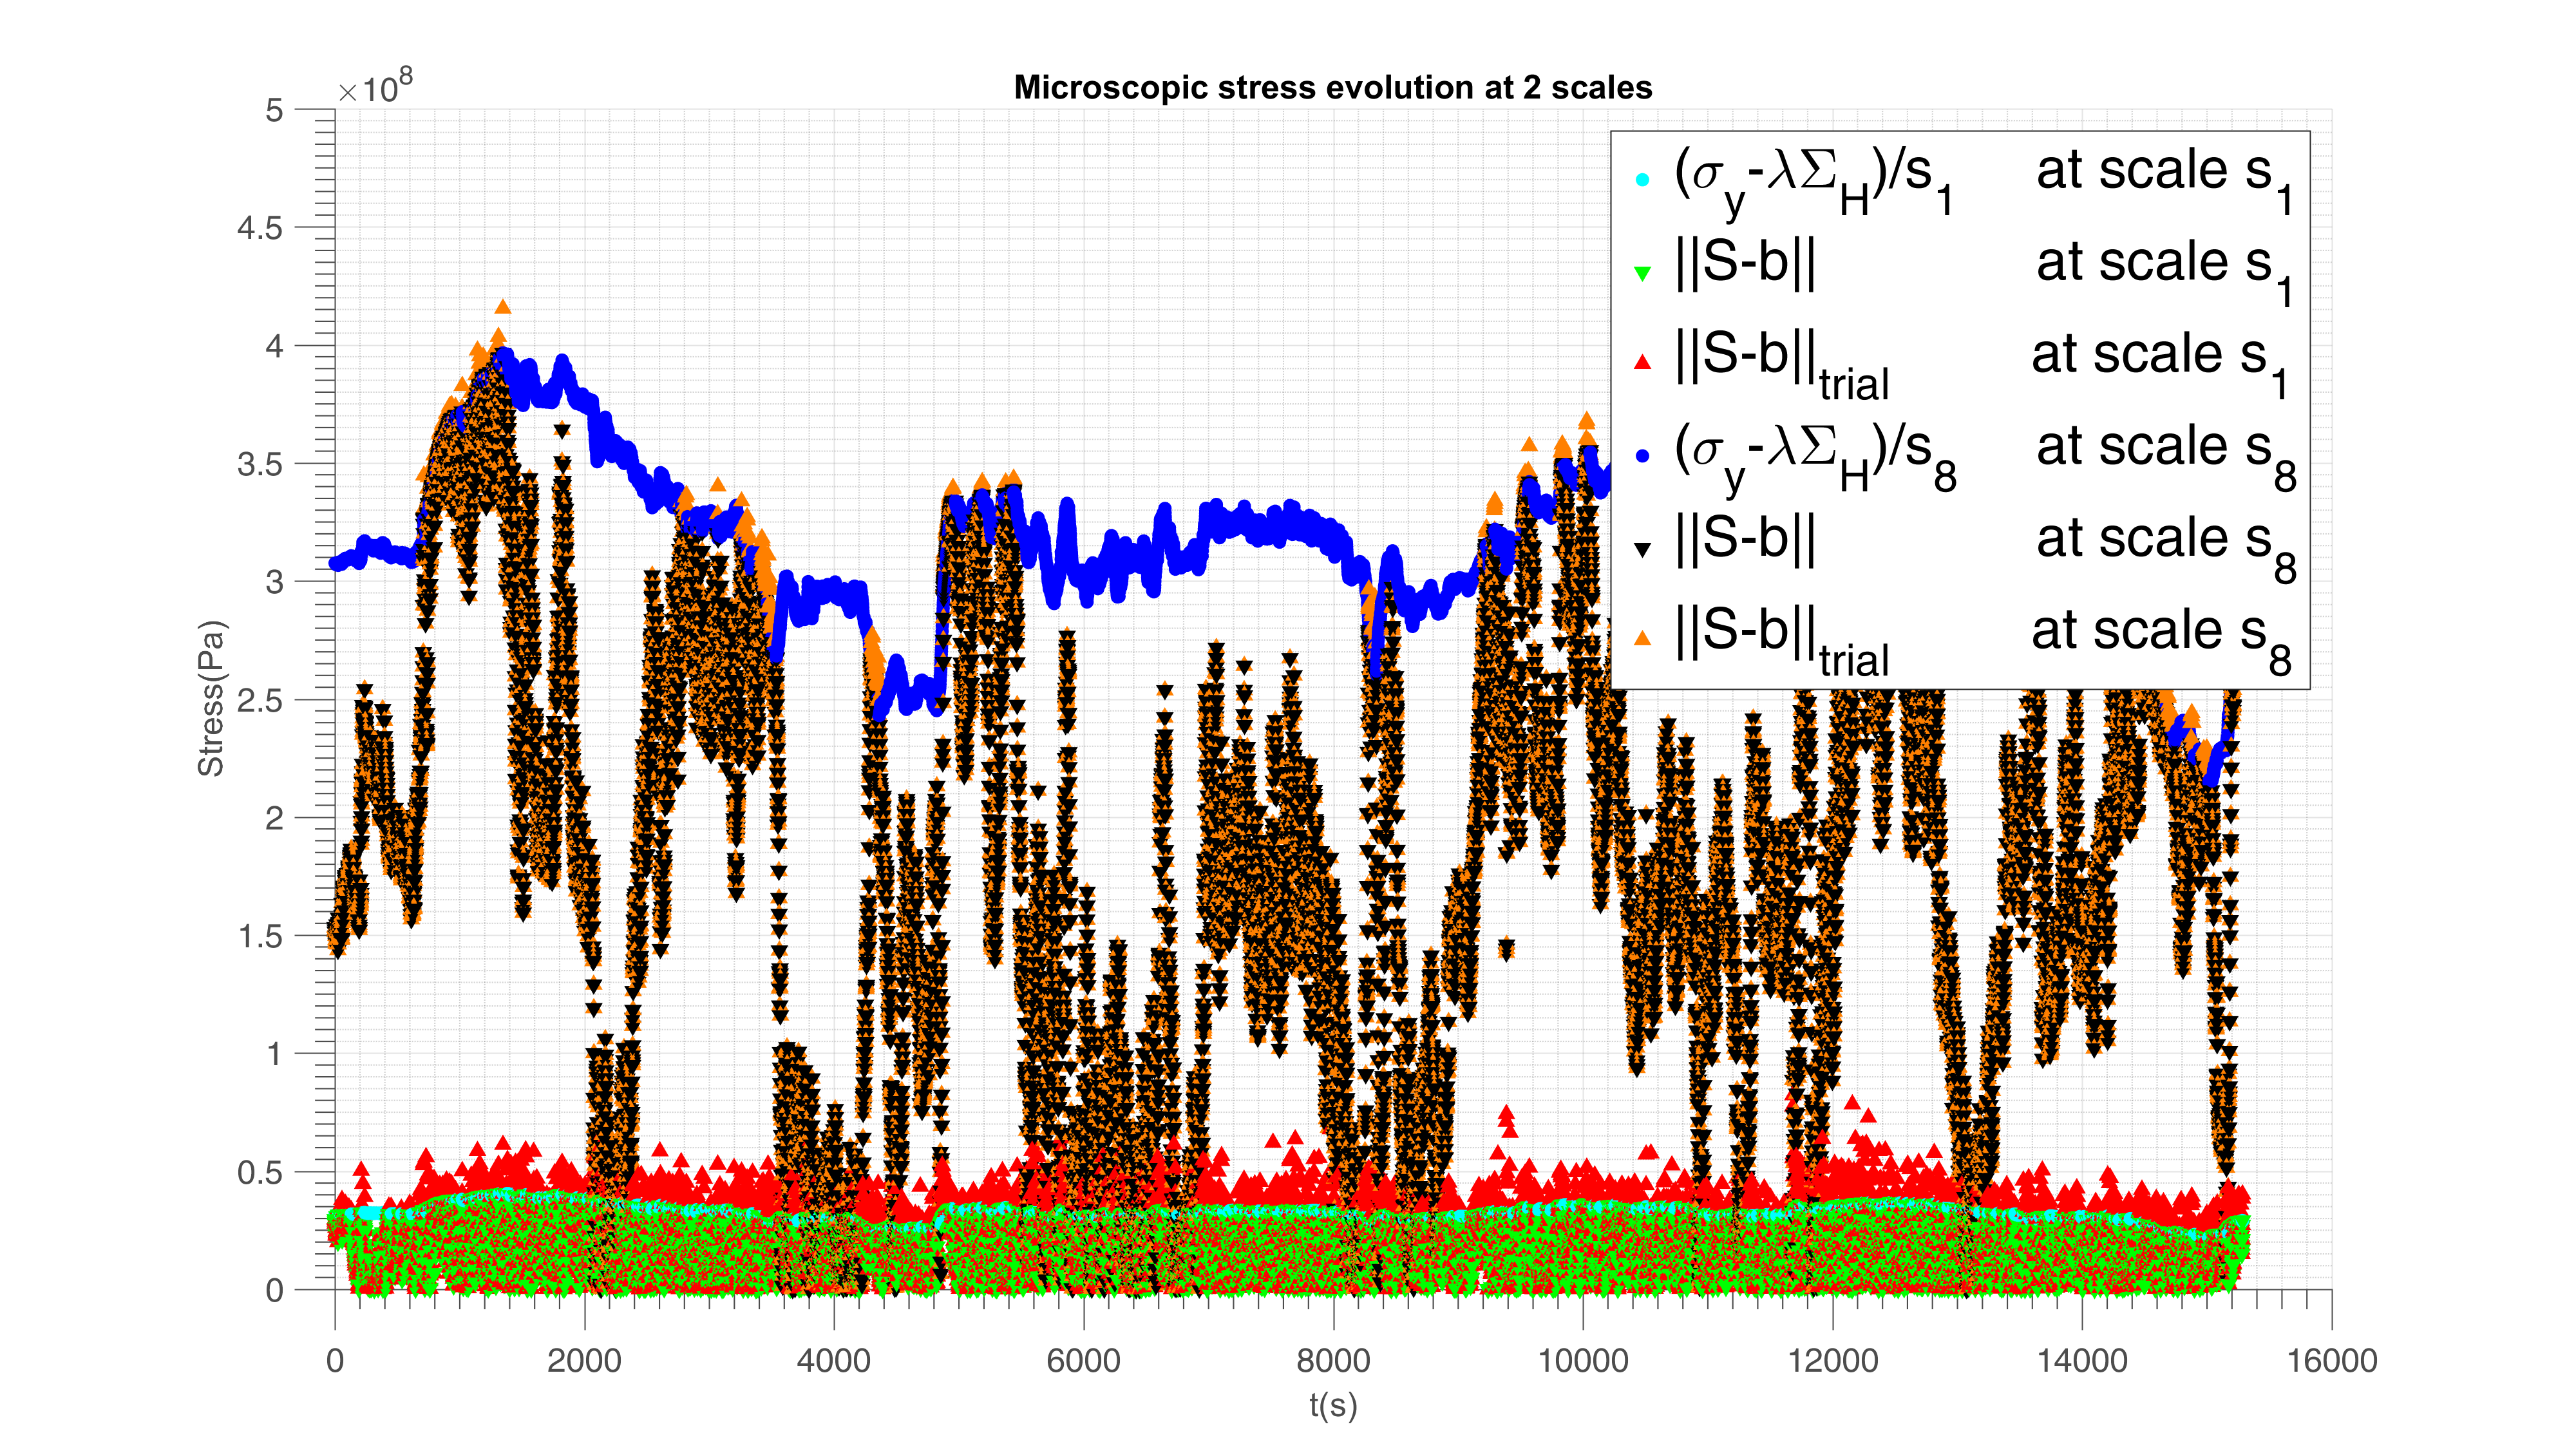
\includegraphics[width=\textwidth]{figures//trialreal1d1.png} 
	\caption{$\left\|  \uline{\uline{S}}-\uline{\uline{b}}\right\|_{trial}$ and $\left\|  \uline{\uline{S}}-\uline{\uline{b}}\right\|$ evolution with time under different weakening scales in PSA load history}
	\label{trialreal}
\end{figure}
\begin{figure}[!h]
	\centering
	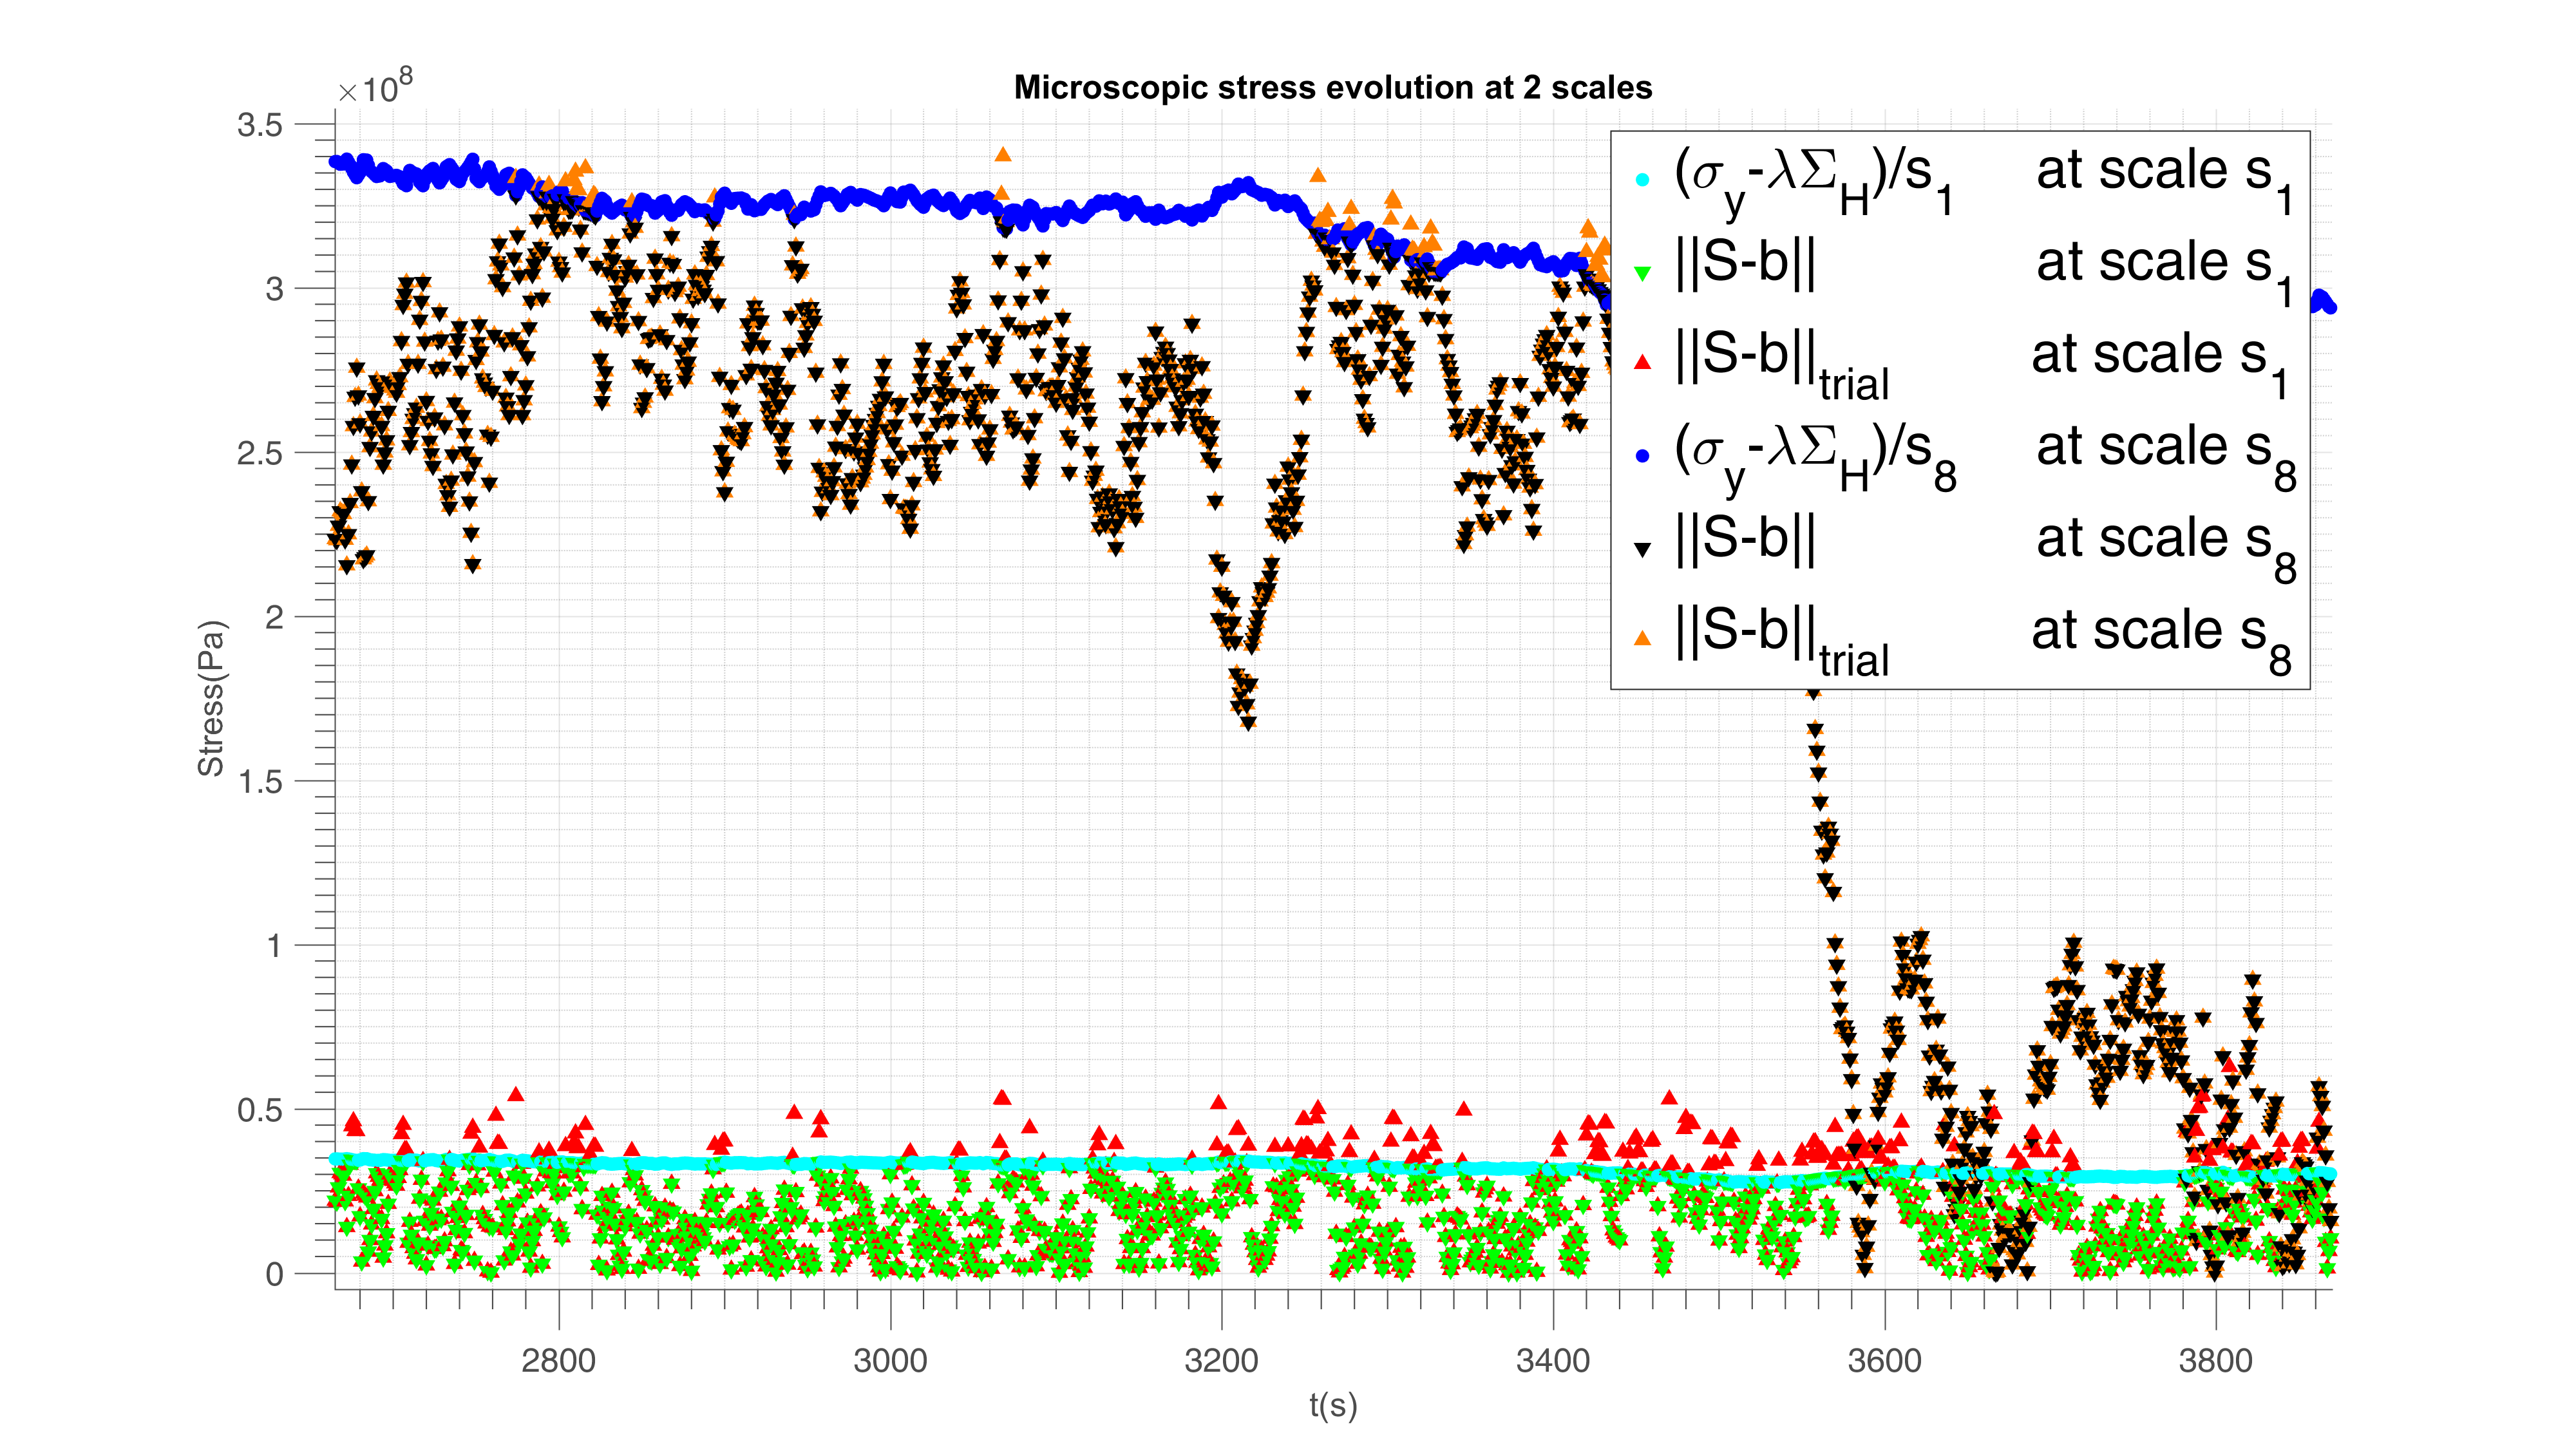
\includegraphics[width=\textwidth]{figures//trialreal1d2.png} 
	\caption{Circled area magnification in \figref{trialreal} where there is more $\left\|  \uline{\uline{S}}-\uline{\uline{b}}\right\|_{trial}>\left(\sigma_y-\lambda \Sigma_H\right)$(plasticity)  at $s_1$ than at $s_8$}
	\label{trialreal1d2}
\end{figure}
\begin{figure}[!h]
	\centering
	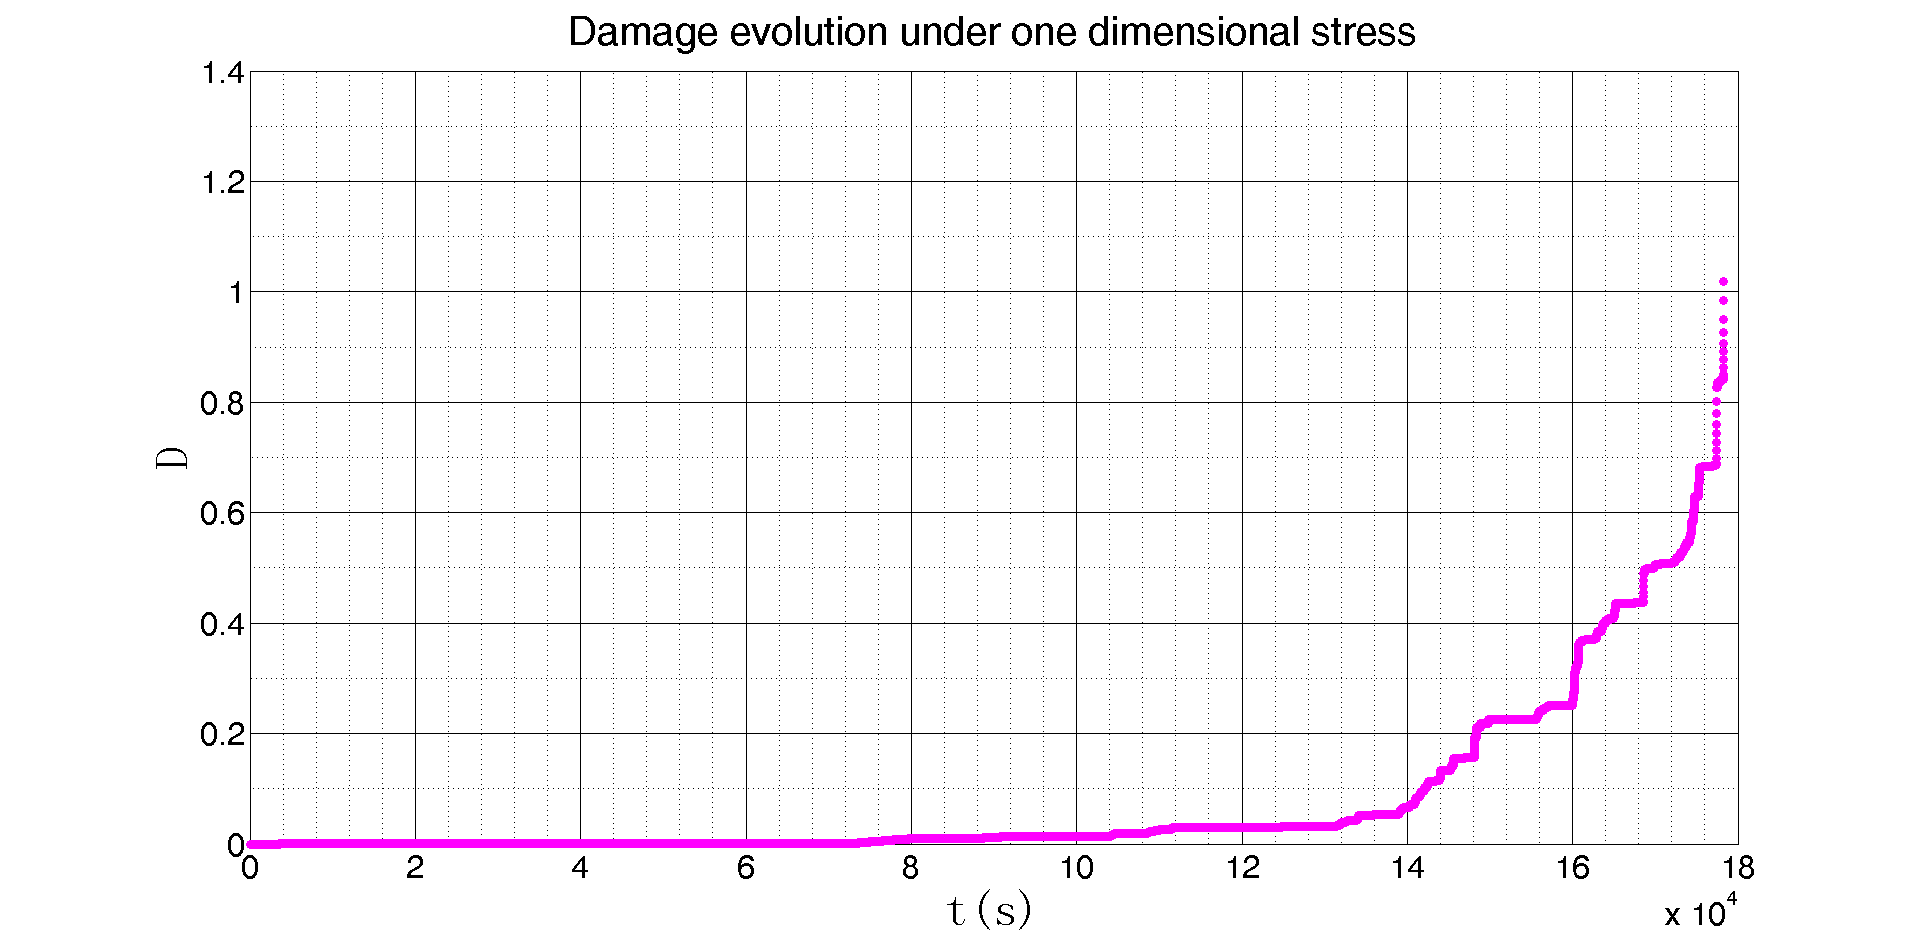
\includegraphics[width=\textwidth]{figures//damage1d.png} 
	\caption{Damage evolution with time at one dimension PSA load history}
	\label{damage1d}
\end{figure}

 \newpage
 \subsection{Multi-dimensional application to PSA data}
 We now consider a situation where we have force recorded measured in 3 different directions as shown in \figref{xyz}.
 \begin{figure}[!h]
 	\centering
 	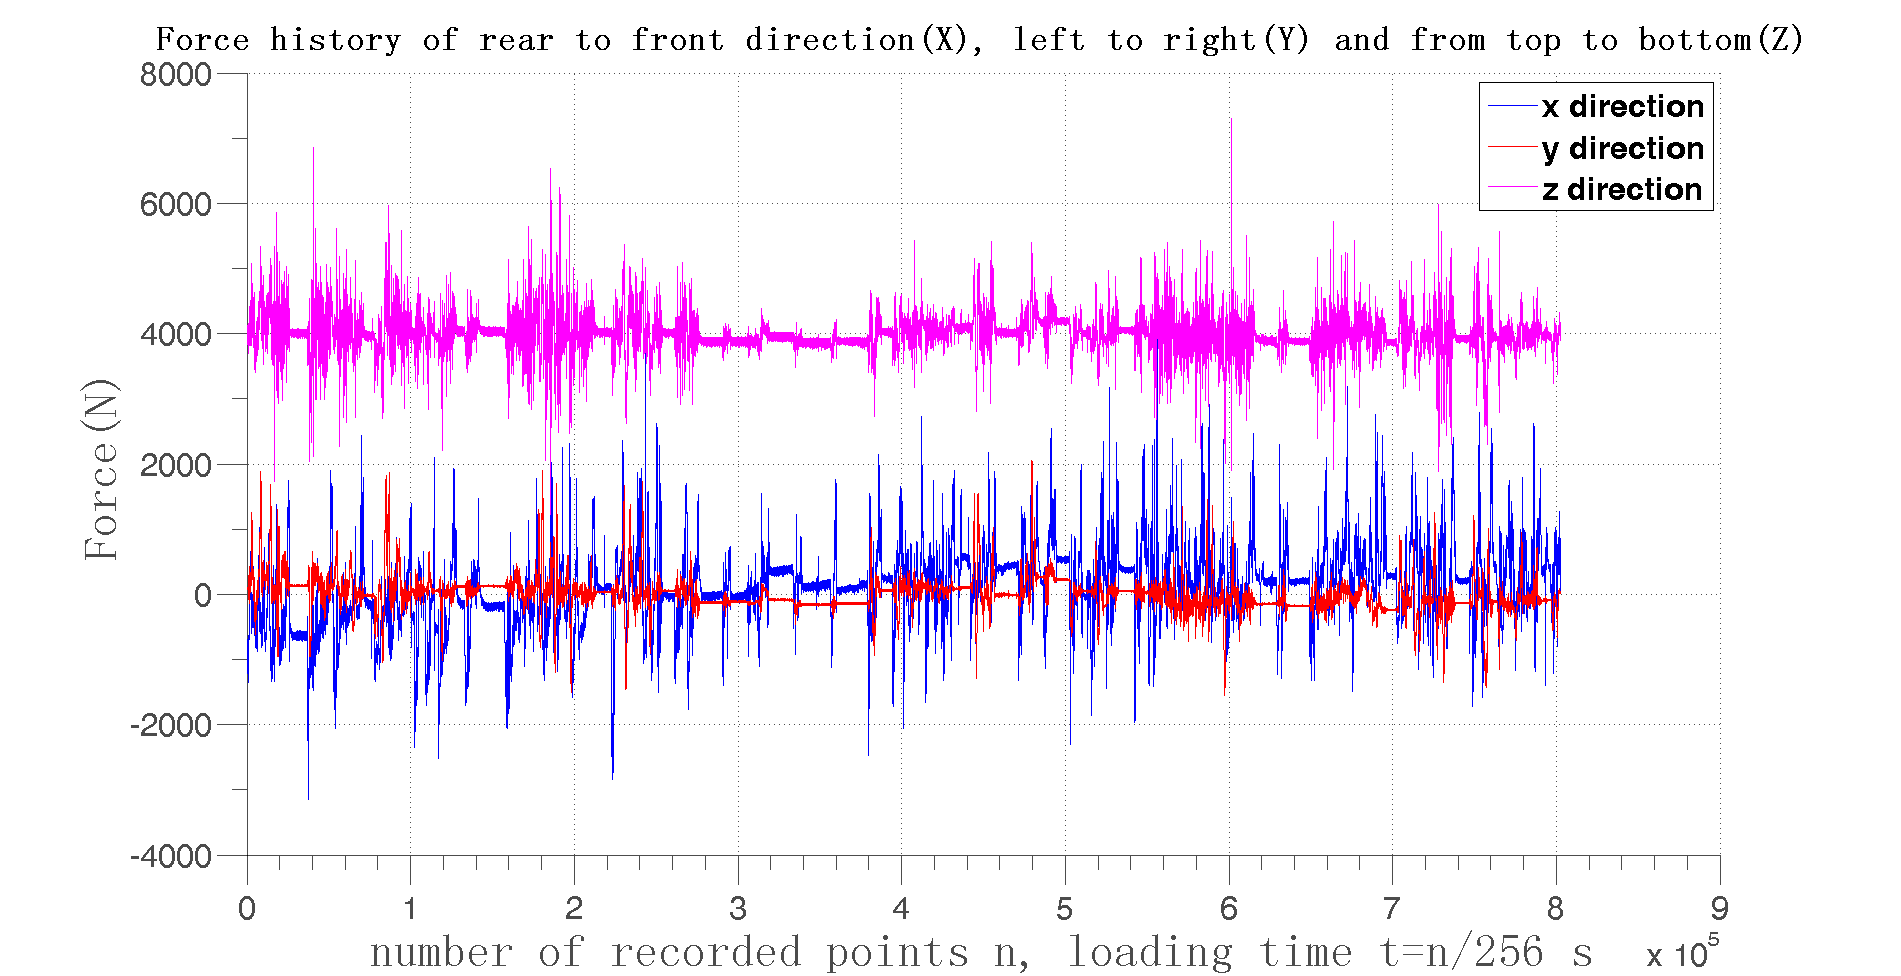
\includegraphics[width=\textwidth]{figures//xyz.png} 
 	\caption{Loading history of 3 different directions}
 	\label{xyz}
 \end{figure}
  \begin{figure}[!h]
  	\centering
  	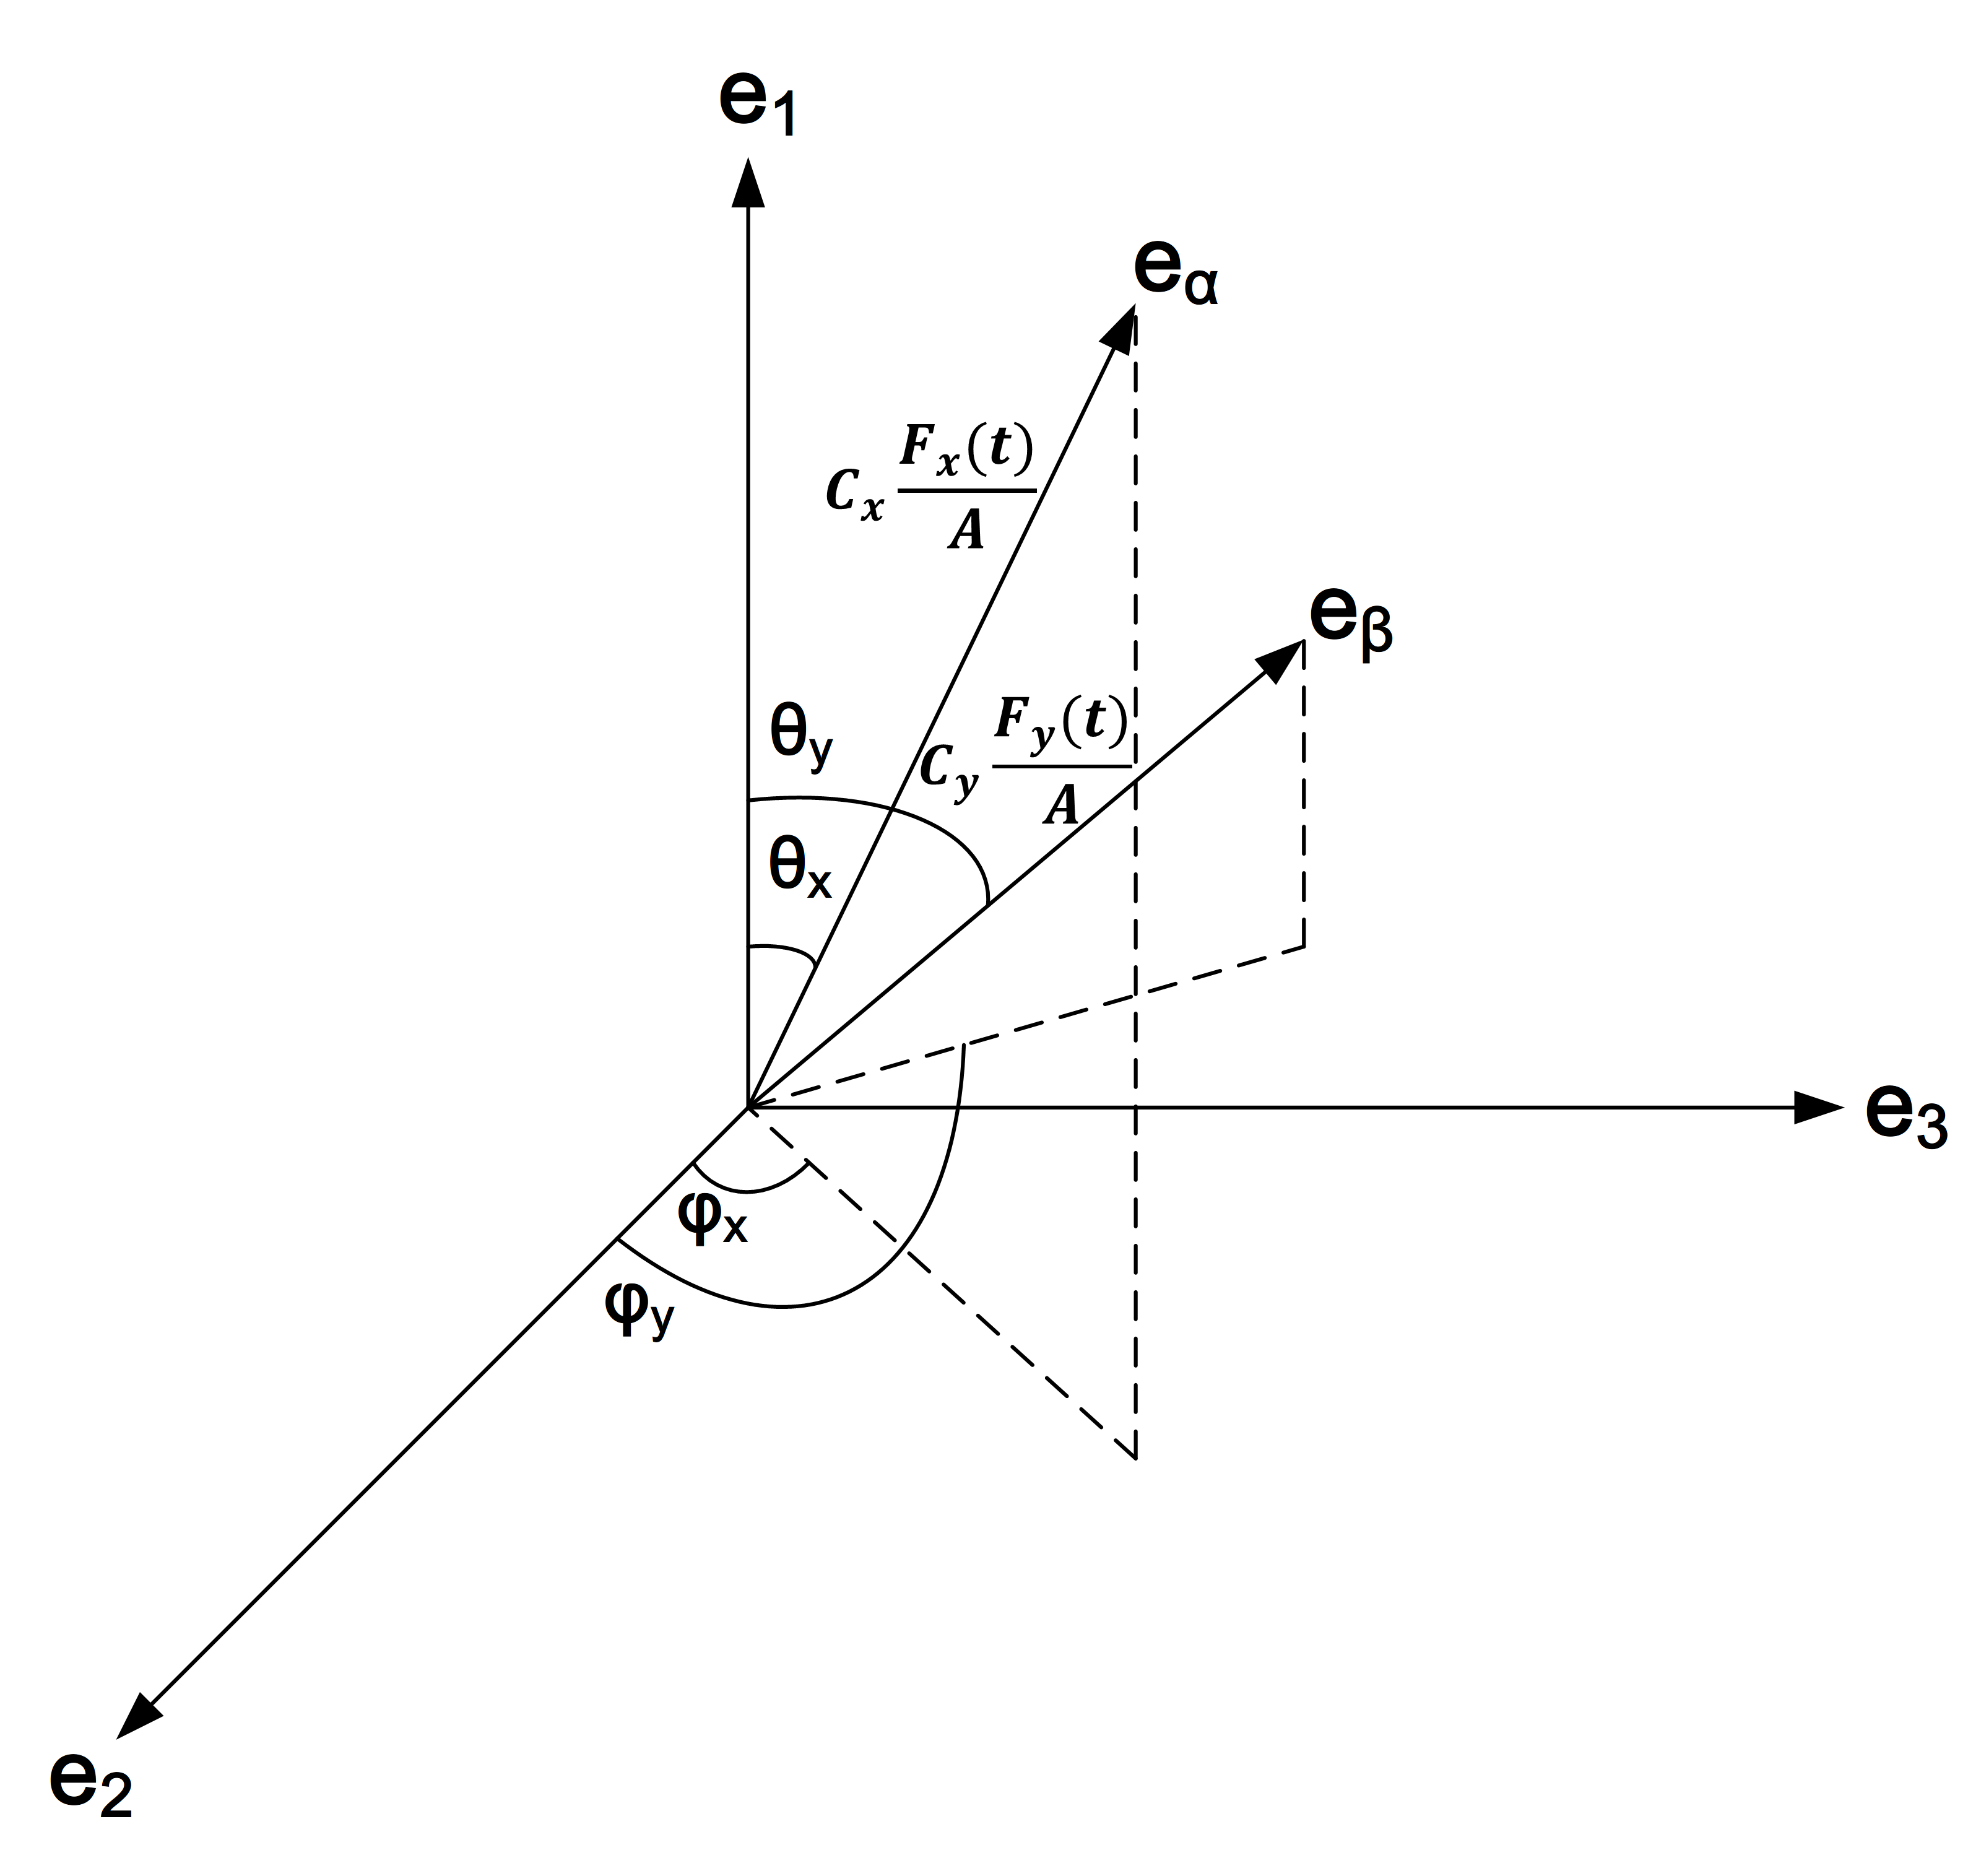
\includegraphics[width=0.7\textwidth]{figures//xab.png} 
  	\caption{Loading in 3 different directions}
  	\label{xab}
  \end{figure}
 In real case, the vertical force $F_z$ is much larger than the axial and horizontal forces $F_x$ and $F_y$, as shown in \figref{xyz}. However, in order to investigate large domains of interest, we first scale the axial and horizontal forces to reach comparable impact and transform them in principal stresses $c_x\dfrac{F_x}{A}$ applied along the stress principle vector $\uline{e}_\alpha$(respectively $\uline{e}_\beta$) that we choose randomly(\figref{xab}). We therefore consider the following macroscopic stress tensor:
 \begin{equation}
 \uline{\uline{\Sigma}}=\dfrac{F_z(t)}{A}\uline{e}_1\otimes \uline{e}_1+c_x\dfrac{F_x(t)}{A}\uline{e}_{\alpha}\otimes \uline{e}_{\alpha}+c_y\dfrac{F_y(t)}{A}\uline{e}_{\beta}\otimes \uline{e}_{\beta}
 \label{tensor1}
 \end{equation}
 where $\uline{e}_{\alpha}$  and $\uline{e}_{\beta}$ are principal vectors whose spherical coordinate are $\theta_x$, $\varphi_x$,  $\theta_y$ and $\varphi_y$ respectively:
  $$\uline{e}_{\alpha}=cos\theta_x\uline{e}_1+sin\theta_xcos\varphi_x\uline{e}_2+sin\theta_xsin\varphi_x\uline{e}_3,$$
 $$\uline{e}_{\beta}=cos\theta_y\uline{e}_1+sin\theta_ycos\varphi_y\uline{e}_2+sin\theta_ysin\varphi_y\uline{e}_3.$$
 Here $F_x(t)$, $F_y(t)$, $F_z(t)$ are from test data, and $\theta_x$, $\varphi_x$, $\theta_y$, $\varphi_y$ are structural parameters to be chosen randomly.The physical data are the same with parameters in Table.\ref{Sin}. The structural data we choose is shown in Table.\ref{structural}.
 
  \begin{table}[!h]
  	\centering
    \begin{tabular}{rrrrrrrr}
  		\hline
  		\textbf{Parameter} & A($m^2$) & $c_x$ & $c_y$ & $\theta_x$ & $\varphi_x$ & $\theta_y$ & $\varphi_y$ \\
  		\textbf{Value}      & 1/6e4                  & 10    & 60    & 0.5        & 0.3         & 0.6        & 0.4         \\ \hline
  	\end{tabular}
  	\caption{The structural data in 3D analysis}
  	\label{structural}
  \end{table}
 
 The underlying assumption is that a unit load on wheel in direction $\uline{e}_x$ creates a stress tensor at point $M$ given by:
 $$c_x\dfrac{F_x(t)}{A}\uline{e}_{\alpha}\otimes \uline{e}_{\alpha},$$
 where $\uline{e}_{\alpha}\otimes \uline{e}_{\alpha}$ defines the local structural response of the vehicle.
 
 Replacing $\uline{e}_{\alpha}$ and $\uline{e}_{\beta}$ in Eq.\eqref{tensor1} we get the stress tensor in Eq.\eqref{tensor2} in the annex. 
  
 The plot of $\left\|  \uline{\uline{S}}-\uline{\uline{b}}\right\|_{trial}$ and $\left\|  \uline{\uline{S}}-\uline{\uline{b}}\right\|$ under 2 different scales are shown in \figref{trialreal3d}.
\begin{figure}[!h]
	\centering
	\includegraphics[width=\textwidth]{figures//trialreal3d.png} 
	\caption{$\left\|  \uline{\uline{S}}-\uline{\uline{b}}\right\|_{trial}$ and $\left\|  \uline{\uline{S}}-\uline{\uline{b}}\right\|$ evolution with time under different weakening scales in PSA load history}
	\label{trialreal3d}
\end{figure} 

In the load history, when $\left\|  \uline{\uline{S}}-\uline{\uline{b}}\right\|_{trial}>\left(\sigma_y-\lambda \Sigma_H\right)$, the damage accumulates. However, at scale $s_{8}$, there are much less damage accumulation than at scale $s_1$.  In this way we do not neglect the small influences in load history and the big fluctuation in stress is magnified which reflects the real situation. 


The damage evolves like in \figref{dam3d}. 


\begin{figure}[!h]
	\centering
	\includegraphics[width=\textwidth]{figures//damage3d.png} 
	\caption{Damage evolution under multidimensional stress}
	\label{dam3d}
\end{figure}

\end{comment}

\clearpage
\section{Discussion}
We work on the stress tensor directly in 3D analysis in stead of using the multidimensional equivalent stress.
The strategy can be made more complex by introducing a local space averaging process in the calculation of the local damage, and by taking more general plastic flows. The energy based fatigue approach takes into account impurities and hardness in the material and is applicable to any type of micro plasticity law and multiaxial load geometry. The time implicit strategy gets rid of cycle counting which is hardly applicable to complex loading, big fluctuation is magnified which reflects the real situation.

The advantages and drawbacks of our proposed model are listed as follows:
\begin{enumerate}
	\vspace{6pt}
	\item No rain-flow filter
	
	\vspace{6pt}
	\item
	No cycle counting
	
	\vspace{6pt}
	\item
	Possible handling of different SN curves.
	
	\vspace{6pt}
	\item
	Random loading suitability with nonlinear damage accumulation
	
	
	\vspace{6pt}
	\item
	{\textcolor{blue} {Requires a scale by scale analysis}}
	
	\vspace{6pt}
	\item
	Real multi-axial tests to be applied.
	
\end{enumerate}

\vspace{6pt}
\noindent
\textbf{Acknowledgments}

\vspace{6pt}
We are grateful for the financial and technical support of Chaire PSA.

\bibliographystyle{unsrt}
\bibliography{11}
\addcontentsline{toc}{section}{Reference}



\clearpage
\appendix
\appendixpage
\addcontentsline{toc}{section}{Appendices}\markboth{APPENDICES}{}
\lstset{% general command to set parameter(s)
	basicstyle=\small, % 设置字体大小
	keywordstyle=\color{red}, % 设置关键字格式(颜色等等)
	identifierstyle=, % nothing happens
	commentstyle=\color{blue}, % 设置注释的格式
	stringstyle=\ttfamily, % typewriter type for strings
	showstringspaces=false} % no special string spaces
	\section{DETAILED EXPLOITATION}
	************************************************************************************

 A DETAILED DESCRIPTION OF ANALYTICAL EXPLOITATION ON UNIAXIAL CYCLE
 
\noindent              
************************************************************************************

\noindent
\textbf{Phase 1:} The deviatoric stress amplitude increases from $\sigma_y/s$ to $S_{max}$.

\noindent
The material is in local plastic regime, then $\dot{\varepsilon}^p>0$ and $\dot{\sigma}-\dot{b}=0$ $\Rightarrow$ $\dot{\Sigma}-\dfrac{E}{1+\nu}\dot{\varepsilon}^p=\dfrac{kE}{E-k}\dot{\varepsilon}^p$ $\Rightarrow$ 
$$\dot{\varepsilon}^p=\dfrac{(E- k)(1+\nu)}{E(E+k\nu)}\dot{\Sigma}.$$

\vspace{6pt}
\noindent
$\Rightarrow$ $\dot{\varepsilon}^p$ varies from 0 to $\dfrac{(E- k)(1+\nu)(S_{max}-\sigma_y/s)}{E(E+k\nu)}$.

\vspace{6pt}
\noindent
From Taylor-Lin scale transition model:
$$\dot{\sigma}=\dot{\Sigma}-\dfrac{E}{1+\nu}\dot{\varepsilon}_p=\dot{\Sigma}-\dfrac{E-k}{E-\nu k}\dot{\Sigma}=\dfrac{k(1-\nu)}{E-k\nu}\dot{\Sigma}.$$

\vspace{6pt}
\noindent
$\Rightarrow$ $\sigma$ varies from $\sigma_y/s$ to $\sigma_y/s+\dfrac{k(1-\nu)(S_{max}-\sigma_y/s)}{E-k\nu}$.

\vspace{6pt}
$$\dot{b}=\dot{\Sigma}-\dfrac{E}{1+\nu}\dot{\varepsilon}_p=\dot{\Sigma}-\dfrac{E-k}{E-\nu k}\dot{\Sigma}=\dfrac{k(1-\nu)}{E-k\nu}\dot{\Sigma}.$$

\vspace{6pt}
\noindent
$\Rightarrow$ $b$ varies from $0$ to $\dfrac{k(1-\nu)(S_{max}-\sigma_y/s)}{E-k\nu}$.

\vspace{6pt}
\noindent
So the energy dissipation rate is: $$(\sigma-b)\dot{\varepsilon}^p=\dfrac{\sigma_y}{s}\dot{\varepsilon}^p=\dfrac{\sigma_y}{s}\dfrac{(E- k)(1+\nu)}{E(E+k\nu)}\dot{\Sigma}.$$

\noindent
The energy dissipation is: $$(\sigma-b)\Delta\varepsilon^p=\dfrac{\sigma_y}{s}\dfrac{(E- k)(1+\nu)(S_{max}-\sigma_y/s)}{E(E+k\nu)}.$$

\vspace{6pt}
\noindent
\textbf{Phase 2:} The deviatoric stress amplitude decreases from $S_{max}$ to $S_{max}-2\sigma_y/s$.

\noindent
The material is in local elastic regime, then $\dot{\varepsilon}^p=0$ and $\dot{\sigma}-\dot{b}=0$ $\Rightarrow$

\vspace{6pt}
\noindent
$\dot{b}=0$, $\dot{\sigma}=\dot{\Sigma}-\dfrac{E}{1+\nu}\dot{\varepsilon}_p=\dot{\Sigma}$.

\vspace{6pt}
\noindent
$\sigma$ varies from $\sigma_y/s+\dfrac{k(1-\nu)(S_{max}-\sigma_y/s)}{E-k\nu}$ to $-\sigma_y/s+\dfrac{k(1-\nu)(S_{max}-\sigma_y/s)}{E-k\nu}$.

\vspace{6pt}
\noindent
$\sigma-b$ varies from $\sigma_y/s$ to $-\sigma_y/s$.

\vspace{6pt}
\noindent
The energy dissipation rate is: $$(\sigma-b)\dot{\varepsilon}^p=0.$$

\vspace{6pt}
\noindent
\textbf{Phase 3:} The deviatoric stress amplitude decreases from $S_{max}-2\sigma_y/s$ to $-S_{max}$.

\noindent
The material is in local plastic regime, then $\dot{\varepsilon}^p>0$ and $\dot{\sigma}-\dot{b}=0$ $\Rightarrow$ 
$$\dot{\varepsilon}^p=\dfrac{(E- k)(1+\nu)}{E(E+k\nu)}\dot{\Sigma}$$ as opposite to phase 1 for $\dot{\Sigma}<0$.

\vspace{6pt}
\noindent
$\Rightarrow$ $\varepsilon^p$ varies from $\dfrac{(E- k)(1+\nu)(S_{max}-\sigma_y/s)}{E(E+k\nu)}$ to 

\noindent
$\dfrac{(E- k)(1+\nu)(S_{max}-\sigma_y/s-S_{max}-(S_{max}-2\sigma_y/s))}{E(E+k\nu)}=-\dfrac{(E- k)(1+\nu)(S_{max}-\sigma_y/s)}{E(E+k\nu)}$.

\vspace{6pt}
\noindent
From Taylor-Lin scale transition model:
$$\dot{\sigma}=\dot{\Sigma}-\dfrac{E}{1+\nu}\dot{\varepsilon}_p=\dot{\Sigma}-\dfrac{E-k}{E-\nu k}\dot{\Sigma}=\dfrac{k(1-\nu)}{E-k\nu}\dot{\Sigma}.$$

\vspace{6pt}
\noindent
$\Rightarrow$ $\sigma$ varies from $-\sigma_y/s+\dfrac{k(1-\nu)(S_{max}-\sigma_y/s)}{E-k\nu}$ to $-\sigma_y/s-\dfrac{k(1-\nu)(S_{max}-\sigma_y/s)}{E-k\nu}$.

\vspace{6pt}
$$\dot{b}=\dot{\Sigma}-\dfrac{E}{1+\nu}\dot{\varepsilon}_p=\dot{\Sigma}-\dfrac{E-k}{E-\nu k}\dot{\Sigma}=\dfrac{k(1-\nu)}{E-k\nu}\dot{\Sigma}.$$
\vspace{6pt}
\noindent
$\Rightarrow$ $b$ varies from $\dfrac{k(1-\nu)(S_{max}-\sigma_y/s)}{E-k\nu}$ to $-\dfrac{k(1-\nu)(S_{max}-\sigma_y/s)}{E-k\nu}$.

\vspace{6pt}
\noindent
So the energy dissipation rate is: $$(\sigma-b)\dot{\varepsilon}^p=-\dfrac{\sigma_y}{s}\dot{\varepsilon}^p=-\dfrac{\sigma_y}{s}\dfrac{(E- k)(1+\nu)}{E(E+k\nu)}\dot{\Sigma}.$$

\noindent
The energy dissipation is: $$(\sigma-b)\Delta\varepsilon^p=-\dfrac{\sigma_y}{s}\dfrac{(E- k)(1+\nu)(-2S_{max}+2\sigma_y/s)}{E(E+k\nu)}=\dfrac{2\sigma_y}{s}\dfrac{(E- k)(1+\nu)(S_{max}-\sigma_y/s)}{E(E+k\nu)}.$$



\vspace{6pt}
\noindent
\textbf{Phase 4:} The deviatoric stress amplitude increases from $-S_{max}$ to $-S_{max}+2\sigma_y/s$.

\noindent
The material is in local elastic regime, then $\dot{\varepsilon}^p=0$ and $\dot{\sigma}-\dot{b}=0$ $\Rightarrow$

\vspace{6pt}
\noindent
$\dot{b}=0$, $\dot{\sigma}=\dot{\Sigma}-\dfrac{E}{1+\nu}\dot{\varepsilon}_p=\dot{\Sigma}$.

\vspace{6pt}
\noindent
$\sigma$ varies from $-\sigma_y/s-\dfrac{k(1-\nu)(S_{max}-\sigma_y/s)}{E-k\nu}$ to $\sigma_y/s-\dfrac{k(1-\nu)(S_{max}-\sigma_y/s)}{E-k\nu}$.

\vspace{6pt}
\noindent
$\sigma-b$ varies from $-\sigma_y/s$ to $\sigma_y/s$.

\vspace{6pt}
\noindent
So the energy dissipation rate is: $$(\sigma-b)\dot{\varepsilon}^p=0.$$


\vspace{6pt}
\noindent
\textbf{Phase 5:} The deviatoric stress amplitude increases from $-S_{max}+2\sigma_y/s$ to $\sigma_y/s$.

\noindent
The material is in local plastic regime, then $\dot{\varepsilon}^p>0$ and $\dot{\sigma}-\dot{b}=0$ $\Rightarrow$ 
$$\dot{\varepsilon}^p=\dfrac{(E- k)(1+\nu)}{E(E+k\nu)}\dot{\Sigma}$$ as in phase 1.

\vspace{6pt}
\noindent
$\Rightarrow$ $\dot{\varepsilon}^p$ varies from $-\dfrac{(E- k)(1+\nu)(S_{max}-\sigma_y/s)}{E(E+k\nu)}$ to $0$.

\vspace{6pt}
$$\dot{\sigma}=\dot{\Sigma}-\dfrac{E}{1+\nu}\dot{\varepsilon}_p=\dot{\Sigma}-\dfrac{E-k}{E-\nu k}\dot{\Sigma}=\dfrac{k(1-\nu)}{E-k\nu}\dot{\Sigma}.$$

\vspace{6pt}
\noindent
$\Rightarrow$ $\sigma$ varies from $\sigma_y/s-\dfrac{k(1-\nu)(S_{max}-\sigma_y/s)}{E-k\nu}$ to $\sigma_y/s$.

\vspace{6pt}
$$\dot{b}=\dot{\Sigma}-\dfrac{E}{1+\nu}\dot{\varepsilon}_p=\dot{\Sigma}-\dfrac{E-k}{E-\nu k}\dot{\Sigma}=\dfrac{k(1-\nu)}{E-k\nu}\dot{\Sigma}.$$
\vspace{6pt}
\noindent
$\Rightarrow$ $b$ varies from $-\dfrac{k(1-\nu)(S_{max}-\sigma_y/s)}{E-k\nu}$ to $0$.

\vspace{6pt}
\noindent
So the energy dissipation rate is: $$(\sigma-b)\dot{\varepsilon}^p=\dfrac{\sigma_y}{s}\dot{\varepsilon}^p=\dfrac{\sigma_y}{s}\dfrac{(E- k)(1+\nu)}{E(E+k\nu)}\dot{\Sigma}.$$

\noindent
The energy dissipation is: $$(\sigma-b)\Delta\varepsilon^p=\dfrac{\sigma_y}{s}\dfrac{(E- k)(1+\nu)(S_{max}-\sigma_y/s)}{E(E+k\nu)}.$$


From the three phase analysis in local plastic regime, the dissipated energy is like $dW(phase1)=\dfrac{1}{2}dW(phase3)=dW(phase5)$ and the dissipation rate is like $d\dot{W}(phase1)=d\dot{W}(phase3)=d\dot{W}(phase5)$.
\begin{equation}d\dot{W}=\dfrac{(E-k)(1+\nu) }{E(E-k\nu)}\left( \dfrac{\sigma_y}{s}\right) \left| \dot{\Sigma}\right|   
\end{equation}


	\clearpage
************************************************************************************

MULTI-DIMENSIONAL PLASTIC AND ELASTIC REGIME ANALYSIS

************************************************************************************

At a certain scale $s_i$, after elimination of $ \dot{\uline{\uline{\varepsilon}}}^p$, there are 
$$\dot{\uline{\uline{S}}}- \dot{\uline{\uline{b}}}= dev\dot{\uline{\uline{\Sigma}}}-E\gamma\left( \dfrac{1}{1+\nu}+\dfrac{k}{E-k}\right)\dfrac{\uline{\uline{S}}-\uline{\uline{b}}}{\left| \left|\uline{\uline{S}}-\uline{\uline{b}}\right| \right|}. $$

If we are at yield limit at (t+dt), we get on the other hand:
$$\left( \uline{\uline{S}}-\uline{\uline{b}}\right) (t+dt)=\left( \uline{\uline{S}}-\uline{\uline{b}}\right) (t)+\left( \dot{\uline{\uline{S}}}- \dot{\uline{\uline{b}}}\right) dt,$$
\begin{equation}\left| \left| \left( \uline{\uline{S}}-\uline{\uline{b}}\right) (t+dt)\right| \right| =\left( \sigma_y-\lambda \sigma_m\right)/s_i .
\end{equation}

Replacing $\left( \dot{\uline{\uline{S}}}-\dot{\uline{\uline{b}}}\right) $ in the integration by its expression we get:
\begin{equation}
\left( \uline{\uline{S}}-\uline{\uline{b}}\right) (t+dt)=\left( \uline{\uline{S}}-\uline{\uline{b}}\right) (t)+dev\dot{\uline{\uline{\Sigma}}}dt-E\gamma dt\left(\dfrac{1}{1+\nu}+\dfrac{k}{E-k} \right) \dfrac{\left( \uline{\uline{S}}-\uline{\uline{b}}\right) (t+dt)}{\left| \left|\uline{\uline{S}}-\uline{\uline{b}}\right| \right| (t+dt)}
\end{equation}

Putting all terms with $ \left( \uline{\uline{S}}-\uline{\uline{b}}\right) (t+dt)$ on the left hand side, we get:
\begin{equation}
\left( \uline{\uline{S}}-\uline{\uline{b}}\right) (t+dt)\left(  1+\eta\right) =\left( \uline{\uline{S}}-\uline{\uline{b}}\right) (t)+dev\dot{\uline{\uline{\Sigma}}}dt=\left( \uline{\uline{S}}-\uline{\uline{b}}\right)_{trial} (t+dt)
\label{eqyield}
\end{equation}
with\begin{equation}\eta=\dfrac{E\gamma dt}{\left| \left|\uline{\uline{S}}-\uline{\uline{b}}\right| \right|(t+dt)}\left(\dfrac{1}{1+\nu}+\dfrac{k}{E-k} \right).
\label{eta}
\end{equation}

To see whether the structure is in elastic or plastic regime at each time step, we use $\left( \uline{\uline{S}}-\uline{\uline{b}}\right)_{trial}(t+dt)$ to compare with the yield stress at the same scale $s_i$, thus to give a value to $\left( \uline{\uline{S}}-\uline{\uline{b}}\right)(t+dt)$.

Since $\left( \uline{\uline{S}}-\uline{\uline{b}}\right)(t+dt)$ is in the same direction as $\left( \uline{\uline{S}}-\uline{\uline{b}}\right)_{trial}(t+dt)$, we have
\begin{equation}\left( \uline{\uline{S}}-\uline{\uline{b}}\right) (t+dt)= \left( \sigma_y-\lambda \sigma_H(t+dt)\right)/s\dfrac{\left( \uline{\uline{S}}-\uline{\uline{b}}\right)_{trial}(t+dt)}{\left| \left|\uline{\uline{S}}-\uline{\uline{b}}\right| \right|_{trial}(t+dt)}
\label{eqdirection}\end{equation}

We now compare Eq.\eqref{eqyield} and Eq.\eqref{eqdirection}, the only solution is to have:

\begin{equation}
1+\eta=\dfrac{\left| \left|\uline{\uline{S}}-\uline{\uline{b}}\right| \right|_{trial}}{\left( \sigma_y-\lambda \sigma_m\right)/s}
\end{equation}
that is:
\begin{equation}
\eta=\dfrac{\left| \left|\uline{\uline{S}}-\uline{\uline{b}}\right| \right|_{trial}}{\left( \sigma_y-\lambda \sigma_m\right)/s}-1
\label{eta2}
\end{equation}
which is positive in plastic regime.



\end{document}


